\documentclass{apuntes}
\usepackage{tikz}
\usepackage{tikz-3dplot}
\usepackage{pgfplots}

\title{Análisis Matemático}
\author{Víctor de Juan Sanz}
\date{13/14 C1}
\usetikzlibrary{arrows,calc,shapes}

\begin{document}

% Macros para la proyección estereográfica
\usetikzlibrary{calc,fadings,decorations.pathreplacing}
%% helper macros

\newcommand\pgfmathsinandcos[3]{%
  \pgfmathsetmacro#1{sin(#3)}%
  \pgfmathsetmacro#2{cos(#3)}%
}
\newcommand\LongitudePlane[3][current plane]{%
  \pgfmathsinandcos\sinEl\cosEl{#2} % elevation
  \pgfmathsinandcos\sint\cost{#3} % azimuth
  \tikzset{#1/.estyle={cm={\cost,\sint*\sinEl,0,\cosEl,(0,0)}}}
}
\newcommand\LatitudePlane[3][current plane]{%
  \pgfmathsinandcos\sinEl\cosEl{#2} % elevation
  \pgfmathsinandcos\sint\cost{#3} % latitude
  \pgfmathsetmacro\yshift{\cosEl*\sint}
  \tikzset{#1/.estyle={cm={\cost,0,0,\cost*\sinEl,(0,\yshift)}}} %
}
\newcommand\DrawLongitudeCircle[2][1]{
  \LongitudePlane{\angEl}{#2}
  \tikzset{current plane/.prefix style={scale=#1}}
   % angle of "visibility"
  \pgfmathsetmacro\angVis{atan(sin(#2)*cos(\angEl)/sin(\angEl))} %
  \draw[current plane] (\angVis:1) arc (\angVis:\angVis+180:1);
  \draw[current plane,dashed] (\angVis-180:1) arc (\angVis-180:\angVis:1);
}
\newcommand\DrawLatitudeCircle[2][1]{
  \LatitudePlane{\angEl}{#2}
  \tikzset{current plane/.prefix style={scale=#1}}
  \pgfmathsetmacro\sinVis{sin(#2)/cos(#2)*sin(\angEl)/cos(\angEl)}
  % angle of "visibility"
  \pgfmathsetmacro\angVis{asin(min(1,max(\sinVis,-1)))}
  \draw[current plane] (\angVis:1) arc (\angVis:-\angVis-180:1);
  \draw[current plane,dashed] (180-\angVis:1) arc (180-\angVis:\angVis:1);
}

%% document-wide tikz options and styles

\tikzset{%
  >=latex, % option for nice arrows
  inner sep=0pt,%
  outer sep=2pt,%
  mark coordinate/.style={inner sep=0pt,outer sep=0pt,minimum size=3pt,
    fill=black,circle}%
}




\pagestyle{plain}
\maketitle
\newpage
\tableofcontents
\newpage


\section{Información de la asignatura}

Contenido de la asignatura:

\begin{enumerate}
\item \textbf{Preliminares} Repaso de contenidos de Cálculo II como conjuntos abiertos y cerrados, gradiente \dots
\item \textbf{Teoremas función inversa, implícita y rango} Aplicación a funciones no lineales de los teoremas fundamentales de Cálculo II
\item \textbf{Mínimos y máximos condicionados} Multiplicadores de Lagrange
\item \textbf{Subvariedades diferenciales} Objetos de dimensión n en espacios de dimensión m ($n<m$).
\item \textbf{Integración en subvariedades diferenciales} 
\item \textbf{Teorema de Stokes} Demostración del teorema con lenguaje de las formas diferenciales.
\end{enumerate}


Profesor: Jesús García Azorero, despacho 17-608, \href{mailto:jesus.azorero@uam.es}{jesus.azorero@uam.es}.

\newpage


\chapter{Preliminares}

\section{Bases del análisis matemático}

A lo largo del curso vamos a trabajar en $\real^n={(x_1,\dots c, x_n) \  x_j \in \real, j=1,...,N}$
\subsection{Producto escalar, norma y distancia}
Durante todo el año denotaremos al vector $(x_1,x_2,\dots,x_n)$ como $\gx$ por comodidad.

\begin{defn}[Producto escalar euclídeo]

\[ \pesc{\gx,\gy} = \sum_{i=1}^{N} x_iy_i \]


Propiedades:
\begin{itemize}
 \item $\pesc{\lambda \gx, \gy} = \lambda \pesc{\gx, \gy}$
 \item $\pesc{\overline{x} + \overline{y}, \overline{z}}= \pesc{\gx+\gz}+\pesc{\gx,\gy}$
 \item $\pesc{gx, \gy} = \pesc{\gy,\gx}$
 \item $\pesc{\gx, \gx} ≥ 0$
 \item $\pesc{\gx,\gx} = 0 \implies \gx = \gor{0}$
\end{itemize}

Las tres primeras son la consecuencia de que el producto escalar tiene que ser bilineal.
\end{defn}

En general, un producto escalar es una matriz definida positiva y se opera de la siguiente manera:

\[\pesc{\gx,\gy} = (x_1,x_2,...,x_N) \cdot \begin{pmatrix}
a_11 &\cdots& a_1N\\ 
\vdots& \ddots & \vdots\\
a_N1 & \cdots& a_NN
\end{pmatrix}
\cdot \begin{pmatrix} y_1\\
\vdots\\ y_N \end{pmatrix}\]

 
\begin{defn}[Norma\IS euclídea]
\label{defnNorma}
\[ \md{\gx} = \left(\pesc{\gx,\gx}\right)^{\frac{1}{2}} = \dotsb = \left(\sum_{i=1}^{N}x_i^2\right)^{\frac{1}{2}} \]
Propiedades:
\begin{itemize}
 \item  $\md{\gx} = 0 \dimplies \gx = 0$
 \item	Homogeneidad: $\md{\lambda\gx} = \lambda\md{\gx}$
 \item	Desigualdad triangular: $\md{\gx+\gy} \leq \md{\gx}+\md{\gx}$
\end{itemize}
\end{defn}
\begin{lemma}
$\md{\gx} = (\gx \ast \gx) ^ \frac{1}{2}$ para cualquier producto escalar $\ast$.
\end{lemma}
\begin{defn}[Norma]
Cualquier operación que cumpla las 3 propiedades anteriores es una \textbf{norma}.

En general se tiene $\md{\cdot}_p, p \in \mathbb{N}$ y se definen todas de la misma forma:

\[ \md{\gx}_p = \left(\sum_{i=1}^N |x_i|^p \right)^\frac{1}{p} \]

\end{defn}

Hay tres casos particulares, la norma uno \index{Norma!uno}
\[ \md{\gx}_1 = |x_1| + |x_2| + ... + |x_n| \]

La norma 2, que es la norma euclídea

y la norma infinito \index{Norma!infinito}
\[\md{\gx}_{\infty} = \max\left\{|x_1|,|x_2|,\dots,|x_n|\right\} \]

 Vamos a demostrar que la norma $p$ cumple las 3 propiedades de una norma. Para ello, nos apoyaremos en dos teoremas previos:

\begin{theorem}[Desigualdad\IS de Young]
 Sea $p > 1$ y tomamos $p'$ tal que $\frac{1}{p}+\frac{1}{p'} = 1$ (exponente conjugado). Entonces:

\[ |ab| \leq \frac{1}{p} \cdot |a|^p +\frac{1}{p'} |b| ^ {p'} \]
\end{theorem}
 
\begin{proof}
Se utiliza la idea de la función logaritmo, que es cóncava\footnote{Geométricamente, cóncava significa que si uno 2 puntos de la gráfica, la recta que los une queda debajo de la gráfica.} y creciente.  Tomando 2 puntos $A$ y $B$ tenemos la condición de concavidad 

\[ t \log A + (1-t) \log B \leq \log (tA + (1-t) \cdot B)\]

Utilizando la derivada hallamos la ecuación de la recta que pasa por $A$ y por $B$ y tomamos un punto que dista $t$ de $A$ y $(1-t)$ de $B$. Como la función es cóncava sabemos que ese valor será menor que el valor del logaritmo en un punto $t$ entre $A$ y $B$.

Tomando $A=|a| ^ p$, $B = |b| ^ p$ y $t = \frac{1}{p} \rightarrow 1-t = \frac{1}{p'}$ tenemos que

\begin{align*}
\frac{1}{p}\cdot log |a|^p + \frac{1}{p'} \cdot log|b|^{p'} &\leq log\left(\frac{1}{p}|a|^p + \frac{1}{p'} |b|^{p'}\right) \\
\log \abs{a} + \log \abs{b} &\leq log\left(\frac{1}{p}|a|^p + \frac{1}{p'} |b|^{p'}\right) \\
\log \abs{ab} &\leq log\left(\frac{1}{p}|a|^p + \frac{1}{p'} |b|^{p'}\right) \\
\abs{ab} &\leq \frac{1}{p}|a|^p + \frac{1}{p'} |b|^{p'} 
\end{align*}
\end{proof} 
\begin{theorem}[Desigualdad\IS de Hölder] Se trata de una generalización de la desigualdad de Cauchy-Schwarz, que ocurre en el caso $p=2$
\[ \sum_{i=1} ^ N \abs{x_i y_i} \leq \md{\gx}_p \md{y_i}_p \]
\label{thmHolder}
\end{theorem}

\begin{proof} Tomamos  
 \begin{align*}
 a_i &= \frac{\abs{x_i}}{\md{\gx}_p} \\
 b_i &= \frac{\abs{y_i}}{\md{\gy}_{p'}}
 \end{align*}
 
 Tenemos que \[ a_i b_i \leq \frac{1}{p}a_i ^ p + \frac{1}{p'} b_i^{p'} \]
 
 Sustituimos: 
 \[  frac{\abs{x_i}}{\md{x}_{p}} \cdot \frac{\abs{y_i}}{\md{y}_{p}} \leq \frac{\abs{x_i}^p}{p\cdot \md{x}_{p}^p} + \frac{\abs{y_i}^{p'}}{p'\cdot\md{y}_{p'}^{p}} \]
 
 Tomamos sumatorios y, teniendo en cuenta que $\md{x}_{p}^p = \sum|x_i|^p$, nos queda 
 
 \[ \frac{1}{\md{x}_{p}\md{y}_{p'}}\cdot \sum_{i=1}^N |x_iy_i| \leq \frac{1}{p\md{x}_{p}^p} \sum |x_i|^p + \frac{1}{p'\md{y}_{p'}^{p'}} \sum |y_i|^{p'} = \frac{1}{p} + \frac{1}{p'} = 1 \]
 
 \end{proof}
 
Una vez probadas las dos desigualdades anteriores, pasamos a probar la desigualdad triangular: 
 
\begin{proof} El objetivo es demostrar que \[ \md{\gx+\gy}_p \leq \md{\gx}_p+\md{\gy}_p \] y vamos a hacerlo en varios pasos.
 
 Para evitarnos las raíces empezamos con $\md{\gx+\gy}_p^p$

 \begin{gather*}
 \md{\gx+\gy}_p ^ p = \sum_1 ^ N |x_i+y_i| ^ p = \sum_ 1 ^ N |x_i+y_i| \cdot |x_i+y_i| ^ {p-1} =\\
 = \sum_1 ^ N |x_i|\cdot|x_i+y_i| ^ {p-1} + \sum_1^N |y_i| \cdot |x_i+y_i|^{p-1}
 \end{gather*}

 Utilizando la desigualdad de Hölder (\ref{thmHolder}) tenemos:
 
 \begin{multline*} \md{\gx+\gy}_p ^ p \leq \\
 \sum \left(|x_i|^p\right)^{\frac{1}{p}} \cdot \underbrace{\sum \left(\left(|x_i+y_i|^{p-1}\right)^{p'}\right)^{\frac{1}{p'}}}_* +
 \sum \left(|y_i|^p\right)^{\frac{1}{p}} \cdot \underbrace{\sum \left(\left(|X_i+y_i|^{p-1}\right)^{p'}\right)^{\frac{1}{p'}}}_* 
 \end{multline*}
 
 Por ser $p$ y $p'$ exponentes conjugados es fácil comprobar que $1-\frac{1}{p'} = \frac{1}{p}$\\
 Sacamos factor común y pasamos al otro lado obteniendo (PASO INTERMEDIO?)
\[ \left(\sum_1^N |x_i+y_i|^p\right)^{\overbrace{\left(1-\frac{1}{p'}\right)}^p} = \md{\gx+\gy}_p \leq \md{x}_{p} + \md{y}_{p} \]

\textit{Guille: esta demostración es muy, muy rara.}
\end{proof}


EJERCICIO PROPUESTO: Tomamos en el plano el conjunto de los puntos cuya norma es 1. Tomando en la norma p=2 sale la circunferencia. ¿Y en p=3? 


\begin{remark} Estos argumentos se pueden utilizar para demostrar
\[ \int \abs{f\cdot g}\, dx \leq \left(\int\abs{f}^p\, dx\right) ^ \frac{1}{p} \cdot \left(\int\abs{g}^{p'}\,dx\right)^\frac{1}{p'} \]
\end{remark}

\newpage


\begin{defn}[Distancia\IS euclídea]
\[d(\gx,\gy) = \md{\gy - \gx} \]
\end{defn}

Propiedades:
\begin{itemize}
 \item La distancia es siempre positiva: $d(\gx,\gy)\ge 0$
 \item $d(\gx,\gx) = 0$
 \item Simetría: $d(\gx,\gy) = d(\gy, \gx)$
 \item Desigualdad triangular $d(\gx,\gz) \leq d(\gx,\gy) + d(\gy,\gz)$. La distancia entre 2 puntos es menor o igual en línea recta que pasando por un punto intermedio.
\end{itemize}


\begin{defn}[Distancia] Cualquier operacion que cumpla las 3 propiedades anteriores es una distancia. \end{defn}

\paragraph{Recapitulando}
Con un producto escalar puedo definir una norma y con esa norma puedo definir una distancia. Pero... ¿Podemos definir una norma 
que no venga de un producto escalar y/o alguna distancia que no provenga de una norma? Sí, por ejemplo

\[ \tilde{d} (\gx,\gy) = \abs{\arctg(y) - \arctg(x)} \] 

No cuesta mucho comprobar que cumple las 3 propiedades de una distancia. Además, esta distancia es cuanto menos curiosa porque nunca será mayor de $\pi$.

 Podemos comprobar que si existiera una norma que midiese esta distancia tendríamos \[\tilde{\md{\gx}} = \tilde{d} (\gx,\gor{0}) = \abs{\arctg (x)} \]
 pero esto no cumple la propiedad: $\tilde{\md{\lambda x}} = \abs{\arctg \lambda x} \neq \abs{\lambda}\abs{\arctg x} = 
 \abs{\lambda x}\tilde{||x||}$
 ya que ninguna distancia puede ser mayor que $\pi$ y tomando un $\lambda > \pi$ se produciría la contradicción.

\subsubsection{Relación norma - producto escalar}
\label{secNormaprodEsc}
\begin{theorem}
Supongamos que tengo un producto escalar $\ast$ y una norma asociada \[ \md{\gx} = (\gx\ast \gx) ^ {\frac{1}{2}}\]. Entonces \[ \md{\gx + \gy}^ 2 =  \md{\gx} ^ 2 + \md{\gy} ^ 2+2(\gx\ast\gy) \]
\end{theorem}

\begin{proof}
\[ \md{\gx+\gy}^2 = (\gx+\gy)\ast(\gx+\gy) = \gx \ast \gx + \gx \ast \gy + \gy \ast \gx + \gy \ast \gy=\md{\gx} ^ 2 + \md{\gy} ^ 2+2(\gx\ast\gy) \]
\end{proof}

Esa norma asociada al producto escalar tiene dos propiedades importantes:
\begin{itemize}
\item Paralelogramo: $\md{\gx+\gy}^ 2 + \md{\gx-\gy} ^ 2 = 2\left(\md{x}^2+\md{y}^2\right) $
\item Polarización: $\md{\gx+\gy} ^ 2 - \md{\gx-\gy} ^ 2 = 4(\gx*\gy)$
\end{itemize}


\subsubsection{Equivalencia de normas}
Sea $\md{\cdot}$ una norma en $\real^N$. Si intento calcular la norma de un vector $\gx$

\[ \md{\gx} = \md{\sum x_i e_i} \leq \sum_{i=1}^N \md{x_1 e_1} = \sum_{i=1}^N|x_i|\cdot\md{e_i} \]

Tenemos: $\md{\gx} \leq \sum_{i=1}^N c_i |x_i|$ siendo $c_i = \md{e_i}$. Aplicando Cauchy-Schwarz  nos queda
\[ \sum_{i=1}^N \left(c_i^2\right)^\frac{1}{2} \cdot \sum \left(|x_i|^2\right)^\frac{1}{2} \]
Es decir, puedo controlar cualquier norma con una constante y la norma euclídea:
$$|||\gx||| \leq C \md{x}_{2}$$
En particular, $0 \leq |||\gor{x_n} - \gx|||\leq c ||\gor{x_n}-\gx||$. 

\begin{remark}
Si aplicamos Holder en vez de Cauchy, sale la igualdad con la norma p y no con la euclídea.
\end{remark}

\paragraph{Aplicación:}
Sea $F(\gx) = |||\gx|||$ y $F:\real^N \rightarrow \real^N$ 
$$|F(\gx)-F(\gy)| = \left| |||\gx - \gy||| \right| = |||\gx - \gy||| \leq C ||\gx - \gy||$$
Utilizando: $|||\ga-\gb||| \ge |||\ga||| - |||\gb|||$ \footnote{(la desigualdad triangular con restas, que se saca con un simple cambio de variable)}

Es decir, cualquier norma en $\real^n$ es \textbf{continua} respecto de la norma euclídea. \footnote{Continua si la tomas como una función de $\real^N$ en $\real$}

\begin{theorem}[Relación norma $\leftrightarrow$ producto escalar]
$\md{\cdot}$ una norma cualquiera de $\real^N$ proviene de un producto escalar si y sólo si la norma satisface la identidad del paralelogramo. 
\end{theorem}

\begin{proof}
En el apartado anterior (\ref{secNormaprodEsc}) demostramos la implicación hacia la derecha. Vamos a demostrar la recíproca:
Suponemos que la norma satisface la identidad del paralelogramo:

\begin{equation}
 \md{\ga+\gb}^2 + \md{\ga-\gb}^2 = 2 \md{\ga}^2 + 2\md{\gb}^2 \label{eqParalelogramo}
\end{equation}
Queremos probar que existe un producto escalar $\ast$ tal que $\md{\gx} = (\gx\ast \gx)^\frac{1}{2}$, así que definimos uno utilizando la identidad de polarización: 

\begin{equation}
 \gx\ast\gy = \frac{1}{4} \left( \md{\gx+\gy} ^ 2 - \md{\gx-\gy} ^ 2\right) \label{eqPolarizacion}
 \end{equation}

Queremos probar que, efectivamente, $\ast$ es un producto escalar, así que tenemos que demostrar las siguientes propiedades:
\begin{enumerate}
 \item $\gx\ast\gy = \gy\ast\gx$ .
 \item $\gx\ast\gx \ge 0\quad \forall\; \gx$
 \item $(\gx\ast\gx) = 0 \dimplies \gx=\gor{0}$ 
 \item $(\lambda \gx) \ast \gy = \lambda\left(\gx\ast\gy\right)$
 \item $(\gx+\gy)\ast\gz =\gx\ast\gx + \gy\ast\gz $
\end{enumerate}

Las propiedades 1, 2 y 3 son triviales. Vamos con 4 y 5

\paragraph{Demostración de la 4ª propiedad}

Demostraremos que se cumple por inducción cuando $\lambda\in\nat$. Primero probamos para $\lambda = 2$.

\begin{align*}
(2\gx)\ast\gy = && \text{usando (\ref{eqPolarizacion})} \\
= \frac{1}{4} \left(|||2\gx+\gy |||^2 - |||2\gx-\gy |||^2\right) = && \\
= \frac{1}{4} \left(|||\underbrace{\gx}_a + \underbrace{\gx+\gy}_b|||^2 - |||\underbrace{\gx}_a+\underbrace{\gx-\gy}_{-b}|||^2\right) = && \text{usando (\ref{eqParalelogramo})} \\
= \frac{1}{4} \left(2|||\gx|||^2 + 2|||\gx + \gy|||^2\right) = && \\
= 2 \frac{1}{4} \left(|||\gx+\gy|||^2 - |||\gx-\gy|||^2\right) = 2 (\gx\ast\gy) &&
\end{align*}

Conclusión: si $\lambda = 2$ vemos que sale fuera y por lo tanto se cumple.

Paso 2 de la inducción: buscamos demostrar la propiedad con $\lambda = n$ con $n \in \mathbb{N}$

\begin{align*}
(n\gx)\ast\gy = && \text{usando (\ref{eqPolarizacion})} \\
= \frac{1}{4} \left(|||n\gx+\gy|||^2 - |||n\gx-\gy|||^2\right) = && \\
= \frac{1}{4} \left(|||\underbrace{(n-1)\gx}_a+\underbrace{\gx+\gy}_b|||^2 
		- ||| \underbrace{(n-1)\gx}_a+ \underbrace{\gx-\gy}_b|||^2\right)= && \text{usando (\ref{eqParalelogramo})} \\
=...=2(\gx\ast\gy) + (n-2)(\gx\ast\gy) = && \text{usando hip. de inducción}\\
= n (\gx\ast\gy)
\end{align*}

Queda demostrado por lo tanto para $\lambda \in \nat$. Falta ahora demostrarlo para el resto de conjuntos de números.

\textbf{Para $\lambda \in \ent$} utilizaremos $(-\gx) \ast \gy = - (\gx\ast\gy)$ y podremos usar la demostración de los naturales.

\textbf{Para $\lambda = n \in \rac$} con $n = \frac{p}{q}$, siendo $p$ y $q$ primos entre sí, vemos que 

\[ \left(\frac{p}{q}\gx\right)\ast\gy = \frac{q\left(\left(\frac{p}{q}\gx\right)\ast\gy\right)}{q} = \frac{\left(q\cdot\frac{p}{q}\gx\right)\ast\gy}{q} = \frac{\left(p\gx\ast\gy\right)}{q} \] que tal y como habíamos demostrado antes es igual a $ \dfrac{p\left(\gx\ast\gy\right)}{q} $, con lo que queda demostrado también para los racionales.

Por último, queremos demostrarlo cuando $\lambda \in \real$

$\lambda = \liminf{n} r_n$. Utilizaremos el resultado previo de que cualquier norma es continua.

$\gx, \gy$ fijos.

Revisar: Los $|||r_n \gx + \gy|||^2$ y  $|||r_n \gx - \gy|||^2$ son continuos.
$$\alpha \gx*\gy = \frac{1}{4}\left(||r_n \gx + \gy|||^2||| -|||r_n \gx - \gy|||^2||| \right) =$$
$$\lim_{n\to\infty} \left(||r_n \gx + \gy|||^2||| -|||r_n \gx - \gy|||^2||| \right) = \lim_{n\to\infty} (r_n\gx*\gy) = $$
$$\lim_{n\to\infty} r_n(\gx*\gy) = \alpha (\gx*\gy)$$

WTF es esto.

\paragraph{Demostración de la 5 propiedad:}
$$A = (\gx+\gy)*\gz = \frac{1}{4} \left( |||\gx+\gy+\gz|||^2 - |||\gx+\gy-\gz|||^2\right)$$
$$B =\gx*\gz = \frac{1}{4} \left( |||\gx+\gz|||^2 - |||\gx-\gz|||^2\right)$$
$$C =\gy*\gz = \frac{1}{4} \left( |||\gy+\gz|||^2 - |||\gy-\gz|||^2\right)$$
Demostraremos que $A-B-C=0$\\
COMPLETAR la comprobación.
\end{proof}

\begin{remark}
$d(\gx,\gy) = |||\gx-\gy||| \text{ para alguna norma }|||\cdot||| \dimplies (d(\gx+\gz)+d(\gy+\gz) = d(\gx,\gy) \wedge d(\lambda \gx,\lambda \gy = \abs{\lambda} d(\gx,\gy))$
\end{remark}

\subsection{Topología}
\begin{defn}[Bola] Se define la bola de radio $R$ centrada en el punto $\gx_0$ como 
\[B_R(\gx_0) =\{\gx \in \real^N \tq \underbrace{d(\gx,\gx_0)}_{=\md{\gx-\gx_0}} < R \} \]
\end{defn}


Para evitar jaleos, al tratar la distancia vamos a tomar la norma euclídea. Como todas las normas son equivalentes, nos da igual tomar una que otra.
\begin{defn}[Conjunto\IS abierto] Un conjunto $A \subset \real^N$ es abierto si y sólo si $\forall\, \ga\in A\; \exists \varepsilon > 0 \tq B_\varepsilon(\ga) \subset A$
\end{defn}

\begin{defn}[Conjunto\IS cerrado] Un conjunto $B \subset \real^N$ es cerrado si y sólo si su complementario $B^c= \real^N-B$ es abierto.
\end{defn}

\begin{theorem}[Caracterización de cerrados en términos de sucesiones][Caraceterización!por cerrados] Un conjunto $B \subset \real^N$ es cerrado si y sólo si para cualquier sucesión convergente $\{x_n\} \subset B$ se cumple que  $\lim x_n \in B$. 
\end{theorem}

\begin{theorem}[Operaciones con conjuntos abiertos y cerrados][]
Suponemos conjuntos de dimensión finita:
\begin{itemize}
 \item Unión arbitraria de abiertos $\rightarrow$ abierto
 \item Intersección finita de abiertos $\rightarrow$ abierto
 \item Union finita de cerrados $\rightarrow$ cerrado
 \item Intersección arbitraria de cerrados $\rightarrow$ cerrado
\end{itemize} 
\end{theorem}

\begin{defn}[Punto\IS de acumulación]
La idea intuitiva es aquellos puntos a los que puedo llegar en el límite, es decir, puntos que a su alrededor a una distancia arbitrariamente pequeña existen otros puntos del conjunto.
\[ A\subset \real^N,\; a \in (A) \dimplies  \forall \varepsilon > 0\; (B_{\varepsilon} (a) \setminus \{a\}) \cap A \neq \emptyset \]
Siendo $(A)$ es el conjunto de los puntos de acumulación.
\end{defn}

\begin{defn}[Frontera]
La frontera $∂A$ de un conjunto $A$ son aquellos puntos para los que en su entorno (para cualquier $\varepsilon$) hay puntos tanto del conjunto como puntos de fuera del conjunto.
\[ a \in ∂A \dimplies \forall \varepsilon>0 \tq B_\varepsilon (a) \cap A \neq \emptyset \y B_{\varepsilon} (a) \cap A^C \neq \emptyset \]
\end{defn}

\begin{defn}[Interior] El interior es el conjunto abierto más grande que está contenido en el conjunto $A$.\end{defn}
\begin{defn}[Cierre]\label{dfnCierre} El cierre de un conjunto $A$ es el conjunto cerrado más pequeño en el que está contenido $A$.\end{defn}

\begin{remark}
Cierre e interior no los vamos a definir formalmente porque se dan por supuesto.
\end{remark}

\begin{defn}[Conjunto\IS compacto]
\label{compacidad}
Un conjunto que cumpla cualquiera de las 3 propiedades siguientes.
\end{defn}

\begin{theorem}[Conjunto\IS cerrado y acotado]
Sea $K \subset \real^N$. Son equivalentes:
\begin{enumerate}
 \item \label{propCerrado} K cerrado y acotado.
 \item \label{propSucesion} Para cualquier sucesión $\{x_n\} \subset K$, podemos encontrar una subsucesión convergente $\{x_{n_j}\} \subset\{x_n\}$ con $\lim x_{n_j} \in K$.
 \item \label{propRecubrimiento} Dado cualquier recubrimiento $\{A_i\}$ abierto de modo que $K \subset \cup \{A_i\}$ puedo encontrar un recubrimiento finito $\{A_j\}, j=1,...,M \tq K \subset \bigcup_{i=1}^M A_i$
\end{enumerate}
\end{theorem}

\begin{proof}

\paragraph{2 implica 1}  Supongamos que $K$ no estuviera acotado (negamos la propiedad \ref{propCerrado}). Consideremos una sucesión de vectores $\{x_n\}$ de tal forma que $\md{x_n} = n$, creciente y no acotada, pero con todos los elementos en $K$. Es imposible encontrar una subsucesión convergente, lo que contradice \ref{propSucesion}.

Si, por otra parte, $K$ no fuera cerrado, tendríamos que la frontera está fuera del conjunto, y podemos encontrar una sucesión $\{x_n\}$ con $\lim x_n \in ∂K$, lo que contradice \ref{propSucesion}.

\paragraph{1 implica 2} Empecemos por el caso sencillo, explorando una sucesión cualquiera $\{\gx_n\} \subset K \subset \real$, donde $K$ es, como decíamos en el enunciado, cerrado y acotado. Para encontrar una subsucesión convergente, usaremos el criterio de bisección.

\begin{center}
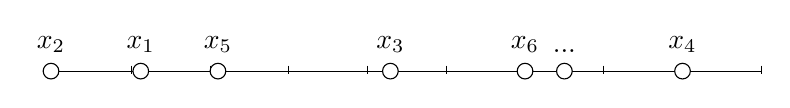
\begin{tikzpicture}
% a straight line segment
\draw (1,0) -- (10,0);
\foreach \x  in {1,...,10}
  \draw[xshift=\x cm] (0pt,2pt) -- (0pt,-1pt);
% the labels
\node[fill=white,draw=black,circle,inner sep=2pt,label=above:{$x_1$}] at (2.12,0) {};
\node[fill=white,draw=black,circle,inner sep=2pt,label=above:{$x_2$}] at (0.98,0) {};
\node[fill=white,draw=black,circle,inner sep=2pt,label=above:{$x_3$}] at (5.29,0) {};
\node[fill=white,draw=black,circle,inner sep=2pt,label=above:{$x_4$}] at (9,0) {};
\node[fill=white,draw=black,circle,inner sep=2pt,label=above:{$x_5$}] at (3.1,0) {};
\node[fill=white,draw=black,circle,inner sep=2pt,label=above:{$x_6$}] at (7,0) {};
\node[fill=white,draw=black,circle,inner sep=2pt,label=above:{...}] at (7.5,0) {};
\end{tikzpicture}
\end{center}

Escogemos el primer elemento $g_1$ de nuestra subsubcesión, y dividimos por la mitad el segmento.

\begin{center}
\begin{tikzpicture}
\draw (1,0) -- (10,0);
\foreach \x  in {1,...,10}
  \draw[xshift=\x cm] (0pt,2pt) -- (0pt,-1pt);
% the labels
\node[fill=black,draw=black,circle,inner sep=2pt,label=above:{$x_1$},label=below:{$g_1$}] at (2.12,0) {};
\node[fill=white,draw=black,circle,inner sep=2pt,label=above:{$x_2$}] at (0.98,0) {};
\node[fill=white,draw=black,circle,inner sep=2pt,label=above:{$x_3$}] at (5.29,0) {};
\node[fill=white,draw=black,circle,inner sep=2pt,label=above:{$x_4$}] at (9,0) {};
\node[fill=white,draw=black,circle,inner sep=2pt,label=above:{$x_5$}] at (3.1,0) {};
\node[fill=white,draw=black,circle,inner sep=2pt,label=above:{$x_6$}] at (7,0) {};
\node[fill=white,draw=black,circle,inner sep=2pt,label=above:{...}] at (7.5,0) {};

\draw[draw=red,ultra thick] (5.5,-1) -- (5.5,1);
\node[text=red] at (5.5,-1.3) {1};
\end{tikzpicture}
\end{center}

En al menos una de las dos mitades del segmento habrá infinitos términos: cogemos esa mitad y repetimos los mismos pasos. Finalmente, llegaremos a una subsucesión de este estilo:

\begin{center}
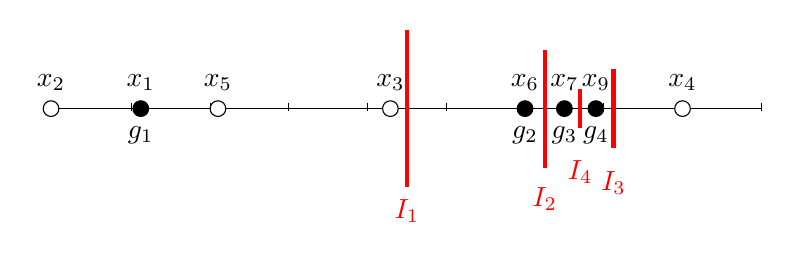
\begin{tikzpicture}
\draw (1,0) -- (10,0);
\foreach \x  in {1,...,10}
  \draw[xshift=\x cm] (0pt,2pt) -- (0pt,-1pt);
% the labels
\node[fill=black,draw=black,circle,inner sep=2pt,label=above:{$x_1$},label=below:{$g_1$}] at (2.12,0) {};
\node[fill=white,draw=black,circle,inner sep=2pt,label=above:{$x_2$}] at (0.98,0) {};
\node[fill=white,draw=black,circle,inner sep=2pt,label=above:{$x_3$}] at (5.29,0) {};
\node[fill=white,draw=black,circle,inner sep=2pt,label=above:{$x_4$}] at (9,0) {};
\node[fill=white,draw=black,circle,inner sep=2pt,label=above:{$x_5$}] at (3.1,0) {};
\node[fill=black,draw=black,circle,inner sep=2pt,label=above:{$x_6$},label=below:{$g_2$}] at (7,0) {};
\node[fill=black,draw=black,circle,inner sep=2pt,label=above:{$x_7$},label=below:{$g_3$}] at (7.5,0) {};
\node[fill=black,draw=black,circle,inner sep=2pt,label=above:{$x_9$},label=below:{$g_4$}] at (7.9,0) {};
\draw[draw=red,ultra thick] (5.5,-1) -- (5.5,1);
\node[text=red] at (5.5,-1.3) {$I_1$};

\draw[draw=red,ultra thick] (7.25,-0.75) -- (7.25,0.75);
\node[text=red] at (7.25,-1.15) {$I_2$};

\draw[draw=red,ultra thick] (8.125,-0.5) -- (8.125,0.5);
\node[text=red] at (8.125,-0.95) {$I_3$};

\draw[draw=red,ultra thick] (7.7,-0.25) -- (7.7,0.25);
\node[text=red] at (7.7,-0.8) {$I_4$};
\end{tikzpicture}
\end{center}

Nuestra subsucesión $\{g_x\}$ es igualmente infinita. Tal y como la hemos definido, tenemos que cada $g_i$ está en un intervalo $(I_i, I_{i-1})$ que cada vez se hace más pequeño. Es decir, que la subsucesión $\{g_x\}$ es de Cauchy y, por lo tanto convergente.

Ahora sólo queda ver cómo podríamos obtener esa subsucesión cuando estamos en espacios que no sean $\real^N$. La idea es sencilla: primero, buscamos una subsucesión que converja en la primera coordenada. Dentro de esa subsucesión, buscamos otra subsucesión que converja además en la segunda, y así con las $N$ coordenadas. 
\end{proof}

\begin{theorem} \label{thmCompactoMax} Sea $K\subset \real$ un conjunto compacto. Entonces, si $\appl{f}{\real}{\real}$ es continua en $K$ existen  $x_m,x_M \in K \tq F(x_m) \leq F(x) \leq F(x_M)\;\forall x \in K$.

Es decir, si $F$ es continua en $K$ alcanza su máximo y su mínimo en el conjunto.
\end{theorem}

\paragraph{Aplicación:}
$F(\gor{x}) = |||\gor{x}|||$ una norma (que ya sabemos que es continua):

\emph{Conclusión:} $m \md{x} \leq |||\gor{x}||| \leq C||\gor{x}||$

\begin{theorem}
En $\real^N$ TODAS las normas son equivalentes. 
\end{theorem}

\subsubsection{Conexión}
\begin{defn}[Conexión\IS por caminos]
Dados $a,b \in C$ podemos encontrar una aplicación continua $\appl{\varphi}{[0,1]}{\real^N}$ tal que $\varphi(0) = a$ y  $\varphi(1) = b$ con $ \varphi(t) \in C\, \forall t \in [0,1]$. 

Es decir, $C$ es conexo por caminos si podemos encontrar una "línea", un camino que una dos puntos cualquiera del conjunto y que además no se salga del conjunto.
\end{defn}

\begin{defn}[Conexión\IS por abiertos]
$C$ es conexo por conjuntos si para cualquier par de abiertos $A,B \subset \real^N \tq C\subset A\cup B$ se cumple que, si $A\cap C\neq \emptyset \y B\cap C \neq \emptyset $ entonces $ A\cap B \neq \emptyset$.

Esto es equivalente a decir que $C$ no puede ser expresado como unión de dos conjuntos disjuntos.
\end{defn}


\begin{remark}

\begin{figure}[hbtp]
\label{imgPeine}
\begin{center}
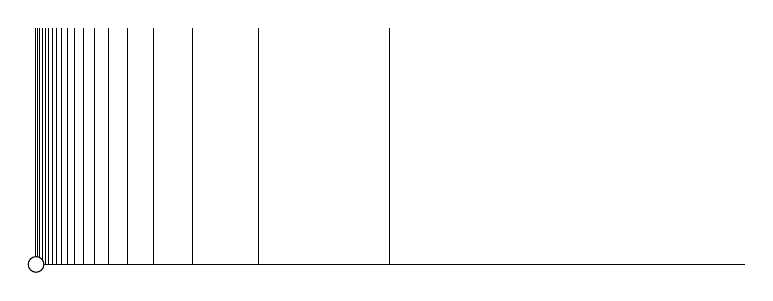
\begin{tikzpicture}

\draw (1,0) -- (10,0);

\foreach \x  in {2,...,20}
  \draw ($10/\x*(1,0) + (0.49,0)$) -- ($(0.49,3) + 10/\x*(1,0)$);

\node[fill=white,draw=black,circle,inner sep=2pt] at (1,0) {};

\end{tikzpicture}
\caption{Conjunto peine}
\end{center}
\end{figure}

Es curioso comprobar que estas 2 definiciones no son equivalentes. Tomemos el conjunto peine (figura \ref{imgPeine})
\[ \left\{(x,0), x\in (0,1]\right\} \cup \{(0,y), y \in (0,1]\} \cup \left\{\bigcup_{n=1}^{\infty}{\left(\frac{1}{n},y\right), y \in [0,1]}\right\} \]

Es un conjunto conexo por abiertos porque no podemos separarlo en dos conjuntos disjuntos. Sin embargo, no es conexo por caminos porque, si queremos ir del punto $(0,1)$ al $(0,0.5)$ no podemos hacerlo ya que el único camino pasaría por el punto $(0,0)$, que no está en el conjunto.
\end{remark}

\subsection{Funciones continuas, abiertos y cerrados}
 
 Al tener definida una norma de vectores podemos definir convergencia y continuidad:

\begin{defn}[Convergencia] Se dice que $\gx_n$ converge a $\gx$ (notación: $\gx_n \to \gx$) si

\[  \forall \varepsilon > 0\; \exists n_0 \tq n > n_0 \implies \md{\gx-\gor{x}_n}<\varepsilon \]

\end{defn}

\begin{defn}[Función\IS continua] Sea $\appl{F}{\real^N}{\real^M}$. Se dice que $F$ es continua en $a$ si y sólo si 

\[  \forall \varepsilon > 0 , \exists \delta > 0 \tq \md{\gx-\ga}_a < \delta \Rightarrow \md{F(\gx)-F(\ga)}_b< \varepsilon \]
\label{dfnContinua}
\end{defn}

\begin{remark} Es interesante ver que se puede hablar de continuidad tomando una norma en $\mathbb{R}^N$ y otra distinta en $\real^M$ sin por ello variar la definición de continuidad, teniendo en cuenta que todas las normas son equivalentes. \end{remark}

A partir de esta definición podemos estudiar qué hacen las funciones continuas con conjuntos abiertos y cerrados. Sea $F$ continua. Contrario a lo que podríamos intuir, 

\begin{enumerate}
\item A abierto no implica que  $F(A)$ sea abierto.
\item B cerrado no implica que $F(B)$ sea cerrado.
\end{enumerate}

Empezamos definiendo en qué consiste una función inversa:

\begin{defn}[Función\IS inversa] Dada \[\appl{F}{\real^N}{\real^N}\], definimos su inversa como
\[ \inv{F}(A) = \left\{\gor{x}\in \real^N \tq F(\gor{x})\in A\right\} \]
\end{defn}

A partir de aquí podemos extraer dos conclusiones que sí nos ayudarán a discernir si un conjunto imagen es abierto y cerrado.

\begin{theorem}[Función\IS inversa]\par\noindent\par
\label{thmInversa}
\begin{itemize}
\item F continua y A abierto $\implies F^{-1} (A)$ abierto.
\item F continua y B cerrado $\implies F^{-1} (A)$ cerrado.
\end{itemize}
\end{theorem}

Este teorema nos sirve para decir fácilmente si un conjunto es abierto o cerrado. Por ejemplo, consideremos
 \[ M=\{(x,y,z) \in \real^3 \tq x^2 + \cos\left(x\abs{y}\right) - e^z < 1 \} \]

Podemos definir ahí la función $F$ como 
\[ F(x,y,z) = x^2 + \cos\left(x\abs{y}\right) - e^z\]

que va de $\real^3$ a cierto conjunto $A = \{ a \in \real \tq a < 1 \}$. Podemos reescribir $M$ como
\[M=\{(x,y,z) \in \real^3 \tq  F(x,y,z) \in A\}\]

o, de otra forma, $M = \inv{F}(A)$. Según el teorema (\ref{thmInversa}), como $A$ es abierto entonces $M$ también es abierto.

\begin{proof} Demostramos las dos implicaciones que hemos enunciado.

1) Dado un $\gor{x} \in F^{-1} (A)$ queremos hallar un $R>0$ tal que $B_R(\gor{x})\subset F^{-1} (A)$. Partimos de 
\[\gor{x}\in F^{-1} (A) \dimplies F(\gor{x})\in A\]

Como $F$ es continua, $\exists \varepsilon>0 \tq B_{\varepsilon}(F(\gor{x}))\subset A$. Esto es equivalente a decir que, para cualquier $\gz$
\[ ||\gor{z}-F(\gor{x})|| < \varepsilon \implies \gor{z}\in A\]

Por la definición de continuidad (\ref{dfnContinua}), dado un $\gor{s}\in B_R(\gor{x})$ 

\[ \exists \delta > 0 \tq ||\gor{x}-\gor{s}||<\delta \implies ||F(\gor{x})-F(\gor{s})||< \varepsilon \]


y por lo tanto $F(\gor{s}) \in A$ y $\gor{s} \in F^{-1} (A)$.
Conclusión: Hemos encontrado un $\delta > 0$ tal que $s \in B_R(\gor{x}) \implies s \in F^{-1} (A)$.
\end{proof}

\section{Aplicaciones lineales y matrices}

\subsection{Aplicaciones lineales}

\begin{defn}[Aplicación\IS lineal]

Sea: $\appl{L}{\real^N}{\real^M}$. Entonces, $L$ es lineal si y sólo si

\[ L(\lambda \gor{x}) = \lambda L(\gor{x}) \] 
\[ L(\gor{x}+\gor{y}) = L(\gx)+L(\gy)\] 

\end{defn}
Además, toda aplicación lineal se puede escribir en forma de matriz.

\[L(\gor{x})=A\gor{x} =
\begin{pmatrix}
a_{11} 	& \cdots & a_{1n}		\\
\vdots	& \ddots &  \vdots 	\\
a_{n1}	& \cdots & a_{nn} 
\end{pmatrix}\]

\begin{theorem}
Toda aplicación lineal $L$ es continua.
\end{theorem}
\begin{proof} Partiendo de la definición de continuidad (\ref{dfnContinua}), $L$ es continua si y sólo si

\[ \forall \ga, \gx \; \forall \epsilon > 0 \; \exists \delta > 0 \tq \md{\ga - \gx} < \delta \implies \md{L\ga - L\gx} < \epsilon \]

Sabemos que $\md{A\gx} ≤ C\md{\gx}$ para alguna constante $C$. Podemos reescribir

\[ \md{L\ga - L\gx} = \md{L(\ga-\gx)} ≤ C\md{\ga-\gx} \]

Entonces, la igualdad se cumple si tomamos $\epsilon = C\delta$.
\end{proof}

\subsection{Norma de matrices}
Consideramos una aplicación continua

\begin{align*}
\appl{F}{\real^N&}{\real} \\
\gor{x} &\longrightarrow F(\gx) = \underbrace{||A\gx||}_{L(\gx)}
\end{align*}

Sabemos que existe $C>0$ tal que $||A\gx|| \leq C||\gx||$, es decir,  $||A\gx||\leq C$ si $||\gx||=1$. Queremos saber cuál es la mejor constante que podemos encontrar, la que más se ajuste. Consideramos el conjunto $M$ de todos los vectores de la esfera unidad, es decir 

\[ M = \{||A\gx|| \tq ||\gx||=1\}\subset \real \]

Entonces mejor constante $C$ es la cota superior mínima (supremo) que vamos a llamar $\alpha$. Al ser $F$ continua y $M$ compacto, sabemos que el supremo $\alpha \in M$.

\begin{defn}[Norma\IS de una matriz]
$$\norm{A} = \alpha = \max{\norm{A\gx} \tq \norm{\gx} =1}$$
\end{defn}

\begin{proof} Hay que demostrar que esta norma que hemos definido cumple las propiedades de una norma (\ref{defnNorma}). Las dos primeras son triviales, demostremos la desigualdad triangular
\[ \norm{A+B} = \max{\norm{(A+B)\gx}} = \norm{(A+B)\gx_{A,B}} \] 

donde $\gx_{A,B}$ es el vector que da el valor máximo para esa multiplicación. Usando la propiedad asociativa

\[  \norm{(A+B)\gx_{A,B}} = \norm{A\gx_{AB} + B\gx_{A,B}} ≤ \norm{A\gx_{A,B}} + \norm{B\gx_{A,B}} \]

Sabemos que existen dos vectores $\gx_A$ y $\gx_B$ que maximizan el resultado $\norm{A\gx_A}$ y $\norm{A\gx_B}$ respectivamente, por lo tanto

\[ \norm{A\gx_{A,B}} + \norm{B\gx_{A,B}} ≤ \norm{A\gx_A} + \norm{B\gx_B} = \norm{A} + \norm{B} \]

\end{proof}

Basándonos en lo que hemos obtenido, calculamos la norma uno de 
\[A = \begin{pmatrix}
      1&2\\-3&1\\2&0
     \end{pmatrix}\]  

Tenemos que maximizar, sabiendo que $|x|+|y| = 1$:

\[ |x+2y| + |-3x+y| + |2x| \leq |x|+|2y| + |3x| + |y| + 2|x| = 6|x|+3|y| \leq 6 (|x|+|y|) =6 \]
¿Podemos encontrar un vector $\gx = (x_0,y_0)$ tal que $||A(x_0,y_0)^T||_1 = 6$?\\
Tomando $x_0 = 1$ y $y_0 = 0$ lo encontramos. Como $\gx$ está en la esfera unidad y es una cota, es el máximo y por lo tanto la norma que buscamos.

Curiosamente, \textbf{coincide con la suma de los valores absolutos de las columnas} y escoger el más grande.

Si tomamos la norma infinito de 
\[A = \begin{pmatrix}
      1&2\\-3&1\\2&0
     \end{pmatrix}\]

Tenemos que \textbf{coincide con el máximo de las posibles sumas de los valores absolutos de las filas}.



Queremos buscar ahora cuánto vale la norma de una matriz cuando usamos la norma euclídea. Usaremos los dos lemas siguientes para apoyarnos.

\begin{lemma}
 Sea A una matriz cualquiera, entonces $\trans{A}A$ es simétrica.
\end{lemma}
\begin{lemma}
 \[ \underbrace{\pesc{\gx,A\gy}}_{\text{Producto en } \real^n} = \underbrace{\pesc{A^T \gx,\gy}}_{\text{Producto en } \real^M} \]
\end{lemma}

Tenemos $A^TA$ diagonalizable, de dimensión $N \times N$. Buscamos cuánto vale $\norm{A\gx}$ con  $\gx \in \real^N$. Empezamos desarrollando el vector en una base ortonormal de  $A^T A$: \[ \gx = \sum \alpha_i \gv_i \] y por lo tanto \[ ||\gx|| = \sum \alpha_i^2 \pesc{\gv_i,\gv_i}\].
 
 Desarrollamos el producto \[\trans{A}A\gx = \trans{A}A\left(\sum \alpha_i \gv_i\right) = \sum \left(\alpha_i\lambda_i\gor{v}_i\right) \] donde $\lambda_i$ son los autovalores de $\trans{A}A$. 
 
 Ahora queremos hallar el máximo de $||A\gx||$ cuando $||\gx|| = 1$:
 
 \[ ||A\gx||^2 = \pesc{A\gx,A\gx} = \pesc{\trans{A}A\gx,\gx} = \pesc{\sum \lambda_i \alpha_i \gv_i,\sum\alpha_i \gv_i} \]
 
 Como la base de $\{\gv_n\}$ es ortonormal, $\pesc{\gv_i, \gv_j} = 0$ si $i≠j$, por lo tanto sólo nos queda
 \[ \pesc{\sum \lambda_i \alpha_i \gv_i,\sum\alpha_i \gv_i} = \sum \lambda_i \alpha_i^2 \leq \lambda_{max} \left(\sum \alpha_i^2\right) = \lambda_{max} \]
 
 teniendo en cuenta que $\norm{\gx} = 1$ y donde $\lambda_max$ es el autovalor máximo. Es decir, hemos llegado a que
 \[ \max\norm{A\gx} ≤ \sqrt{\lambda_{max}} \]
 
 Hemos definido una cota para $\norm{A\gx}$. Ahora bien, esa cota se alcanza cuando $\gx$ es el autovector asociado a $\lambda_{max}$, por lo tanto la cota es un máximo y la norma de la matriz.
 
 \section{Límites}
 
 \begin{defn}[Límite] Dada una función $\appl{F}{\real^N}{\real^M}$, definimos su límite cuando $\gx\to\ga$ de la siguiente forma:
  \[ \lim_{\gx \rightarrow \ga} F(\gx) = \gor{L} \dimplies \forall \varepsilon > 0,  \exists \delta>0 \tlq 0<||\gx-\ga|| <\delta \implies ||F(\gx) - L||<\varepsilon\] 
 \end{defn}
 
 Importante el detalle de $0 < ||\gx-\ga||$, no es un $\leq$, porque no se necesita que la función esté siquiera definida en el punto $\ga$.  
 
 \begin{theorem}[Convergencia\IS de coordenadas]
  
  Sean $\gor{x}_n = (x_1,...,x_n) \in \real^N$ y $\gor{L} = (L_1,...,L_n) \in \real^N$. Entonces
 
  \[ x_n \rightarrow \gor{L} \dimplies (x_1 \rightarrow L_1) \y (x_2 \rightarrow L_2) \y ... \y (x_n \rightarrow L_n) \]
 \end{theorem}
 
 Idea para el cálculo de límites: 
 \begin{itemize}
  \item $\displaystyle\mylim{x}{a}{x} = \lim_{\gy\rightarrow 0} F(\gy+\ga)$.
  \item Límite a lo largo de rectas. $\displaystyle\mylim{x}{a}{\gx} \sim \lim F({t\gor{v}})$
 
 \end{itemize}
 
 Si $\displaystyle\lim F({t\gor{v}})$ toma valores distintos dependiendo de $\gor{v}$ entonces $\nexists \displaystyle\mylim{x}{0}{\gx}$
 
Por otra parte, si $\forall t \in \real, \mylim{x}{a}{t\gor{v}} = L$, entonces $\gor{L}$ es el candidato a ser el límite (no tiene por qué serlo). El siguiente paso sería demostrar con argumentos de comparación (Sandwich) u otros que $\mylim{x}{a}{\gx} = L$.
 
 El contraejemplo para ver que la existencia del límite por rectas no implica la existencia del límite es estudiar la función \[ f(x,y) = \frac{x y^2}{x^2 + y^4}\] . Veamos por qué.
 
 Si os acercamos al límite por medio de rectas:

 \[ f(x,y) = f(x,mx) = \frac{x\cdot(mx)^2}{x^2 + (mx)^4} = \frac{m^2x^3}{(1 + x^2m^4)x^2} \]
 \[ \lim{x\to 0} (f(x,mx)) \rightarrow 0, \forall m \in \real \]

 Pero si nos acercamos al límite por medio de $x = y^2$ tenemos:

\[ f(x,y) = f(y^2,y) = \frac{y^2y^2}{y^4+y^4} = \frac{y^4}{2y^4} = \frac{1}{2} ≠ 0\]  

Por lo tanto, el límite no existe a pesar de que existe cuando nos acercamos por rectas.
 
 
\begin{theorem}
 $F$ es continua si y sólo si para cualquier abierto $A$, $F^{-1}(A)$ es abierto.
\end{theorem}

\begin{proof}
De este teorema ya teníamos demostrada la implicación a la derecha (\ref{thmInversa}), así que sólo falta demostrar hacia la izquierda. Queremos probar que

\[ \forall \varepsilon > 0\; \exists \delta>0 \tlq ||\gx-\ga||<\delta \implies ||F(\gx)-F(\ga)||<\epsilon \]

Tomamos  \[ A = B_{\varepsilon}(F(\ga))\] de tal forma que \[ F(\ga) \in A \implies \ga \in F^{-1}(A) \]

Por hipótesis, $F^{-1}(A)$ abierto y $\ga \in F^{-1}(A)$ . Entonces 
\[\exists B_{\delta}(\ga) \subset F^{-1}(A) \].Es decir, \[ \gor{s}\in B_{\delta}(\ga) \subset F^{-1}(A), s\in F^{-1}(A) \implies F(s) \in A = B_{\varepsilon}(F(\ga))\]
\end{proof}

\begin{remark}
Este teorema también se cumple para cerrados.
\end{remark}

\section{Diferenciación}

\begin{defn}[Función\IS diferenciable]
 $F$ es diferenciable en $\gor{a}$ si existe una aplicación lineal $L$ tal que

\[ \frac{F(\gx)-F(\ga)-L(\gx-\ga)}{||\gx-\ga||} \convs[][\gx][\ga] 0 \]

que se puede expresar como
\[ \lim_{\gor{h} \rightarrow \gor{0}} \frac{\md{F(\ga+\gor{h}) - F(\ga) - L\gor{h}}}{||\gor{h}||} = 0 \]
\end{defn}

\begin{defn}[Diferencial]
A esa matrix $L$ la vamos a llamar la diferencial de $F$ en $\ga$:

\[ L\equiv DF(\ga) \]
\end{defn}

\begin{theorem}
$$F \text{ diferenciable en } \ga \implies F \text{ continua en } \ga$$
\end{theorem}

\begin{proof}
 $$\lim_{\gor{h} \rightarrow \gor{0}} \frac{\md{F(\ga+\gor{h}) - F(\ga) - L\gor{h}}}{\md{\gor{h}}} = 0$$
 Esta es la definición de diferenciable. Para que este límite sea 0, el numerador tiene que tender a 0, por lo que $F(\ga+\gor{h}) - F(\ga) \rightarrow 0$
\end{proof}


\begin{theorem}
Si la diferencial existe, entonces es única.
\end{theorem}

\begin{proof}  Vamos a demostrar que esa aplicación $L$ es única. Supongamos que existen $L_1,L_2$ que cumplen las condiciones.
\[0=\lim_{\gor{h} \rightarrow \gor{0}} \frac{F(\gor{a}+\gor{h}) - F(\ga)-L_1\gor{h}}{||\gor{h}||} = \lim_{\gor{h} \rightarrow \gor{0}} \frac{F(\gor{a}+\gor{h}) - F(\ga)-L_2\gor{h}}{||\gor{h}||}\].

Sumando:

\[ 0 = \lim_{\gor{h} \rightarrow \gor{0}} \frac{||F(\gor{a}+\gor{h}) - F(\ga)-L_1\gor{h}|| + ||F(\gor{a}+\gor{h}) - F(\ga) -L_2\gor{h}||}{||\gor{h}||} \]

Teniendo en cuenta que $||A-B|| = ||A+(-B)|| \leq ||A||+||B||$

\[ 0 \leq \lim_{\gor{h} \rightarrow \gor{0}} \frac{2\cdot\md{F(\ga + \gor{h}) - F(\ga)} + \md{L_1\gor{h}} + \md{L_2\gor{h}}}{\md{\gor{h}}} \]

\textit{Aquí falta completar.}
\end{proof}



\paragraph{Nomenclatura: }
Aproximación lineal $\sim$ Diferencial.

Matriz jacobiana $\sim$ Jacobiana.

\begin{defn}[Matriz\IS diferencial]
 Matriz asociada a $DF(\ga) \equiv $ Matriz de las derivadas parciales de F.

 $$DF(\ga) \equiv \begin{pmatrix}
                \dpa{F_1}{x_1} & \cdot & \dpa{F_1}{x_N}\\
                \vdots& \ddots & \vdots\\
                \dpa{F_N}{x_1} & \cdot & \dpa{F_N}{x_N}
                \end{pmatrix}
$$
\end{defn}

\begin{theorem}
 $F$ diferenciable en $\ga \implies \exists \deriv{F_k}{x_i}(\ga), i=1,2,...,N \y k = 1,2,...,M$
\end{theorem}

El contraejemplo para demostrar la implicación a la izquierda es el mismo que en los límites a lo largo de rectas.

$f(x,y) = \left\{ \begin{matrix}
\displaystyle\frac{xy^2}{x+y^2} & (x,y) \neq (0,0) \\
0 & (x,y)=(0,0)

          \end{matrix}\right.
$

Según las aplicaciones que tengamos, la diferencial se suele llamar de una u otra forma. Con $\appl{\delta}{\real}{\real^M}$ utilizamos notación vectorial en vez de matricial porque tendríamos una matriz columna. Por ejemplo: la velocidad (en un instante de tiempo, un punto en el espacio).

\begin{defn}[Gradiente] Sea $\appl{F}{\real^N}{\real}$, entonces definimos el vector gradiente como

\[ \grad F(\gx) = DF(\gx) = \left(\dpa{F}{x_1}, \dpa{F}{x_2},\dotsc, \dpa{F}{x_n}\right) \]
\end{defn}


\subsection{Regla de la cadena}
\index{Regla!de la cadena}
Consideremos la composición de dos funciones de la siguiente forma:

$\appl{F}{\real^N}{\real^M}$.

$\appl{G}{\real^M}{\real^K}$.

$\appl{H=G\circ F}{\real^N}{\real^K}$.

$ \gx \in \real^N, \gy \in \real^M$

\begin{wrapfigure}{r}{0.3\textwidth}
\begin{center}
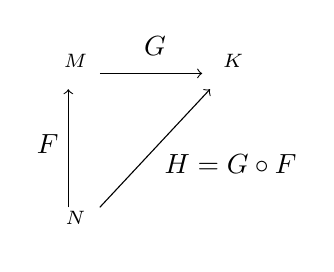
\begin{tikzpicture}
\draw[->] (-0.1,0.2) -- (-0.1,1.7);
\draw[->] (0.3,1.9) -- (1.6,1.9);
\draw[->] (0.3,0.2) -- (1.7,1.7);

\node at (0,0) {$\real^N$};
\node at (0,2) {$\real^M$};
\node at (2,2) {$\real^K$};

\node[left] at (-0.1,1) {$F$};
\node[above] at (1,2) {$G$};
\node[below right] at (1,1) {$H = G\circ F$};
\end{tikzpicture}
\end{center}
\caption{Composición de funciones}
\end{wrapfigure}

Con $F$ diferenciable en $\ga$ y $G$ diferenciable en $F(\gor{a})$. Entonces $H=G\circ F$ es diferenciable en $\ga $.
Además la expresión matricial es:

\[ \underbrace{DH(\ga)}_{K\times N} = \underbrace{DG(F(\ga))}_{K\times M}\cdot \underbrace{DF(\ga)}_{M\times N} \]

No hace falta calcular toda la matriz si sólo queremos un elemento. Para calcular 1 único elemento de la matriz diferencial (el de la fila $i$, columna $j$), usamos la siguiente fórmula
\[ \dpa{H_i}{x_j}(\ga) = \sum_{k=1}^M \dpa{G_i}{y_k}\cdot\dpa{F_k}{x_j} \]

Siempre teniendo en cuenta que $\displaystyle\dpa{G_i}{y_k}$ está evaluado en $F(\ga)$ y $\displaystyle\dpa{F_k}{x_j}$ está evaluado en $\ga$.

\subsection{Extensiones del Teorema del Valor Medio}

El teorema anterior que vimos del valor medio era para funciones de una variable, y proponía lo siguiente:
\begin{theorem}[Teorema\IS del valor medio (una variable)]
\label{thmTVM1var}
Dada $\appl{f}{\real}{\real}$ diferenciable, se tiene que \[ f(b)-f(a) = f'(c)(b-a)\] para algún $c\in[a,b]$
\end{theorem}

Después el teorema lo extendimos a funciones de $\real^N$ en $\real$: dada $\appl{F}{\real^N}{\real}$ entonces definíamos

 \[ \sigma(t)  = t\gor{b}+(1-t)\gor{a} \]

 y $g = F\circ \sigma$ era una aplicación de los reales a los reales, y entonces aplicando el teorema anterior teníamos que

 \[ F(\gor{b}-\gor{a}) = g(1)-g(0)  = g'(s) \]
 para algún $s\in[0,1]$.

Sin embargo, al tratar de extrapolar este resultado a una función $\appl{F}{\real^N}{\real^2}$ nos queda que

 \[ F(\gor{b})-F(\ga) = \begin{pmatrix}
                         \pesc{\nabla F_1(\gor{c_1}),{\gor{b}-\ga}}\\
                         \pesc{\nabla F_2(\gor{c_2}),\gor{b}-\ga}
                        \end{pmatrix}
 \]
  Tenemos 2 $c$ distintos, uno para cada $f$, por lo que este teorema pierde sentido. Hay que buscar una extensión, otra formulación del teorema que nos permita aplicarlo a las funciones que estamos estudiando.

  \begin{theorem} [Teorema\IS del valor medio (varias variables)]
  \label{thmTVM}
  Sea $f \in C^1$ en un abierto que contenga $[a,b]$. Entonces

  \[ \norm{F(\gor{b})-F(\ga)} \leq \md{DF(\gor{c})} \cdot \md{\gor{b}-\ga} \]

  Siendo $c$ un punto del segmento que une $\ga$ y $\gb$ en el que $\md{DF(tb+(1-t)a)}$ alcanza su máximo.
  \end{theorem}

  \begin{proof}

Primero vamos a demostrar la siguiente desigualdad:

\begin{equation}
\label{eqnTVM1}
 \md{\int_0^1 F(t) \,dt}≤ \int_0^1 \md{F(t)}\,dt
\end{equation}

Si tomamos \[ L = \int_0^1 F(t) \,dt \]  entonces

\[ \md{L}^2 = \md{\int_0^1 F(t) \,dt}^2 = \pesc{L,\int_0^1 F(t) \,dt} \]

Como $L$ es un vector constante, podemos meterlo en la integral y tenemos que

\[ \pesc{L,\int_0^1 F(t) \,dt} = \int_0^1 \pesc{L, F(t)} ≤ \int_0^1 \md{L}\md{F(t)} = \md{L} \int_0^1 \md{F(t)} \]

y por lo tanto

\begin{gather*}
\md{L}^2 ≤ \md{L} \int_0^1 \md{F(t)} \\
\md{L} ≤ \int_0^1 \md{F(t)} \\
\md{\int_0^1 F(t) \,dt } ≤ \int_0^1 \md{F(t)}
\end{gather*}

quedando así demostrada la desigualdad (\ref{eqnTVM1}).

Consideramos ahora

\[ \md{F(\gb) - F(\ga)} \]

Si integramos $DF$ por el camino que va de $\ga$ a $\gb$ nos queda que

\[ \md{F(\gb) - F(\ga)} = \md{\int_0^1 DF\left[\ga(1-t) + t\gb\right](\gb - \ga)\, dt } \]

que por (\ref{eqnTVM1})

\[ \md{F(\gb)-F(\ga)} ≤ \int_0^1 \md{DF\left[\ga(1-t) + t\gb\right](\gb - \ga)}\, dt  \leq  \int_0^1 \md{DF\left[\ga(1-t) + t\gb\right]}\md{\gb - \ga}\, dt \]

Nos fijamos en $\md{DF\left[\ga(1-t) + t\gb\right]}$. Al ser continua y estar definida en un conjunto compacto, entonces alcanza su máximo en algún punto $\gor{c}$ entre $\ga$ y $\gb$, por lo tanto

\[ \md{F(\gb) - F(\ga)} ≤  \int_0^1 \md{DF(\gor{c})}\md{(\gb - \ga)} = \md{DF(\gor{c})}\md{\gb - \ga} \]
  \end{proof}

Este teorema nos sirve, por ejemplo, para ver que si tenemos $\appl{F}{\real^N}{\real^M}, F \in C^1$, definida en un conjunto abierto y conexo y  $DF(\gx) \equiv 0\; \forall\gx$, entonces $F$ es constante.

\subsection{Derivada direccional}

$\appl{F}{\real^N}{\real^M}$ (escalar)

$\ga \sim$ Recta que pasa por $\ga$ con dirección $\gor{v}$.

$r(t) = \ga + t\gor{v}$.

\obs
Como una recta tiene infinitos vectores directores (dependiendo de la longitud), siempre tomaremos vectores directores unitarios, con $\norm{\gor{v}} = 1$.


Vamos a estudiar: $g(t) = F(\ga + t\gor{v}) = F \circ r (t)$.

$t \sim 0 \dimplies \ga + t\gor{v} \sim \ga$
\begin{defn} [Regla de la cadena]
$$g'(0) = \displaystyle\lim_{h \rightarrow 0} \frac{g(h)-g(0)}{h} = \displaystyle\lim_{h \rightarrow 0} \frac{F(\ga+h\gor{v})-F(\ga)}{h} \equiv D_{\gor{v}}F(\ga)$$.
\end{defn}

\obs
La existencia de $D_{\gor{v}}F(\ga), \forall \gor{v}\in \real^N$ NO garantiza que $F$ sea derivable.


Si sabemos que $F$ SÍ es diferenciable podemos usar la regla de la cadena obteniendo:

$D_{\gor{v}}F(\ga) = g'(0) = D(F\circ r)(0) = ... = \pesc{\nabla F(\ga),\gor{v}}$


\paragraph{Aplicación:}
\begin{itemize}
 \item
 Dirección de máximo crecimiento:

$D_{\gor{v}}F(\ga) = \pesc{\nabla F(\ga),\gor{v}}\leq \norm{\nabla F(\ga)}\cdot \underbrace{\norm{\gor{v}}}_{\equiv 1}$

Conclusión:
\begin{align*}
D_{\gor{v}}F(\ga) &\leq \norm{\nabla F(\ga)}\\
&\uparrow\\
\text{El }= \text{se obtien}&\text{e cuando }\gor{v} = \displaystyle \frac{\nabla F(\ga)}{\norm{\nabla F(\ga)}}.
\end{align*}


 \item
 Vector perpendicular a los conjuntos de nivel

 $\appl{F}{\real^N}{\real^M}$

 $S = \{ \gx \in \real^N \tq F(\gx) = 0\}$ (Conjunto de nivel)

 $\ga \in S$

 Entonces: $\nabla F(\ga) \perp S$
\end{itemize}

\begin{theorem}[Derivadas parciales continuas implican función diferenciable]
Si existen todas las derivadas parciales y son continuas $\implies F$ diferenciable en $\ga$.

\end{theorem}

Contraejemplo de la no reciprocidad: $f(x) = x^2 sin\left(\frac{1}{x}\right)$

\begin{proof}
 $\appl{F}{\real^2}{\real}$

 $$¿\frac{\left|F(a+a,b+k) - F(a,b) - \deriv{F}{x}(a,b) h - \deriv{F}{y}(a,b)k\right|}{\norm{(h,k)}}\longrightarrow 0?$$

 Sumamos y restamos al numerador $F(a,b+k)$.

 $$\frac{\left|\left(\underbrace{F(a+h,b+k) - F(a,b+k)}_{\deriv{F}{x}(a+\tilde{h},b+k) \text{ para algún } 0 \leq\tilde{h}\leq h} -  \deriv{F}{x}(a,b) h\right) + \left(\underbrace{F(a,b+k) - F(a,b)}_{\deriv{F}{x}(a+h,b+\tilde{k}) \text{ si } 0 \leq\tilde{k}\leq k}- \deriv{F}{y}(a,b) k\right)\right|}{\sqrt{h^2+k^2}}$$

 $$0\leq\frac{\left|\deriv{F}{x}(a+\tilde{h},b+k)-\deriv{F}{x}(a,b)\right| \cdot |h| + \left| \deriv{F}{y}(a,b+\tilde{k}) - \deriv{F}{y}(a,b)\right| \cdot |k|}{\sqrt{h^2+k^2}} = (*)$$

 Aquí es donde aplicamos que las derivadas parciales son continuas: como $h$ y $k$ son pequeños (por lo tanto $\tilde{h}<h$ también lo será) los puntos $(a,b)$ y $(a+h,b+k)$ también están cerca, por lo que sus imágenes por la derivada estarán también cerca, es decir, $|\deriv{F}{x}(a,b)-\deriv{F}{x}(a+\tilde{h},b+k)| \rightarrow 0$ y lo mismo con la otra.

 Conclusión:

 \begin{align*}
0 \leq (*) \leq \varepsilon \frac{|h|+|k|}{\sqrt{h^2+k^2}} &\leq C\varepsilon \rightarrow 0 \text{ cuando } \gor{h},\gor{k} \rightarrow \gor{0}\\
&\uparrow\\
\text{El numerdador es la} & \text{ norma 1 y el denominador la norma 2.}\\
\text{En } \real^N &\text{ todas las normas son equivalentes.}
 \end{align*}


\end{proof}


\subsection{Derivadas iteradas}

\paragraph{Notación:}

$\deriv{}{y}\left(\deriv{f}{x}\right) \equiv \deriv{^2f}{x \partial y}$

\begin{theorem}[Euler (orden de las derivadas)]
Si las derivadas segundas son continuas, entonces:
$$\deriv{^2f}{x_i\partial x_j} = \deriv{^2 f}{x_j \partial x_i}$$
\end{theorem}

\subsection{Máximos y mínimos}

\index{Máximo/mínimo!local}
\begin{defn}[Máximo/mínimo local] Sea $\appl{f}{\real^N}{\real}$. Diremos que $\vx_0 \in \real^N$ es un punto de máximo local si $\exists \epsilon > 0 \tq F(\vx_0) \geq F(\vx)\;\; \forall \vx \in B_{\epsilon} (\vx_0) $

La definición es análoga para el mínimo\end{defn}

\begin{remark} Por las propiedades del gradiente, si $F$ es diferenciable y $\vx_0$ es un máximo o mínimo local, entonces debe ser $\nabla F(\vx_0) = \vec{0}$.\end{remark}

\index{Punto!crítico}
\begin{defn}[Punto crítico] $\vx \in \real^N$ es un punto crítico de $F$ si y sólo si $\nabla F(\vy) = \vec{0}$\end{defn}

No todos los puntos críticos son máximos o mínimos, así que tenemos que clasificarlos de alguna forma. Para ello, usamos el polinomio de Taylor de orden 2, de forma que 

\[F(x,y) = F(x_0, y_0) + \pesc{\nabla F(x_0, y_0), (x-x_0, y-y_0)} +\]\[\frac{1}{2}(x-x_0, y-y_0)\left(\begin{matrix} \frac{\partial^2 f}{∂ x^2} (x_0,y_0) & \frac{\partial^2 f}{\partial x \partial y} (x_0,y_0) 
\\ \frac{\partial^2 f}{\partial y \partial x} (x_0,y_0) & \frac{\partial^2 f}{\partial y^2} (x_0,y_0) \end{matrix}\right) \left(\begin{matrix} x - x_0 \\ y - y_0 \end{matrix}\right) + \epsilon \]

Simplificando nos queda que:

\[F(\vx) = F(\vx_0) + \pesc{\nabla F(\vx_0),\vx - \vx_0} + \frac{1}{2}(\vx - \vx_0) D^2F(\vx_0) (\vx - \vx_o) ^T + \epsilon\]

Dado que el gradiente es 0, el punto clave es el signo de $\frac{1}{2}(\vx - \vx_0) D^2F(\vx_0) (\vx - \vx_o) ^T$. Para ello, usamos las siguientes definiciones del álgebra lineal.

\subsubsection{Resultados de álgebra lineal}
\index{Matriz!semidefinida positiva/negativa}
\index{Matriz!definida positiva/negativa}
\begin{defn}[Matriz semidefinida y definida positiva y negativa]\noindent\\ \indent
La matriz $A$ de dimensión $N\x N$ es semidefinida positiva si y sólo si $\vv A \vv^T \geq 0 \;\; \forall \vv \in \real^N$.

La matriz $A$ de dimensión $N\x N$ es definida positiva si y sólo si $\vv A \vv^T > 0 \;\; \forall \vv ≠0 \in \real^N$.

La matriz $A$ de dimensión $N\x N$ es semidefinida negativa si y sólo si $\vv A \vv^T \leq 0 \;\; \forall \vv \in \real^N$.

La matriz $A$ de dimensión $N\x N$ es definida negativa si y sólo si $\vv A \vv^T < 0 \;\; \forall \vv ≠0 \in \real^N$.
\end{defn}

\begin{theorem}
Si una matriz es simétrica, existe una base en la cual la matriz es diagonal.
\end{theorem}

\index{Autovalor}
\index{Autovector}
Sea $A$ una matriz $N\x N$. Entonces diremos que un vector $\vv ≠ \vec{0}$ es un autovector asociado al autovalor $\lambda\in \real$ si y sólo si $A\vv = \lambda\vv$. Dado que podemos escribir

\[ A = \left(\begin{matrix}
a & b \\ c &  d
\end{matrix}\right)\;\;\;\; \vv = \left(\begin{matrix}
x\\ y
\end{matrix}\right) \], entonces tenemos que $A\vv = \lambda \vv$ si y sólo si

\[ \left\lbrace\begin{matrix}ax+by=\lambda x \\ cx+dy = \lambda y \end{matrix}\right. \]

Es decir, la autorrecta $\begin{pmatrix} x \\ y \end{pmatrix}$ es una solución no trivial del sistema anterior. Sin embargo, para que haya soluciones no triviales el determinante de la matriz $\begin{pmatrix}a-\lambda & b \\ c & d - \lambda\end{pmatrix}$ debe ser 0.

Por lo tanto, los autovalores son las soluciones de la ecuación $det(A-\lambda I) = 0$, siendo $I$ la matriz identidad.

\begin{theorem}
Si un conjunto de autovectores es una base, entonces la matriz $A$ expresada respecto a esa base pasa a ser diagonal, y los elementos de la diagonal son los autovalores. 

Si dos autovalores son distintos, los autovectores asociados son distintos.

Si A es simétrica, entonces el conjunto de autovectores es una base.
\end{theorem}

Volvemos ahora al cálculo.

\begin{theorem}[Clasificación de puntos críticos]
Sea $\appl{F}{\real^N}{\real}$, $F\in C^2$ (con dos derivadas continuas), y sea $\vx_0$ un punto crítico. Entonces

\begin{enumerate}
\index{Máximo/mínimo!local}
\index{Punto!de silla}
\index{Punto!crítico degenerado}

\item Si \textbf{todos} los autovalores de $D^2F(\vx_0)$ son \textbf{mayores que cero}, entonces $D^2F(\vx_0)$ es definida positiva y $\vx_0$ es un \textbf{mínimo local}.
\item Si \textbf{todos} los autovalores de $D^2F(\vx_0)$ son \textbf{menores que cero}, entonces $D^2F(\vx_0)$ es definida negativa y $\vx_0$ es un \textbf{máximo local}.
\item Si \textbf{algunos} autovalores son \textbf{mayores que cero} y otros son \textbf{menores que cero}, entonces $\vx_0$ es un \textbf{punto de silla.}
\item Si algún autovalor \textbf{es 0}, y el resto son mayores o menores que cero, entonces $\vx_0$ es un \textbf{punto crítico degenerado}.
\end{enumerate}
\end{theorem}

\subsubsection{Ejemplos}

Tomamos $F(x,y) = x^2 + y^2 +xy$. Obtenemos los puntos críticos, es decir, los puntos en los que $\nabla F(x,y) = (0,0)$. El punto resultante es $(0,0)$. Estudiamos el tipo de punto crítico. Para ello, calculamos la matriz hessiana en ese punto:

\[ D^2F(0,0) = \begin{pmatrix}2&1\\1&2\end{pmatrix}\]. 

Los autovalores son las soluciones de

\[ 0 = det\left(\begin{pmatrix}2&1\\1&2\end{pmatrix} - \lambda \begin{pmatrix}1&0\\0&1\end{pmatrix}\right) = det\begin{pmatrix}2-\lambda & 1 \\ 1 & 2-\lambda\end{pmatrix} = (2-\lambda)^2  - 1\]

Por lo tanto, $\lambda$ es $3$ o $1$. Dado que ambos autovalores son mayores que 0, entonces $D^2F$ es definida positiva y $(0,0)$ es un mínimo local.

\subsection{Máximos y mínimos absolutos}

\index{Máximo/mínimo!absoluto}
\begin{defn}[Máximo y mínimo absoluto] Sea $\appl{F}{\real^N}{\real}$ y $A\subset \real^N$. $\vx_m$ es un máximo absoluto de $F$ en $A$ si y sólo si $F(\vx_m) ≥ F(\vx)\;\; \forall \vx \in A$. La definición es análoga para el mínimo.
\end{defn}

\begin{theorem}[Teorema de compacidad]
Tenemos un conjunto $K\subset \real^N$ compacto (cerrado y acotado). Supongamos la sucesión $\{\vx_n\}_{n\in\nat}\subset K$. Entonces podemos encontrar al menos una subsucesión $\{\vx_{n_j}\}_{j\in\nat} \subset \{\vx_n\}_{n\in\nat}$ tal que $\{\vx_{n_j}\}$ es convergente.
\end{theorem}

\begin{proof}
Trabajamos en dimensión 2, pero la demostración es análoga.
Como $K$ es compacto, podemos encontrar un cuadrado $Q_0$ de lado $L$ que encierre completamente a $K$. Divido $Q_0$ en $2^2$ cuadrados de lado $L/2$.  En alguno de ellos hay infinitos términos de la sucesión: lo llamamos $Q_1$ y me quedo con uno de los términos de la sucesión, al que llamamos $x_1$. Volvemos a dividir este cuadrado en cuatro cuadrados, elegimos uno que tenga infinitos términos de la sucesión y seleccionamos un elemento de la sucesión dentro al que llamamos $x_2$. Repetimos esto muchas veces, de forma que cada término $x_n$ está encerrado en el cuadrado $Q_n$ de lado $\frac{L}{2^n}$. 

Si $k,l > n$, entonces es claro que $\md{\vx_k-\vx_l}$ es menor o igual que la diagonal de $Q_n$, que es $\frac{L}{2^n}\sqrt{2}$, que tiende a cero cuando $n\to\infty$. Por el criterio de Cauchy, entonces esta sucesión es convergente, y como $K$ es cerrado el límite pertence a $K$.
\end{proof}

\begin{theorem}
Sea $K\subset \real^N$ compacto y $\appl{F}{\real^N}{\real}$, continua en $K$. Entonces, $F$ alcanza su máximo y mínimo absolutos en $K$.
\end{theorem}

\begin{proof}

Como $F$ es acotada, existe $\alpha = \sup \{ F(x) \tq x \in K\}$. Existe entonces una sucesión $\{x_n\}$ tal que si $n\to \infty$ entonces $F(x_n)\to \alpha$. 
Sabemos que existe $\{x_n\}\subset K$, por lo que existe una subsucesión$\{x_{n_j}\}$ convergente tal que $x_{n_j} \to x_0 \in K$

Como $F$ es continua, $F(x_{n_k})\to F(x_0)$, es decir $F(x_{n_j}) \to \alpha$, por lo tanto el supremo es el máximo.
\end{proof}

\subsubsection{Ejemplos}

La función a estudiar es $F(x,y) = x^2-y^2$ en la bola $\omega = \{ x^2 + y ^2 ≥ 1\}$. Es diferenciable en todo $\real$ porque es un poliniomio. 

Calculamos el diferencial y vemos qué ocurre cuando es 0 \[\nabla F = (2x, -2y) = (0,0) \implies (x,y) = (0,0)\]

Operando, vemos que el punto $(0,0)$ es un punto de silla. Ahora sólo queda ver el comportamiento en la frontera $C$, cuando $x^2+y^2 = 1$. $F$ restringida a $C$ quedaría de la siguiente forma:

\[ F(\cos t, \sin t) = \cos^2 t - \sin^2 t = \cos 2t\]

El coseno tiene máximos cuando $t=0$ y $t=\pi$, y mínimos cuando $t=\pi /2$ y $t=3\pi /2$. Es decir, tiene máximos absolutos en los puntos $(1,0),\;(-1,0)$ y mínimos absolutos en $(0, -1)$, $(0, 1)$. 

\index{Multiplicadores de Lagrange}
\begin{theorem}[Multiplicadores de Lagrange]
Tenemos una función $\appl{F}{\real^2}{\real}$ y una restricción $G(x_1,\cdots,x_n) = k$, resolvemos el siguiente sistema:

\begin{align*}
\nabla F &= \lambda \nabla G \\
G &= k
\end{align*} 

\end{theorem}


\section{Desarrollo de Taylor}
\index{Polinomio!de Taylor}
Tenemos una función $\appl{F}{\real^N}{\real}$, con $F\in C^k$ ($k$ veces derivable), y queremos el desarrollo de Taylor de $F$ alrededor de $\ga \in \real^N$.

En dimensión 1, el desarrollo era el que sigue

\[ g(x) = g(0) + g'(0)x + \frac{g''(0)}{2!}x^2 + ... + \frac{g^{k)}(0)}{k!}x^k + \underbrace{\frac{g^{k+1)}(s)}{(k+1)!}x^{(k+1)}}_{\text{error}} \]

Tenemos que expandir este desarrollo a más dimensiones. Tomamos \[ g(t) \equiv F(t(\ga + \gor{h}) + (1-t)\ga) \] reduciendo así el cálculo a dimensión 1. Operamos ahora para calcular las derivadas:

\begin{gather*}
g'(t) = \pesc{\nabla F(a+th),h} = \sum_{i=1}^N \deriv{F}{x_i}(a+th)\cdot h_i \\
g''(t) = \sum_{i=1}^N\left(\sum_{j=1}^N \deriv{}{x_j}\deriv{F}{x_i}(\ga+\gor{h})\cdot{h_j}\right)h_i = \sum_{i,j = 1}^N \deriv{^2F}{x_i \partial x_j}(\ga+t\gor{h})h_ih_j \\
\dotsb \\
\frac{g^{s)} (0)}{s!} = \frac{1}{s!}\sum_{i_1,i_2,...,i_s=1}^N \frac{\partial^s F}{\partial x_{i_1},x_{i_2},...,x_{i_s}}
\end{gather*}

De esta forma, el desarrollo de Taylor de orden $k$ de $F$ en $\ga$ en general es

\begin{equation}
T^k_F(x) = \sum_{\alpha = 0}^k
	\left(
		\frac{1}{\alpha !}
		\sum_{i_1,\dotsc,i_\alpha = 0}^N
			(x_{i_1} - a_{i_1}) \dotsb (x_{i_\alpha} - a_{i_\alpha})
			\frac{\partial^\alpha F}{\partial x_{i_1} \dotsb \partial x_{i_\alpha}}
			 (\ga)
	\right)
\end{equation}

Por ejemplo, el desarrollo de Taylor de una función $F(x,y)$ con $\ga = (a,b)$ queda lo siguiente (con $F_{xyz\dotsc} = \dfrac{\partial^nF}{\partial x \partial y \partial z \dotsb}$)

\begin{align*}
T^k_{F}(\gx) &= F(\ga) \\
& +  (x - a) F_x(\ga) + (y - b) F_y(\ga)  \\
& +\frac{1}{2!}\left[(x-a)^2F_{xx}(\ga) + 2(x-a)(y-b)F_{xy}(\ga) + (y-b)^2F_{yy}(\ga)\right] \\
& +\frac{1}{3!}\left[(x-a)^3F_{xxx}(\ga) + 3(x-a)^2(y-b)F_{xxy}(\ga) + 3(x-a)(y-b)^2 F_{xyy} (\ga) + (y-b)^3F_{yyy} (\ga)\right] \\
& +\dotsb
\end{align*}

Existe una forma más compacta para el desarrollo de Taylor de orden dos usando el producto escalar, el vector gradiente y la matriz hessiana ($D^2F$) de derivadas segundas:

\[ F(\gor{a}+\gor{h}) = F(\ga) + \pesc{\grad F(\ga),\gor{h}} + \frac{1}{2} \gor{h}^T D^2F(\ga)\gor{h} \]

\begin{theorem}[Teorema\IS de Taylor]
 $$\frac{|F(\ga)+\gor{h} - P_{s,a}(\gor{h})|}{\norm{\gor{h}}^s} \rightarrow 0, \text{ Cuando } \gor{h} \rightarrow 0$$
 Además $P_{s,a}(\gor{h})$ es el único polinomio de orden S que hace que el límite sea 0.
\end{theorem}


\section{Teoremas de la función implícita y la función inversa}

En el mundo lineal tenemos podemos resolver sistemas de dos formas. Con $\appl{F}{\real^N}{\real^N}$ y $L(\gx) = A\gx$, siendo $A$ una matriz $N\x N$; queremos resolver el sistema $A\gx = \gy$ sabiendo que $A\gor{0} = \gor{0}$.

Este sistema tiene solución si y sólo si  $\det(A) \neq 0$: es la condición para que exista $A^{-1}$.

Existe también la posibilidad de tener una función $\appl{F}{\real^{N+M}}{\real^N}$ con $L(\gx) = A\gx$, $A$ matriz $N\x (N+M)$.

Para resolver el sistema $A\gx = \gy$ parametrizamos $M$ variables.

En el mundo \textbf{no lineal}, consideramos una función $\appl{F}{\real^N}{\real^N}$. Entonces tenemos un sistema de ecuaciones

\[ \left.\begin{matrix}
F(x_1,\dotsc,x_N) = y_1\\
F(x_1,\dotsc,x_N) = y_2\\
\vdots\\
F(x_1,\cdots,x_N) = y_N          
        \end{matrix}
\right\} F(\gx)=\gy \]

Vamos a intentar resolver este problema utilizando Taylor para aproximar al orden lineal, pero tenemos que pagar un precio: para que taylor funcione tenemos que trabajar cerca del punto. Esto significa que \textbf{el resultado va a ser local}.


\begin{theorem}[Teorema\IS de la aplicación contractiva] Sea 
\begin{itemize}
\item $\appl{F}{\real^N}{\real^N}$ o
\item $\appl{F}{C}{C}, C\in \real^N$, cerrado, o
\item $\appl{F}{K}{K}, K\in \real^N$, compacto.
\end{itemize}

Supongamos que existe $\alpha\in(0,1)$ tal que

\[ \md{F(x)-F(y)}\leq \alpha\md{x-y} \forall x,y \in \left\{\begin{matrix}
                                                           \real^N\\
                                                           C\\
                                                           K
                                                          \end{matrix}\right. 
                                              \]
                                              
  Entonces                                          
                                           
\[  \exists ! x_0 \in\left\{\begin{matrix}         \real^N\\
                                                           C\\
                                                           K
                                                          \end{matrix}\right. 
                                                        \tlq F(x_0) = x_0 \text{ (Punto fijo)} \]
\label{thmAC}
\end{theorem}


\begin{proof} Primero llevamos los casos de $C$ y $\real^n$ a un conjunto compacto $K$. Partimos de 

\begin{equation}
\md{F(\gx) - F(\ga)} \leq \alpha\md{\gx-\ga} \label{eqAC_hip}
\end{equation} 

y veamos qué ocurre para un vector general $\gx$: \[ \md{F(\gx)} = \md{(F(\gx)-F(\ga)+F(\ga)} \leq \md{F(\gx)-F(\ga)} + \md{F(\ga)} \] 

Aplicando (\ref{eqAC_hip}) tenemos que 
\[\md{F(\gx)} ≤ \alpha \md{\gx-\ga} + \md{F(\ga)} \]
  
  Si tomamos $\ga=0$ (en el caso  $0 \notin C $ solo haría falta una pequeña traslación), y suponemos $ \md{x} < R$, tenemos entonces que \[ \md{F(\gx)} \leq \alpha R + \md{F(\gor{0})} < R\]
  Es decir, $F$ toma un compacto y lo lleva en sí mismo: $\appl{F}{B_R(0)}{B_R(0)}$. Podemos seguir la demostración ahora suponiendo que estamos trabajando siempre sobre un compacto.
  
  El siguiente paso es llevar a cabo un \textbf{proceso iterativo}. Tenemos \[ \appl{F}{K}{K} \] con  $K\subset \real^N$ conjunto compacto. Definimos entonces la sucesión de $\{x_n\}_{n \in \nat} \subset K$, construido de forma iterativa con $x_n = F(x_{n-1})$. Vamos a demostrar que esa sucesión es de Cauchy, lo que implicaría que es convergente.
  
 Para ello, dado $\epsilon > 0$ hay que hallar $n_0$ tal que si $n,m>n_0$ entonces $\md{x_n-x_m}<\epsilon$. Pongamos, para facilitar la demostración, que $n>m$. 
 
 Entonces, sumamos y restamos a ese módulo cada uno de los $x_i$ entre $n$ y $m$: 
 
 \begin{equation}
  \md{x_n - x_m} = \md{x_n \pm x_{n-1} \pm \dotsb \pm x_{m+1} - x_m} \leq \sum_{i=m}^n \md{x_i - x_{i-1}} \label{eqAC_sum}
 \end{equation}
 
Operamos ahora con cada uno de esos sumandos. Por ejemplo, con $i = n$, vemos que 

\begin{gather*}
\md{x_n - x_{n-1}} = \md{F(x_{n-1}) - F(x_{n-2})} \leq \alpha \md{x_{n-1} - x_{n-2}} = \\
= \alpha \md{F(x_{n-2}) - F(x_{n-3})} ≤ \alpha ^2 \md{x_{n-2}-x_{n-3}} 
\end{gather*}

Si seguimos operando, llegaremos a que $ \md{x_n - x_{n-1}} \leq \alpha^{n-2} \md{x_2-x_1}$. Generalizando, tenemos que

\[ \md{x_i - x_{i-1}} ≤ \alpha^{i-2} \md{x_2-x_1} \]

Aplicando esta fórmula en (\ref{eqAC_sum})
 
\[ \md{x_n-x_m} \leq \left(\alpha^{n-2} + \alpha^{n-3} + \dots + \alpha^{m-1}\right) \md{x_2 - x_1}\]

Esa suma de $\alpha$'s es la suma de una sucesión geométrica de razón $\alpha$. Por lo tanto, la podemos simplificar como \[\sum_{k=m-1}^{n-2} \alpha^k = \alpha^{m-1}\frac{1-\alpha^{n-m}}{1-\alpha} ≤ \frac{\alpha^{m-1}}{1-\alpha} \], y la ecuación nos queda de la forma \[ \frac{\alpha^{m-1}}{1-\alpha}  \md{x_2-x_1} \]. Dado que $\dfrac{\alpha^{m-1}}{1-\alpha}  \convs[][n_0] 0$, tendremos que tomando un $n_0$ suficientemente grande se cumple que 

\[ \frac{\alpha^{m-1}}{1-\alpha}  \md{x_2-x_1} < \varepsilon \]

para un $\epsilon$ arbitrariamente pequeño. Con esto \textbf{demostramos que la sucesión de $x_n$ es de Cauchy} y por lo tanto es convergente a un cierto límite $x_0$.

Tal y como habíamos construido la sucesión, tenemos que 

\begin{equation} \label{eqAC_suc}x_n= F(x_{n-1}) \end{equation}

$x_n$ converge a $x_0$ cuando $n\to\infty$. De la misma forma, como $x_{n-1}$ también converge a $x_0$, está claro que $F(x_{n-1})$ convergerá a $F(x_0)$. Sustituyendo estos dos resultados en (\ref{eqAC_suc}), tenemos que 

\[ x_0 = F(x_0) \]

Hemos demostrado por lo tanto que el límite de esa sucesión que hemos construido \textbf{es un punto fijo} de la función. 

Nos queda \textbf{demostrar ahora que ese punto es único}, y lo haremos por reducción al absurdo:

 Supongamos que existen dos puntos fijos:
 
 \begin{gather*}
 a = F(a)\\
 b= F(b)
\end{gather*}
                     
 Entonces tendríamos que \[ \md{a-b} = \md{F(a)-F(b)}\leq \alpha \md{a-b} \] pero como $\alpha$ es menor estricto que 1, entonces tendríamos que \[ \md{a-b} < \md{a-b} \], lo que es una contradicción.
\end{proof}

El teorema de la aplicación contractiva nos sirve, por ejemplo, para comprobar si hay una solución de una ecuación diferencial ordinaria (EDO).

$$\left.\begin{matrix}y'(x) = f(x,y(x))\\
        y(x_0) = y_0
       \end{matrix}\right\} \leftrightarrow y(x) = y_0 + \int_{x_0}^x f(s,y(s)) ds$$

Podemos definir:

\begin{align*}
y_1(x) &= y_0 + \int_{x_0}^{x} f(s,y_0)ds\\
y_2(x) &= y_0 + \int_{x_0}^x f(s,y_1(s))ds \equiv T(y_1)\\
&\dots\\
y_n &= T(y_{n-1}) =  y_0 + \int_{x_0}^x f(s,y_{n-1}(s))ds\\
¿T(y) &= y?
\end{align*}
Aquí es donde entraría la diferencia entre trabajar en $\real^N$ y un espacio de funciones.

Ejercicio propuesto: Aplicar este argumento a iterativo

$\left. \begin{matrix} y' = y\\
         y(0) = 1 \equiv y_0
        \end{matrix}\right\}$

        
\subsection{Teorema de la función inversa}
En Cálculo I teníamos el siguiente teorema:
\begin{theorem} Sea $\appl{f}{\real}{\real}\; f\in C^1$ y $f'(a) \neq 0$. Entonces $f$ es invertible en un entorno de $f(a)$. 

La inversa es diferenciable en ese entorno, y además $(f^{-1})'(f(a)) = \frac{1}{f'(a)}$
\end{theorem}

El teorema nos daba un resultado \textbf{local} que asegura que existe la inversa, que es diferenciable y además nos daba su fórmula. 

Buscamos ahora lo que ocurre en dimensión $N$. Tomamos $\appl{f}{\real^N}{\real^N}$ y supongamos que en algún abierto $\exists F^{-1}$ y $F,F^{-1} \in  C^1$.

Entonces está claro que

\[ (F\circ \F)(y) = y \implies DF(\F(y))D\F(y) = Id \]
\[ (\F\circ F)(y) = y \implies D\F(F(y))DF(y) = Id \]

Con $\appl{F}{\Omega\subset \real^N}{\real^N}$ queremos probar que existe una aplicación $\appl{G}{V}{U}$ que verifique las siguientes condiciones

\begin{gather*}
G\circ F(\gx) = \gx, \forall\gx\in U \subset \Omega \\
F\circ G(\gy) = \gy, \forall \gy \in V \\
G \text{ diferenciable}
\end{gather*}

\begin{theorem} [Teorema\IS de la función inversa]
\label{TFInv}
Sea $\appl{F}{\Omega\subset\real^N}{\real^N} \text{ con } F\in C^1(\Omega)$.

Supongamos $DF(\ga)$ invertible, $\ga \in \Omega$.

Entonces existe un abierto $V \tlq F(\ga)\in V$, un abierto $U \tlq \ga \in U$ y una inversa local $\appl{G}{V}{U}$.\\
Además, $G$ es diferenciable en $U$ y $DG(y) = \left[DF(\F(y))\right]^{-1}, \forall y \in U$.
\end{theorem}

\begin{proof} Haremos la demostración en varios pasos.

 \paragraph{1: Simplificar la notación}  Queremos invertir $F(x) = y, \gor{y} \sim F(\ga), \gx \sim \gor{a}$.
 
 Llamamos:
 \begin{itemize}
  \item $y = F(\ga) + \gor{z}; \gor{z} \sim \gor{0}$
  \item $y = \ga + \gor{s}; \gor{s} \sim \gor{0}$
\item  $F(\ga+\gor{s}) = F(\ga)+\gor{z}$.
  \end{itemize}
 Definimos además \[ \tilde{F}(\gor{s}) \equiv F(\ga + \gor{s}) - F(\ga) = \gor{z} \] de tal forma que  \[ \tilde{F}(\gor{0}) = \gor{0} \]
 
 Es decir, hacemos una traslación para suponer que $F(\gor{0}) = \gor{0}$.
 
 Por las hipótesis del teorema, sabemos que $\det DF(\gor{0}) \neq 0$
 
 Es claro que resolver para $F$ es exactamente lo mismo que resolver para $CF(\gx) = \gor{y}$, donde C es una matriz invertible.
 
 Tomamos $\tilde{F} = [DF(\gor{0})]^{-1}F$, de tal forma que ganamos la siguiente igualdad

 \[ D\tilde{F}(\gor{0}) = Id \]
 
 \paragraph{2: Formulación como punto fijo.}

 Partimos de $F(\gor{0})=\gor{0}$ y $ DF(\gor{0}) = Id$.
 
 Definimos $f(\gx) = \gx - F(\gx)+\gy$
 
 Entonces resolver $F(\gx) = \gor{y}$ es lo mismo que encontrar un punto fijo $f(\gx) = \gx$. Por lo tanto, ahora nuestro objetivo es probar que $f$ es contractiva para así poder aplicar el teorema de la aplicación contractiva (\ref{thmAC}).
 
 \paragraph{3: Estimar $f$} Empezamos con
 
 \[ Df(\gx) = Id - DF(\gx) \rightarrow Df(\gor{0}) = Id - DF(0) = Id - Id = \begin{pmatrix}  \bigzero \end{pmatrix}  \]
   
 La primera estimación que podemos hacer es sobre el determinante. Si $DF(\gor{0}) = Id$, entonces $\det(DF(\gor{0})) = 1$. Como $F$ es continua, entonces 
 
 \[ \exists \varepsilon_0 >0 \tlq \md{\gx} \leq \varepsilon_0 \implies  \det(DF(\gor{0}))>0 \]
 
  Es decir, en un entorno del $\gor{0}$, el determinante sigue siendo positivo.
  
  
 Ahora estimamos información sobre el diferencial de $f$. Como $F\in C^1$, entonces también se cumple que $f \in C^1$. Como $\appl{f}{\real^N}{\real^N}$, entonces
  
  \[ Df(\gor{0}) = \begin{pmatrix}
                  Df_1(\gor{0}) \rightarrow\\
                  \vdots\\
                  Df_N(\gor{0}) \rightarrow
                 \end{pmatrix} = \begin{pmatrix}  \bigzero \end{pmatrix} \]
                 
 Por tanto $\md{Df_i(\gor{0})} = 0$.
 
 Por continuidad $\exists \varepsilon_i > 0 \tlq \md{x} \leq \varepsilon_i, \implies \md{Df_i(\gx)} <\frac{1}{2N}$. Fijamos un $\varepsilon = \min \{\varepsilon_0,\varepsilon_1,\dotsc, \varepsilon_N\} ,\, i=0,\dotsc,N$.
 
 Entonces, si $\md{x} \leq \varepsilon$ tenemos  que
\begin{gather}
\det(DF(\gx))>0 \label{eqFinv_DetF} \\
\md{Df_i(\gx)}  = \md{\nabla f_i(\gx)} < \dfrac{1}{2N}, i=1,2,...,N \label{eqFinv_Detfi}
\end{gather}
                                            
 \begin{remark} $\varepsilon$ NO depende de $\gy$. \end{remark}

 
  Tomaremos así $\gx\in \gor{B_\varepsilon(\gor{0})}$, donde $\gor{A}$ es el cierre de $A$ (\ref{dfnCierre}).
  
  \paragraph{4: Demostrar que $f$ lleva un cerrado en sí mismo}
  
Es decir, hay que demostrar que \[ \appl{f}{ \gor{B_\varepsilon(\gor{0})}}{ \gor{B_\varepsilon(\gor{0})}} \].
  
  Teniendo $\md{\gor{s}}\leq \varepsilon$ queremos probar $\md{f(\gor{s})}\leq \varepsilon$. Operamos:
  
  \begin{equation}
  f(\gor{s}) = \md{f(\gor{s}) - f(0) + f(0)} \leq \md{f(\gor{s})-f(0)} + \underbrace{\md{f(0)}}_{f(0) = \gor{0} + F(\gor{0}) + \gor{y} = y}
  \label{eqFinv_Des1}
  \end{equation}
Por otra parte  
  
  \[ \md{f(s)-f(0)}^2 = \sum_{i=1}^N (f_i(\gor{s})-f_i(0))^2 \]
  
  Aplicando el teorema del valor medio (\ref{thmTVM}) con un punto $0<\tilde{s}<s$, tenemos que 
  
  \[ f_i(s) - f_i(0) = Df_i(\tilde{s}) \cdot (\gor{s} - \gor{0}) \]
  
  Entonces
  
 \[ \sum_{i=1}^N (f_i(\gor{s})-f_i(0))^2 =\sum_{i=1}^N \left(Df_i(\tilde{s})\cdot\gor{s}\right)^2 = 
 	\sum_{i=1}^N(\pesc{\nabla f_i(\tilde{s}),\gor{s}})^2 
 	\leq \sum_{i=1}^N \md{\nabla f_i(\tilde{s})}^2\md{\gor{s}}^2 \]
 	
 	y usando (\ref{eqFinv_Detfi}) nos queda que 
 	
 	\[ \sum_{i=1}^N (f_i(\gor{s})-f_i(0))^2 ≤ N \frac{1}{4N^2} \md{\gor{s}} \]
  y por lo tanto 
  \[ \md{f(\gor{s}) - f(\gor{0})}^2 \leq \frac{1}{4N} \md{\gor{s}}^2 \]
  
  Usando este resultado recuperamos (\ref{eqFinv_Des1})
 \begin{align*}
  \md{f(s)} &\leq \frac{1}{2\sqrt{N}} \md{\gor{s}} + \md{\gy} \\
  &\leq \frac{1}{2\sqrt{N}}\varepsilon + \md{\gy} \\
  & \leq \frac{\varepsilon}{2} + \md{y} \\
  &< \varepsilon \dimplies \md{y} < \frac{\varepsilon}{2}
  \end{align*}
  
y por lo tanto hemos demostrado que $f$ lleva un cerrado en sí mismo.
 
  Esta última acotación (forzar que $\md{y}< \frac{\epsilon}{2}$) es por la que es un teorema local.
  
  \paragraph{5: $f$ es contractiva en $B_\varepsilon(\gor{0})$} 
  
  Tomamos $\gor{r},\gor{s} \in B_\varepsilon(\gor{0})$
  
  $$\md{f(\gor{r}) - f(\gor{s})} = \left(\sum \left( f_i(\gor{r}) - f_i(\gor{s})\right) ^2 \right)^{\frac{1}{2}}$$
  Aplicando el teorema del valor medio
  $$\left(\sum_{i=1}^N \pesc{Df_i(z_i), (\gor{r}-\gor{s})^2}\right)^{\frac{1}{2}}, z_i\in B_\varepsilon(0) $$
  La misma cuenta de antes:
  $$\md{f(\gor{r}) - f(\gor{s})} \leq \frac{1}{2\sqrt{N}}\md{\gor{r}-\gor{s}}$$
  
  Acabamos de encontrar el $\alpha \in (0, 1)$ que aparecía en el teorema de la aplicación contractiva: \[ \alpha = \frac{1}{2\sqrt{N}} \]
  
  Ahora ya podemos aplicar el teorema de la aplicación contractiva y ya tenemos el punto fijo. Por lo tanto, existen dos vectores $\gx, \gy$ tal que $F(\gx) = \gy$ y por lo tanto existirá también una aplicación $G$ con $x= G(y)$. Vamos a demostrar que
  
  \[ \appl{G}{B_{\frac{\varepsilon}{2}}(0)}{\overline{{B_{\frac{\varepsilon}{2}}(0)}}} \]
  
  Sea $y \in B_{\frac{\varepsilon}{2}}$. Entonces

\[ \md{G(y)} = \md{\gx} = \md{f(\gx)} = \md{f(\gx) \pm f(\gor{0})} \leq \md{f(\gx) - f(\gor{0})} + \md{f(\gor{0})} \] 

Como $f$ es contractiva

\[ \md{f(\gx) - f(\gor{0})} + \md{f(\gor{0})} \leq \frac{1}{2\sqrt{N}} \md{\gx} + \md{\gy} \]

y por lo tanto 
\[ \md{G(y)} \leq \frac{1}{2\sqrt{N}}\varepsilon + \frac{\varepsilon}{2} < \varepsilon \]
  
  Si $\md{G(y)} < \varepsilon$ entonces  $G(y)\in B_{\varepsilon} \implies \appl{G}{B_\varepsilon}{B_\varepsilon}$.
  
  Por lo tanto, podemos concluir que $G(y) = x \dimplies F(x) = y$ con $y\in B_{\frac{\varepsilon}{2}}(\gor{0})\;, x \in B_{\varepsilon}(\gor{0})$
  
  \paragraph{6: Continuidad de $G$}
  
  
  Vamos a ver que pasa con diferencias del tipo $\md{s -G(s)}$. Sea $G(s) = t$ y $s = F(t)$.
  \begin{gather*}
  f(t) = t - F(t) + y\\
  s - G(s) = -G(s) + F(G(s)) = F(t)-t = y-f(t) = y - f(G(s))
  \end{gather*}
 
Consideramos ahora \[ \md{G(u)-G(v)} = \md{G(u)-G(v) -u +u-v+v} \leq \md{u-v} + \md{G(u)-u + v-G(v)} \]

Aplicando el resultado anterior   
 
  \begin{gather*}
\md{u-v} + f(G(u)) - y - [y -f(G(v))] =\\
= \md{u-v} + \md{f(G(u)) - f(G(v))} \leq \\
\leq \frac{1}{2\sqrt{N}} \md{G(u)-G(v)} \leq \frac{1}{2}  \md{G(u)-G(v)}\\
\md{G(u)-G(v)}\leq \md{u-v} + \frac{1}{2}\md{G(u)-G(v)}\\
\md{G(u)-G(v)} \leq 2 \md{u-v}
  \end{gather*}
  
  Por lo tanto $G$ es una función continua uniforme.
  
  \begin{remark}
  En este caso tenemos $\md{G(u)-G(v)} < C\md{u-v} \leftarrow $ \textbf{Espacio de funciones Lipschitz}
  
  Si en cambio $\md{G(u)-G(v)} < C\md{u-v}^\alpha \leftarrow $ \textbf{Espacio de funciones Hölder} ($\alpha<1$).
  \end{remark}
  
  \paragraph{Paso 7: G diferenciable}  Sea $\gy \in B_{\frac{\varepsilon}{2}}(0)$
  
  Aplicamos la definición de diferenciabilidad
  
  \[ \lim_{h \rightarrow \gor{0}}\frac{\md{G(y+h) - G(y) \left[DF(G(y))\right]^{-1} \gor{h}}}{\md{\gor{h}}} = 0 \]
  
  Vamos a intentar trabajar con las $\gx's$ que es donde sabemos todo y no con $\gy's$ que no tenemos ni idea de nada.
  
  \emph{Notación:}
  \begin{align*}
G(\gy) &= \gx & \gor{y} &= F(\gx)\\
G(\gy + \gor{h}) &- G(\gy) = \xi & \gy + \gor{h} &= G(\gx + \gor{\xi})\\
&\downarrow&\ &\downarrow\\
G(\gy + \gor{h}&) = \gx + \xi & \gor{h} &= F(\gx + \gor{\xi}) - F(\gx)
\end{align*}
$$\gor{h} \rightarrow 0 \dimplies \gor{\xi} \rightarrow \gor{0}$$
  Sustituimos con esta notación en la definición:
  
 
  $$\lim_{h \rightarrow \gor{0}}\frac{\md{G(y+h) - G(y) \left[DF(G(y))\right]^{-1} \gor{h}}}{\md{\gor{h}}} = \\$$
  $$...\\$$
  $$\lim_{\xi\rightarrow \gor{0}} \underbrace{\frac{\md{\xi}}{\md{F(\gx + \gor{\xi} - F(\gx)}}}_{A} %&
  \cdot \underbrace{\frac{\gor{\xi} - \left[DF(G(y))\right]^{-1} (F(\gx +\gor{\xi}) - F(\gx)}{\md{\gor{\xi}}}}_{B}\\   $$
  
  Vamos a acotar B aplicando:
  $$\xi = \underbrace{\left[DF(G(y))\right]^{-1}DF(x)}_{=Id} \cdot \xi$$

  $$B = \frac{\md{\left[DF(G(y))\right]^{-1} \left[ -\{F(x+\xi)-F(x) - DF(x)\xi\}\right]}}{\md{\xi}}$$
  
  $$B\leq C \frac{\md{F(x+\xi) - F(x) - DF(x)\xi}}{\md{\xi}} \convs[\text{F dif.}][\xi][0] C\cdot 0 \rightarrow 0$$
  
  Donde $C$ es la norma de la matriz. 

 
  Ahora vamos a probar que $A$ está acotado, probando que $A>0$, lo que acota el inverso:
  
  $$\frac{1}{A} = \frac{\md{F(x+\xi)-F(x)}}{\md{\xi}} = \frac{\md{F(x+\xi) - F(x) - DF(x)\xi + DF(x)\xi}}{\md{\xi}}$$
  $$\geq \frac{\md{DF(x)\xi}}{\md{\xi}} - \underbrace{\frac{\md{F(x+\xi) - F(x) - DF(x)\xi}}{\md{\xi}}}_{\rightarrow 0}$$
  
 
  $$\md{\frac{DF(\gx)\xi}{\md{\xi}}} = \md{DF(\gx)\times\gor{v}}, \md{\gor{v}} = 1$$
  $$\text{Definimos } M(\gor{v}) = \md{DF(\gx)\times\gor{v}}, \text{ para } \gor{v} \in S^1$$
  
  $S^1$ es la esfera de radio 1, un conjunto compacto.
  
  
  Aplicamos: $M$ continua, definida en un conjunto compacto $\implies$ $M$ alcanza su máximo y su mínimo (\ref{thmCompactoMax}). En concreto, si su mínimo es $\delta$ tenemos:
  
  $$ M(v)\geq \delta > 0 \implies \frac{1}{A}\geq \delta > 0 \implies A\leq C $$ 
  
  
  $$\left.\begin{matrix}A \leq C\\B \rightarrow \gor{0}\end{matrix}\right\} \implies \lim_{h \rightarrow \gor{0}}\frac{\md{G(y+h) - G(y) \left[DF(G(y))\right]^{-1} \gor{h}}}{\md{\gor{h}}} = 0$$
  
  y por lo tanto $G$ es diferenciable, y la expresión de su diferencial es \[ DG(y) = \left[DF(\F(y))\right]^{-1} \]
\end{proof}

\paragraph{Ejemplo del teorema de la función inversa.}
Sea $F(x,y) = (x^2-5y^2,4xy)$.

Tomamos $(x_0,y_0)$.

¿$F$ invertible en un entorno de $F(x_0,y_0)$?

Calculamos Df:

$$Df = \begin{pmatrix}
        2x&-10y\\
        4y & 4x 
       \end{pmatrix}
$$

$$\det(DF) = 8x^2 + 40y^2 \neq \text{ si } (x,y) \neq (0,0)$$

Cuando el determinante sea 0, significa que no puedo aplicar el teorema, por tanto, no sé si la función es invertible o no. Aplicamos los fundamentos. ¿Es inyectiva la función?

No es inyectiva en ningún entorno del (0,0).

El hecho de que el teorema sea local nos puede llevar a confusiones. Por ejemplo, sea \[ F (r,\sigma) = (rcos(\sigma),r\sen(\sigma)), r \in [0,1], \sigma \in [0,4\pi]\]

Entonces hay dos soluciones para la inversa:

\[ F^{-1} (0,\frac{1}{2}) = \left\{\begin{matrix}2\pi+\frac{\pi}{2}\\\frac{pi}{2}\end{matrix}\right. \]

Lo que hay que hacer es partir de un punto del conjunto de salida. El teorema dice que escogido un punto del conjunto de salida, existe un entorno en el conjunto de llegada en el que se puede definir la función inversa. \textbf{Hay que acotar también el conjunto de llegada.}

Otro ejemplo es considerar  $g(x) = f(x) + \varepsilon x$ siendo $f(s) =\left\{\begin{matrix}x^2sin\left(\frac{1}{x}\right)& \text{ si } x\neq0\\0 &\text{si } x=0\end{matrix}\right.$
Esta función $g \notin C^1$. $g$ es derivable ($g'(0) = \varepsilon>0$) pero la derivada no es continua. Se deja como ejercicio para el lector la comprobación.      

\subsection{Teorema de la función implícita}

Tomemos el caso particular de una superficie en $\real^3$. Puede venir dada de dos formas:
\begin{itemize}
 \item Conjunto de nivel: $F(x,y,z) = 0$
 \item Gráfica: $z=f(x,y) \rightarrow F(x,y,z) = f(x,y)-z$
\end{itemize}

¿Existe alguna forma de expresar $F(x,y,z)$ de la forma $z=f(x,y)$? Pensando en el ejemplo de la esfera: $F(x,y,z) = x^2+y^2+z^2+1$, se puede expresar de dos formas:

\[ z = \pm \sqrt{1 - x^2 - y^2} \]

¿Cuál es la condición que necesitamos para poder despejar $z$? Supongamos que sabemos despejar $z=f(x,y)$, entonces tenemos: $F(x,y,f(x,y)) = 0$. Derivando implíctamente

\[ \underbrace{\frac{\partial}{\partial x} [F(x,y,f(x,y)]}_{\dpa{F}{x} + \dpa{F}{z}\cdot\dpa{f}{x}}= \underbrace{\frac{\partial}{\partial y} [F(x,y,f(x,y)]}_{\dpa{F}{y} + \dpa{F}{z}\cdot\dpa{f}{y}} = 0 \]

Si $f$ es diferenciable tenemos:
$$\dpa{f}{x}(x,y) = - \frac{\dpa{F}{x}(x,y,f(x,y))}{\dpa{F}{z}(x,y,f(x,y))}$$
$$\dpa{f}{y}(x,y) = - \frac{\dpa{F}{y}(x,y,f(x,y))}{\dpa{F}{z}(x,y,f(x,y))}$$
Necesitamos entonces que $\displaystyle\dpa{F}{z}\left(x,y,f(x,y)\right) \neq 0$. Veamos cómo extrapolar esto de forma general con tres variables.

\begin{theorem}[Teorema\IS de la función implícita (en $\real^3$)] 

\label{TFImp}

Sea $\appl{F}{\Omega\subset\real^3}{\real}, F\in C^1$, con

\[ F(a,b,c) = 0 \] y \[ \dpa{F}{z}(a,b,c)\neq 0 \]

Entonces existe una función $\appl{f}{\omega}{\real}$ con $(a,b)\in \omega \implies  f(a,b) = c$ de tal forma que

$F(x,y,f(x,y)) = 0, \forall(x,y)\in \omega$

\end{theorem}

\begin{proof} Vamos a realizar el siguiente proceso:

Definimos $H(x,y,z) = (x,y,F(x,y,z))$. Esta función aplana la superficie del conjunto de nivel, porque $(x,y,z) \in S \implies F(x,y,z)=0 \implies H(x,y,z) = (x,y,0)$

Esta función nos aplana la superficie del conjunto de nivel, pero lo que estamos buscando es desde un espacio bidimensional (conjunto de partida de $f$) llegar a la superficie de nivel, que es una superficie de $\real^3$, el espacio de partida de $F$. Entonces vamos a buscar $H^{-1}$.

El problema de esta función es que $\appl{H}{\real^3}{\real^3}$, pero toda la información que necesitamos es la tercera componente de $H^{-1}$.

Según el teorema de la función inversa, existen abiertos $U, V$ con $(a,b,c) \in U$ y  $V\in (a,b,0)$; y una única inversa local 

\[ \appl{\inv{H}}{V}{U} \]

De tal forma que 

\[ \inv{H}(u,v,w) = (x,y,z) \dimplies (u,v,w) = H(x,y,z) = (x,y,F(x,y,z)) \]

Es decir \[ \inv{H} (u,v,w) = (u,v,g(u,v,w)) \]

donde $g$ es la función única que depende de $(u,v,	w)$, y no es más que la tercera componente de la inversa que hemos construido. Demostremos que existe: 
 \begin{gather*}
 H\circ H^{-1} = Id \\
 H(H^{-1}(u,v,w)) = H(u,v,g(u,v,w)) = (u,v,w)
 \end{gather*}
 
 En particular si $w=0$:
 $$(u,v,0) = H(u,v,g(u,v,0)) = (u,v,F(u,v,(g(u,v,0)))$$
 Conclusión: Hemos encontrado una única $g$, tal que $F(u,v,g(u,v,0)) = 0$.
 
  Notación: $g(u,v,0) = f(u,v)$
  
  $F(u,v,f(u,v)) = 0, (u,v) \in \text{Proyección sobre el plano horizontal de la superficie}$
 
\end{proof}

\begin{theorem}[Teorema\IS de la función implícita (caso general)]

Dadas $n$ ecuaciones, $n+m$ incógnitas, consideramos 

$$\appl{F}{\Omega\subset\underbrace{\real^M}_{x,y} \times \underbrace{\real^N}_{z}}{\real^N}$$

Con la notación $F = (F_1,...,F_N)$

Los elementos de $\real^M\times\real^N$ los llamamos $(x_1,x_2,...,x_m,y_1,y_2,...,y_n) = (\gor{x},\gy)$.

Supongamos $F\in C^1$. Sea $\ga \in \real^M, \gor{b} \in \real^N \tlq (\gor{a},\gor{b})\in \Omega , F(a,b)=0$

Supongamos $D_yF(\ga,\gb)$ no singular, $\det(D_yF)\neq 0$ siendo:
$$D_yF = \begin{pmatrix}
          \dpa{F_1}{y_1}&...&\dpa{F_n}{y_1}\\
          \vdots&\ddots&\vdots\\
          \dpa{F_n}{y_n}&\cdots&\dpa{F_n}{y_n}
         \end{pmatrix}$$
         
\paragraph{Entonces:} Existen abiertos $\omega \subset \real^M, \Theta \in\real^n$, con $\ga \in \omega, \gb \in \Theta$ y una única función: \[ \appl{g}{\omega\subset\real^M}{\Theta \subset\real^N}, g\in C^1(\omega) \]

Tal que:
\begin{itemize}
 \item $g(\ga) = \gb$
 \item $F(\gx,g(\gx)) = \gor{0}, \forall \gx \in \omega$
 \item $\displaystyle Dg(\gx) = - \left[D_yF(\gx,g(\gx))\right]^{-1} \cdot D_xF(\gx,g(\gx))$
\end{itemize}
\end{theorem}

\begin{proof}
 
 Definimos: $H(\gx,\gy) = (\gx,F(\gx,\gy))$. Esta función $\appl{H}{\real^{m+n}}{\real^{n+m}}, H\in C^1$. Además $H(\ga,\gb) = (\ga,F(\ga,\gb)) = (\ga,\gor{0})$
 
 $$DH_{(a,b)} = \left(
                 %\underbrace{1&0&0&...&0}_{m}&\underbrace{0&...&0}_{n}\\
                 %\underbrace{0&1&0&...&0}_{}&\underbrace{0&...&0}_{}\\
                 \begin{array}{c|c}
                 I_{m\times x} &  0_{m\times x}\\
                 \hline
                 D_x F_{n\times m} &  D_y F_{n\times n}
                 \end{array}
                 \right)
$$

$\det(DH(\ga,\gb)) = \det(D_y(\ga,\gb)) \neq 0$. Aplicando el teorema de la función inversa podemos invertir $H$ en un entorno de $H(\ga,\gb)$.Además, por el teorema también sabemos la unicidad y que $H \in C^1$.

Problema: identificar $g$ dentro de $H^{-1}$.

$$\underbrace{H(\gx,\gy)}_{\equiv (u,v)} = (\gx,F(\gx,gy))$$
$$\implies H^{-1}(u,v) = (x,y) = (u,?)$$implícita
Notación: $H^{-1}(u,v) = (u,\tilde{g}(u,v))$
 
Estamos interesados en la restricción $H^{-1} (u,0) = (u,\tilde{g}(u,0))$. Podemos comprobar que $\tilde{g}(u)\in\real^N, u\in \real^m$.

Tenemos
\[H^{-1} (u,0) = (u,g(u)) \dimplies (u,0) = H(u,g(u)) = ( u,F(u,g(u)))\]


Ya tenemos los 2 primeros apartados, vamos a por la fórmula:

\[F(\gx,g(\gx)) = \gor{0}\]
\[D_x[F(\gx,g(\gx))] = (\gor{0})\]
\[D_x[F(\gx,g(\gx))] = \begin{pmatrix}
                        \dpa{F_1(\gx,g(\gx))}{x_1}&\cdots&\dpa{F_1(\gx,g(\gx))}{x_n}\\
                        \vdots&\ddots&\vdots\\
                        \dpa{F_n(\gx,g(\gx))}{x_n}&\cdots &\dpa{F_n(\gx,g(\gx))}{x_n}
                       \end{pmatrix}
\]
Donde: $$\dpa{F_1(\gx,g(\gx))}{x_1} = \dpa{F_1}{x_1} + \sum_{k=1}^{n} \dpa{F_1}{y_k}\cdot \dpa{y_k}{x_1} \sim (D_y F_1 \rightarrow) \cdot \begin{pmatrix}
\dpa{g}{x_1}\\
\vdots\\
\dpa{g}{x_n}
\end{pmatrix}
$$

Aplicando esto obtenemos:

\[ D_x[F(\gx,g(\gx))] = (D_xF) + (D_yF)(Dg) = D_xF(D_x(\gx,g(\gx))) + D_yF(\gx,g(\gx))\cdot Dg(\gx)\]

Despejando obtenemos la fórmula que nos decía el teorema.

 
\end{proof}

\subsection{Ejemplos}
\paragraph{Ejemplo: Hoja 3, problema 16}

$$z^3lg(xy) + 2x^2 + 2y^2 +z^2 + 8xz - z + 8 =0$$

Demostrar que la ecuación anterior define DOS funciones $z = f_1(x,y), z = f_2(x,y)$ en un entorno de $(x,y)=(1,1)$.

\paragraph{Solución: }

Esto no contradice al teorema (que tiene unicidad) porque tenemos que anclar los puntos con los que vamos a trabajar en los que $F(x,y,z) = 0$. Asíque vamso a ver $F(1,1,z) = \underbrace{z^3lg(xy)}_{0} + 2 + 2 + z^2 + 8z -z +8 = 0 \implies z^2+7z+12 = 0 \implies $ 2 soluciones.

Tenemos que ver qué pasa con $\displaystyle \dpa{F}{z}(1,1,z_i)$.

\[\dpa{F}{z} = 3z^2lg(xy) + 2z -1\]
\[\dpa{F}{z}(1,1,z_i) = 2z_i + 7 \neq 0\]

Ahora estamos en condiciones de aplicar el teorema.

También nos pide hallar el desarrollo de Taylor de orden 1 para $f_1$.

\[f_1(x,y) = f_1(1,1) + \underbrace{\dpa{f_1}{x}(1,1)(x-1) + \dpa{f_1}{y}(1,1) (y-1)}_{\pesc{\nabla f_1(1,1),(x-1,y-1)}} + err\]
¿Cómo calcular las derivadas? Recurrimos al teorema y sustituyendo $z=f_1(x,y)$
\[(f_1(x,y))^3 lg(xy) + 2x^2 + 2y^2 + (f_1(x,y))^2 + 8x(f_1(x,y))-(f_1(x,y))+8 = 0\]
Derivada con respecto a $x$:
\[ 0 = (f_1(x,y))^2\dpa{f_1}{x}(x,y)\cdot lg(xy) + (f_1(x,y))^3 \frac{1}{x}+4x + 2(f_1(x,y))\dpa{f_1}{x}(x,y) + 8x\dpa{f_1}{x}(x,y) - \dpa{f_1}{x}(x,y)\]
\[...\]
Vamos a evaluar en $(1,1)$ lo que tenemos donde $f_1(x,y) = z_1$ y $f_2(x,y) = z_2$ y despejamos $\dpa{f_1}{x}$.

\paragraph{Ejemplo: Hoja 3, ejercicio 14}

Demostrar que existe una 'unica f... con $f(0,0) = 0$.
$$e^{f(x,y)} = (1+xe^{f(x,y)})(1+ye^{f(x,y)})$$
¿Podemos despejar $z = f(x,y)$?. (Es lo mismo que demostrar que existe una función $$e^{z} = (1+xe^z)(1+ye^z)$$

Definimos $F(x,y,z) = e^z - (1+xe^z)(1+ye^z) = 0$

Comprobamos que $F(0,0,0) = 1-1 = 0$.

Hipótesis del teorema: $\appl{F}{\real^3}{\real}$ con $F(0,0,0) = 0, F \in C^{\infty}$
Nos falta comprobar \[\dpa{F}{z}(0,0,0) \neq 0\]. (Este paso en el caso general es el determinante de $D_zF(0)$)

Entonces podemos aplicar el teorema 
\[\implies \exists ! f \tlq F(x,y,f(x,y)) = 0\]

\paragraph{Ejemplo: Hoja 3, ejercicio 18}

Estudiar si es posible despejar $u(x,y,z), v(x,y,z)$ en las ecuaciones:

\[\left\{\begin{matrix} xy^2+xzu+yv^2 &= 3\\ xyu^3+2xv-u^2v^2 &= 2\end{matrix}\right.\]
En un entorno de $(x,y,z) = (1,1,1)$

Vamos a tener que definir una 
\[\appl{F}{\real^5}{\real^2}\]
\[(x,y,z,u,v) \rightarrow F(x,y,z,u,v)= (xy^2+xzu+yv^2-3,xyu^3+2xv-u^2v^2-2)\]
Podemos comprobar fácilmente que $F\in C^{\infty}$ y $F(1,1,1,1,1) = ... = (0,0)$.

Para poder despejar u,v tenemos que evaluar $D_{(u,v)}F$ en $(1,1,1,1,1)$.

\[D_{(u,v)} = \begin{pmatrix} \dpa{F_1}{u}&\dpa{F_1}{v}\\ \dpa{F_2}{u} &\dpa{F_2}{v}\end{pmatrix} 
= \begin{pmatrix} xz & 2yv\\3xyu^2-2uv^2 & 2x-2u^2v \end{pmatrix} = ... = \begin{pmatrix} 1&2\\ 3&0 \end{pmatrix}\]

Tenemos $\det D_{(u,v)} = -6 \neq 0$. Entonces estamos en las hipótesis para utilizar el teorema y garantizar que en un entorno del punto $(1,1,1)$ blablabla.
COMPLETAR

Vamos a calcular (porque lo pide el enunciado) \[\dpa{u}{x},\dpa{v}{x},\dpa{v}{z}\].

Como el teorema garantiza que existe, derivamos implícitamente:

Vamos a derivar implícitamente respecto a $x$ el sistema:
\[\left\{\begin{matrix} y^2+zu+xzu_x + y 2v v_x = 0 \\ yu^3+xy3u^3u_x  + 2v + 2xv_x - 2uu_xv^2-2u^2vv_x = 0 \end{matrix}\right.\]
Donde $u_x = \dpa{u}{x}$.

\emph{Sabemos:} si $(x,y,z) = (1,1,1) \implies (u,v) = (1,1)$

Sustiuyendo:
\[\left\{\begin{matrix}1+1+u_x+2v_x &= 0 \\ 1+3u_x+2+2v_x-2u_x-2v_x &= 0\end{matrix}\right.\]
\[\left\{\begin{matrix}u_x(1,1,1) + 2v_x(1,1,1) &= -2\\ u_x(1,1,1) &= -3 \end{matrix}\right.\]

Faltaría  calcular $\dpa{v}{z}$

\paragraph{Ejercicio propuesto: Calcular $\dpa{u}{x^2}$}

\paragraph{Ejercicio} Demostrar T.F.Inversa a partir del T.F Implícita
Tenemos:
\begin{gather}
 \appl{F}{\real^N}{\real^N}\\
 F\in C^1\\
 F(\ga) = \gb\\
 \det DF(\ga) \neq 0
\end{gather}
¿Podemos despejar $F(\gx) = \gy$ para $\gx$ en un entorno de $\ga$ $\gy$ en un entorno de $\gb$?

$F(\gx) = \gy$ es lo mismo que $H(\gx,\gy) = 0$ con $H(\gx,\gy) = F(\gx)-\gy$.

$\appl{H}{\real^N\times \real^N}{\real^N}. H\in C^1$ y $H(\ga,\gb) = 0$. Tenemos el punto de partida en el que anclar el teorema. Queremos hallar $\gx$ como función de $\gy$ en la ecuación $H(\gx,\gy) = 0$.

Necesitamos para aplicar el teorema: $\det D_x H(\gx,\gb) \neq 0$.

\obs $D_x H  = D_x F \neq 0$ (por (4))

\paragraph{Conclusión:} $\exists f(\gy) \tlq H(f(\gy),\gy) = \gor{0} \equiv F(f(\gy)) - \gy = \gor{0} \equiv F(f(\gy)) = \gy$.

Ahora tenemos que ver que la composición en el otro sentido también nos da la identidad.

\[f(F(\underbrace{f(\gy)}_{v}) = f(\gy) \implies f(F(v)) = v\]

\section{Teoremas del Rango}
\label{secRango}
¿Dónde está escondida la indentidad en un sistema de ecuaciones (lineales o no)?

\begin{theorem}[Teorema\IS del Rango (1)]
Sea \[\appl{F}{\Omega\subset \real^M\times\real^N}{\real^N}\]
\[F\in C^1, (\ga,\gb) \in \Omega \text{ con } \ga \in \real^M, \gb \in \real^N\]
Supongamos que $DF(\ga,\gb)$ tiene rango $n$ (máximo posible).

Entonces: $\exists$ un abierto $\omega$ con $(\ga,\gb) \in \omega$ y una función \[ \appl{G}{\omega\subset\real^M\times\real^N}{\real^M\times\real^N}, G\in C^1 (\omega)\] con inversa local diferenciable, tal que \[F\circ G(\gor{u},\gor{v}) = \gor{v}, \forall(\gor{u},\gor{v})\in \omega\]

\end{theorem}

\begin{proof}
 Reordenamos las variables de manera que \[DF(\ga,\gb) = \begin{array}{c|c} A &B \end{array}\]
 \[A \in M_{m\times m}, B = D_yF(\ga,\gb), \det B \neq 0\]
 
 Definimos \[H(\gx,\gy) = (\gx,F(\gx,\gy))\]
 Calculamos:
 \[DH = \left(\begin{array}{c|c}
         I & \\
         \underbrace{D_xF}_{m\times n} & \underbrace{D_yF}_{n\times n}
        \end{array}\right)\]
        
        
  Estudiamos el determinante: $\det DH = \det D_yF \neq 0$ debido a la reordenación de las variables que hemos hecho al principio. Además, $F\in C^1 \implies H \in C^1$. Estamos en condiciones de aplicar el teorema de la función inversa. $\exists$ una inversa LOCAL $H^{-1}$

  \[H(x,y) = (u,v) \dimplies (x,y) = H^{-1}(u,v) \equiv (\underbrace{G_1(u,v)}_{\real^M},\underbrace{G_2(u,v)}_{\real^N})\]
  
  \begin{gather*}
H(H^{-1}(u,v)) = (u,v)\\
H(G_1(u,v),G_2(u,v))\\
= (G_1(u,v),F(G_1(u,v),G_2(u,v)))
  \end{gather*}
 Tomando $G(u,v) = (G_1(u,v),G_2(u,v))$ obtenemos que $F\circ G(u,v) = v$, para $(u,v)$ en un entorno del punto $(\ga,\gb)$
 
\end{proof}

\begin{theorem}[Teorema\IS del Rango (2)] \label{TR2}
 \[\appl{F}{\real^N}{\real^N\times\real^M}\]
 \[F \in C^1, \ga \in \Omega\]
 
 Rango de $DF(\ga) = n$ (máximo).
 
 Entonces, $\exists \omega $ abierto en $\real^N\times\real^M$, con $F(\ga) \in \omega$.
 
 Y una función $ G\in C^1(\omega), \appl{G}{\real^M\times\real^N}{\real^M\times\real^N}$
 
  $G$ tiene inversa local diferenciable tal que $(G\circ F) (\underbrace{\gx}_{\real^N}) = (\underbrace{\gx}_{\real^N},\underbrace{\gor{0}}_{\real^M})$. 
\end{theorem}

\begin{proof}
 \[DF(\ga) = \begin{pmatrix}
              \dpa{F_1}{x_1} &\dots &\dpa{F_1}{x_n}\\
              \vdots&\ddots&\vdots\\
              \dpa{F_n+m}{x_1} &\dots & \dpa{F_n+m}{x_n}
             \end{pmatrix}
\]
Reordemamos las $F_j$ de la siguiente manera:
\[DF(\ga) = \overbrace{\left(\begin{array}{c}
		  \det\neq 0\\
		  \hline
                  \text{Resto}
                  \end{array}\right)}^{n \text{ columnas }}\begin{array}{c} \} \text{ n filas}\\ \} \text{ m filas}\end{array}\]

Definimos: 
\begin{align*}
H: \real^N\times\real^M &\longrightarrow \real^N\times\real^M\\
(\gx,\gy) &\longrightarrow \underbrace{F(\gx)}_{\real^N} + (\underbrace{\gor{0}}_{\real^N}, \underbrace{\gy}_{\real^M}) = (F(\gx),\gy)
\end{align*}

\[F(\gx) = H(\gx,\gy) = (F_1(\gx),F_2(\gx),...,F_n(\gx), F_{n+1}(\gx)+\gy_1,...,F_{n+m}(\gx)+\gy_m)\]
\[DH = \left(\overbrace{D_xF}^{\text{ N columnas}} \; \begin{array}{|c}0  \\ \hline Id \end{array}  \right) \begin{array}{c} \}\text{ n filas} \\  \}\text{ m filas} \end{array} \implies \det DH \neq 0
\]

Estamos en condiciones de aplicar el teorema de la función inversa $ \implies \exists$ una inversa local $\invers{H}$ tal que
\[\invers{H} \circ H(u,v) = (u,v), u\in \real^N,v\in\real^M\]
En particular:
\[\left. \begin{array}{c} \invers{H} \circ H (\gor{u},\gor{0}) = (\gor{u},\gor{0})\\
H(\gor{u},\gor{0}) = (F(\gor{u}) + (\gor{0}, \gor{0})) \end{array} \right\} \implies \invers{H} \circ H(\gor{u}+(\gor{0},\gor{0})) = \invers{H}(F(\gor{u})) = (\gor{u},\gor{0})\]
REVISAR: A partir del $\implies$ soy yo, no azorero.
\end{proof}

\begin{theorem}[Teorema\IS del rango (resultado general)]
\[\appl{F}{\real^N}{\real^K}, F\in C^1\]
Con rango $DF = p < \min\{n,k\}$

Existe $\Gamma (u_1(\gx),...,u_n(\gx)) = (\underbrace{u_1,...,u_p,0,...,0}_{k})$, siendo $\Gamma = \Phi \circ F \circ \invers{\Phi}$.
 
 
 Siendo $U$ un cambio de variable.
\end{theorem}

\paragraph{Hoja 3: Problema 21}

\[\left\{\begin{array}{cc}
   F_1\equiv x^2+z^2+2xz-2x-2z+1&=0\\
   F_2\equiv x^2+4y^2+4z^2+4xy+4xz+8xy&=0
  \end{array}\right.\]
  ¿Es depejable en función de z en un entorno de $(x,y) = (0,-1), z=1$?
  
Solución:

1) Ver que el punto safisface las ecuaciones.

2) Ese sistema es como definir:
\[\appl{F}{\real^3}{\real^2}, F\in C^1, F(0,-1,1) = (0,0)\]

3) Calculamos el determinante de $DF(0,-1,1)$ y vemos que da $0$. 

Conclusión: no podemos aplicar el teorema, pero pensando un poco vemos que 

\[F_1 = (x+z)^2 -2(x+z) + 1 = (x+z-1)^2\]
\[F_1 = 0 \dimplies x=1-z\]
\[F_2(x,y,z) = F_2(1-z,y,z) = (1-z)^2 + 4y^2 + 4z^2 + 4(1-z)y + 4(1-z)z+8yz\]
\[ =... = a(z)y^2+b(z)y+c(z) \implies y=\frac{-b\pm \sqrt{...}}{2a}\]
¿Cual de las 2 soluciones escoger? Sabemos (por el enunciado) que si $z=1$ entonces $y=-1$. Escogeremos la solución a la que dandole el valor $z=1$ nos de $-1$.

\paragraph{Hoja 3: Problema 22}

\[\begin{array}{cc}
   x^3+z^3y^3+z &= 0\\
   cos(xyz)+sen(z)-1 = 0
  \end{array}\]
 ¿Es despejable en función de $z$ en un entorno de $(x,y) = (0,0), z=0$.
 
 Solución:
 
 1) El punto es solución del sistema.
 
 2) Definimos \[\appl{F}{\real^3}{\real^2}, F\in C^1, F(0,0,0)=(0,0)\]
 
 3) Calculamos el determinante de $DF(0,0,0)$ y vemos que da $0$.
 
 Conclusión: no podemos aplicar el teorema\\
 Supongamos que si se puede despejar. Entonces tendríamos algo de la forma:

 \begin{gather*}
 \left\{\begin{array}{cc}
   [x(z)]^3+z^3[y(z)]^3+z &= 0\\
   cos(x(z)y(z)z)+sen(z)-1 &= 0
  \end{array}\right\}\rightarrow\\
  \,\\
   \left\{ \begin{array}{cc}
               3[x(z)]^3x'(z) + 3z^2[y(z)]^2 + z^32y(z)y'(z) + 1 &=0\\
               -sen(x(z)y(z)z) \cdot\{...\} + cos(z) &= 0
              \end{array}\right\}
              \equiv\\\,\\
              \left\{
              \begin{array}{cc}
               0+1&=0\\
               0+1&=0
              \end{array}\right.
 \end{gather*}
  Esto demuestra que no pueden existir las derivadas.
\chapter{Superficies y variedades diferenciales}
  
  \section{Introducción: repaso en $\real^3$}
  
  En $\real^3$ tenemos puntos (dimensión 0), curvas (dimensión 1), superficies (dimensión 2) y abiertos (dimensión 3) sobre los que integrar en los que la imaginación resulta bastante útil. Pero... ¿qué pasa en $\real^N$? 
  
  Entonces en $\real^N$ tenemos objetos de dimensión $0,...,N$ sobre los que vamos a poder definir propiedades, integrales, etc.
  
\subsection{Cálculo del plano tangente en $\real^3$}  
  
  Repasamos la idea de que en $\real^3$ podíamos representar una superficie de varias maneras y cómo cálculabamos su plano tangente.
  \paragraph{Gráfica: $z=f(x,y)$} Dada una superficie como una gráfica, simplemente construíamos el vector normal al plano derivando parcialmente:
  
  \[ \vn = \left( \dpa{f}{x},\dpa{f}{y}, 1 \right) \]
  \paragraph{Parametrización}  Con una parametrización $\phi$ 
   	 \begin{align*}
  	 	\appl{\phi}{D\subset\real^2 &}{\real^3} \\     
     	\phi(u,v) &= (x(u,v),y(u,v),z(u,v))
     \end{align*}
  
     calculamos el plano tangente tomando los dos vectores directores y calculamos el normal al plano:
     \begin{gather*}
      	T_u = \left( \dpa{x}{u},\dpa{y}{u},\dpa{z}{u}\right)\\
      	T_v = \left( \dpa{x}{v},\dpa{y}{v},\dpa{z}{v}\right)\\
      	\overrightarrow{n} = T_u\times T_v\\
     \end{gather*}

     Nos podemos encontrar el problema de que $\overrightarrow{n} = \overrightarrow{0}$. Para evitar ese caso, estableceremos que el rango de la matriz de las 6 derivadas tiene que ser 2.
     
   \paragraph{Conjunto de nivel} Supongamos que nos dan una gráfica definida como un conjunto de nivel $F(x,y,z) = 0$ .
   
   Para calcular el plano tangente en este caso tenemos que $\overrightarrow{n} = \nabla F$. 
   
   Nos puede ocurrir que $F$ no sea derivable o que $\nabla F = \overrightarrow{0}$. Supongamos que sea diferenciable, ¿cómo preveer que puede salir? Para evitarlo, debemos forzar de nuevo que la matriz de las derivadas tenga rango máximo (en este caso 1).
   
   \subsection{Cálculo de la recta tangente en $ℝ^3$}
  
  Vamos a ver que pasa con las curvas en $\real^3$ y cómo calcular la recta tangente
  
  \begin{itemize}
   \item Parametrizada: \[\sigma(t) = (x(t),y(t),z(t))\]   
   \item Intersección de 2 superficies transversales, es decir,   
   \[C = \left\{\begin{array}{cc} F_1(x,y,z) &= 0\\ F_2(x,y,z) &= 0 \end{array} \right.\]   
   Posibles enemigos que nos podemos encontrar: superficies cuya intersección sea un plano. Si se da este caso, entonces tenemos que los vectores normales a las 2 superficies son paralelos. Para evitar esto, la matriz formada por los 2 vectores normales debe tener rango máximo.                                                                   
  \end{itemize}

 	Vemos claramente que las condiciones para poder calcular superficies tangentes llegan siempre a obligar a que la matriz tenga \textbf{rango máximo} (ver sección \ref{secThmRango}). A partir de aquí, podemos crear nuestra definición de subvariedad diferenciable:
 	
 	\section{Subvariedades diferenciables}
  
  \begin{defn}[Subvariedad\IS diferenciable]\label{defSubDif}
  Sea $M \subset \real^{M+N}$. Diremos que $M$ es una subvariedad diferenciable en $\real^{N+M}$ de dimensión $n$ y codimensión $k$\index{Codimensión} si y sólo si para todo punto $\ga$ existe un entorno abierto $U \subset \real^{N+K}$ con $\ga \in U$ de tal forma que $U \cap M = \{\gx\in U\tq F(\gx) = \gor{0}\}$ \textbf{para alguna función} $F\in C^1(U)$ con 
  
  \[\appl{F}{U\subset \real^{N+K}}{\real^K} \]
  
  cuya diferencial $DF$ tenga rango máximo (en este caso, rango $k$). De esta forma podremos expresar $U\cap M$ como 
  
  \[U\cap M = \left\{\begin{array}{cc}
                     F_1(x_1,...,x_{n+k}) = 0\\
                     F_2(x_1,...,x_{n+k}) = 0\\
                     \vdots\\
                     F_k(x_1,...,x_{n+k}) = 0
                    \end{array}\right.\] 
                    
  \end{defn}
  

Veamos ejemplos de si algunos objetos son variedades diferenciables o no:
\paragraph{1) Superficie en $\real^3$} 
  \[\appl{F}{U\subset\real^3}{\real}\]
  \[\{(x,y,z) \tq F(x,y,z) = 0\}\]
  En este caso tenemos $N=2, K=1$.
  La condición de rango nos dice que $\nabla F(\gx) \neq (0,0,0)$. Esto es, obliga a en cada punto existe un vector normal $\overrightarrow{n}$, exactamente la misma condición que habíamos visto antes.
  
  \begin{remark} Si tuviésemos la superficie expresada como gráfica de una función ($M = \{z = f(x,y)\}$) bastaría con tomar $F(x,y,z) = f(x,y)-z$. En este caso
  \[DF = \left(\dpa{f}{x},\dpa{f}{y},-1\right) \neq (0,0,0)\]
  Por lo tanto, las gráficas de funciones de 2 variables en $\real^3$ son siempre subvariedades (la condición de rango es gratuita).
  \end{remark}
  
\paragraph{2)  Curvas en $\real^3$}
  
  \[\sigma(t) = (x(t),y(t),z(t))\equiv S_1 \cap S_2 = \]
  \[= \{F_1(x,y,z) = 0\}\cap \{F_2(x,y,z) = 0\}\]
  Si tomamos $U\cap \sigma = \{(x,y,z)\in\real^3 \tq F_1 = 0 \y F_2 = 0\}$

  Siendo \[\appl{F}{U\subset\real^3}{\real^2}, N+K=3,K=2\]\[F(x,y,z) = (F_1(x,y,z),F_2(x,y,z))\]
  Veamos la condición de rango en este caso:
  \[rango \begin{pmatrix} \dpa{F_1}{x}&\dpa{F_1}{y}&\dpa{F_1}{z}\\\dpa{F_2}{x}&\dpa{F_2}{y}&\dpa{F_2}{z}\end{pmatrix}\]
  Para que el rango sea máximo, los vectores tienen que ser no paralelos, es decir, $S_1, S_2$ sean transversales, no paralelas. De nuevo, la misma condición que habíamos visto antes.
  
  \paragraph{3) Punto en $ℝ^k$}
  
  Podemos definir un punto de una manera un tanto rebuscada:
 \begin{gather*}
 \appl{F}{\real^K}{\real^K}\\
 \gx \rightarrow \gx - \ga
 \end{gather*}  
 
 En este caso, la subvariedad $M$ es nuestro punto $\ga$:
 
 \[M = \{\gx \in \real^K \tq F(\gx) = \gor{0}\} = \{\ga\}\]
 
 Tenemos $DF = Id $, que tiene rango máximo y por lo tanto $\{\ga\}$ es una subvariedad diferenciable (dimensión 0, codimensión $k$).
 
 \paragraph{4)} $\appl{F}{\Omega\subset\real^N}{0}$. En este caso tenemos codimensión $0$ y dimensión $N$.
 
\paragraph{5)}

  \begin{gather*}
  \appl{F}{\real^2}{\real}\\
   F(x,y) = x^3 - y^6 \\
  M = \{(x,y) \tq x^3-y^6 = 0\} \\
  DF = (3x^2-6y^5) \\
  DF(0,0) = (0,0)
  \end{gather*}
  La matriz diferencial tiene rango $0$ en el punto $(0,0)$. ¿Quiere esto decir que $M$ no es una subvariedad diferenciable en el 0?
  
  No. Lo que quiere decir que no hemos encontrado la función que cumpla las hipótesis. Podemos operar 
  \[M = \{x^3=y^6\} = \{x = y^2\}  = \{x-y^2 = 0\}\]
  
  Y vemos que si tomamos $G(x,y) = x-y^2$, esta función representa la misma subvariedad $M$, y $DG(x,y) = (1,2y)$ tiene rango 1 en el origen.
 
 
  \paragraph{6)}
  
  \[M = \{(x,y)\in \real^2 \tq x^2-y^2 = 0\}\]
  
	Definimos una función $F$:

	\[\appl{F}{\real^2}{\real}\]
	\[F(x,y) = x^2-y^2\]
  
  $DF = (2x,-2y)$. La condición de rango falla en $(0,0)$.
  
  Valoramos si este objeto no es una subvariedad o si tendremos que definir una función de una manera más inteligente, tal y como hicimos en el caso anterior.
  
  \begin{wrapfigure}{r}{0.4\textwidth}
	  \begin{center}
		  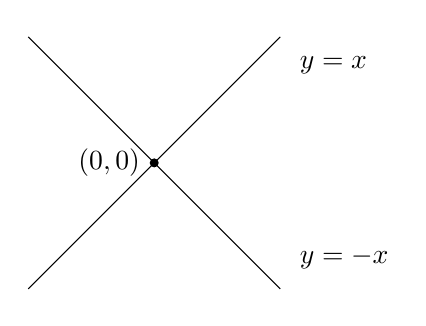
\begin{tikzpicture}
			  \draw (-1.6,-1.6) -- (1.6,1.6);
			  \draw (-1.6,1.6) -- (1.6,-1.6);
			  \node[circle, draw, fill=black, inner sep=1pt, label=left:{$(0,0)$}] at (0,0) {};
			  \node[label=above right:{$y=-x$}] at (1.6,-1.6) {};
			  \node[label=below right:{$y=x$}] at (1.6,1.6) {};
		  \end{tikzpicture}
		  \caption{Subvariedad $M = \{ y=x \cup y = -x \}$}
		  \label{figSubX}
	  \end{center}
  \end{wrapfigure}
  
  En este caso, vemos que $M = \{ y=x \cup y = -x \}$. No debería ser una subvariedad porque en el $(0,0)$ no es derivable (ver figura \ref{figSubX}). Intentaremos demostrarlo por reducción al absurdo.
  
  Supongamos que $M$ es una subvariedad. Entonces, según la definición (\ref{defSubDif})  existe un $U, (0,0) \in U$ y una aplicación  $\appl{G}{U\subset\real^2}{\real}$ con $U\cap M = \{G(x,y) = 0\}$. Entonces tendríamos que 
  
\[\rango DG(x,y) = 1, \forall(x,y) \in U \implies \rango \left(\dpa{G}{x},\dpa{G}{y}\right) = 1\]

Ahí tenemos dos casos, o bien que la primera componente no sea $0$ o que sea la segunda la que no es nula. Supongamos primero que $\dpa{G}{x}(0,0) \neq 0$. Podemos aplicar el Teorema de la unción implícita (\ref{TFImp}), que nos dice que podemos despejar $x = x(y)$. En este caso:

$U \cap M = \{x(y)^2-y^2 = 0\}$.

Si fijamos $y=\varepsilon$, entonces $x(\varepsilon) = \pm \varepsilon$ No es una función, lo que contradice el Teorema de la función implícita, y por lo tanto es imposible que $\dpa{G}{x}(0,0) \neq 0$. Análogamente, tampoco puede cumplirse que $\dpa{G}{y}(0,0) \neq 0$.

Hemos demostrado por lo tanto que no puede existir una función que defina esto como subvariedad diferencial. Este es el ejemplo de que cualquier objeto que tenga autointersección no puede ser subvariedad.

\paragraph{7)} $M = \{(x,y) \in \real^2 \tq x^2-y^2 = 0, y\ge 0\}$

Vamos a suponer que existe una función $F \in C^1$ que representa ese objeto (que viene definido por 2 condiciones). $M = \{F(x,y) = 0\}$ para alguna $F$.

Condición de rango: $\left(\dpa{F}{x},\dpa{F}{y}\right) \neq (0,0)$.
 Condición de rango: $\left(\dpa{F}{x},\dpa{F}{y}\right) = (0,0), x=y=0$.

 Vamos a ver si es subvariedad o no. En este caso intuimos que no debería serlo. Volvemos a demostrar por reducción al absurdo:

 Supongamos que $M$ es subvariedad, entonces $\exists G(x,y)$ tal que $\appl{G}{U\subset\real^2}{\real}, U \cap M = \{G(x,y) = 0\}$

 Supongamos $\displaystyle \dpa{G}{x}\neq 0$. Entonces tenemos \[ M\cap U = \{y(x)^2 - y^2 = 0\} \]

 Si fijamos $x=\varepsilon \implies y(x) = \abs{\varepsilon}$, pero esto quiere decir que $G \notin C^1$. De forma análoga con la segunda coordenada, vemos que $M$ no es una subvariedad.

\paragraph{8)} Nos quitamos el punto conflictivo del caso anterior, el $(0,0)$.

$N = \{(x,y)\in \real^2 \tq x^2-y^2 = 0, y>0\}$

La lógica nos dice que este caso si debería ser subvariedad diferencial:  la definición de la función es local, y siempre podremos encontrar un entorno que no incluya el 0, que es el punto problemático.

Comprobamos que efectivamente el rango de $\nabla F$ es máximo $\forall (x,y)\in \real^2$ y por lo tanto $M$ es una subvariedad.

\subsection{Subvariedades y parametrizaciones}
\paragraph{Ejemplo} Superficie en $\real^3$ parametrizada: $S = \{\Phi(u,v) = (x(u,v),y(u,v),z(u,v))\}$.

A la hora de trabajar con superficies parametrizadas, nos interesaría poder definir una especie de función inversa que nos permita hacer cambios en el plano y llevarlos a la superficie o al reves, pero... ¡tienen dimensiones distintas! La esperanza que nos queda es que la superficie parametrizada tiene dimensión 2, igual que el plano.

\begin{defn}[Homeomorfismo] \label{defHomeomorfismo}
Sea $\appl{\Phi}{\Omega\subset\real^N}{\real^{N+K}}, \Omega$ abierto.

$\Phi$ es un \emph{homeomorfismo} sobre su imagen $\dimplies $ la restricción $\appl{\Phi}{\Omega}{\Phi(\Omega)}$ es continua y tiene una inversa continua,
es decir, \[\exists \appl{\Psi}{\Phi(\Omega)}{\Omega} \tlq 
\left\{ \begin{array}{cc} 
\Psi(\Phi(\gor{u})) = \gor{u}, &\forall \gor{u} \in \Omega\\ 
\Psi(\Phi(\gor{x})) = \gx, &\forall \gx \in \Phi(\Omega)
\end{array}\right.\]

\paragraph{Definición 1)}
Dado un $\displaystyle x_0 \in \Phi(\Omega) \implies \forall \varepsilon >0, \exists \delta>0 \tlq$ 

si $\begin{array}{lc}
\norm{\gx-\gor{x_0})} < \delta \implies \norm{\Psi(\gx)-\Psi(\gor{x_0})}<\varepsilon\\
\gx \in \Phi(\Omega)
\end{array}$

\paragraph{Definición alternativa de continuidad}
Si $\{X_n\}\subset\Phi(\Omega), \gor{X_n} \rightarrow \gor{x_0}\in\Phi(\Omega) \implies \Psi(\gor{X_n}) \rightarrow \Psi(\gor{x_0})$

\end{defn}

\subsubsection{Ejemplos}


\paragraph{Ejemplo 1}

\[\appl{\sigma}{[0,2\pi)}{\real^2}\]
\[t \rightarrow \sigma(t) = (cos(t),sen(t))\]

Inversa: $\Psi(x,y) = t$ ángulo de la representación en polares.

Vamos a estudiar el problema de la continuidad:

Tomamos $\{(X_n,Y_n)\}$ con $x^2+y^2 = 1 \tlq (x_n,y_n) \convs (1,0)$

Si $\Psi$ es continua, debe ser $\Psi(x_n,y_n) \convs (1,0) = 0$. En este caso no es continua porque:

Si tomamos \begin{align*}
P_n &= \left(cos\left(2\pi - \frac{1}{n}\right), sen\left(2\pi - \frac{1}{n}\right) \right)\\
P_n &\convs (1,0)\\
\Psi(P_n) &= 2\pi - \frac{1}{n} \convs 2\pi\neq\Psi(1,0)
\end{align*}

\paragraph{Ejemplo 2}

\[\appl{f}{(0,1)\subset\real}{\real^2}\]
\[t \rightarrow f(t) = (t,g(t)), \text{continua, con inversa continua}\]

Vamos a definir la  inversa:
\[P\in f(0,1) \implies P(x,g(x)) \text{Para algún } x\in(0,1)\]
$P = (x,g(x))$

\[\Psi(P) = t \in (0,1) \tlq f(t) = (x,g(x)) \implies t = x\]
Vamos a estudiar la continuidad:
\[\{P_n\} \subset f(0,1), P_n \rightarrow P \in f(0,1)\]
\[P_i = (x_i,g(x_i)), \text{ para algún } i \in (0,1)\]
\[P_n \convs P_0 \dimplies (x_n,g(x_n)) \rightarrow (x_0,g(x_0)) \implies x_n (= \Psi(P_n)) \rightarrow x_0 (=\Psi(P_0)) \]

\obs ¿La gráfica de una función es homeomorfismo sobre su imagen?
\paragraph{Ejemplo 3}
\[\appl{\sigma_3}{(0,4\pi)}{\real^2}\]
\[t \rightarrow \sigma(t) = (cos(t),sen(t))\]
No es inyectiva $\implies \nexists \Psi$.

\paragraph{Ejemplo 4: Circunferencia}
\[\appl{\sigma_4)}{(0,2\pi)}{\real^2}\]
\[t \rightarrow \sigma(t) = (cos(t),sen(t))\]
La diferencia con el ejemplo 1, es que es cerrado.

Hay que percatarse de que la tangente no es inyectiva, entonces... la inversa es algo más complicada que $\arctan$, así que vamos a definirla a trozos siguiendo el esquema de la figura \ref{imgCirc_2}.

\begin{figure}[hbtp]
\begin{center}
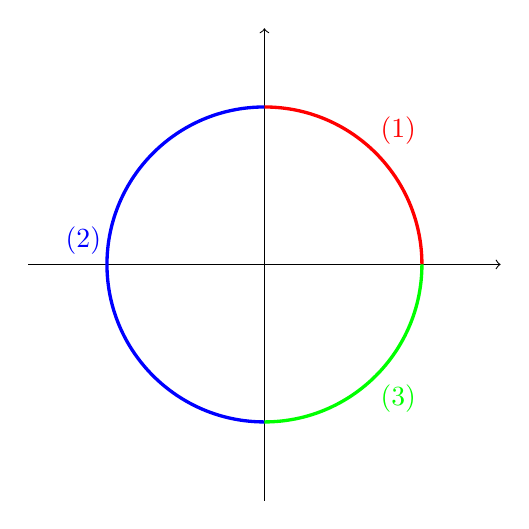
\begin{tikzpicture}[scale=1]
% Ejes
\draw[->] (-3,0) -- (3,0);
\draw[->] (0,-3) -- (0,3);

% Partes de la circunferencia
\draw[very thick,red] (2,0) arc (0:90:2);
\draw[very thick,blue] (0,2) arc (90:270:2);
\draw[very thick,green] (0,-2) arc(270:360:2);

% Etiquetas
\node[red] at (1.7, 1.7) {(1)};
\node[blue] at (-2.3, 0.3) {(2)};
\node[green] at (1.7, -1.7) {(3)};
\end{tikzpicture}
\caption{Circunferencia definida en tres trozos}
\label{imgCirc_2}
\end{center}
\end{figure}


\[\Psi(x,y) =
\begin{cases}
\arctan\left(\frac{y}{x}\right) & (x,y)\in 1\\
\arctan\left(\frac{y}{x}\right) + \pi & (x,y) \in 2\\
\arctan\left(\frac{y}{x}\right)+2\pi& (x,y) \in 3
\end{cases}
\]

Hay que estudiar la continuidad en $(0,-1)$ y en $(0,1)$.

\subparagraph{Continuidad en (0,1)}

Tomamos $\{P_n\} \rightarrow (0,1), P_n \in S_1$

Queremos probar que $\Psi(P_n) \rightarrow \Psi(0,1) = \frac{\pi}{2}$.

Ejercicio para el lector: 
Sucesiones que se acercan por la derecha o por la izquierda y comprobar que vale lo que tiene que valer.		

\paragraph{Ejemplo 5: Lemniscata}

\begin{figure}[hbtp]
\begin{center}
\begin{tikzpicture}[scale=2,declare function={
	lemnx(\x)=2.5*cos(\x) / ( sin(\x)^2+ 1);
	lemny(\x)=3*sin(\x) * cos(\x) / ( sin(\x) ^2 + 1;
	}]

% Ejes
\draw[->] (-3,0) -- (3,0);
\draw[->] (0,-2) -- (0,2);

% La curva
\draw[gray,domain=-90:270,samples=200] plot ({lemnx(\x)}, {lemny(\x)});

% Sucesión 1
\foreach \x in {-86,-82,...,-66}
\node[circle, red, draw,inner sep=2pt] at ({lemnx(\x)}, {lemny(\x)}) {};

% Sucesión 2
\foreach \x in {72,76,...,108}
\node[rectangle, blue, draw,inner sep=2pt] at ({lemnx(\x)}, {lemny(\x)}) {};

% Sucesión 3
\foreach \x in {242,246,...,266}
\node[diamond, orange, draw,inner sep=2pt] at ({lemnx(\x)}, {lemny(\x)}) {};

% Puntos t = 0, t=π
\node[label=above right:$t\eq 0$, draw, fill=white,circle, inner sep=2pt] at (2.5,0) {};
\node[label=above left:$t\eq \pi$, draw, fill=white,circle, inner sep=2pt] at (-2.5,0){};

% Flechas para indicar hacia donde va la t.
\foreach \x in {-45,44,134,224}
\draw[-angle 90] ({lemnx(\x)},{lemny(\x)}) -- ({lemnx(\x + 1)},{lemny(\x +1)});

% Etiquetas de las sucesiones.
\node[label={[red]below:(1)}] at ({lemnx(-66)},{lemny(-66)}) {};
\node[label={[blue]above:(2)}] at ({lemnx(72)},{lemny(72)}) {};
\node[label={[orange]above:(3)}] at ({lemnx(242)},{lemny(242)}) {};
\end{tikzpicture}
\caption{Curva Lemniscata}
\end{center}
\end{figure}

La parametrización es \[\sigma_5 (x(t),y(t)) = \left(\frac{\cos(t)}{\sin^2(t)+1},\frac{\sin(t)\cos(t)}{\sin^2(t)+1}\right), t\in \left(\frac{-\pi}{2},\frac{3\pi}{2}\right)\]

Al origen podemos acercarnos de distintas formas:

\begin{itemize}
\item Cuando $t \to - \frac{\pi}{2}$, nos acercamos por la sucesión 1 (desde abajo a la derecha).
\item Cuando $t \sim \frac{\pi}{2}$, nos acercamos por la sucesión 2 (la mitad de la curva, de arriba-derecha a abajo-izquierda).
\item Cuando $t \to \frac{3\pi}{2}$, nos acercamos por la sucesión 3 (desde arriba a la izquierda)
\end{itemize}

Sea $\{P_n\}\subset \sigma_5(t) \rightarrow (0,0)$.

Podemos tomar la sucesión $\{P_n\} = \{P_1,P_2,P_3,...\}$ cada uno en una región (1,2,3 ciclicamente).

\[\Psi(P_n) \begin{cases}
\in 3 & \text{ si }n \text{ es múltiplo de }3\\
\in 2 & \text{ si } n\equiv 2\ mod \ 3\\
\in 1 & \text{ si } n \equiv 1\ mod \ 3
\end{cases}\]

Por tanto $\nexists \displaystyle \lim_{n\rightarrow \infty} \Psi(P_n)$

\begin{remark} A pesar de que hemos demostrado que $\sigma$ es continua e inyectiva, esto no garantiza que la inversa sea continua.\end{remark}

\subsection{Parametrizaciones}

\paragraph{Objetivo} definir "parametrización".

\subparagraph{Ejemplo 1} Curva parametrizada en $\real^3$

$\Gamma = \{\sigma(t) = (x(t),y(t),z(t)), t \in (a,b)\}$

Queremos excluir:
\begin{itemize}
\item Picos (valor absoluto. FOTO) 

Basta con imponer: $\sigma \in C^1 \y (x',y',z') \neq (0,0,0)$

\item Auto-intersecciones o Lemniscata (que no se auto-intersecciona pero por poquito) 

Basta imponer $\sigma$ sea un homeomorfismo sobre su imagen.

\end{itemize}

\paragraph{Ejemplo 2} Superficies de parametrización en $\real^3$.

\[S = \{\Phi(u,v) = (x(u,v),y(u,v),z(u,v)), (u,v)\in D\}\]

Queremos evitar:

\begin{itemize}
\item Cono, tienda de campaña
$Rango \begin{pmatrix}
T_u \rightarrow\\
T_v \rightarrow
\end{pmatrix} = 2 \implies $ Podemos calcular plano tangente
\item Autointersección
Aquí sí tenemos rango máximo, asíque impondremos la condición de homeomorfismo sobre su imagen.
\end{itemize}

Ya tenemos todo lo necesario para definir parametrización:

\begin{defn}[Parametrización\IS local] \label{defParametrizacion}
Diremos que $\appl{\Psi}{\omega \subset \real^N}{\real^{N+K}}, \Psi \in C^1(\omega)$, es una parametrización local $\dimplies \left\{ \begin{array}{c}
 rango D\Psi = n \text{ máximo}\\
 \Psi \text{ es un homeomorfismo sobre su imagen}
\end{array}\right.$
\end{defn}



\subsubsection{Repaso de coordenadas cilíndricas y esféricas.}
\paragraph{Ejemplos}

\index{Helicoide}\label{Helicoide}
El \textbf{helicoide} es una función $\Phi$ de dos variables, que crea una superficie helicoidal (escalera de caracol) en el espacio, tal que 

\begin{align*} \appl{\Phi}{\real^2 &}{\real^3} \\
 (s,t) &\longmapsto \Phi(s,t) = (s\cos t, s\sin t, t) \end{align*}
 
 \easyimg{CALII/Helicoide.png}{El helicoide}{lblHelic}

En general, una superficie parametrizada es una aplicación $\Phi$ de la siguiente forma:

\begin{align*} \appl{\Phi}{\Omega \subset \real^2 &}{\real^3} \\
 (s,t) &\longmapsto \Phi(s,t) = (x(s,t), y(s,t), z(y,t)) \end{align*}

\index{Paraboloide}
Por ejemplo, el \textbf{paraboloide} se puede definir como una superficie parametrizada \[\Phi(x,y) = (x,y,x^2+y^2)\].

\index{Cilindro}
Otro ejemplo es el \textbf{cilindro} de radio 2. Para parametrizarlo, usamos coordenadas polares de la siguiente forma:

\[ \Phi(t,z) = (2\cos t, 2\sin t, z)\;\;t\in [0, 2\pi],\;\; z\in \real \]

\index{Esfera}
Si queremos hacer la \textbf{esfera} de radio $R$, en la parametrización usamos dos parámetros (longitud y latitud)

\[ \Phi(\theta, \phi) = (R\sin\phi\cos\theta, R\sin\phi\sin\theta, R\cos\phi)\;\; \theta\in[0,2\pi],\;\;\phi\in[0, \pi] \]

\index{Toro}
El \textbf{toro} (una especie de flotador) se produce al girar una circunferencia de radio $R_1$ en el plano $XZ$ con el centro sobre el eje $X$ a $R_2$ del origen alrededor del eje $Z$.

\[ \Phi(\theta, \phi) = ((R_2+R_1\cos\phi)\cos\theta,(R_2+R_1\cos\phi)\sin \theta,R1\sin \phi)\;\; \theta, \phi \in [0, 2\pi] \]

 \easyimg{CALII/Toro.png}{Toro}{lblToro}
\paragraph{Parametrización de superficies de revolución}
\index{Superficie!de revolución}

Dada una función $\appl{f}{\real}{\real}$, la superficie de revolución que surge al rotar esta función sobre el eje z es la siguiente

\begin{align*} z(r,\theta) &= f(r) \\
x(r,\theta) &= r \cos \theta \\
y(r,\theta) &= r \sin \theta \end{align*} 

\paragraph{Coordenadas cilíndricas}
\index{Coordenadas!cilíndricas}
Dado un punto $P$, sus coordenadas cartesianas son $(x,y,z)$. Entonces, sus coordenadas cartesianas son $(r,\theta, z)$, donde $r\in [0,\infty)$, $\theta \in [0,2\pi]$ y $z\in \real$. La correspondencia es la siguiente:

\begin{align*}
x &=r \cos \theta \\
y &= r \sin \theta \\
z &= z
\end{align*}

Geométricamente, $z$ es la altura de $P$. Haciendo la proyección del punto sobre el plano $xy$, $r$ es la distancia de la proyección al origen y $\theta$ el ángulo del eje $X$ con la recta que une el origen y la proyección del punto.

\paragraph{Coordenadas esféricas}
\index{Coordenadas!esféricas}
Las coordenadas esféricas de un punto $P$ son $(\rho, \theta, \phi)$, donde $\rho \in [0, \infty)$, $\theta\in [0, 2\pi]$, $\phi \in [0, \pi]$. La correspondencia con coordenadas cartesianas es

\begin{align*}
x&=\rho \cos \theta \sin \phi \\
y&= \rho \sin \theta \sin \phi \\
z &= \rho \cos \theta
\end{align*}

Geométricamente, $\rho$ es la distancia de $P$ al origen, $\theta$ es el ángulo que forman el eje $X$ y la recta que une $P$ y el origen, y $\phi$ es el ángulo que forman el eje $Z$ y esa misma recta.

\paragraph{Usos de coordenadas esféricas y cilíndricas}

En las coordenadas cilíndricas, si mantenemos constante un parámetro y variamos los otros dos obtenemos varias superficies:

\begin{itemize}
\item Si $r$ constante, tenemos un cilindro. \index{Cilindro}
\item Si $\theta$ constante, tenemos un semiplano. \index{Semiplano}
\item Si $z$ constante, tenemos un plano horizontal. \index{Plano}
\end{itemize}

Lo mismo ocurre con las coordenadas esféricas:

\begin{itemize}
\item Si $\rho$ constante, tenemos una esfera. \index{Esfera}
\item Si $\theta$ constante, tenemos un semiplano.\index{Semiplano}
\item Si $\phi$ constante, tenemos un cono. \index{Cono}
\end{itemize}

\subsubsection{Ejemplos}

\subparagraph{Esfera en $\real^3$}
 $\Phi_{1,2}(x,y) = (x,y,\pm \sqrt{1-x^2-y^2})$. Esta \emph{"carta de parametrización"} nos deja sin definir el ecuador. Para ello tenemos que definir más \emph{cartas de parametrización} \index{Carta de parametrización}
 
 Estas cartas son expresando x,y en función de las otras 2. En total hacen falta 3 parametrizaciones.
 
 \subparagraph{Existe} otra manera de parametrizar, la proyección estereográfica.  
 \index{Proyección \IS estereográfica}

El dibujo de la proyección es:

\begin{tikzpicture} % "THE GLOBE" showcase
%Definición de constantes:
\def\R{2.5} % sphere radius
\def\angEl{15} % elevation angle
\def\angAz{-105} % azimuth angle
\def\angPhi{-40} % longitude of point P
\def\angBeta{19} % latitude of point P


%Ecuador
\DrawLatitudeCircle[\R]{0} 

\pgfmathsetmacro\H{\R*cos(\angEl)} % distance to north pole

\tikzset{xyplane/.estyle={cm={cos(\angAz),sin(\angAz)*sin(\angEl),-sin(\angAz),
                              cos(\angAz)*sin(\angEl),(0,0)}}}


\LongitudePlane[xzplane]{\angEl}{\angAz}
\LongitudePlane[pzplane]{\angEl}{\angPhi}
\LatitudePlane[equator]{\angEl}{0}

%% draw xyplane and sphere

\fill[ball color=white] (0,0) circle (\R); % 3D lighting effect
\draw(0,0) circle (\R);
\draw[xyplane] (-2*\R,-2*\R) rectangle (3.2*\R,2.8*\R);

\coordinate (O) at (0,0);

\coordinate[mark coordinate] (N) at (0,\H);
\coordinate[mark coordinate] (S) at (0,-\H);

\path[pzplane] (\angBeta:\R) coordinate[mark coordinate] (P);
\path[pzplane] (2.75*\R,\R) coordinate (PE);
\path[xzplane] (0,0) coordinate (XE);
\path (PE) ++ (0,0) coordinate (Paux); % to aid Phat calculation
\coordinate[mark coordinate] (Phat) at (intersection cs: first line={(N)--(P)},
                                        second line={(S)--(Paux)});

\coordinate[mark coordinate] (P1) at (-2,-5/3);

\coordinate[mark coordinate] (P2) at (4,2/3);

\DrawLatitudeCircle[\R]{-1} % equator
\draw[xyplane,<->] (4*\R,0) node[below] {$u$} -- (0,0) -- (0,2.4*\R)
    node[right] {$v$};
\draw[->] (0,-\H) -- (0,1.6*\R) node[above] {$z$};

\draw[dashed] (P) -- (N) +(0.3ex,0.6ex) node[above left] {$\mathbf{N}$};
\draw (P) -- (Phat) node[above right] {$\mathbf{\hat{P}}$};
\path (S) +(0.4ex,-0.4ex) node[below] {$\mathbf{S}$};
\draw[->] (O) -- (P) node[above right] {$\mathbf{P}$};
\draw[blue] (P1) -- (P2) node[below right] {$\mathbb{X}\left(u,\frac{u-2}{3}\right)$};	

\path (P1) node [above left] {$\left(-2,\frac{-5}{3},0\right)$};
\path (P2) node [left] {$\left(4,\frac{2}{3},0\right)$};

\draw[red,name=lineP1N] (P1) -- (N);
\draw[red,name=lineP2N] (P2) -- (N);


\end{tikzpicture}


La imagen formada será la circunferencia que contenga la intersección (que ya no he sabido dibujar) de cada línea roja con la esfera y las 2 intersecciones (que tampoco he sabido dibujar) de la recta azul que es $\mathbb{X}\left(u,\frac{u-2}{3}\right)$.

 
 
 \[(u,v) \in \real^2 \rightarrow (u,v,0) \rightarrow r\equiv (0,0,R) + t(u,v,-R) = (tu,tv,R(1-t)\]
 Imponiendo $\underbrace{P}_{r(t_0)} \equiv r\cap S$ tenemos: \[(t_0u)^2+(t_0v)^2 + R^2(1-t)^2 = R^2 \rightarrow ... \rightarrow t_0 = \frac{2R^2}{u^2+v^2+R^2}\]
 
 Conclusión: \[P = (tu,tv,R(1-t) = \frac{2R^2}{u^2+v^2+R^2}u,\frac{2R^2}{u^2+v^2+R^2}v,\frac{R(u^2+v^2-R^2)}{u^2+v^2+R^2} = \Phi(u,v)\].
 
 Vemos que $\Phi\in C^1, \Phi(\real^2) = S_R-\{(0,0,R)\}$ ¿Es una parametrización?
 
 Hay que comprobar \begin{itemize}
 \item rango $D\Phi$ máximo. (Se deja como ejercicio para el lector)
 \item $\Phi$ es homeomorfismo sobre su imagen, es decir, ¿Existe una inversa continua? 
 
 \emph{Inversa}
 Dado $(x,y,z)$ queremos despejar $(u,v)$.
 
 Idea: $(u,v,0)$ es la intersección de la recta que unie $(x,y,z)$ con $(0,0,R)$ y el plano $z=0$.
 
 Recta: $s(t) = (tx,ty,R+t(z-R))$.
 
 Punto de corte con el plano $z=0$: El punto de corte tendrá coordenada tercera = 0, es decir: 
 $R+t(z-R)$
 
 Buscamos $t_0$ tal que $R+t_0(z-R)=0 \dimplies t_0=\frac{R}{R-z}$.
 
 Sustituyendo en la recta obtenemos: $u = t_0x, v=t_0y$
 
 Si calculamos $\Phi^{-1}(x,y,z) = \left(\frac{Rx}{R-z},\frac{Ry}{R-z}\right)$. Esta inversa es continua en $Img(\Phi(\real^2)) \equiv \{Esfera - \{(0,0,R)\}\}$  (El punto (0,0,R) no está incluido, por definición, en la imagen).
 
 \end{itemize}
\subsection{Teoremas de las subvariedades}
\begin{theorem}\label{thmSubvariedades}
Los siguientes enunciados son equivalentes:
\begin{itemize}
\item[1] $M$ es una subvariedad diferenciable n-dimensional en $\real^{N+K}$. \label{eq_1}
\item[2] $\forall \gor{a} \in M $ existe una parametrización local $\appl{\Phi}{\omega\subset \real^N}{\real^{N+K}}$ con $\gor{a}\in \Phi(\omega)$\label{eq_2}
\item[3] $\forall \gor{a} \in M$ existe un abierto $V\subset \real^{N+K}, \gor{a}\in V$ y una aplicación 
\label{eq_3}
\[\appl{\Psi}{V}{\real^{N+K}}, \Psi\ \text{difeomorfismo} \tlq \Psi = (\Psi_1,...,\Psi_n,\Psi_{n+1},...,\Psi_{n+k})\]
Si $\gx \in V\cap M \implies$
\[\Psi_{n+1}(\gx) = ... = \Psi_{n+k}(\gx) = 0\]
\end{itemize}
\end{theorem}
 
 \paragraph{Observación 1:} En \ref{eq_2}.2, llamaremos \textbf{carta local}\index{Carta!local} al conjunto definido por la fórmula y el dominio, $(\Phi,\omega)$. El conjunto de todas las cartas locales que definen una subvariedad se llama Atlas.
 
 \subparagraph{Ejemplo:} 
 
 La proyección estereográfica tiene 2 cartas, la del polo norte (que excluye ese punto) y la del polo sur.
 
 \paragraph{Observación 2:} $\ref{eq_1}.1 \dimplies \ref{eq_2}.2$. Si tenemos una subvariedad dada como conjunto de nivel la podemos parametrizar (y viceversa).
 
\begin{defn}[Difeomorfismo]
$\Psi$ es un difeomorfismo $\dimplies \Psi\in C^1,\exists \Psi^{-1}, \tlq \Psi^{-1}\in C^1$
\end{defn}
 


\begin{proof}
Esquema: $1\implies 2, 2\implies 3, 3 \implies 1$

\paragraph{1 $\implies$ 2\\}

Sea $\ga \in M, \exists U\subset\real^{N+K}$ abierto con $\ga \in U$ y una función $\appl{F}{U\subset \rnk}{\rk}, F\in C^1(U), \tlq U\cap M = \{\gx \in U\tq F(\gx) = \gor{0}\}$. Además $DF$ tiene rango máximo (K). 

Queremos demostrar que existe una parametrización $\Phi$.
\subparagraph{Permutando} el orden de las variables, suponemos que el menor de orden $K$ con determinante no nulo corresponde con las $K$ últimas variables. 

Por el teorema de la función implícita, $F(x_1,...,x_n,x_{n+1},...,x_{n+k}) = \gor{0}$, con $x_{n+1},...,x_{n+k}$ despejable en función de las $\{x_i,i=1,...,n\}$ en un entonro de $\gor{a}$.

Es decir: existen $\omega\subset \real^N, \omega'\subset\rk$ abiertos tales que $\gor{a}\in \omega \times \omega'$ y una función $\appl{g}{\omega\subset\real^N}{\omega'\subset\rk}$ de manera que
$$\left\{\begin{array}{c}
g(a_1,...,a_n) = (a_{n+1},...,a_{n+k})\\
F(\gx,g(\gx)) = \gor{0}, \forall \gx \in \omega\end{array}\right.$$

Idea: la parametrización es $\Phi (\gx) = (\gx,g(\gx))$

Vamos a comprobar las condiciones:
\begin{itemize}
\item $\Phi \in C^1$. Por el teorema de la función implícita, tenemos que $\Phi$ es diferenciable (porque $F$ y $g$ lo son).
\item \[D\Phi = ... = 
\begin{pmatrix}
Id_{n \times n}\\
\hline
Dg
\end{pmatrix}\] con rango máximo.
\item ¿Homeomorfismo sobre su imagen? $(x,y)\in M$ en un entorno de $\ga \in \omega\times\omega'$ En ese entonrno $y=g(\gx)$.
\end{itemize}
Es decir, $(x,y) = (x,g(x)) \xrightarrow{\Phi}) \gx \xrightarrow{\Phi^{-1}} (x,g(x)) = (x,y) $. También $\inv{\Phi}(x,y) = x, \forall(x,y)\in (\omega\times\omega') \cap M$ Continua.


\paragraph{2 $\implies$ 3} Vamos a emplear un argumento como el de la demostración del segundo teorema del rango. \ref{TR2}

Buscamos: 
\begin{align*}
\appl{\Phi}{\rnk}{\rnk} \tlq \Phi(V\cap M) = (\ast &,0)\\
&\uparrow\\
k \text{ últimas coor} & \text{denadas}
\end{align*}
Siendo $\Phi$ un difeomorfismo.

\paragraph{Sabemos:} existe una parametrización local $\appl{\Psi}{\real^N}{\rnk}$.
\begin{itemize}
\item $D\Psi$ rango máximo.
\item $\Psi$ homeomorfismo sobre su imagen.
\end{itemize}

\subparagraph{Idea:} Completar el número de variables

Definimos 
\begin{align*}
\appl{\alpha}{\omega\times\real^K \subset \real^N\times\real^K}&{\real^N\times\real^K}\\
(\gor{u},\gor{v})\longrightarrow &\alpha(\gor{u},\gor{v}) = \Psi(\gor{u}) + (\gor{0},\gor{v})\\
\gor{u} \in \real^N,\gor{v} \in \real^K, \Phi(\gor{u})\in \real^{N+K}
\end{align*}

\paragraph{Paso 2)} Aplicar el teorema de la función inversa (\ref{TFInv}) a $\alpha$.

\[D\alpha =
\left(
	\begin{array}{c|c}
		D\Psi_k  \rightarrow & 0\\
		\hline
		D\Psi_{n+i}  \rightarrow & I
	\end{array}
\right)
\]
Con $1\leq i \leq k,1\leq k \leq n$.

Por hipótesis, $rango(D\Psi)$ máximo. $\implies \exists \alpha^{-1}$.

\paragraph{Paso 3:} Comprobar que $\inv{\alpha}$ verifica las condiciones que buscamos.

Podría darse el caso de que en el conjunto $V\cap M$ hubiera 2 "trozos" de la subvariedad M, con lo que $\alpha$ no funcionaría bien. La condición de la parametrización eliminaba este caso.

Falta comprobar la condición de difeomorfismo, que se da porque... ¿porqué?

\paragraph{3 $\implies$ 1}

\textbf{Sabemos:} Existe un difeomorfismo $\Psi$.

\textbf{Buscamos:} $\appl{F}{W\subset \rnk}{\real^K} \tlq \displaystyle \left\{\begin{array}{c}
M\cap W = \{F(\gx) = \gor{0}\}\\
rango(DF) = k \text{ (máximo)}
\end{array}\right.$

Tomamos $F(\gx) = (\Psi_{n+1}(\gx),...,\Psi_{n+k}(\gx))$

Entonces: $M\cap V = \{ \gx \tq F(\gx) = \gor{0}$.

Tenemos $DF = \begin{pmatrix}
D\Psi_{n+1} \rightarrow\\
\vdots\\
D\Psi_{n+k} \rightarrow
\end{pmatrix}$

$Rango(DF) = k$ por tener $\det D\Psi \neq 0$ por hipótesis.

\end{proof}

\paragraph{Consecuencias:}

\subparagraph{1)}
Si $M$ es una variedad diferenciable de dimensión $N$ en $\rnk$, entonces, reordenando las variables puede escribirse \textbf{localmente} como la gráfica de una función $C^1, \underbrace{M\cap U}_{(*)} = \{(\gx,g(\gx))\}$

$(*) \implies$ un trozo de la variedad.


\subparagraph{2)}

\begin{theorem}
Sea  $\appl{\gamma}{\omega\subset\real^N}{\rnk}, \gamma \in C^1, rg(D\gamma) = max, \gamma(\omega)\subset M$ subvariedad de dim n.

\textbf{Entonces:} $\gamma$ es una parametrización local.	
\end{theorem}

\textbf{Aplicación:} Si existe $\gamma \in C^1, rg(D\gamma) = n, \gamma(\omega)\subset M \ y \ \gamma
$ no es homeomorfismo sobre su imagen $\implies$ \textbf{M} no es subvariedad.

Pregunta: Verdadero o Falso:

¿Con encontrar una aplicación que no sea homeomorfismo basta para asegurar que M no es subvariedad?

\paragraph{3)\\}

La prueba de este teorema se deja como ejercicio para el lector.

\begin{theorem}
Sea M subvariedad diferenciable n-dimensional en $\rnk$.

Sean $\appl{\Phi_1}{U_1}{M} \ y \ \appl{\Phi_2}{U_2}{M}$ dos parametrizaciones locales con $\Phi_1(U_1)\cap \Phi_2(U_2)\neq \emptyset$

\textbf{Entonces:} $\appl{\inv{\Phi_1}\circ \Phi_2}{\real^N}{\real^N}, con \inv{\Phi_1}\circ \Phi_2 \in C^1$. Análogamente para $\inv{\Phi_2}\circ\Phi_1$
\end{theorem}

\section{Espacios tangentes}

Sea $M$ subvariedad n-dimensional en $\rnk$.

$T_{\gor{a}}M \leadsto$ espacio tangente a M en el punto $\gor{a}\in M$

Pero... ¿qué es un hiperplano tangente? El concepto no es tan simple como un plano tangente. El espacio tangente será el conjunto de todos los vectores tangentes a cada una de las curvas contenidas en la superficie. A partir de aquí buscaremos una forma más eficiente de construirlo (porque es imposible calcular todas y cada una de las curvas contenidas en la superficie).

\begin{defn}[Vector\IS tangente]
Si $\gx \in \rnk$ es tangente a M en $\gor{A} \in M \dimplies \exists \appl{\sigma}{(-1,1)}{\rnk}, \sigma \tlq \left\{\begin{array}{lc}
\sigma(t) \in M, \forall t\in (-1,1)\\
\sigma(0) = \gor{a}\\
\alpha'(0) = \gor{v}
\end{array}\right.$
\end{defn}
\begin{defn}[Espacio\IS tangente]
\[T_aM \equiv \{ \gor{v} \in \rnk \tq \gor{v} \text{ es tangente a M en }\gor{a}\}\]
\end{defn}

\obs Cualquier curva de la variedad la podremos ver como una curva en la proyección (con una parametriazación construida cuidadosamente)

\begin{theorem}
Sea $M$ subvariedad en $\real^M$, $N$ subvariedad en $\real^N$.
\[\appl{f}{\Omega\subset\real^M}{\real^N}, \tlq f(\Omega\cap M) \subset N, f\in C^1\]

Sea \[\left.\begin{array}{lc}
\gor{a} \in \Omega\cap M \\ 
\gor{v} \in T_aM
\end{array}\right\} 
\implies Df(\gor{a})\gor{v} \in T_{f(\ga)}N\]
\end{theorem}

Es decir, si tenemos una parametrización, la diferencial lleva tangentes en tangentes.

\begin{proof}
Sea $\gor{v} \in T_{\ga} M$
Entonces $\exists \appl{\alpha}{(-1,1)}{M} \tlq \left\{\begin{array}{c}
\alpha(0) = \ga\\
\alpha'(0) = \gor{v}
\end{array}\right.$
Tomamos $\beta = f \circ \alpha$ curva sobre $N$ 

tal que $\left\{\begin{array}{lc} \beta(0) = f(\alpha(0)) = f(\ga)\\ 
\beta'(0) = Df(\alpha(0))\cdot \alpha'(0) = Df(\ga)\gor{v}\end{array}\right.$ (Aplicando la regla de la cadena sin más.)
\end{proof}


\subsection{Caracterizaciones del espacio tangente}
\textbf{Caracterización 1)}
\begin{theorem}\label{thmCaractTangente1}

$M$ subvariedad n-dimensional en $\rnk$. $\ga \in M$

Entonces:

\begin{itemize}
\item $T_{\ga}M$ es un espacio vectorial n-dimensional
\item $M$ definida como $\{F = 0\}$. Entonces $T_{\ga} M = \ker(DF(\ga))$
\end{itemize}
\end{theorem}

\begin{proof}
$U\cap M =\{ \gx \in \rnk \tq F(\gx) = \gor{0}\}$ para alguna $\appl{F}{\rnk}{\real^N}, rg(DF) = max$

\[\appl{F}{U\cap M}{\gor{0}}\]

Entonces: $DF(\ga)$ lleva $T_a M$ al espacio $T_0\{\gor{0}\}$

Es decir: $DF(\ga)\gor{v} = \gor{0}, \forall \gor{v}\in T_{\ga} M$

Esto demuestra $T_{\ga} M \subset \ker DF(\ga)$

Como el rango es máximo, sabemos que $\ker(DF(\ga))$ tiene dimensión $n$.

La idea a aplicar es encontrar $n$ vectores independientes en ese espacio tangente ¿Cómo vamos a encontrarlos? En el espacio de los parámetros tenemos n rectas independientes (los n ejes de coordenadas)

La parametrización nos lleva esas $n$ rectas en $n$ curvas. 

Por el teorema anterior, la diferencial lleva tangentes en tangentes, es decir, aplicando la diferencial a los vectores directores de las $n$ rectas encontramos los vectores tangentes a las $n$ curvas. 

¿Cómo podemos saber que esos vectores son independientes? Porque la diferencial tiene rango $n$.

Acabamos de demostrar  $\ker DF(\ga) \subset $\{ espacio vectorial de dimensión n\} 

Si $T_{\ga} M$ contiene un espacio vectorial de dimensión $n$ y está contenido por el núcleo (espacio vectorial de dimensión $n$).
\end{proof}

\paragraph{Caracterización 2)}
\begin{corol}
\label{CaractSubv_2}
$M$ dada por una parametrización $\Phi$ tal que $\Phi(\gor{u_0}) = \ga$ 

Entonces $T_{\ga} M = \img D\Phi(\gor{u_0})$

\end{corol}


El teorema y el corolario son las 2 caracterizaciones del espacio tangente.

Pero también podemos definir el espacio tangente con una tercera caracterización:

\paragraph{Caracterización 3)} Como gráfica. Sea $\appl{f}{\real^N}{\real^{K}}$

\[M\equiv \left\{(\gu,f(\gu)),\begin{matrix}
(\gu,f(\gu))\in \rnk\\
\gu \in \Omega\subset\real^N\\
 \appl{f}{\real^N}{\real^K}\end{matrix}\right\} \]

Salvo reordenación de las variables.

Sea $p=(\ga,f(\ga))$ el punto en el que queremos calcular el hiperplano tangente a $M$.

La caracterización será
\[T_p(M) = \{(\gu,v)\in\real^N\x\real^{K} \tq v = Df(a) \gu\}\]

\obs la otra alternativa es definir la subvariedad como $M = \{(\gu)\in\real^k \tq f(\gu) = f(\ga)$

\begin{defn}
$M\subset\rnk$ subvariedad n-dimensional, $\ga \in M$

\begin{itemize}
\item Espacio tangente $T_{\ga}M$
\item Hiperplano tangente $T_{\ga}$ "trasladado" al punto $\ga$
\[\{\gx \in \rnk \tq \gx-\ga \in T_{\ga}M\}\]
\item Hiperplano normal $\equiv \{\gx\in\rnk \tq \gx -\ga \in (T_{\ga}M)^{\bot}\} = \{\gx \in \rnk \tq \pesc{\gx-\gor{a},\gor{v}} = 0, \forall \gor{v}\in T_{\ga}M\}$. El hiperplano normal es k-dimensional.
\end{itemize}
\end{defn}


\paragraph{Ejemplos:}

\subparagraph{1)}

$ M = \{(x,y) \in \real^2 \tq x^2+y^2 = 1\}$.

\textit{Comprobación previa} Es una subvariedad porque...


Vamos a calcular \[T_{(a,b)}M = \ker \{\begin{pmatrix} 2x & 2y \end{pmatrix}\} =\]
\[ \{(u,v) \tq \begin{pmatrix}
2a & 2b
\end{pmatrix}\begin{pmatrix}
u\\v
\end{pmatrix} = 0\} = ... =  \{(u,v)\in \real^2 \tq \pesc{(a-0,b-0),(a,b)-(u,v)} = 0\].

El espacio tangente es el formado por todos los vectores perpendiculares al radio.

\subparagraph{Ejemplo 2: Toro (donut) en $\real^4$}

\[M = \{ (x,y,z,t)\in \real^4 \tq x^2+y^2 = 1, z^2+t^2 = 1\}\]
Vamos a calcular: $T_{(1,0,0,1)}M$

\textbf{Comprobación previa}...

Tenemos definida la variedad de forma implícita: $M = \{F = 0\}$ donde \[F(x,y,z,t) = (x^2+y^2-1,t^2+z^2-1)\]

\[DF = \begin{pmatrix}
2x&2y&0&0\\
0&0&2z&2t
\end{pmatrix}\]

En este caso tenemos $rg(DF) = 2, \forall (x,y,z,t)\in \real^4$. (El único punto que podría dar rango 0 es el origen, que en este caso no pertenece a la subvariedad)

Vamos con el espacio tangente:

\[T_{(1,0,0,1)}M = \ker DF (1,0,0,1) = \ker \begin{pmatrix}
2&0&0&0\\
0&0&0&2
\end{pmatrix} =\]
\[ \{ (\alpha_1,\alpha_2,\alpha_3,\alpha_4) \in \real^4 \tq \begin{pmatrix}
2&0&0&0\\
0&0&0&2
\end{pmatrix} \begin{pmatrix}
\alpha_1\\
\alpha_2\\ \alpha_3\\ \alpha_4
\end{pmatrix} = \begin{pmatrix}
0 \\
0
\end{pmatrix}\} \implies \left\{\begin{array}{cc}2\alpha_1 &= 0\\ 2\alpha_4 & =0\end{array}\right.\]

Hiperplano tangente:

\[
\begin{pmatrix}
1\\0\\0\\1
\end{pmatrix}
+ \alpha_2 \begin{pmatrix}
0\\1\\0\\0 	
\end{pmatrix}
+ \alpha_3
\begin{pmatrix}
0\\0\\1\\0
\end{pmatrix}, \alpha_2,\alpha_3 \in \real
\]

Y el hiperplano normal:

\[
\begin{pmatrix}
1\\0\\0\\1
\end{pmatrix}
+ \mu \begin{pmatrix}
1\\0 \\0\\0 	
\end{pmatrix}
+
\lambda
\begin{pmatrix}
0\\0\\0\\1
\end{pmatrix}, \lambda,\mu \in \real
\]

¿Una posible parametrización de esto?

\begin{align*}
\Phi : D \subset \real^2 \longrightarrow &\real^4\\
(u,v) \longrightarrow &\Phi(u,v) = (x,y,z,t) = \left(cos(u),sen(u),cos(v),sen(v)\right)\\
(u,v)\in (-\pi,\pi)\times(0,2\pi)
\end{align*}

¿¿Por qué $(u,v)\in (-\pi,\pi)\times(0,2\pi)$ y no $(u,v)\in (0,2\pi)\times(0,2\pi)$??

Porque el punto que tenemos $(1,0,0,1) \notin \img$. 

Vamos a calcular la el hiperplano tangente. Como tenemos una parametrización, calcularemos la imagen de la diferencial (\ref{CaractSubv_2})
\[T_{(1,0,0,1)}M = \img D\Phi\left(0,\frac{\pi}{2}\right)\]
\[D\Phi = \begin{pmatrix}
-sen(u) & 0\\
cos(u) & 0\\
0 & -sen(v)\\
0&cos(v)
\end{pmatrix}\]
\[D\Phi\left(0,\frac{\pi}{2}\right) = \begin{pmatrix}
0&0\\1&0\\0&-1\\0&0
\end{pmatrix}\]

Entonces el hiperplano tangente es:

\[\begin{pmatrix}
1\\0\\0\\1
\end{pmatrix} + u \begin{pmatrix}
0\\1\\0\\0
\end{pmatrix}
- v \begin{pmatrix}
0\\0\\1\\0
\end{pmatrix}
\]

Lógico y normal que nos de el mismo hiperplano tangente si estamos trabajando con el mismo objeto (desde una parametrización o desde un conjunto de nivel). ¿Cierto y verdad que sí?

\paragraph{Ejemplo 3: El toro en $\real^3$}
\index{Toro}

El \textbf{toro} (una especie de flotador) se produce al girar una circunferencia de radio $R_1$ en el plano $XZ$ con el centro sobre el eje $X$ a $R_2$ del origen alrededor del eje $Z$.

\[ \Phi(\theta, \phi) = ((R_2+R_1\cos\phi)\cos\theta,(R_2+R_1\cos\phi)\sin \theta,R1\sin \phi)\;\; \theta, \phi \in (0, 2\pi) \]

\easyimg{CALII/Toro.png}{Toro}{lblToro2}

¿Es $\Phi$ una parametrización? 
\begin{itemize}
\item Opción 1: Comprobar homeomorfismo sobre la imagen
\item Opción 2: Aplicar el teorema. Si el toro es una subvariedad $\implies \Phi$ parametrización.
\end{itemize}

Vamos con la opción 1:
\[\Phi(\alpha,\theta) = (x,y,z)\]
\[¿(\alpha,\theta) = \Phi^{-1} (x,y,z)?\]
\[z = rsen(\alpha) \implies \alpha = arcsen\left(\frac{z}{r}\right)\]
\[\frac{y}{x} = tg(\theta) \implies \theta = arctg \left(\frac{y}{x}\right)\]


%Revisar
Esto no es suficiente, porque $\appl{arcsen}{(-1,1)}{\left(\frac{-\pi}{2},\frac{\pi}{2}\right)}$ no toma todos los posibles valores. Lo mismo con la $\appl{arctg}{\real}{\left(\frac{-\pi}{2},\frac{\pi}{2}\right)}$

Tenemos que repetir el argumento de (\ref{imgCirc}) que ya hemos hecho para la $arctg$ vamos a repetirlo para el $arcsen$.

\begin{figure}[hbtp]
\begin{center}
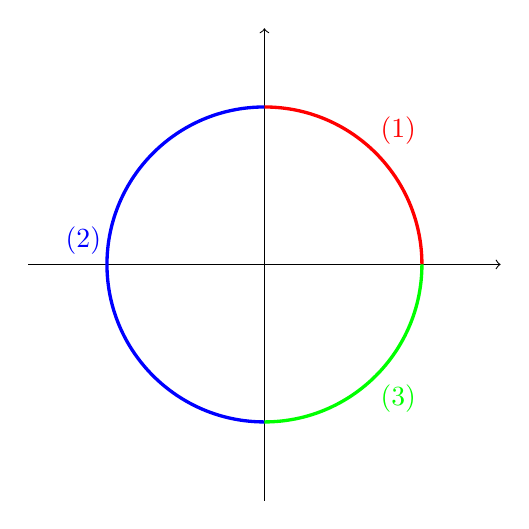
\begin{tikzpicture}[scale=1]
% Ejes
\draw[->] (-3,0) -- (3,0);
\draw[->] (0,-3) -- (0,3);

% Partes de la circunferencia
\draw[very thick,red] (2,0) arc (0:90:2);
\draw[very thick,blue] (0,2) arc (90:270:2);
\draw[very thick,green] (0,-2) arc(270:360:2);

% Etiquetas
\node[red] at (1.7, 1.7) {(1)};
\node[blue] at (-2.3, 0.3) {(2)};
\node[green] at (1.7, -1.7) {(3)};
\end{tikzpicture}
\caption{Circunferencia definida en tres trozos}
\label{imgCirc}
\end{center}
\end{figure}


\[f(x,y,z) =\left\{ \begin{matrix}
Si & (x,y,z) \in 1 &\implies &arcsen\left(\frac{z}{r}\right)\\
Si & (x,y,z) \in 2 &\implies &\displaystyle\frac{\alpha + arcsen\left(\frac{z}{r}\right)}{2} = \frac{\pi}{2}\\
Si & (x,y,z) \in 3 &\implies & \alpha = arcsen\left(\frac{z}{r}\right) + 2\pi
\end{matrix}\right.
\]

Ahora tenemos que estudiar la continuidad des esta función. (Ejercicio para el lector)


\subparagraph{$T_{\ga}M$}

En este caso (al tratarse de una diferencial) tendremos que hallar la imagen de $D\Phi$.

Ejercicio propuesto: $T_{\left(\frac{\pi}{2},\frac{\pi}{2}\right)}M$.


\begin{problem}[4.4]
Sea $\sigma(t) = \left( cos(t),sen(t),t^2(2\pi - t)^2\right), t \in [0,2\pi]$.
\solution
Siempre hemos hablado de parametrizaciones es espacios abiertos, para asegurar la condición de homeomorfismo en casos como este, en el que los puntos cerca de $0$, la inversa me los lleva a puntos lejanos si nos acercamos a $0$ por el $0$ o por el $2\pi$.

Posibles soluciones
\begin{itemize}
\item  Trabajar con el intervalo abierto, pero entonces... el punto $(1,0,0)$ que es el que nos piden no pertenece. ¿Cómo calcular el espacio tangente en $(1,0,0)$? Podríamos hacer los "límites laterales" y calcular el $T_{(1^{-},0,0)}M, T_{(1^{+},0,0)}$ por decirlo de alguna manera y si coinciden, ese tiene que ser el hiperplano tangente en el punto $(1,0,0)$.

\item Definir otro intervalo en el que trabajar. 

Con el $sen$ y $cos$ no tenemos problema porque son periódicas y podríamos trabajar en $\left(\frac{\pi}{2},\frac{\pi}{2}\right)$ pero con la tercera coordenada es más problemático porque no es periódica. Es de la forma:

%\easyimg{imgs/TercCoor.png}{TercCoor}{lblTercCoor}

Idea: 
\begin{itemize}
\item Escribir la extensión $2\pi$ periódica al intervalo $[-2\pi,2\pi]$.
\item Tomar $\tilde{\sigma}(t) = (cos(t),sen(t),\tilde{z}(t)), t\in (-\pi,\pi)$
\end{itemize}
\end{itemize}

\end{problem}

\section{Máximos y mínimos condicionados}

\begin{defn}[Extremo\IS condicional]
$\Omega\subset\real^n$, abierto, $\appl{F}{\Omega}{\real}$ y M subvariedad de $\real^n, M\subset \Omega$

\textbf{Definición:}

\begin{itemize}
\item $F$ alcanza en $\ga\in M$ un extremo local condicionado a $M \dimplies$ existe un abierto \[U\in\real^n\, con \, \ga\in U \tlq \left\{\begin{matrix} F(\gx) \leq F(\ga), \forall \gx \in U\cap M \\
F(\gx) \geq F(\ga), \forall \gx \in U\cap M \end{matrix}\right.\]
\end{itemize}

\end{defn}


\begin{theorem}[Teorema\IS de los multiplicadores de Lagrange] \label{thmMultLagrange}
$\appl{F}{\Omega\subset\rnk}{\real}, F\in C^1(\Omega)$.

M, variedad n-dimensional en $\rnk$. $\ga\in M$ extremo local de $F$ condicionado a M.

Supongamos que en un entorno de $\ga$:

$M = \{G = \gor{0}\} y \, rg(DG)=max$

\textbf{Entonces:} Existen $\lambda_1,...,\lambda_k \in \real$ tales que
\[\nabla F(\ga) = \sum \lambda_i \nabla G_i (\ga)\]
\end{theorem}

\begin{proof}
$\ga \in M$. Consideremos $T_{\ga}M = \ker [DG(\ga)]$

\[DG(\ga) = \begin{pmatrix}
\nabla G_1(\ga) &\longrightarrow \\
\nabla G_2(\ga) &\longrightarrow \\
\vdots\\
\nabla G_k(\ga) &\longrightarrow 
\end{pmatrix}\]

Sea $\gv \in T_{\ga M}$. Entonces $DG(\ga)\cdot\gv = \gor{0}\in\real^K$

Este producto es como \[\begin{pmatrix}
\pesc{\nabla G_1(\ga),\gv}\\
\pesc{\nabla G_2(\ga),\gv}\\
\vdots\\
\pesc{\nabla G_k(\ga),\gv}
\end{pmatrix}\]

Podemos concluir que $\nabla G_j(\ga)\perp T_{\ga} M \forall j=1,...,k$, es decir $\nabla G_j(\ga) \in (T_{\ga}M)^\perp,\forall j=1,...,k$

La condición de rango máximo nos asegura que 
\[\{\nabla G_i, i = 1,...,n\} \text{ es una base de } (T_{\ga} M)^\perp\]

Ahora solo falta probar que  $\gv \in T_{\ga} M \implies \nabla F(\ga)\perp\gv$, es decir $\nabla F(\ga) \in (T_{\ga} M)^\perp$.

\[\gv \in T_{\ga} M \implies \exists \appl{\alpha}{\real}{M} \alpha \in C^1, \alpha(0) = \ga, \alpha'(0) = \gv\]

Definimos $g(t) = F(\alpha(t))$

$F$ extremo en $\ga \implies g$ extremo en $t=0$.

\[ 0 = g'(0) = DF(\alpha(0))\cdot \alpha'(0) = \pesc{\nabla F(\alpha(0)),gv} = \pesc{\nabla F(\ga),gv}\]

Conclusión $ 0 = \pesc{\nabla F(\ga),gv} \implies \nabla F(\ga) \in (T_{\ga}M)^\perp$

\end{proof}


\paragraph{Ejemplos:}

\subparagraph{1)} $F(x,y) = x^2-y^2$. Sea $M = \{x^2+y^2 = 1\}$.

%Revisar. Falta pintar la circunferencia
%\easyimg{imgs/MCNSM.png}{Mapa de conjuntos de nivel de la silla de montar}{lblMCNSM}

%Si calculamos el máximo y el mínimo condicionados a la circunferencia de $R=1$ vemos que $\nabla F$ es paralelo al radio de la circunferencia, como consecuencia de la tangencia entre el conjunto de nivel y la subvariedad $M$. 

\begin{itemize}
\item $M$ es cerrado y acotado, es decir $M$ es compacto, $G^{-1}({0}) \equiv M, G(x,y) = x^2+y^2-1$
\item F continua
\end{itemize}

 $\implies$ se alcanza máximo y mínimo.


\textbf{Vamos con los multiplicadores.}

$\nabla F = (2x,-2y), \nabla G=(2x,2y)$

El sistema queda:

\[\left\{\begin{array}{ccc}
2x &=& \lambda 2x \\
2y &=& -\lambda 2y\\
x^2+y^2 &=& 1
\end{array}\right\}\]

Hay 2 posibles casos: $x=0$ e $y=0$

En el caso $y=0$

\[\left\{\begin{array}{ccc}2x&=&2x \lambda \\y&=&0\\x^2+0^2&=&1\end{array}\right\} \implies \left\{\begin{array}{cc}x=&\pm 1 \\ \lambda=1 \end{array}\right\}\]

Puntos críticos: $(1,0),(-1,0)$ con $F(\pm 1,0) = 1 \implies MAX$

En el caso $x = 0$.

\[ \left\{\begin{array}{ccc}
x &=& 0\\
-2y &=& \lambda 2y \\
y^2 &=& 1
\end{array}\right\}\dimplies
\left\{ \begin{array}{cc}
y &= \pm 1\\
\lambda &= -1
\end{array}\right\}\]

Puntos críticos: $(0,1),(0,-1)$, con $F(0,\pm 1) = -1 \implies MIN$

\paragraph{Ejemplo 2)} (Hoja 4, ejercicio 13)

Hallar los puntos críticos más cercanos al origen entre los contenidos en la curva
\[\Gamma = \left\{ \begin{array}{cc} x^2+xy+y^2-z^2-1&=0\\x^2+y^2-1&=0\end{array}\right.\]

En este caso: $M = \Gamma$ y tomamos $F(x,y,z) = x^2+y^2+z^2$ y $G(x,y,z) = (x^2+xy+y^2-z^2-1,x^2+y^2-1)$

\subparagraph{1) Compacidad}

$\Gamma$ es un conjunto cerrado porque las 2 ecuaciones definen un cerrado, y la intersección de 2 cerrados es un cerrado. Además está acotado porque e2 acota $x$ e $y$, y la e1 acota la z teniendo acotadas $x$ e $y$.

\subparagraph{2) Continuidad}

$F$ es continua.


Vamos con los multiplicadores:

\[
\left\{
\begin{array}{cl}
2x &= \lambda_1(2x+2y)+ \lambda_2 2x\\
2y &= \lambda_1(x+2y) + \lambda_2 2y\\
2z &= \lambda_1(-2z)\\
x^2+xy+y^2-z^2& = 1\\
x^2+y^2 &= 1
\end{array}\right\}\]
La tercera ecuación distingue 2 casos:
\[
\rightarrow
\left\{\begin{array}{cl}
Caso\, 1 &z=0\\
Caso\, 2 &\lambda_1 = -1\\
\end{array}\right.\]

\textbf{Caso 1:}

\[\left\{
\begin{array}{cl}
2x &= \lambda_1(2x+2y) + \lambda_2 2x\\
2y &= \lambda_1(x+2y) + \lambda_2 2y\\
x^2+xy+y^2& = 1\\
x^2+y^2 &= 1
\end{array}\right\}\]

De las últimas 2 ecuaciones vemos que $xy=0$. Distinguimos casos:

\[\left\{\begin{array}{ccc}
Caso\, 1.1& x=0 &\rightarrow y = \pm 1\\
Caso\, 1.2& y=0 &\rightarrow x = \pm 1
\end{array}\right\}\]

Tenemos 4 puntos críticos $P_1 = \{(1,0,0),(0,1,0),(-1,0,0),(0,-1,0)\}$ con $d[(x,y,z),(0,0,0)]=1, \forall (x,y,z)\in P_1$

\textbf{Caso 2:} (Podría darse el caso de que nos saliera la misma solución que en el caso 1. No preocuparse, es posible.)


\[\left\{\begin{array}{cc}
2x&= -(2x+y) + \lambda_2 2x\\
2y&= -(x+2y) + \lambda_1 2y\\
x^2+xy+y^2 -z^2 &= 1\\
x^2+y^2&=1
\end{array}\right\}\]

Restando las 2 ultimas ecuaciones nos dan que $xy = z^2 \neq 0 \implies x,y\neq 0$.

Multiplicando la primera y la segunda tenemos el sistema:

\[\left\{\begin{array}{cc}
2xy &= \left[-(2x+y)+\lambda_2 2x\right]y\\
2xy &= \left[-(x+2y)+\lambda_2 2y\right]x
\end{array}\right\} = \left\{\begin{array}{cc}
2xy+(2-\lambda_2) &= -y^2\\
2xy+(2-\lambda_2) & = -x^2\end{array}\right\}
\]

Sumando las ecuaciones tenemos:
\[\left\{\begin{array}{cc}
4xy(2-\lambda_2) &= - \underbrace{(y^2+x^2)}_{=1} = -1\\
4xy(2-\lambda_2)&= -1\end{array}\right\}\]

Si ahora las restamos tenemos \[\begin{array}{cc}x^2&=y^2\\x^2+y^2 &= 1\\ x\cdot y = z^2 &\implies sign(x)=sign(y) \end{array}\]

Llegamos a:

\[P_2 = \left\{
\left(\frac{1}{\sqrt{2}},\frac{1}{\sqrt{2}},\frac{1}{\sqrt{2}}\right),
\left(\frac{-1}{\sqrt{2}},\frac{-1}{\sqrt{2}},\frac{1}{\sqrt{2}}\right),
\left(\frac{1}{\sqrt{2}},\frac{1}{\sqrt{2}},\frac{-1}{\sqrt{2}}\right),
\left(\frac{-1}{\sqrt{2}},\frac{-1}{\sqrt{2}},\frac{-1}{\sqrt{2}}\right)
\right\}\] con $d[(x,y,z),(0,0,0)] = \frac{3}{2}, \forall (x,y,z)\in P_2$

\subsection{Clasificación de puntos críticos condicionados}

Sea $M$ una subvariedad de manera que $M=\{G = \gor{0}\}$ definida por un sistema de $k$ ecuaciones $G=(G_1,\dotsc,G_k)$ con $\rango DG = k$. Sea $P\in M$ un punto crítico de una función $F$ restringida a $M$. El teorema de los multiplicadores de Lagrange (\ref{thmMultLagrange}) nos dice que 

\[ \grad F(P) - \lambda_1 DG_1(P) - \dotsb -\lambda_kDG_k(P) = \gor{0} \]

donde los $\lambda_j$ son los multiplicadores. Definimos una función auxiliar 

\begin{equation} H(\gx) = F(\gx) - \lambda_1 G_1(\gx) - \dotsb - \lambda_k G_k(\gx)\label{eqClasAux} \end{equation}

con dos propiedades interesantes:

\begin{gather*}
\gx\in M\implies H(\gx) = F(\gx) \\
\grad H(P) = \gor{0} 
\end{gather*}

Para clasificar el punto crítico vamos a coger una curva dentro de la subvariedad y a componerla con $H$. Pasaremos a tener una función de una variable y ahí veremos en qué condiciones tenemos un máximo o un mínimo.

Tomamos una curva $\alpha\in C^1$ tal que 
\begin{gather*}
\alpha(0) = P \\
\alpha(t) \in M\; \forall t \\
\alpha'(0) = \gv
\end{gather*}

Estudiamos $g(t) = H(\alpha(t)) = F(\alpha(t)$. Entonces

\[ g'(t) = \pesc{\grad H(\alpha(t)),\alpha'(t)} \]

y entonces \[ g'(0) =\pesc{\grad H(P),\gv} = 0\]

Como $F$ tiene un punto crítico condicionado en $P$, entonces $g$ tiene un punto crítico en $t = 0$. Determinar el carácter del punto crítico condicionado es lo mismo que determinar el carácter del punto crítico en $g$. Por lo tanto, tenemos que explorar la segunda derivada $g''(0)$:

\begin{gather*}
g'(t) = \pesc{\grad H(\alpha(t)),\alpha'(t)}  = \sum_{i=1}^n\dpa{H}{x_i}(\alpha(t)) \cdot \alpha_i'(t) \\
\frac{d^2g}{dt^2}(t) =  \sum_{i=1}^n\deriv{}{t} \left(\dpa{H}{x_i}(\alpha(t)) \cdot \alpha_i'(t)\right)
\end{gather*}

Calculamos esa segunda derivada dentro del sumatorio

\[ \deriv{}{t} \left(\dpa{H}{x_i}(\alpha(t)) \cdot \alpha_i'(t)\right) = \underbrace{\dpa{H}{x_i}(\alpha(t))\alpha_i''(t)}_{=0\text{ si } t=0} + \alpha_i'(t) \left[ \sum_{j=1}^n\frac{∂^2H}{∂x_ix_j}(\alpha(t))\alpha_j'(t)\right] \]

Conclusión:

\[ \frac{d^2g}{dt^2}(t) = \sum_{i=1}^n\left[\dpa{H}{x_i}(\alpha(t))\alpha_i''(t) + \alpha_i'(t) \left(\sum_{j=1}^n\frac{∂^2H}{∂x_ix_j}(\alpha(t))\alpha_j'(t)\right)\right] \]

Evaluando en $t=0$

\begin{gather*}
 \frac{d^2g}{dt^2}(0) = \sum_{i=1}^n\left[\underbrace{\dpa{H}{x_i}(P)}_{=0}\alpha_i''(0) + \left(\sum_{j=1}^n\frac{∂^2H}{∂x_ix_j}(P)v_iv_j\right)\right]  = \\
 = \sum_{i=1}^n\sum_{j=1}^n\frac{∂^2H}{∂x_ix_j}(P)v_iv_j = \gv \cdot D^2H(P) \cdot \trans{\gv}
 \end{gather*}
 
 Si estuviésemos viendo la clasificación de un punto crítico en general, miraríamos si la matriz hessiana es definida positiva, negativa o qué. Sin embargo, aquí estamos viendo un punto crítico restringido. Los vectores $\gv$ están siempre en el plano tangente a la variedad, así que sólo tenemos que ver si la matriz es definida positiva/negativa para esos vectores. Por lo tanto, la clasificación queda como
 
 \begin{theorem}[Clasificación\IS de puntos críticos restringidos] Dado un punto crítico restringido $P$ , su carácter depende del signo de $\gv \cdot D^2H(P) \cdot \trans{\gv}\; \forall\gv\in T_P M$ con la función $H$ definida en (\ref{eqClasAux}):
 
 \begin{itemize}
 \index{Máximo/mínimo!local (restringido)}
 \item Signo mayor que cero: \textbf{mínimo local}
 \item Signo menor que cero: \textbf{máximo local}
 \end{itemize}
  \end{theorem}
\subsubsection{Ejemplos} Calculamos los puntos críticos de la función $F$ restringidos a la variedad $G = 0$, con

\begin{gather*}
F(x,y) = (x+1)^2+y^2 \\
G(x,y) = y^2-x^3 = 0 
\end{gather*}

Con la restricción de $G$, tenemos que $x^3=y^2≥0$ y entonces $x≥0$. Entonces, esto significa que $F(x,y) ≥ 1$. Como $F(0,0)=1$, está claro que, sin operar, en $(0,0)$ hay un mínimo.

\[
\begin{matrix}
\grad F= (2(x+1), 2y) \\
\grad G = (-3x^2, 2y)
\end{matrix}
\left\lbrace
\begin{matrix}
2(x+1)=\lambda(-3x^2)\\
2y=\lambda 2y\\
y^2-x^3 = 0
\end{matrix}
\right.
\]

En la segunda ecuación, tenemos dos posibilidades para resolverlas:

\paragraph{Caso 1: $y=0$}

Tendríamos que \[\left.\begin{matrix}2(x+1)=-3\lambda x^2 \\ -x^3 = 0\end{matrix}\right\rbrace \], lo que es imposible.

\paragraph{Caso 2: $\lambda = 1$}

La ecuación queda como \[\left.\begin{matrix}2(x+1)=-3x^2 \\ y^2=x^3 \end{matrix}\right\rbrace \] pero  la ecuación $3x^2+2x+2=0$, imposible también.

Esto no quiere decir que el teorema no funcione, sino que tenemos que tener cuidado con las hipótesis: $\grad G$ tiene rango 0 en $(0,0)$  y por lo tanto \textbf{no podemos aplicar el teorema}.
\subparagraph{Ejemplo 2}
Dada una función \[ F(x,y,z))=xyz \] y nos piden calcular el mínimo en un conjunto \[ K=\{(x,y,z)\in\real^3\tq x+y+z=1,x>0,y>0,z>0\} \]. La restricción no es una variedad, sino un trozo de una variedad, un triángulo en el primer octante. Usamos Lagrange y estudiaremos sólo los puntos críticos que caen dentro del plano. También tendremos que ver qué ocurre en los bordes. Nos hemos encontrado un "monstruo" nuevo, una variedad con un borde.Habrá que llevar a un consenso de la definición porque en el plano todos los puntos son puntos frontera, y hay unos \textit{más fuera que otros.} 

Habrá que resolver el sistema \[ \begin{matrix}\grad F=\lambda\grad G \\G=0\end{matrix} \]. Después seleccionamos puntos con todas las coordenadas positivas y entonces compararemos con el borde ($F=0$).

 
 \subparagraph{Ejemplo 3)} (Hoja 4, ejercicio 15.a)
 Hallar los extremos absolutos de $F(x,y) = 2x+y^2$ en 
 \[\mathbb{K} = \left\{(x,y)\in\real^2 \tq \begin{array}{cc} x^2+y^2 &\leq 2\\ x\leq y^2\end{array}\right\}\]
 
¿Tiene sentido plantearse que esta función alcanze algún máximo o mínimo? 
%\todo{}
Demostrar que este conjunto es compacto	
 
% \todo{}
 Dibujito
 
 Hay que estudiar:
 \begin{itemize}
 \item interior $\grad F = (2,2y) \neq (0,0) \implies$ imposible.
 \item Frontera, distinguiendo:
 \begin{itemize}
 \item Circunferencia
 	$G_1(x,y) = x^2+y^2-2$.
 	
 	\[\left.\begin{array}{cc}
 	\grad F = \lambda \grad G_1\\
 	G_1 = 0\end{array} \right\}\implies \left\{\begin{array}{c}
 	2 = 2\lambda x\\
 	2y = \lambda 2y\\
 	x^2+y^2=2\end{array} \right\} \implies \{(\sqrt{2},0),(-\sqrt{2},0),(1,1),(1,-1)\} \]
 	De estos 4 puntos, sólo nos interesa en $(-\sqrt{2},0)$ que es el único que pertenece al interior
 \item Parábola
 
 $G_2(x,y) = x-y^2$
 
 \[\left.\begin{array}{cc}
 2 &= \lambda\\
 2y &= \lambda (-2y)\\
 x-y^2 &=0\end{array}\right\} x=y=0\]
 \item Puntos aislados
 \end{itemize}
 \end{itemize}

\textbf{Conclusión} Evaluamos $F$ en los 4 puntos:

\begin{itemize}
\item $F(-\sqrt{2},0)$
\item $F(1,1)$
\item $F(-1,1)$
\item $F(0,0)$
\end{itemize}

\subparagraph{Ejemplo 4}

\begin{problem}[?]

$a>0,b>0, ab(a+b) = 1$.

Consideramos sólidos que tienen como base el triángulo de vértices $(0,0),(a,0),(b,0)$ y tienen como sección al cortar por un plano $x=cte \leadsto$ lo que sale son triángulos isósceles de altura 4.

Objetivo: Maximizar el volumen esos sólidos para cualquier $(a,b)$ que cumplan la propiedad.
\solution

%\todo{}
Fotito

%es un triángulo isósceles sobre el plano y=0 unido a una recta que une (a,0,0) y (4,0,0)

Para calcular el área del mostruito vamos a aplicar el \textit{Principio de cavalier} %link a wiki

\[Vol(a,b) = \int_0^a A(x)dx\]

La base viene dada por la recta que pasa por $(a,0,0) y (b,0,0) \leadsto y=b-\frac{b}{a}x$

\[A(x) = \displaystyle \frac{\left(b-\frac{b}{a}x\right)4}{2} = 2b - \frac{2b}{a}x\]

Sustituyendo:


\[Vol(a,b) = \int_0^a 2b-\frac{2b}{a}xdx = ... = ab\]

El problema queda traducido a: Máximo de $F(a,b) = ab$ con la restricción $ab(a+b)=1$.

Para evitar bloqueos mentales y quitarnos problemas con notación traducimos a:

\[Vol(x,y) = \int_0^x 2y-\frac{2y}{x}xdx = ... = xy\]

El problema queda traducido a: Máximo de $F(x,y) = xy$ con la restricción $xy(x+y)=1$.
%\todo{birujito}

Problema!! La restricción no es compacta, porque no está acotada. Entonces truncamos la gráfica
%\todo{grafica truncada}

Ya estamos en condiciones de aplicar el teorema

\[\left.\begin{array}{cc} y&= \lambda (2xy + y^2)\\
x&= \lambda(x^2+2xy)\\
xy\cdot(x+y) &= 1\end{array}\right\}\implies
\left\{
\begin{array}{cc}
1&= \lambda(2x+y)\\
1&= \lambda(x+2y)\\
xy\cdot(x+y) &= 1
\end{array}\right\} 
\]

Solución: $x=y = \frac{1}{\sqrt[3]{2}}$

Como es un conjunto compacto se tiene que alcanzar el máximo y el mínimo. ¿Podemos saber a priori si este punto crítico es máximo o mínimo? Sí!. Tiene que ser el máximo, porque el mínimo se alcanza en los extremos.

\end{problem}
\chapter{Teoría de la integración en subvariedades diferenciales}

\section{Repaso: Integración en dimensiones inferiores}

\subsection{Integración en dimensión 1}

En dimensión 1, la teoría de integración la basábamos en la integral de Riemann. Tomábamos una partición de $[a,b]$: $\mathcal{P} = a = t_0 < t_1<...<t_k = b$ y a cada subintervalo de esa partición $I_i =[t_i,t_{i+1}]$ asignábamos dos pares de valores, $M_i$ y $m_i$:

\begin{gather*}
M_i = \sup \{f(x)\tq x\in I_i\}\\
m_i = \inf \{f(x)\tq x\in I_i\}
\end{gather*}

Definíamos las sumas superiores ($\mathbb{U}$) e inferiores ($\mathbb{L}$):

\begin{gather*}
\mathbb{U}(f,\mathcal{P}) = \sum_{i=0}^{k-1} M_i(t_{i+1}-t_i) \\
\mathbb{L}(f,\mathcal{P}) = \sum_{i=0}^{k-1} m_i(t_{i+1}-t_i)
\end{gather*}

Esto nos da una aproximación al área debajo de la función como una suma de rectángulos. Tal y como los hemos definido, está claro que

\[ \mathbb{L}(f,\mathcal{P}) ≤ \int_a^b f ≤ \mathbb{U}(f,\mathcal{P}) \]

También parece obvio que, cuanto más pequeña sea la anchura de los intervalos, más se aproximarán las sumas superiores e inferiores al valor real. Definimos entonces

\begin{gather*}
\alpha = \lim_{\abs{\mathcal{P}}\to 0} \mathbb{U}(f,\mathcal{P}) \\
β = \lim_{\abs{\mathcal{P}}\to 0} \mathbb{L}(f,\mathcal{P})
\end{gather*}

, donde $\abs{\mathcal{P}} = \max t_{i+1} - t-i$, es decir, la anchura máxima de los intervalos que formarn $\mathcal{P}$. A partir de aquí podemos llegar a la definición de función integrable:

\begin{defn}[Función\IS integrable] Se dice que $f$ es integrable en $[a,b]$ si y sólo si

\[ \alpha = \lim_{\abs{\mathcal{P}}\to 0} \mathbb{U}(f,\mathcal{P}) =
\lim_{\abs{\mathcal{P}}\to 0} \mathbb{L}(f,\mathcal{P}) = β \]

La notación es \[ \int_a^b f(x)dx = \alpha = \beta \]
\end{defn}

\begin{theorem}
Si $f$ continua en $[a,b]$ entonces  $f$ es integrable en $[a,b]$.
\end{theorem}

El recíproco es \textbf{falso}. Se ve fácilmente si $f$ es una función escalonada, por ejemplo: podemos calcular el área debajo de ella sin problemas pero no es continua.

\begin{theorem} Sea $f$ integrable en $[a,b]$.

Tomamos $\mathcal{P}_h$ una partición de $[a,b] \tlq \max_{i} \abs{t_{i+1}-t_i} = h$ , es decir, $h$ mide el trozo más grande de la partición.

\[ \lim_{h\rightarrow 0} \sum_{i=1}^{k-1} f(s_i)(t_{i+1}-t_i) = \int_a^bf(x)dx \] para \textbf{cualquier} elección $s_i\in[t_i,t_{i+1}]$

\end{theorem}

\begin{theorem}[Cambio\IS de variable (dimensión 1)]
Sea $g$ un difeomorfismo, y suponemos que es creciente (la cuenta es análoga si fuese decreciente); de tal forma que transforma el intervalo $[a,b]$ en el intervalo $[g(a),g(b)] = [A,B]$. Entonces

\[ \int_A^B f(x)\,dx = \int_{\inv{g}(A)}^{\inv{g}{B}} f(g(t)) g'(t)\,dt \]

Es decir, tenemos cambio de los límites, de las variables y también de la medida.
\end{theorem}

\subsection{Integración en dimensión $1 < N ≤ 3$}

En dimensión mayor que uno teníamos una serie de generalizaciones, y empezábamos con el teorema de Fubini que nos permite el cambio en el orden de integración:

\begin{theorem}[Teorema\IS de Fubini] Sean $A$ y $B$ dos conjuntos compactos. Entonces

\[ \int_A \int_B f(x,y)\,dx\,dy = \int_B \int_A f(x,y)\,dy\,dx \]

En la práctica, tendremos que cambiar los límites de integración para que la integral exprese el mismo área.
\end{theorem}

\begin{wrapfigure}{r}{0.4\textwidth}
\begin{center}
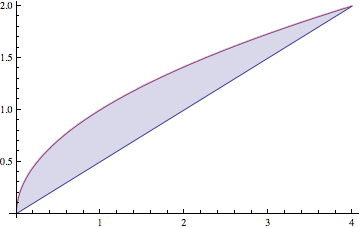
\includegraphics[width=0.4\textwidth]{imgs/AreaInt1.png}
\caption{Integral $I_1$}
\label{imgInt1}
\end{center}
\end{wrapfigure}

Por ejemplo, si tenemos la siguiente integral (ver figura \ref{imgInt1}) \[ I_1 = \int_0^2\int_{y^2}^{2y} f(x,y)\,dx\,dy \] y queremos invertirla cambiamos los límites de integración: \[ I_1 = \int_0^4 \int_{\frac{x}{2}}^{\sqrt{x}} f(x,y)\, dy\,dx \]

Otro ejemplo: estudiemos \[ I_2 = \int_a^bf(x)\,dx = \int_a^b\int_0^{f(x)}dx\,dy \]. Si probamos a cambiar el orden de integración, tenemos que

\[ I_2 = \int_0^M\int_{A(y)}dx\,dy \]

Donde $M$ es el máximo de $f$ y $A(y) = \{ x\in [a,b] \tq f(x) ≥ y \}$. La longitud de ese conjunto $A$ se denomina la medida, y entonces podemos expresar

\[ I_2 = \int_0^\infty \abs{\{x \tq f(x) > y\}}\,dy \] ya que la medida del conjunto será $0$ cuando $y > M$.

Curiosamente, hemos pasado de una integral de Riemann a otra con una expresión distinta, la llamada \textbf{integral de Lebesgue}\index{Integral! de Lebesgue}. Esto pertence al campo de la \textbf{teoría de la medida}, y permite estudiar conjuntos extraños y más monstruos y engendros varios. \label{IntLebesgue}

En general, podemos expresar nuestro cambio de variable de forma más general para cualquier cambio de variable:

\begin{theorem}[Cambio\IS de variable (dimensiones superiores)]
Dados unos conjuntos $D,\,D^\ast$ con $\appl{\Phi}{D}{D^\ast}$ un difeomorfismo, y $\gx \in D;\; \gy \in D^\ast$. Entonces

\[ \int_{D^\ast} f(\gy)\,d\gy = \int_D f(\Phi(\gx)) \abs{\det \dpa{\gy}{\gx}}\,d\gx \]
\end{theorem}

\subsubsection{Integración en curvas}

\begin{defn}[Curva\IS $C^1$]  Se denomina curva en $\real^n$ a una aplicación \begin{align*}
\appl{\gamma}{[a,b]\subset \real&}{\real^n} \\
t&\to \gamma(t) = (x_1(t),\dotsc,x_n(t))
\end{align*}

y con $\gamma\in C^1$.

También exigiremos que la curva sea un \textbf{camino regular}\index{Camino!regular}, es decir que

\[ \gamma'(t) \neq \gor{0} \;\forall t \]

de tal forma que obligamos a que tenga tangente en todo punto.
\end{defn}

Para calcular la longitud aplicamos las ideas básicas del cálculo integral: \textit{troceamos} el intervalo $[a,b]$, y aproximamos cada uno de esos trozos por un segmento. Calculamos la suma de la longitud de esos segmentos, hacemos tender la anchura de los \textit{trozos} y si converge, la longitud se puede medir.

\begin{theorem}[Longitud\IS de una curva] Dada una partición $\mathcal{P} = \{ a= t_0 < t_1 < \dotsb < t_k = b\}$ definimos \[ \abs{\mathcal{P}} = \max_i \abs{t_{i+1} - t_i} \] y la longitud $L$ de la curva.

\[ L(\sigma) = \lim_{\abs{\mathcal{P}}\to 0} \underbrace{\sum_{i=0}^{k-1} \md{\sigma(t_{i+1}) - \sigma(t_i)}}_{=S(\sigma,\mathcal{P})} \]

SI $\sigma\in C^1$, entonces $L(\sigma)$ existe y además

\[ L(\sigma) = \int_a^b \md{\sigma'(t)}\,dt \]

\end{theorem}

Este teorema responde a una idea con respecto al cambio de variable: si tomamos $\Gamma$ como la curva que queremos integrar, entonces se puede expresar

\[ L(\sigma) = \int_\Gamma 1\,d\sigma = \int_a^b \md{\sigma'(t)}\,dt  \]

donde $\md{\sigma'(t)}$ es el cambio en la medida correspondiente.

\begin{proof} Por pura pereza y no escribir más \footnote{A mí también me parece bien} suponemos \[ \sigma(t) = (x(t),y(t)) \]. Tenemos que

\begin{gather*}
 S(\sigma,\mathcal{P}) = \sum_{i=0}^{k-1} \md{\sigma(t_{i+1}) - \sigma(t_i)} = \\
 = \sum_{i=0}^{k-1}\sqrt{\left(x(t_{i+1}-x(t_i)\right)^2 + \left(y(t_{i+1}-y(t_i)\right)^2}
 \end{gather*}

 Por el Teorema del valor medio (\ref{thmTVM1var}) tenemos que

 \begin{gather*}
 \left(x(t_{i+1}-x(t_i)\right)^2  = x'(s_i^1)^2(t_{i+1}-t_i)^2 \\
 \left(y(t_{i+1}-y(t_i)\right)^2  = y'(s_i^2)^2(t_{i+1}-t_i)^2
 \end{gather*}

 Entonces

 \[  S(\sigma,\mathcal{P})  = \sum_{i=0}^{k-1}  (t_{i+1}-t_i) \sqrt{x'(s_i^1)^2 + y'(s_i^2)^2} \]

 No podemos simplificar porque no es seguro que $s_i^1 = s_i^2$. Si fueran el mismo punto, serían sumas de Riemann y habríamos terminado.

 Como tenemos una función continua ($\sigma'$) y estamos trabajando en un intervalo cerrado y acotado ($[a,b]$) podremos reducir la expresión a $\sqrt{x'(t_i)^2 + y'(t_i)^2}$ y que gracias a la continuidad uniforme la diferencia con $\sqrt{x'(s_i^1)^2 + y'(s_i^2)^2}$ se puede hacer todo lo pequeña que queramos, llegando a hacer coincidir en el límite $s_i = t_i$, por lo que podríamos escribir:

\[  S(\sigma,\mathcal{P})  = \sum_{i=0}^{k-1} \sqrt{x'(t_i)^2 + y'(t_i)^2} (t_{i+1}-t_i) \]
  o también:
\[  S(\sigma,\mathcal{P})  = \sum_{i=0}^{k-1} \sqrt{x'(t_{i+1})^2 + y'(t_{i+1})^2} (t_{i+1}-t_i) \]


La forma matemática de escribir este argumento:

Notación: $G(s,t) = \sqrt{(x'(s))^2 + (y'(s))^2}$

Llamamos:
\[(1) = \sum G(s_i^1,s_i^2)(t_{i+1}-t_i)\]
\[(1) = \sum G(t_i^1,t_i^2)(t_{i+1}-t_i)\]

Vamos a estudiar $\abs{(1)-(2)}$

\[0\leq \abs{(1)-(2)} \leq ... \leq \sum_i \abs{G(s_i^1,s_i^2)- G(t_i^1,t_i^2)}(t_{i+1}-t_i)\]

$(s_1^1, s_1^2 \in [t_i,t_{i+1}]$ por tanto:
\[\md{s_i^1,s_i^2) - (t_i,t_i)} = ... \leq \sqrt{2}\md{\mathcal{P}}\]

Aplicamos $G$ continua en $[a,b]\times [a,b]$ (compacto) $\implies G$ uniformemente continua.

\end{proof}

\obs \textbf{Falso} en general si la curva es sólo continua

\paragraph{Ejemplo:}

\[\appl{\sigma}{[0,1]}{\real^2}\]

\todo{A dibujar!}

Descripción gráfica: entre $\frac{1}{2^k}$ y $\frac{1}{2^{k+1}}$ y formo un triángulo isósceles con esos 2 puntos y de altura hasta la bisectriz.

Sea el triangulo K:

\todo{Dibujo}

\[Longitud =L_k = ... ??? ... = \frac{1}{2k+1} \{\sqrt{\frac{1}{4k^2}+1} + \sqrt{\frac{1}{4k^2+4} +1} \} \ge \frac{1}{2k+1}\]
\[\text{Longitud total } = \sum L_k \ge \sum_k \frac{1}{2k+1} = \infty\]

Este mostruito no tiene longitud. ¿Y si en vez de rectas tomamos sinusoides? Esa función si debería ser $C^1$ pero la longitud es $\infty$. Entonces la curva no puede ser $C^1$ (sería un contrajemplo del teorema)

\begin{defn}[Curva\IS rectificable]\label{defCurvaRectf}
Si el límite \[ \lim_{\abs{\mathcal{P}}\rightarrow 0} S(\sigma,\mathcal{P})\] existe entonces $\sigma$ es \textbf{rectificable}.

Además, con comprobar que la curva es $C^1$ es suficiente.

Para que $\sigma$ sea rectificable, basta con que sea continua de Lipschitz, es decir que \[\lim_{x\to x_0} \frac{d(f(x),f(x_0)}{d(x,x_0)}\leq C,\forall x\]

\end{defn}


\subsubsection{Parametrización por longitud de arco}

\[ \appl{\sigma}{[a,b]}{\real^n} \]

con $\sigma$ curva $C^1$ y regular. Entonces

\[ L(s) = \int_a^s \md{\sigma'(t)}\,dt \]

y por el Teorema Fundamental del Cálculo

\[ L'(s) = \md{\sigma'(s)} \]

Al imponer que la curva sea regular, entonces $\sigma'(s)\neq 0$ y por lo tanto existe la inversa $\inv{L}$. Si tenemos entonces un $\tau ∈ [0,L(b)]$, entonces $S=\inv{L}(\tau) ∈ [a,b]$.\wtf

Definimos

\begin{gather*}
\sigma^\ast = \sigma \circ \inv{L} \\
\sigma^\ast = \sigma(\inv{L}(\tau)) \\
(\sigma^\ast)'(\tau) = \sigma'(\inv{L}(tau)) (\inv{L}(\tau))' = \sigma'(\inv{L}(\tau)) \frac{1}{L'(\inv{L}(\tau))} = \sigma'(s) \frac{1}{L'(s)} = \frac{\sigma'(s)}{\md{\sigma'(s)}}
\end{gather*}

Es decir, hemos conseguido una parametrización con velocidad constante $\md{(\sigma^\ast)'} = 1$ y por lo tanto

\[ L(\tau) = \int_0^\tau \md{(\sigma^\ast)'}\,ds = \int_0^s 1\,ds = s \]

\section{Integración en dimensiones superiores}

\subsection{Elemento de área}

Supongamos que estamos en $\real^3$. Podemos hablar de la longitud de una variedad de dimensión 1, del área de una de dimensión 2 o del volumen de una de dimensión 3. Ahora bien, ¿qué ocurre cuando pasamos a dimensiones superiores? La denominación será la siguiente

\begin{itemize}
\item \textbf{1-variedad} Longitud
\item \textbf{k-variedad} $1<k<N$ Área
\item \textbf{N-variedad} Volumen
\end{itemize}

Para calcular esas \textit{cosas} empezaremos partiendo del área de un parelelepípedo.

Definiremos el paralelepípedo como, dados $k$ vectores independientes $\{\gv_i\} \subset \real^N$,

\[ P_k = \sum_{i=1}^k \lambda_i\gv_i\;\lambda_i \in [0,1] \]


Elemento de área: $P_k \equiv \{ \sum_{i=1}^k \lambda_i\gor{v}_i, \lambda_i \in [0,1]\}\subset \real^N$

Definimos una \begin{gather*}
\appl{\Psi}{\real^N}{\real^N}\\
\gx \longrightarrow (\Psi_1(\gx),...,\Psi_n(\gx))
\end{gather*}

\begin{itemize}
\item si $\gx \in P_k \implies \Psi(\gx) = (\Psi_1(\gx),\Psi_2(\gx),...,\Psi_k(\gx),0,...,0)$
\item $\Psi$ mantiene longitudes y ángulos, es decir $\pesc{\Psi(u),\Psi(v)}=\pesc{u,v}, \forall u,v\in\real^N$

Esto implica: $\pesc{\Psi(u),\Psi(v)}=\pesc{u,v} \implies \md{\Psi(\gu)} = \md{\gu}$. Si se conservan los módulos, se conservan también los ángulos.
\end{itemize}

\obs Si $\gx,\gy\in P_k \implies \pesc{\gx,\gy} = \underbrace{\pesc{\Psi(\gx),\Psi(\gy)}}_{\text{Prod } \real^N} = \underbrace{{\tilde{\Psi}(\gx),\tilde{\Psi}(\gy)}}_{\text{Prod } \real^K}$


\textbf{Idea:} Área $(P_k)$ = Área $(\tilde{\Psi}(P_k)) \equiv \displaystyle \int_{\tilde{\Psi}(P_k)}d\gor{s}$, una integral en $\real^K, K<N$



El paso que vamos a dar ahora es: Construir una aplicación $L$ tal que $L(\gor{e}_i) = \tilde{\Psi}(\gor{v}_i)$

Y aplicamos el cambio de variables:
\[\int_{\tlps(P_k)} d\gor{s} = \int_{[0,1]^K} \abs{\det\left( \dpa{s}{t} \right)} d\gor{t}\]

Tenemos:
\begin{itemize}
\item $L$ lineal, $\appl{L}{\real^K}{\real^K}$
\item $L(\gor{e}_j) = \tlps(\gv_j)$.
\end{itemize}
Con la segunda propiedad podemos construir la aplicación $L$.

\begin{gather*}
L = \begin{pmatrix} \tlps(\gv_1) & \tlps(\gv_2) & ... & \tlps(\gv_k)\\
\downarrow & \downarrow & \ddots & \downarrow
\end{pmatrix} = \frac{d\gor{s}}{d\gor{t}}\end{gather*}

\textbf{Conclusión:} \[Area(P_k) = \abs{\det L} = \left|\det \begin{pmatrix}
\tlps(\gv_1) & \tlps(\gv_2) & ... & \tlps(\gv_k)\\
\downarrow & \downarrow & \ddots & \downarrow
\end{pmatrix}\right|\]

Pero... tenemos 2 problemas:
\begin{itemize}
\item Necesitamos una manera cómoda con la que construir $\tlps$.
\item ¿Utilizando otra parametrización llegamos al mismo resultado?
\end{itemize}

Vamos a reventar 2 pajaros de un tiro.

\[ Area(P_k) = \left( \det \begin{pmatrix}
\tlps(\gv_1) & \tlps(\gv_2) & ... & \tlps(\gv_k)\\
\downarrow & \downarrow & \ddots & \downarrow
\end{pmatrix}
\begin{pmatrix}
\tlps(\gv_1) & \tlps(\gv_2) & ... & \tlps(\gv_k)\\
\downarrow & \downarrow & \ddots & \downarrow
\end{pmatrix} ^T \right)^{\frac{1}{2}}\]
¿Qué ganamos?
\[\begin{pmatrix}
\pesc{\tlps(\gv_1),\tlps(\gv_1)} & \pesc{\tlps(\gv_1),\tlps(\gv_2)} & ... & \pesc{\tlps(\gv_1),\tlps(\gv_k)}\\
\pesc{\tlps(\gv_2),\tlps(\gv_1)} & \pesc{\tlps(\gv_2),\tlps(\gv_2)} & ... & \pesc{\tlps(\gv_2),\tlps(\gv_k)}\\
\vdots & \vdots & \ddots & \vdots\\
\pesc{\tlps(\gv_k),\tlps(\gv_1)} & \pesc{\tlps(\gv_k),\tlps(\gv_2)} & ... & \pesc{\tlps(\gv_k),\tlps(\gv_k)}
\end{pmatrix} = (\ast) = \left(\det(\pesc{v_i,v_j})\right)^{\frac{1}{2}}\]
($\ast$) Hemos construido las cosas de tal manera que se mantiene el producto escalar.

\paragraph{Ejemplo: } $P_2 \subset \real^3$ generado por $\gu,\gv\in\real^2$

$Area(P_2) = \left(\det \begin{pmatrix}
\pesc{\gu,\gu} & \pesc{\gu,\gv}\\
\pesc{\gv,\gu} & \pesc{\gv,\gv}
\end{pmatrix} \right)^{\frac{1}{2}} = \left(\pesc{\gu,\gu}\pesc{\gv,\gv} - \pesc{\gu,\gv}^2\right)^{\frac{1}{2}} =\left(\md{\gu}\md{\gv} - \md{\gu}\md{\gv}(cos(\theta)^2)\right)^2 = \md{u}\md{v} \sqrt{1-cos^2(\theta)}  =  \md{u}\md{v} sen(\theta) = ||u\times v||$

Bueno, esto cumple lo que la sabíamos de selectividad. El área de un paralelogramo 2 dimensional en $\real^3$ es la raiz cuadrada del módulo del producto vectorial.

\textbf{Aplicación:} Vamos a aplicar esto para hallar el área de una $k-variedad$ en $\real^N$.

\todo{Dibujo}
\begin{itemize}
\item $\Phi(\gs_0) = \gx_0 \in M$
\item $\Phi(\gs_0 + h_j\gor{e}_j) = \Phi(\gs_0) + \dpa{\Phi}{s_j}(\gs_0)\cdot h_j + err(h)$
Aplicando taylor, en el que cada alargamiento $h$ depende de la dirección.
\end{itemize}

\textbf{Idea:} $Area(\Phi(Q_k)) = Area(P_k) + err(h)$ donde $Area(P_k) = \left(\det (\pesc{v_i,v_j})\right)^{\frac{1}{2}}, \{v_j\}$ genera $P_k$.

\todo{Me he perdido porque $v_i = \dpa{\Phi}{s_j}(\gs_0)\cdot h_j$}

\[\left(\det\left(\pesc{\dpa{\Phi}{s_i},\dpa{\Phi}{s_j}}h_ih_j\right)\right)^{\frac{1}{2}}\]

Tomamos $h_i = h, \forall i$

\[\underbrace{\underbrace{h^k}_{Area(Q_k)} \left(\det\left(\pesc{\dpa{\Phi}{s_i},\dpa{\Phi}{s_j}}\right)\right)^{\frac{1}{2}}}_{Area(P_k)}\]

Conclusión: \[Area(M) = \sum_n Area(Q_k^n) \left(\det\left(\pesc{\dpa{\Phi}{s_i}(\gs_0^n),\dpa{\Phi}{s_j}(\gs_0^n)}\right)\right)^{\frac{1}{2}} + err(h)\]

Si llamamos $F(s_0^n) = \left(\det\left(\pesc{\dpa{\Phi}{s_i}(\gs_0^n),\dpa{\Phi}{s_j}(\gs_0^n)}\right)\right)^{\frac{1}{2}}$

Tenemos: \[\sum_n Area(Q_k) F(s_0^n) \convs[Riemann] \int_D F(\gs)d\gs\]

\textbf{Por tanto:} $Area(M) = \int_D \left(\det\left(\pesc{\dpa{\Phi}{s_i},\dpa{\Phi}{s_j}}\right)\right)^{\frac{1}{2}}$

Lo que en Cálculo 2 llamábamos $\md{T_u\times T_v}$.


Dada una $\appl{f}{\real^N}{\real}$ podemos definir: \[\int_{\Phi(D)}f dA = \int_{D}f(\Phi(s)) \left(\det(\pesc{\Phi_{s_i},\Phi_{s_j}})\right)^{\frac{1}{2}} ds\]

\paragraph{Ejemplos}

\subparagraph{Ejemplo 1)}

\[\appl{\sigma}{[a,b]}{\real^N}\]

Sea $\Gamma = \{\sigma(t)\in\real^N\tq t\in[a,b]\}$

El elemento de área sería:

\[\int_{\Gamma} fdA = \int_a^bf(\sigma(t)) (\pesc{\sigma',\sigma'})^{\frac{1}{2}}\]


\subparagraph{Ejemplo 2)}

\[
\Phi : D\subset\real^2\rightarrow \real^3\]
\[(s_1,s_2)\rightarrow (x(s_1,s_2),y(s_1,s_2),z(s_1,s_2))\]

Tenemos en este caso:
\[\int_{\Phi(D)}fdA = \int_D f(\Phi(s_1,s_2)) (\det(\pesc{\Phi_{s_i},\Phi_{s_j}}))^{\frac{1}{2}})ds\]
\[(\det(\pesc{\Phi_{s_i},\Phi_{s_j}}))^{\frac{1}{2}}) = (*) = \md{\Phi_1 \times \Phi_2}\]
$(*)$ visto anteriormente.

Integrales de \textbf{campos} sobre \textbf{curvas} y \textbf{superficies} en $\real^3$.

\begin{itemize}
\item[1] $\Gamma$ curva, $\overrightarrow{F}$ campo. Nos interesa la componente que sigue la tangente de la recta (ya que en la dirección perpendicular no se realiza trabajo). Para ello multiplicamos escalarmente por el vector director normalizado.
\[\int_{\Gamma} \overrightarrow{F}d\sigma \equiv \text{ Trabajo } \equiv \int_{\Gamma} F_T = \int_{\Gamma} \pesc{\overrightarrow{F},\frac{\sigma'}{\md{\sigma'}}}\]
\[ = \int_a^b \pesc{\overrightarrow{F}(\sigma(t)),\frac{\sigma'(t)}{\md{\sigma'(t)}}} \md{\sigma'(t)}dt = \int_a^b \pesc{\overrightarrow{F}(\sigma(t)),\sigma'(t)} dt\]

\item[2] Flujo a través de una superficie.

En este caso, la componente que nos interesa es la perpendicular a la superficie.

$\overrightarrow{n} = T_u\times T_v$

\[\int_{\Phi(D)} \overrightarrow{F} = ... = \int_{D} \pesc{\overrightarrow{F}(\Phi(u,v)),T_u\times T_v}dudv\]
\end{itemize}

Volvemos a plantearnos el problema: ¿Distintas parametrizaciones nos da el mismo trabajo/flujo? Depende de la \textit{orientación} de la parametrización. No es lo mismo el trabajo para ir desde abajo de la curva hasta arriba que para bajarla. ¿Este problema traducido a $\real^K$, flipas o k ase?


Recordamos algunos teoremas y definiciones vistos en Calculo 2:

\subsection{Campos vectoriales}
Los campos vectoriales son funciones $\appl{F}{\real^N}{\real^N}$, en el que a cada punto se le asigna un vector.
\index{Campo!vectorial}

\begin{defn}[Campo\IS conservativo]
Diremos que $F$ es un campo gradiente o conservativo si $\exists \appl{V}{\real^N}{\real}$ tal que $F=\nabla V$.
\end{defn}

\begin{defn}[Divergencia]
En un campo vectorial, la divergencia mide el cambio de volumen y existencia de fuentes o sumideros. Si la divergencia es 0, tenemos un "fluido" incompresible.

\[ \textrm{div}\;F = \frac{∂F_1}{∂x_1} + \cdots + \frac{∂F_n}{∂x_n} \]
\end{defn}

\begin{defn}[Rotacional]
El rotacional mide el giro interno de las partículas en un campo, que se puede expresar como \footnote{En realidad, $\nabla$ no es un vector y esto es sólo una regla mnemotécnica}

\[ \textrm{rot}\;F = \nabla \x \vf \]

Si el rotacional es distinto de cero, significa que ha habido choques internos de las partículas y por lo tanto ha habido pérdida de energía.
\end{defn}

\begin{theorem}
Supongamos que $F\in C^1$ es un campo gradiente. Entonces, $\rot F = \vec{0}$. El recíproco también es cierto.
\end{theorem}


\begin{theorem}[Teorema\IS de Green]
Sea $\Gamma$ una curva simple en $\real^2$. Llamamos $D$ al interior de $\Gamma$. Sea $(P,Q)$ el campo con $P,Q\in C^1(D)$. Entonces

\[ \int_{\Gamma^+} (P,Q)\dif \sigma = \iint_D \frac{\partial Q}{\partial x}-\frac{\partial P}{\partial y}\id{x,y} \]
\end{theorem}

\begin{theorem}[Teorema\IS de Stokes]
Dada $\Gamma$ una curva cerrada simple en $\real^3$ que es el borde de una superficie $S$, tenemos que

\[ \int_{\Gamma^+}\vec{F}\dif \sigma =\iint_{S^+}\rot \vec{F}\dif S \]

Esto indica que el flujo por una superficie depende sólo de la forma de su boca.
\end{theorem}

\begin{theorem}[Teorema\IS de Gauss]
Sea $S$ una superficie cerrada que encierra una región $\Omega$, y $\vec{F}\in C^1(\Omega)$.

\[ \iint_{S^+} \vf \dif S = \iiint_\Omega \dv \vec{F}\, \id{x,y,z} \]
\end{theorem}


Todos estos teoremas son parecidos en cuanto a que a la izquierda se tiene el campo evaluado en la frontera y a la derecha tenemos una integral en el interior de una expresión más o menos compleja en la que aparecen las derivadas. Cabe esperar que sean casos particulares de un teorema superior, cosa que es cierta. Este teorema se le llama de \textbf{Stokes} en general.

De aquí al final de curso nos dedicaremos a llegar a ese teorema y ver que estos 3 teoremas son casos particulares.

Para ello nos adentraremos en el espinoso jardín de la orientación.

\subsection{Orientación}
El tema de la orientación tiene que ver con tener cuidado con el orden. Vamos a ver los ejemplos de pocas dimensiones:

\paragraph{Ejemplos:}

\subparagraph{Ejemplo 1) Bases en $\real^2$}

\[\mathcal{B}_1 = \{(0,1),(1,0)\}\]
\[\mathcal{B}_2 = \{(1,0),(0,1)\}\]

Sea $\gv = (v_1,v_2)_{\mathcal{B}_1} = (v_2,v_1)_{\mathcal{B}_2} \neq \gv$

Lo que haremos en este caso será un cambio de base, $\mathcal{B}_1,\mathcal{B}_2$ bases en $\real^N$. Sea $\mathcal{C}_{\mathcal{B}_1\to\mathcal{B}_2}$ matriz del cambio de base de $\mathcal{B}_1$ a $\mathcal{B}_2$.

\begin{defn}[Orientación]
Diremos que $\mathcal{B}_1,\mathcal{B}_2$ tiene la misma orientación $\dimplies \det \mathcal{C}_{\mathcal{B}_1\to\mathcal{B}_2} > 0$
\end{defn}

¿Que pasaría si el determinante de esa matriz de cambio de base sea 0? No puede ser (por definición de cambio de base, que tiene que ser reversible).

\subparagraph{Ejemplo 2)} $\real^3$.
Sean
\[\mathcal{B}_1 = (\gu,\gv,\gw),\mathcal{B}_2 = (\gv,\gu,\gw),\mathcal{B}_3 = (\gw,\gu,\gv)\]

Si tomamos $\gu = \begin{pmatrix} 1\\0\\0\end{pmatrix}_{\mathcal{B}_1} = \begin{pmatrix}0\\1\\0\end{pmatrix}_{\mathcal{B}_2} = \begin{pmatrix}0\\1\\0\end{pmatrix}_{\mathcal{B}_3} $

Siguiendo este razonamiento llegamos a la matriz de cambio de base:

\[\mathcal{C}_{\mathcal{B}_1\to\mathcal{B}_2} = \begin{pmatrix} 0 & 1 & 0 \\ 1 & 0 & 0 \\ 0 & 0 & 1 \end{pmatrix}\]
Cuyo determinante es negativo.

Lo mismo con

\[\mathcal{C}_{\mathcal{B}_1\to\mathcal{B}_1} = \begin{pmatrix} 0 & 0 & 1 \\ 1 & 0 & 0 \\ 0 & 1 & 0 \end{pmatrix}\]
Cuyo determinante es positivo.

¿Porqué al cambiar el orden se cambia la orientación?

\obs Aceptamos como orientación positiva la de la base canónica ordenada como Dios manda: $\{(1,0,0,...,0), (0,1,0,0,...,0), (0,0,1,0,0,...,0),...,(0,0,...,0,1)\}$

Vamos con algún ejemplo más:

\subparagraph{Ejemplo 3)} (Importante)

En $\real^3$, sean $\gu,\gv$ independientes.

Construimos $\mathcal{B} = \{\gu,\gv,\gu\times\gv\}$. Queremos saber si esta base es de orientación positiva u orientación negativa.

\[\gu\times\gv = \left|
\begin{array}{ccc}
 \overrightarrow{i} & \overrightarrow{j} & \overrightarrow{k}\\
u_1 & u_2 & u_3 \\
v_1 & v_2 & v_3
 \end{array}\right| = ... = \left(\left|\begin{array}{cc}u_2&v_2\\u_3&v_3\end{array}\right|,\left|\begin{array}{cc}u_1&v_1\\u_3&v_3\end{array}\right|,-\left|\begin{array}{cc}u_1&v_1\\u_2&v_2\end{array}\right|\right)\]

 \[\mathcal{B}_{\mathcal{B}\to\mathcal{C}} = \begin{pmatrix}
u_1&v_1& \left|\begin{array}{cc} u_2&v_2\\u_3&v_3 \end{array}\right|\\

u_2&v_2& -\left|\begin{array}{cc} u_1&v_1\\u_3&v_3 \end{array}\right|\\

u_3&v_3& \left|\begin{array}{cc} u_1&v_1\\u_2&v_2\end{array}\right|
 \end{pmatrix}\]

 Cuyo determinante es \[\left|\begin{array}{cc}u_2&v_2\\u_3&v_3\end{array}\right|^2+\left|\begin{array}{cc}u_1&v_1\\u_3&v_3\end{array}\right|^2+\left|\begin{array}{cc}u_1&v_1\\u_2&v_2\end{array}\right|^2>0\]


\subparagraph{Ejemplo 4)} $\real^2$

Sean \[\mathcal{C} = \{(1,0),(0,1)\}\]
\[\mathcal{B} = \{(u_1,u_2),(v_1,v_2)\}\]

La matriz fácil de calcular es \[C_{\mathcal{B}\to \mathcal{C}} = \begin{pmatrix} u_1&v_1\\u_2&v_2\end{pmatrix}\]
\[0<\det \begin{pmatrix} u_1&v_1\\u_2&v_2\end{pmatrix}  = \pesc{(u_1,u_2),(v_1,v_2)} = \pesc{(\lambda,0),(\beta,-\alpha)} = \lambda\beta\]

Aplicando un giro (de aquí salen $\lambda$...) podemos ver que el si el ángulo entre $\gu,\gv \in (0,\pi) \leadsto +$ pero si el ángulo entre $\gu,\gv \in (\pi,2\pi) \leadsto -$. ¿Y en $\pi$? Entonces los vectores no serían independientes.

\textbf{Idea:} Vamos a dedicarnos a jugar con los vectores de la base aplicandoles una deformación continua para ver que pasa con la discontinuidad de la orientación en $\pi$ a ver que encontramos.

Sea la deformación $(\alpha(t),\beta(t)), t\in(0,1)$ continua, donde $(\alpha(0),\beta(0)) = (e_1,e_2)$ y $(\alpha(1),\beta(1)) = (e_1,e_2)$

\begin{itemize}
\item
Si la orientación de la base que tengo al final es positiva, entonces podemos encontrar una transformación continua que mantenga positivo el determinante, $\forall t$.
\item
Si la orientación es negativa, entonces \textbf{siempre} det=0 para algún $t$.
\end{itemize}

\paragraph{Vamos a extender la idea anterior} en $\real^3$.

Idea geométrica: Yo tengo 2 bases y quiero pasar de una a otra, si puedo encontrar un camino en el que los 3 vectores nunca pertenezcan al mismo plano entonces la orientación es la misma. \textbf{El orden es fundamental}.

Sea
\[\mathcal{B} = \{e_1,e_2,e_3\} \hspace*{150pt} \mathcal{C} = \{\gu,\gv,\gw\}\]


\hspace*{50pt}
\begin{tikzpicture}[baseline=(X.base)]
\def\R{2.5} % sphere radius
\def\angEl{15} % elevation angle
\def\angAz{-105} % azimuth angle
\def\angPhi{-40} % longitude of point P
\def\angBeta{19} % latitude of point P


%Ecuador
\pgfmathsetmacro\H{\R*cos(\angEl)} % distance to north pole

\tikzset{xyplane/.estyle={cm={cos(\angAz),sin(\angAz)*sin(\angEl),-sin(\angAz),
                              cos(\angAz)*sin(\angEl),(0,0)}}}
\draw[xyplane,<->] (3,0) node[below] {$e_1$} -- (0,0) -- (0,3)
    node[right] {$e_2$};
\draw[->] (0,0) -- (0,3) node[above] {$e_3$};

\end{tikzpicture}
\hspace*{100pt}
\begin{tikzpicture}[baseline=(X.base)]

\def\R{2.5} % sphere radius
\def\angEl{15} % elevation angle
\def\angAz{-105} % azimuth angle

\tikzset{xyplane/.estyle={cm={cos(\angAz),sin(\angAz)*sin(\angEl),-sin(\angAz),
                              cos(\angAz)*sin(\angEl),(0,0)}}}
 \draw[xyplane,<->] (3,0) node[below] {$\gu$} -- (0,0) -- (0,3)
    node[right] {$\gv$};
\draw[->] (0,0) -- (0,-3) node[right] {$\gw$};
\end{tikzpicture}

No hay ninguna manera de llevar $e_3$ a $\gw$ sin formar un único plano con los tres vectores.

Aunque podríamos llevar $e_3 \to \gu$ y $e_1 \to \gw$... ¿Entonces?

Mal! Porque no estamos manteniendo el orden, tendríamos la base $\mathcal{C}* = \{\gw,\gv,\gu\}\neq\mathcal{C}$.


\paragraph{Caracterización práctica}
\begin{lemma}
\label{thmProdVect} Si $\gu,\gv$ son vectores independientes, entonces $\{ \gu,\gv,\gu\times\gv \}$ es una base.
\end{lemma}

\begin{lemma} La base $\{\gu,\gv,\gw\}$ tiene orientación positiva si y sólo si $\gw$ y $\gu\times\gv$ están en el mismo lado del espacio respecto del plano generado por $\gu,\gv$ (o, lo que es lo mismo, $\pesc{\gw,\gu\x\gv} > 0$).
\end{lemma}

Ahora que ya tenemos vista la orientación de bases en $\real^N$ vamos a ver la orientación en $T_a M$ (espacio tangente de una variedad en un punto)

\todo{Tipico dibujo de un conjunto en el plano $\real^K$ que la parametrización $\Phi$ lo lleva al espacio.}

Sea $\{e_1,e_2,\dotsc,e_k\}$ la base canónica en $\real^k$, y $\Phi(u_0)=\ga$

Como la variedad viene dada por una parametrización, tomamos $\img D\Phi$, es decir: \[T_{\ga}M = \img D\Phi(u_0)  = \{D\Phi(u_0)\gv,\gv\in\real^K\}\]
Tomando la base euclídea:
\[D\Phi(u_0) \{\sum^k v_i\gor{e}_i\}\equiv \sum^k v_i\underbrace{[D\Phi(u_0)\gor{e}_i]}{\in\real^N} \]

\subparagraph{1)}Es decir, la $\img D\Phi$ está generada por los k vectores \begin{equation}\label{baseTaM}
\{ D\Phi(u_0)\gor{e}_1,\dotsc ,D\Phi(u_0)\gor{e}_k \}
\end{equation}

\subparagraph{2)}
La condición de rango máximo nos asegura que los $k$ vectores son linealmente independientes.

\paragraph{Conclusión:} El conjunto (\ref{baseTaM}) es una base de $T_{\ga}M$

\textit{Problema} Si tenemos 2 parametrizaciones distintas $\Phi,\Psi$ entonces tendremos 2 bases diferentes. Cabe plantearse bajo qué condiciones se mantiene la orientación. (aunque todavía no tengamos muy claro que es la orientación de una variedad)

\paragraph{Ejemplos:}
\subparagraph{1)} Las orientaciones de una curva en $\real^N$ es fácil, basta comprobar los sentidos de los vectores tangentes.

Vamos a hacer las cuentas:

Sean $\sigma,\beta$ parametrizacones del mismo trozo de la curva, que parten de orígenes distintos.

\[\appl{\sigma}{U}{\Gamma},s\to \sigma(s)\]
\[\appl{\beta}{V}{\Gamma},t\to \beta(t)\]

Tenemos un teorema que nos garantiza que existe un \textbf{difeomorfismo} (\ref{TeoremaDifeomorfismo})g, tal que \[\sigma(s) = \beta(g(s)) \y \sigma'(s) = \beta'(g(s))\cdot g'(s)\]

En este caso, para que las dos parametrizaciones den la misma orientación, $g'>0$.

\subparagraph{2)} Las orientaciones de una superficie también, basta comprobar los sentidos de los vectores normales.

\[\appl{\Phi}{U}{\real^3}, (u,v) \to \Phi(u,v)\]
\[\appl{\Psi}{V}{\real^3}, (r,s) \to \Psi(r,s)\]

Tenemos un teorema que nos garantiza... tal que \[g(u,v) = (g_1(u,v),g_2(u,v))\]

En este caso, calculamos \[\left.\begin{array}{c}
\Phi_u\times\Phi_v \\
\Psi_r\times\Psi_s
\end{array}\right\}\]

Tenemos que $\Phi(u,v) = \Psi(g_1(u,v),g_2(u,v))$

\begin{gather*}
\Phi_1(u,v) = \Psi_1(g_1(u,v),g_2(u,v))\\
(\Phi_1)_{u} = (\Psi_1)_r r_u + (\Psi_1)_s s_u = ((\Psi)_r\,(\Psi_1)_s)\begin{pmatrix}
(g_1)_u\\(g_2)_v
\end{pmatrix}
\end{gather*}
Se calculan las 6 derivadas $(\Phi_1,\Phi_2,\Phi_3)$ respecto de $u$ y de $v$ \emph{Teniendo cuidado de en donde evaluamos que derivadas} y acabamos llegando a

\[\begin{pmatrix}
(\Phi_1)_u\\(\Phi_2)_u\\(\Phi_3)_u
\end{pmatrix} = \begin{pmatrix}
(\Psi_1)_r & (\Psi_1)_s\\
(\Psi_2)_r & (\Psi_2)_s\\
(\Psi_3)_r & (\Psi_3)_s
\end{pmatrix}\begin{pmatrix}
(g_1)_u\\
(g_2)_u
\end{pmatrix}
\]
Análogamente:
\[\begin{pmatrix}
(\Phi_1)_v\\(\Phi_2)_v\\(\Phi_3)_v
\end{pmatrix} = \begin{pmatrix}
(\Psi_1)_r & (\Psi_1)_s\\
(\Psi_2)_r & (\Psi_2)_s\\
(\Psi_3)_r & (\Psi_3)_s
\end{pmatrix}\begin{pmatrix}
(g_1)_v\\
(g_2)_v
\end{pmatrix}
\]

Ahora procedemos a calcular
\[\Phi_u\x\Phi_v = \dotsc = \left(
\left|\begin{array}{cc}
(\Phi_2)_u & (\Phi_2)_v\\
(\Phi_3)_u & (\Phi_3)_v
\end{array}
\right|,-
\left|\begin{array}{cc}
(\Phi_1)_u & (\Phi_1)_v\\
(\Phi_3)_u & (\Phi_3)_v
\end{array}
\right|,
\left|\begin{array}{cc}
(\Phi_1)_u & (\Phi_1)_v\\
(\Phi_2)_u & (\Phi_2)_v
\end{array}
\right|
\right)\]

Tomando el primer elemento calculamos:

\[
\det\left(
\begin{array}{cc}
(\Psi_2)_r & (\Psi_2)_s\\
(\Psi_3)_r & (\Psi_3)_s
\end{array}
\right)\begin{pmatrix}
(g_1)_u &(g_1)_v \\
(g_2)_u & (g_2)_v
\end{pmatrix} =
\left| \begin{array}{cc}
(\Psi_2)_r & (\Psi_2)_s\\
(\Psi_3)_r & (\Psi_3)_s
\end{array}\right| \det Dg
\]

Repitiendo la cuenta con el resto de los elementos, llegamos a

\[\Phi_u\x\Phi_v = \Psi_r\x\Psi_s\cdot (\det Dg)\]

\paragraph{Conclusión} Para mantener la orientación necesitamos $\det Dg > 0$

\begin{defn}[Orientación \IS en $\real^N$]
Sean $\Phi,\Psi$ parametrizaciones de una subvariedad k-dimensional en $\real^N$, con $g \equiv$ cambio de variables tal que $\Phi=\Psi \circ g$.
Entonces $\Phi,\Psi$ inducen la misma orientación $\dimplies \det Dg>0$
\end{defn}

\obs Este teorema solo afecta a la zona de la subvariedad $M$ parametrizada por $\Phi$ y $\Psi$ al mismo tiempo.

\paragraph{Ejemplo de superficies no orientables}

\subparagraph{Banda de Moebius}
\begin{center}
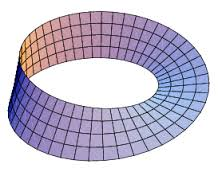
\includegraphics[width=0.5\textwidth]{imgs/Moebius.jpg}
\end{center}
\index{Banda de Moebius}


La parametrización es
\[
\Phi(t,\theta) = \left((R+t\cdot sen\frac{\theta}{2})cos\theta, (R+t\cdot sen\frac{\theta}{2})sen\theta, t cos\frac{\theta}{2} \right) \, t\in(-1,1),\theta\in(0,2\pi)
\]

¿Estamos seguros de que es una parametrización?
\begin{itemize}
\item Regular ($C^1$)
\item $D\Phi$ rango máximo (Fácil)
\item Homeomorfismo
\end{itemize}

Vamos a comprobar el homeomorfismo,

Tenemos 2 posibles caminos:

\subparagraph{1)} Despejamos  en función de $x,y,z$

$\frac{y}{x} = tg \theta$.

Definimos \footnote{Utilizando: (\ref{ImgCirc2})}: \[
\begin{array}{ccc}
\theta &= arctg\frac{y}{x} & (1)\\
\theta &= arctg\frac{y}{x} + \pi & (2)\\
\theta &= arctg\frac{y}{x} + 2\pi & (3)
\end{array}
\]
Y comprobar que es continua


\subparagraph{2)} Escribimos este conjunto como un conjunto de nivel y ver que es una variedad, por lo tanto no hace falta comprobar el homeomorfismo sobre la imagen.

\begin{gather*}
\sqrt{x^2+y^2} = (R + t\cdot cos\frac{\theta}{2})\\
\sqrt{x^2+y^2} - R = \frac{z}{tg\frac{"arctg\frac{y}{x}"}{?}}
\end{gather*}


\subparagraph{Orientación}

Una clave importante es que cuando $\theta\rightarrow 0^+ \implies \Phi(t,\theta)$ pero si $\theta\rightarrow 2\pi^{-} \implies \Phi(-t,\theta)$

$\overrightarrow{n} = T_t\x T_{\theta} = ... = \overrightarrow{n}(t,\theta)$

\begin{gather*}
\overrightarrow{n}(t,\theta) \convs[][\theta\rightarrow 0^+] (-R,\frac{t}{2})\\
\overrightarrow{n}(t,\theta) \convs[][\theta\rightarrow 2\pi^-] (R,-\frac{t}{2})
\end{gather*}

Curioso: esta parametrización que no cubre el segmento con el que se empieza. Esta parametrización tiene una propiedad curiosa, al empezar, el vector normal apunta hacia dentro y al final, apunta hacia fuera. Es imposible cubrirla del todo con una parametrización.

\paragraph{El otro ejemplo} típico de superficie no orientable es la botella de Klein

\begin{center}
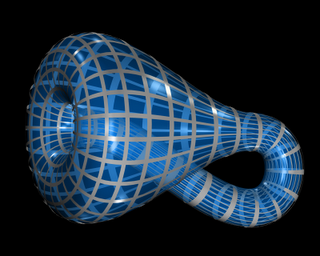
\includegraphics[width=0.5\textwidth]{imgs/botella-de-klein.png}
\end{center}


\paragraph{Variedades con borde}

Conjuntos con frontera en $\real^2$.

Utilizamos la tercera caracterización de subvariedad, que dice que existe un \textbf{difeomorfismo} que vamos a llamar $\Phi$, (que por ser difeomorfismo, existe $\Psi = \Phi^{-1})$.

Podemos suponer que estamos trabajano con un cuadrado en el plano y su imagen para facilitar las cuentas.

Partimos de \begin{itemize}
\item $\Psi(s_0,0) = (x_0,y_0)\in dM$ (la frontera de $M$)
\item $\Psi(s_0,0) \in dM$
\item $\Psi(s,t) \in M, t>0 (s,t)\in U$
\end{itemize}

En U es fácil orientar un cuadrado. ¿Cómo nos "llevamos" la orientación? Con la diferencial, que si queremos que sea la misma orientación $\implies \det D\Phi > 0$.

Sea $\mathcal{C} = \{e_1=(1,0),e_2=(0,1)\}$ base canónica en $\real^2$ (variables (s,t)).

Sea $\mathcal{B} = \{D\Psi(s_0,0)e_1,D\Psi(s_0,0)e_2\}$ base en $\real^2$ (variables $(x,y)$)

Tenemos también $\sigma(s) = \Psi(s,0)$ parametrización de un trozo de $dM$ que contiene a $x_0$.

\[D\Psi = \begin{pmatrix}
\displaystyle\dpa{\Psi_1}{s} &\displaystyle\dpa{\Psi_1}{t}\\
\displaystyle\dpa{\Psi_2}{s} &\displaystyle\dpa{\Psi_2}{t}
\end{pmatrix}\]
En la primera columna lo que tenemos es el vector tangente a la curva. Cuando $t=0$ tenemos la parametrización de la frontera.

\[
D\Psi|_(s_0,0) = \begin{pmatrix}
\sigma'(s_0) & \overrightarrow{v}\\
\downarrow & \downarrow
\end{pmatrix}
\]

Haciendo un desarrollo de Taylor tenemos:

\[
\Psi(s_0,t) = \begin{pmatrix}
\Psi_1(s_0,0)\\
\Psi_2(s_0,0)
\end{pmatrix} + t \underbrace{\begin{pmatrix}
\dpa{\Psi_1}{t} (s_0,0)\\
\dpa{\Psi_2}{t} (s_0,0)
\end{pmatrix}}_{\gor{v}} + err
\]

\[\underbrace{\begin{pmatrix}\Psi_1(s_0,t)\\
\Psi_2(s_0,t)
\end{pmatrix} }_{\in M\, t>0}= \gor{x}_0 + t\gv + err
\]
Conclusión: $\gv$ "apunta hacia el interior de $M$".

\subparagraph{Orientación}
\[\mathcal{C} = \{e_1,e_2\}\]
\[\mathcal{B} = \{D\Psi(s_0,0)e_1,D\Psi(s_0,0)e_2\} = \{\sigma'(s_0),\gv\}\]

\[\mathcal{B} \text{ orientación positiva } \dimplies \det D\Psi(s_0,0) > 0 \dimplies \text{ Ángulo entre } \sigma'(s_0) \text{ y } \gv \in (0,\pi)\]

Con un dibujo se llegaría a entender perfectamente  la siguiente conclusión (basada en la interpretación geométrica de que el ángulo $\in (0,\pi)$)

\index{Orientación\IS de una subvariedad}
\textbf{Conclusión} si recorremos la frontera de la subvariedad	 con la mano izquierda hacia dentro es la orientación positiva si nuestra subvariedad queda en el interior de esa frontera/curva, si nuestra subvariedad es el exterior de la curva pues será la orientación negativa.

\paragraph{Ejemplo}

\[\appl{\Phi}{\real^2}{\real^3}\]

Tenemos $\sigma(s) = \Phi(s,0) $, parametrización de un trozo de $dM$ que contiene a $x_0$.

Siendo \[D\Phi(s_0,0) = \begin{pmatrix}
...
\end{pmatrix} = \begin{pmatrix}
\sigma'(s_0) & \overrightarrow{v}\\
\downarrow & \downarrow
\end{pmatrix}\]

\textbf{Orientación:}

\[\mathcal{C}  = \{e_1,e_2,e_3\}\]

\[\mathcal{B} = \{D\Phi(s_0,0)e_1,D\Phi(s_0,0)e_2\} = \{\sigma'(s_0),\gv\}\]

Pero... solo tenemos 2 vectores, ¿y el tercero? Anteriormente hemos visto que es el producto vectorial (\ref{thmProdVect})

Es decir

\[\mathcal{B} = \{\sigma'(s_0),\gv,\sigma'(s_0)\x\gv\}\]

Con las cuentas vistas antes del ejemplo comprobamos que $\gv$ apunta hacia el interior de $M$.

\textbf{Conclusión:} La elección de $\sigma'$ y del producto vecotiral deben ser compatibles. Para esta elección aplicaríamos la regla del muñequito y la mano izquierda.



\section{Lenguaje de las formas diferenciales}

\paragraph{0-formas}
\index{Formas\IS 0}

Son funciones escalares definidas en un abierto de $\real^n$
\[\appl{f}{\Omega\subset\real^N}{\real}\]

Operaciones habituales:
\begin{itemize}
\item Suma: sí
\item Producto: sí
\item Composiciones: no (porque no cuadran las dimensiones)
\end{itemize}

\paragraph{1-formas}
\index{Formas\IS 1}

Sea $\mathcal{C} = \{e_1,e_2,...,e_n\}$ la base canónica en $\real^N$.

Sea $L$ una aplicación lineal
\[\appl{L}{\real^N}{\real}\]

Que recordamos que cumplen:
\[ L(\gx+\gy) = L(\gx)+L(\gy); L(\lambda\gx) = \lambda L(\gx)\]

Definimos $\gy\in\real^N \leadsto \gy = \displaystyle\sum_1^n y_i e_i$, con lo que \[L(\gy) = \sum y_i L(e_i)\]

Entonces \[\left.\begin{array}{cc}
v_i = L(e_i)\\
y_i = P_i(\gy)
\end{array}\right\} \rightarrow L(\gy) = \sum_i v_iP_i(y)\]

Siendo $P_i$ las proyecciones, una base del espacio dual.

\textbf{Notación:}

$P_i \equiv dx_i$.

$dx_i[\gy] \equiv P_i(\gy) = y_i$

Entonces, dado un $\gv$ podemos construir 
\[L \equiv \sum_i^N v_idx_i\]

\[L[\gy] = \sum_i^N v_idx_i[\gy] = \sum_i^N v_iy_i\]

\begin{defn}[1-forma]
\[\omega(\gx)= \sum_1^N F_i(\gx) dx_i\]

\begin{itemize}
\item Se evalúa en $\gx\in\real$
\item Actúa sobre $\gy\in\real^N$ 
\end{itemize}

Es decir, \[\omega(\gx)[\gy] = \left(\sum F_i(\gx)dx_i\right)[\gy] = \sum F_i(\gx)dx_i[\gy] = \sum F_i(\gx)y_i\]
\end{defn}

Indicaremos con paréntesis el punto en el que estamos evaluando, y con corchetes el punto en el que estamso actuando.

\textbf{Operaciones:}
\begin{itemize}
\item Sumar: sí (lo razonable)
\item Multiplicar: por una función escalar sí está definida.
\end{itemize}


\paragraph{Ejemplo:}

Supongamos $f$ una función escalar (una 0-forma).

\[\grad f(\gx) = \left( \dpa{f}{x_i}(\gx)\right)\, i=1,...,N\]

Nos podemos construir una 1-forma desde el gradiente

\[\dpa{f}{x_i}(\gx)dx_i \]

A esta 1-forma en particular la llamaremos $df(\gx)$.

¿Utilidad? Ya la veremos, pero es una forma de escribir el producto escalar.
\[\pesc{\grad f(\gx),\gy} = df(\gx)[\gy]\]


\paragraph{2-formas}
\index{Formas\IS 2}

Punto de partida: Aplicaciones \textbf{bilineales alternadas}

\[\appl{\Phi}{\real^N\x\real^N}{\real}\]

Que cumplen \begin{itemize}
\item $\Phi([\gu,\gv]) = - \Phi([\gv,\gu]) \implies \Phi(\gu,\gu)=0$
\item $ \Phi([\gu+\gv,\gw]) = \Phi ([\gu,\gw]) + \Phi([u,w])$
\item$\Phi([\lambda \gu,\gv]) = \lambda \Phi([\gu,\gv])$
\end{itemize}

Consecuencias:

\begin{itemize}
\item $\Phi(\gor{r}, \gor{s}+\gor{t}) = \Phi(\gor{r}+\gor{s}) + \Phi(\gor{r}+\gor{t})$
\item $\Phi(\gu,\mu\gv) = \mu\Phi(\gu,\gv)$
\end{itemize}


\paragraph{Ejemplo} en $\real^3$ para facilitar las cuentas.

\[\Phi(\gu,\gv) = \Phi(u_1e_1+u_2e_2+u_3e_3,v_1e_1+v_2e_2+v_3e_3)\]
Aplicando las propiedades anteriores obtenemos:

\begin{gather*}
\overbrace{u_1v_1\Phi(e_1,e_1)}^{\equiv 0} + u_1v_2\Phi(e_1,e_2) + u_1v_3+\Phi(e_1,e_3)+\\
u_2v_1+\Phi(e_2,e_1)+u_2v_2+\Phi(e_2,e_2)+u_2v_3+\Phi(e_2,e_3)+\\
u_3v_1\Phi(e_3,e_1)+u_3v_2+\Phi(e_3,e_2)+u_3v_3+\Phi(e_3,e_3) = \\
\underbrace{(u_1v_2-u_2v_1)}_{\left|\begin{matrix}
u_1&u_2\\v_1&v_2
\end{matrix}\right|}\overbrace{\Phi(e_1,e_2)}^{C_1}+(u_1v_3-u_3v_1)\Phi(e_1,e_3)+(u_2v_3-u_3v_2)\Phi(e_2,e_3)
\end{gather*}

Hemos demostrado que \[\Phi(\gu,\gv) = C_1B_{12}(\gu,\gv) + C_2B_{13}(\gu,\gv) + C_3B_{23}(\gu,\gv)\]

\subparagraph{Notación:} $B_{ij} = dx_i\y dx_j$

\[dx\y dx_j [\gu,\gv] = \det \begin{pmatrix}
u_i&u_j\\v_i&v_j
\end{pmatrix} = \det \begin{pmatrix}
dx_i[\gu]&dx_j[\gu]\\dx_[\gv]&dx_j[\gv]
\end{pmatrix}\]

\begin{defn}[2-forma]
\[\beta = \sum_{i,j=1}^N F_i(\gx) dx_i\y dx_j\]
\begin{itemize}
\item Se evalúan en puntos $x\in\real^N$
\item Actúan sobre pares de vecotres $[\gu,\gv]\in\real^N\x\real^N$.
\end{itemize}

Es decir:

\[\beta(\gx)[\gu,\gv] = \sum F_{ij}(\gx) dx_i\y dx_j[\gu,\gv] = \sum F_{ij} \det \begin{pmatrix}
u_i&v_i\\u_j&v_j
\end{pmatrix}\]

\emph{Ojo} El cambio del orden (en el determiante)es aposta por la segunda propiedad de las 2 formas
\end{defn}


\subsubsection{K-Forma}

Vamos a dar una definición general de una k-forma.

Elementos básicos:
\[dx_{i_1} \y dx_{i_2}\y...\y dx_{i_k}[\gu^1,\gu^2,...,\gu^k] = \det\begin{pmatrix}
u_{i_1}^1 & ... & u_{i_k}^1\\
\vdots & \ddots & \vdots\\
u_{i_1}^k & ... & u_{i_k}^k
\end{pmatrix}\]

\paragraph{K-forma}

\[
\sum_{i_1,...,i_k=1}^N F_{i_1,...,i_k}(\gx)dx_{i_1} \y ... \y dx_{i_k}
\]

\begin{itemize}
\item Se evalúan en puntos $\gx\in\real^N$
\item Actúa sobre grupos de $K$ vectores.
\end{itemize}

\obs $i_j = i_s \implies dx_{i_j}\y dx_{i_s} = 0$

Esto nos dice que en $\real^N$, teniendo $K$-formas (con $K<N$) tenemos $\comb{N}{K}$ combinaciones distintas.

\obs Si $K>N$ y $\omega$ es una $k-forma \implies \omega \equiv 0$


\paragraph{Ejemplo:} En $\real^3$.

\begin{itemize}
\item 0-forma $\leadsto f(x,y,z) = 0$
\item 1-forma $\leadsto f_1(x,y,z)dx + f_2(x,y,z)dy + f_3(x,y,z)dz$
\item 2-forma $\leadsto g_1(x,y,z)\df{y,z} + g_2(x,y,z)dz\y dx + g_3(x,y,z)dx\y dy$
\item 3-formas $\leadsto h(x,y,z)\df{x,y,z}$
\end{itemize}

\index{Orden cíclico}
\emph{Ojo} Al cambio en la 2-forma, que es $dzdx$. Esto es para seguir el \textbf{orden cíclico} (por temas de la orientación). Esto es $x\to y \to z \to x$


\obs Las \textit{funciones escalares } las podemos interpretar como 0-formas y como 3-formas. Los \textit{campos vectoriales} los podemos interpretar como 1-formas y también como 2-formas.

\paragraph{Notación}
Para escribir un conjunto de subíndices $\{i_1,i_2,...,i_k\} \equiv I$

También acortaremos  $dx_{i_1} \y dx_{i_2} \y ... \y dx_{i_k} \equiv dx_I$. 

La definición quedaría $\displaystyle \sum_I F_I(\gx)dx_I$

\subsection{Operaciones}
Siempre se puede multiplicar por 0-formas y sumar (formas del mismo orden). Estas operaciones son triviales porque son operaciones internas.

Vamos a definir las operaciones externas:

\begin{defn}[Producto \IS exterior (de k-formas)]
Sea \[\omega = \sum_I F_I dx_I (k-forma\in\real^N)\]
\[\beta = \sum_J G_j dx_J (s-forma\in\real^N)\]

\[\omega\y\beta = \sum_{I,J} F_IG_J dx_I\y dx_J (k+s-forma)\]
\end{defn}

\obs Si $K+S>N \implies \omega\y\beta=0$


\paragraph{Ejemplo} $\real^3$

Sea \[\omega = f_1(x,y,z)dx + f_2(x,y,z)dy + f_3(x,y,z) dz\]
\[\beta= g_1(x,y,z)dx + g_2 (x,y,z) dy + f_3 (x,y,z) dz\]

Vamos a calcular $\omega\y\beta$

\[
\omega\y\beta  = f_1g_1dx\y dx + f_1g_2dx\y dy + f_1g_3dx\y dz + f_2g_1dy\y dx + f_2g_2dy\y dy + f_2g_3dy\y dz+ f_3g_1dz\y dx+f_3g_2dz\y dy+f_3g_3dz\y dz
\]
Tachamos los que sean 0 ($dx\y dx = 0$) y tenemos cuidado con el orden cíclico.

\[
(f_2g_3-f_3g_2)dy\y dz + (f_3g_1-f_1g_3)dz\y dx + (f_1g_2 - f_2g_1) dx \y dy
\]

Partiendo de 2 campos vectoriales que eran 1-formas hemos llegado a una 2-forma. 

\obs Acabamos de llegar al producto vectorial de $\real^3$ 

\[\overrightarrow{F}\x\overrightarrow{G} = 
\left((f_2g_3-f_3g_2),(f_3g_1-f_1g_3),(f_1g_2 - f_2g_1)\right)\]

\begin{defn}[Diferencial \IS exterior (de k-formas)]

\[d(\sum_I F_i(\gx)dx_I) = \sum_I \underbrace{dF_I}_{1-forma} \overbrace{\y}^{Prod.ext} \underbrace{dx_I}_{k-forma}\]
\end{defn}

\paragraph{Ejemplo} en $\real^3$

Sean $G = (g_1,g_2,g_3)$

$\omega = $

Vamos a calcular $d\omega$

\[d\omega dg_1\y dy\y dz + dg_2 \y dz\y dz + dg_3 \y dx \y dy = COMPLETAR = \dpa{g_1}{x} + \dpa{g_2}{y}+\dpa{g_3}{z}dx\y dy\y dz\] ¡Que es la divergencia!

\paragraph{Ejemplo 2}

\[d(F_1 dx + F_2dx+F_3dx)\]
\[ = dF_1\y dx + dF_2 \y dy + dF_3\y dz\]
\[\left(\dpa{F_1}{x}dx + \dpa{F_1}{x}dy + \dpa{F_1}{x}dz +
\dpa{F_2}{x}dx + \dpa{F_2}{x}dy + \dpa{F_2}{x}dz+
\dpa{F_3}{x}dx + \dpa{F_3}{x}dy + \dpa{F_3}{x}dz\right)\]
\[\left(\dpa{F_3}{y} - \dpa{F_2}{z} \right)dy\y dz + \left(\dpa{F_1}{z} - \dpa{F_3}{dx}\right)dz \y dx + \left(\dpa{F_2}{x} - \dpa{F_1}{y}\right) dx \y dy\]

Nos queda un campo de la forma:

\[\left(\left(\dpa{F_3}{y} - \dpa{F_2}{z} \right) ,\left(\dpa{F_1}{z} - \dpa{F_3}{x}\right),\left(\dpa{F_2}{x} - \dpa{F_1}{y}\right)\right)\]
Que es el rotacional.

\paragraph{Conclusión}
Tenemos un campo en $\real^3$ que podemos interpretar como 1-forma o como 2-forma. 

\begin{itemize}
\item La diferencial exterior de un campo interpretado como 1-forma tendremos la 2-forma asociada a la divergencia.

\item La diferencial exterior de un campo interpretado como 2-forma tendremos la 3-forma asociada al rotacional.

\item El producto exterior de 2 campos interpretados como 2-formas nos da el campo aosciado al producto vectorial (o algo parecido. Revisar)

\item ¿Cómo tengo que interpretar los campos para conseguir un producto escalar?

\end{itemize} 


\paragraph{Propiedades}
\begin{itemize}
\item $d(\omega + \beta) = d\omega + d\beta$
\item $\omega = \sum_I F_i dx_i$ una k-forma

$f\leadsto 0-forma$

$f\omega = \sum_I fF_Idx_I$

$d(f\omega) = \sum_I d(fF_I) \y dx_I$, donde $d(fF_I) = \sum_{j=1}^N \dpa{f}{x_j}dF_Ix_j + \sum_{j=1}^N f\dpa{F_I}{x_j}dx_j$

Es decir, tenemos:

Revisar
\begin{gather*}
\sum_{I,J} \dpa{f}{x_j} F_Idx_j\y dx_i + \sum_{I,J} f\dpa{F_I}{x_j}dx_j\y dx_I\\
 = \sum_{I,J} \underbrace{\dpa{f}{x_j}dx_j}_{\equiv df} \y F_Idx_I + \underbrace{\sum_{I}\underbrace{\left(\sum_J \dpa{F_I}{x_j}dx_j\right)}_{dF_I}) \y dx_I }_{d\omega}\\
 = \sum_I df\y F_I dx_I \y d\omega = \\
 \underbrace{df \y \sum_IF_Idx_I}_{\omega} + d\omega 
\end{gather*}
\paragraph{Conclusión} Hemos llegado a demostrar que el producto de la derivada es primero derivado por ...

\[d(f\omega) = df\y\omega + fd\omega\]
\begin{itemize}
\item df $\to$ 1-forma
\item $\omega \to $ k-forma
\item $f \to$ 0-forma
\item $d\omega$ k+1-forma.
\end{itemize}

\item $\omega  =\sum f_idx_i; \beta = \sum_j  g_jx_j$

\begin{gather*}
\dpa(\omega \y \beta) = d\left(\sum_{i,j=1}^N f_ig_jdx_y\y dx_j\right)\\
=\sum_{i,j=1}^N d(f_ig_j) \y dx_i\y dx_j\\
= \sum_{i,j=1}^N \left(\sum_{k=1}^N \dpa{(f_ig_j)}{x_k} dx_k\right)\y dx_i\y dx_j\\
=\sum_{i,j,k=1}^N \dpa{f_i}{x_k}g_j + f_i\dpa{g_j}{x_k}dx_k\y dx_i\y dx_j\\
= \sum_{i,j,k=1}^N \dpa{f_i}{x_k}g_j dx_k\y dx_i\y dx_j + \sum_{i,j,k=1}^N f_i\dpa{g_j}{x_k} dx_k\y dx_i\y dx_j\\
\text{Vamos a intentar encontrar }\omega,\beta\\
= \sum_{i,j,k=1}^N \dpa{f_i}{x_k}dx_k\y dx_i\y(g_jdx_j) + \sum_{i,j,k=1}^N\dpa{g_j}{x_k}dx_k\y f_idx_i \y dx_j \\
= \sum_{i,j} \dpa{f_j}{x_k}dx_k\y dx_i \y \underbrace{\left(\sum_j g_jdx_j\right)}_{\beta} + \sum_{j,k}  \dpa{g_j}{x_k}dx_k\y \underbrace{\left(\sum_i f_idx_i\right)}_{\omega} \y dx_j\\
= \underbrace{\sum_i \underbrace{\left(\sum_k \dpa{f_i}{x_k}dx_k\right)}_{df_i}\y dx_j\y \beta }_{d\omega\y \beta} - \underbrace{\sum_{j,k} \omega \y \dpa{g_j}{x_k}dx_k \y dx_j}_{d\beta}
\end{gather*}

Si $\omega,\beta$ 1-formas $\implies d(\omega \y \beta) = d\omega \y \beta - \omega \y d\beta$.

\item $\omega$ k-forma, $\beta$ s-forma.
Repitiendo las cuentas hasta cuando llegamos a intercambiar algo, que nos queda \[d\omega \y \beta + (-1)^k \omega \y d\beta\]
\index{Derivada de producto exterior de k-formas}

\item $\omega$ k-forma con coeficientes $C^2$. Entonces $d(d\omega) \equiv 0$.

La prueba es: no la pienso copiar ni de coña.
\end{itemize}


\subsubsection{Pull-back}
Entramos en como transformar k-formas de $\real^N$ a $\real^M$. Partimos de la base de que existe una transformación $T$ que va de $\real^N \to \real^M$, tal que $T(s)=x$ y buscamos una $T^{\ast} \tlq \real^M\to\real^N$.

En caso de 0-formas, el \emph{pull-back} es lo mismo que la composición.

Supongamos que tenemos una $\omega$ k-forma en $\real^N$.
Para construir $T^{\ast}$:

tenemos $\gor{s} \in \real^N, \gv_1,\gv_2,..,\gv_k$ vectores en $\real^N$.

Queremos definir $T^{\ast}\omega$ en términos de $T$ y $\omega$.

\[
(T^{\ast}\omega)(\underbrace{\gor{s}}_{\in\real^N}) [\underbrace{\gv_1}_{\in\real^N},...,\gv_k] = \omega(\underbrace{T(s)}_{\in\real^M}) [\underbrace{DT(s)\gv_j}_{\in\real^M}]
\]

\obs


\[\omega(T(s)) [DT(s)\gv]\equiv \sum f_i(T(s))dx_i[DT(s)\gv]\]

\[DT(s) = \begin{pmatrix}
\dpa{T_1}{s_1}(s) & ... & \dpa{T_1}{s_N}\\
\vdots & \ddots & \vdots \\
\dpa{T_M}{s_1} & \dots & \dpa{T_M}{s_N}
\end{pmatrix} \cdot \begin{pmatrix}
v_1\\
\downarrow\\
v_N
\end{pmatrix}\]

¿Que significa $dx_i[DT(s)\gv]$? Vamos a ver que pasa con el producto de una de las filas de la matriz.

\[dx_i[DT(s)\gv] = \dpa{T_i}{s_1}v_1 + ... + \dpa{T_i}{s_N}v_n\]
Podemos darnos cuenta de que $v_1 = ds_1[\gv]$. Con esto tenemos:
\[\underbrace{\left(\dpa{T_i}{s_1}ds_1 + ... + \dpa{T_i}{s_N}ds_N \right)}_{dT_i}[\gv]\]


\paragraph{Ejemplos}

\subparagraph{Ej 1)} Sea  $f(x)dx_i$ una 1-forma de la que queremos calcular el \emph{pull-back}

\[T^{\ast}(fdx_i)(s)[v] = f(T(s)) dx_1[DT(s)\gv]\]
Supongamos $f\equiv 1$
\[T^{\ast}(fdx_i)(s)[v] = dx_1[DT(s)\gv] = dT_i[\gv]\]
\textbf{Conclusión: } $T^{\ast}dx_i = dT_i$.

\subparagraph{Ej 2)} Sea $\omega = \sum_i f_i dx_i$ una 1-forma de la que queremos calcular el \emph{pull-back}

\[ 
 (T^{\ast} \omega )(s)[\gv]= \sum_i f_i(T(s))dx_i [DT(s)\gv] = \sum_if_i(T(s)) dT_i[\gv] = T^{\ast} (\sum_i f_idx_i) = \sum_i f_i \circ T dT_i
\]

\textbf{Conclusión: } $T^{\ast} (\sum_i f_idx_i) = \sum_i f_i \circ T dT_i$

\subparagraph{Ej 3)} ¿Cómo se comporta con el producto exterior? Vamos a trabajar con $f\equiv 1$.

\[
T^{\ast}(dx_i\y dx_j) [\gu,\gv] = dx_i\y dx_j \left[DT(s)[\gu], DT(s)[\gv]\right] =\]\[ \left|\begin{matrix}
dx_i[DT(s)\gu] & dx_j[DT(s)\gu] \\
dx_i[DT(s)\gv] & dx_j[DT(s)\gv] 
\end{matrix}\right| = \left| \begin{matrix}
dT_i[\gu] & dT_j[\gu]\\
dT_i[\gv] & dT_j[\gv]
\end{matrix}\right| = (1) = dT_i \y dT_j [\gu,\gv]
\]
(1) = Por las propiedades del producto exterior de 1-formas.

\textbf{Conclusión: } $T^{\ast} (dx_i \y dx_j) = dT_i \y dT_j$.

\subparagraph{Ej 4)} ¿Qué pasa cuando tenemos el producto de 2-formas generadas?

\[\omega = \sum f_idx_i\,;\,\beta=\sum g_jdx_j\]
Vamos con el $\y$.

\begin{gather*}
T^{\ast} (\omega \y \beta) (s) [\gu,\gv] = \sum_{i,j} f_i(T(s))g_j(T(s)) \underbrace{dx_i\y dx_j [DT(s)\gu, DT(s),\gv]}_{\text{Calculado justo arriba}}\\
= \sum_{i,j} (f_i\circ T) ... \\
= \left(\sum (f_i\circ T)dT_i\right)\y\left(\sum(g_j \circ T) dT_j\right) = T^{\ast}\omega \y T^{\ast}\beta
\end{gather*}

\textbf{Conclusión: } $T^{\ast}(\omega \y \beta) = T^{\ast}\omega \y T^{\ast}\beta$. 

Esto es válido para multindices $I$, es decir, para $\omega$ k-forma y $\beta$ s-forma.


\paragraph{Pull-back y diferencial exterior}
una vez visto cómo se comporta el \emph{pull-back} respecto del producto exterior vamos a ver como se comporta con respecto de la diferencial exterior.

\begin{gather*}
d(T^{\ast} \omega) = d\left(\sum_i f_i(T(s)) dx_i [DT(s)\gv]\right) = d\left(\sum (f_i \circ T)(s) dT_i[\gv]\right)\\
= \sum_i d(f_i\circ T)\y dT_i
\end{gather*}
\text{Vamos a ver que significa:  $d(f_i\circ T)$}

\begin{gather*}
d(f_i\circ T) =  \sum_k \dpa{f_i\circ T}{s_k} ds_k \\
\dpa{f_i\circ T}{s_k} = \sum_j \dpa{f_i}{x_j}(T(s))\cdot \dpa{x_j}{s_k}; \text{Donde }x_j = T_j(s)\\
\text{Juntando todo tenemos: }
\sum_{i,j,k} \dpa{f_i}{x_j}(t(s)) \dpa{T_j(s)}{s_k} ds_k \y dT_i = \sum_{i,j} \dpa{f_i}{s_j}(T(s)) dT_j\y dT_i = T^{\ast}(d(\sum f_i dx_i))
 \end{gather*}
 
 \textbf{Conclusión: } $d(T^{\ast}\omega) = T^{\ast}(d\omega)$
 
 
 \paragraph{Ejemplo concreto} ¡¡Por fin!! El cambio a coordenadas polares.
 
 $(\rho,\theta)$.
 
 
 \[T(\rho,\theta) =\left( T_1(\rho,\theta),T_2(\rho,\theta)\right) = (\rho cos\theta,\rho sen\theta)\]
 
 Vamos a calcular los pull-backs:
 
 \[T^{\ast}(dx) = ...\]
 
 \[T^{\ast} (dy) = dT_2 = d(\rho sen\theta) = \dpa{\rho sen\theta}{\rho} d\rho + \dpa{\rho sen\theta}{\theta}d\theta =sen\theta d\rho + \rho cos\theta d\theta\]
 
 \[T^{\ast}(dx\y dy) = ... = \rho d\rho \y d\theta\]
Completar.

\textbf{Interpretación:}

No sé dónde va esto.

Sea $ω$ una k-forma, donde \[ ω = \sum_I f_i \, dx_I \] donde $I$ son k-multiíndices. Entonces el pullback de $ω$ es 

\[ T^\ast ω = \sum_I f_i\circ T \, dT_I \]

Supongamos ahora que quiero calcular la diferencial exterior:

\begin{equation} d(T^\ast ω) = \sum_I d(\underbrace{
	(f_i\circ T)}_{\text{0-forma}}
	\underbrace{\,dT_I}_{\text{k-forma}})\label{eqSuputamadre} 
	\end{equation}

Si nos acordamos de la fórmula de Lebiniz \wtf tenemos que

\begin{gather*} 
d(fω) = df\y ω + fdω \\
d(ω\y β) = dω \y β + (-1)^kω\y dβ
\end{gather*}

Usamos la primera fórmula en \ref{eqSuputamadre}

\[  d(T^\ast ω) = \sum_I d(f_i\circ T) \y dT_i + d(f_I\circ T)\underbrace{d(d(T_i))}_{=0} = \sum_{I,K}\dpa{}{s_k} (f_I\circ T) ds_k\y dT_I \]

Usando la regla de la cadena en la derivada parcial

\[ \dpa{}{s_k} (f_I\circ T) = \sum_j\dpa{f}{x_j}\circ T \dpa{T_j}{s_k} \]

Poniendo de nuevo todo junto

\[ d(T^\ast ω) = \sum_{I, K, j} \dpa{f}{x_j}\circ T \dpa{T_j}{s_k} ds_k\y dT_I = \]

Sacando factor común

\[ = \sum_{I, j} \dpa{f}{x_j}\circ T\underbrace{\sum_K \dpa{T_j}{s_k} ds_k}_{dT_j}\y dT_I = \sum_{I,j} \dpa{f_i}{x_j}\circ T dT_j\y dT_I = T^\ast \left(\sum_{I,j} \dpa{f_i}{x_j}dx_j\y d_{x_I} \right) \]

Vemos que lo de dentro es lo mismo que $dω$ y por lo tanto

\[ d(T^\ast ω) T^\ast(dω)\]

Y hay una última propiedad (esto lo ordenas tú) que dice

\[ (T\circ S)^\ast ω = S^\ast(T^\ast ω) \]

\paragraph{Propiedades fundamentales de la operación}
\index{Propiedades! Pull-back}
\begin{enumerate}
\item $T^\ast f = f\circ T$, siendo $f$ una 0-forma.
\item $T^\ast(dω) = d(T^\ast ω)$. En particular $T^\ast (dx_I) = dT_I$.
\item $T^\ast(ω\y β)=(T^\ast ω) \y (T^\ast β)$.
\item $T^\ast(fω) = (f\circ T)(T^\ast ω) = (T^\ast f)(T^\ast ω)$
\item $T^\ast(ω+β)=T^\ast+T^\ast β$.
\end{enumerate}

\begin{example}

Tenemos una aplicación $φ(s,t) = (φ_1(s,t), φ_2(s,t))$. Calculamos su pullback y entonces

\[ φ^\ast(dx) = dφ_1 = \dpa{φ_1}{s}ds + \dpa{φ_1}{t}dt \]

y de la misma forma
\[ φ^\ast(dyx) = dφ_2 = \dpa{φ_2}{s}ds + \dpa{φ_2}{t}dt \]

\begin{gather*}
 φ^\ast(dx\y dy) = dφ_1\y dφ_2 =\left( \dpa{φ_1}{s}ds + \dpa{φ_1}{t}dt \right) \y\left( \dpa{φ_2}{s}ds + \dpa{φ_2}{t}dt \right) = \\
 0 + \dpa{φ_1}{s}\dpa{φ_2}{t}ds\y dt + \dpa{φ_1}{t}\dpa{φ_2}{s} dt\y ds + 0
 \end{gather*}
 
 Los diferenciales están cambiados de orden así que seguimos pagando con un cambio de signo:
 
 \[ \left(\dpa{φ_1}{s}\dpa{φ_2}{t} - \dpa{φ_1}{t}\dpa{φ_2}{s}\right)ds\y dt= \left|\begin{matrix}
 \dpa{φ_1}{s} & \dpa{φ_1}{t} \\
 \dpa{φ_2}{s} & \dpa{φ_2}{t} 
 \end{matrix}\right| =  \det \left(\dpa{φ}{s,t}\right) ds\y dt \]
 \end{example}
 
 \begin{example}
 Tenemos $β$, la 2-dorma asociada a un campo $\vf=(F_1, F_2, F_3)$:
 
 \[ β = F_1dy\y dz + F_2dz\y dx + F_3 dx\y dy \]
 
 Queremos calcular su pullback mediante una aplicación $\appl{Φ}{ℝ^2}{ℝ^3}$. Entonces
 
 \[ Φ^\ast β = g(s,t) ds\y dt \]
 
 ¿Quién es $g$? Calculamos el pullback:
 
 \[ φ^\ast β = F_1\circ Φ\, dΦ_2\y dΦ_3 + F_2\circ Φ\, dΦ_3 \y dΦ-2 + F_3\circ Φ\, dΦ_1\y dΦ_2 \]
 
 Calculamos los distintos diferenciales, que no pienso copiarlos porque no los ha puesto él en la pizarra, y los pinchamos en el morcillo ese. Y operamos. Y yo no voy a operar. Al final sale todo y queda lo siguiente
 
 \[ =\pesc{\vf\circ Φ, \left(\dpa{Φ_1}{s}, \dpa{Φ_2}{s}, \dpa{Φ_3}{s}\right) × \left(\dpa{Φ_1}{t}, \dpa{Φ_2}{t}, \dpa{Φ_3}{t}\right)} ds\y dt \]
 
 Sin embargo, el producto vectorial de esos dos vectores parece el producto vectorial de $T_s×T_x$, el factor que teníamos que poner para integrar un campo en una superficie. 
 \end{example}
 
 \begin{example}
 
 Tenemos una 1-forma asociada a $\vf$:
 
 
 
 \[ ω = \sum_i F_i\,dx_i \]
 
 y una aplicación (curva) $\appl{σ}{ℝ}{ℝ^n}$. Entonces $σ^\ast ω$ es de la forma $g(t)\,dt$. 
 
 Entonces
 
 \begin{gather*} (σ^\ast ω)(t)[λ] = \sum_i F_i(σ(t)) dx_i[Dσ(t)λ] = \sum_i F_i(σ(t)) dx_i[σ_1'(t)λ, \dotsc, σ_N'(t)λ = \\
 = \sum_i F_i(σ(t)) σ_i'(t) dt[λ] = \\
 = \pesc{\vf \circ σ, σ'} dt [λ]
 \end{gather*}
 
 Que, oh, sorpresa de nuevo, es lo que aparece cuando integrábamos un campo sobre una curva. 
 \end{example}
 
 Al final, querremos integrar k-formas en $ℝ^N$ sobre variedades de dimensión $k$. 
 
 \subsection{Integración de formas diferenciales}

Vamos a partir de Ω abierto de $\real^N$. 

Sea $\omega$ n-forma definida en un entorno de Ω, es decir $\omega = f(\gx) \underbrace{\df{x_1,...,x_n}}_{\text{Elemento de volumen}}$

\begin{defn}[Integración\IS n-forma en $\real^N$.]
\[
\int_Ω\omega = \inf f(\gx) dx_1...dx_N
\]
\end{defn}

\obs Supongamos que tenemos una $\appl{\Phi}{\real^K}{\real^N}$, tal que $\Phi(\gor{s}) = \gx$.

Para que lo de la derecha sea una variedad tenemos que $\Phi$ tiene que ser regular, homeomorfismo y rango máximo.

Supongamos $\omega \in \real^N$, con $\omega$ una x-forma.

¿Qué pasaría si queremos integrar $T^{\ast}\omega$?

Si queremos integrar $\pb{\omega}$ en $\real^k, \omega$ tiene que ser una k-forma para poder aplicar la definición.


\begin{example}
Variedad 1-dimensional.

$\appl{\sigma}{\real}{\real^3}$

Sea $\omega = f_1(x,y,z)dx + f_2(x,y,z)dy + f_3(x,y,z)dz$

Tenemos que $\sigma^{\ast}\omega = \pesc{\overrightarrow{F}\circ \sigma,\sigma'}dt$

La integral quedaría:

\[\int_{\sigma(I)} = \int_I  \pesc{\overrightarrow{F}\circ \sigma,\sigma'}dt 
\]

Integrar 1-forma sobre la variedad 1-dimensional es integrar el trabajo del campo $\overrightarrow{F}$ a lo largo de $\sigma(I)$.
\end{example}

\begin{example}
Una variedad de dimensión 2 en $\real^3$.

$\appl{\Phi}{\real^2}{\real^3}$, con $\Phi(s,t) =  (x,y,z)$.

$\beta$ 2-forma. 
\[\beta = G_1(x,y,z) \df{y,z} + G_2(x,y,z) \df{z,x} + G_3(x,y,z) \df{x,y}\]

El pullback (calculado anteriormente es)

\[\Phi^{\ast}\beta = \pesc{\overrightarrow{G}\circ\Phi,\Phi_s\x\Phi_t}\df{s,t}\]

\[\int_{\Phi(D)}ß = \int \int_D \pesc{\overrightarrow{G}\circ\Phi,\Phi_s\x\Phi_t}dsdt\]

La integral sería:


Es decir, integrar una 2-forma sobre $\Phi(D)$ es integrar el \textbf{flujo} del campo $\overrightarrow{G}$ a través de $\Phi(D)$
\end{example}

\paragraph{Caso general}

Sea $M$ una variedad de dimensión k en $\real^N$.

Supongamos que $(D,\Phi)$ una carta local, es decir:
$\appl{\Phi}{D\subset\real^K}{\real^N}, \Phi(D)\subset M; \Phi$ parametrización. ($\Phi(\gor{t}) = \gx$)

Sea \[\omega = \sum_I f_Idx_I; \, \, \, I=\{i_1,i_2,...,i_k\}\]

Por definición:

\[
\int_{\Phi(d) \omega} = \int_D \Phi^{\ast}\omega
\]

El pull-back nos va a dar una k-forma definida en $\real^k$.

\[
\Phi^{\ast}\omega =g(\gor{t})\df{t_1,t_2,...,t_k}
\]

Aplicando esto:
\[
\int_{\Phi(d) \omega} = \int_D g(\gor{t})\df{t_1,t_2,...,t_k}
\]

Vamos a identificar la función $g$ remangándonos y haciendo cuentas:

\[
\Phi^{\ast} \omega = \sum_I f_I\circ\Phi d\Phi_I = 
\]

Vamos a fijarnos en 
$d\Phi_I = \df{\Phi_{i_1},...,\Phi_{i_k}}$, que va a actuar sobre k-vectores, es decir:

\[
d\Phi_I[\gv_1,...,\gv_k] = \df{\Phi_{i_1},...,\Phi_{i_k}} [\gv_1,...,\gv_k] = \det \begin{pmatrix}
d\Phi_{i_1}[\gv_1] &\cdots& d\Phi_{i_1}[\gv_k] \\
\vdots & \ddots & \vdots\\
d\Phi_{i_k}[\gv_1] & \cdots & d\Phi_{i_k}[\gv_k] \\
\end{pmatrix}
\]

Vamos a desarrollar 1 de los elementos de la matriz (escribiendo $\gw$ para generalizar a cualquiera de los vectores sobre los que actúa):
\[
d\Phi_{i_1}[\gw] = \sum_{j=1}^k \left(\dpa{\Phi_{i_1}}{t_j} dt_j\right)[\gw] = \sum_{j=1}^k \dpa{\Phi_{i_1}}{t_j}w_j = \pesc{\grad \Phi_{i_1},\gw}
\]

Aplicando esto:

\[d\Phi_I[\gv_1,...,\gv_k] =  \det \begin{pmatrix}
\pesc{\grad \Phi_{i_1},\gv_1} &\cdots&  \pesc{\grad \Phi_{i_1},\gv_k}\\
\vdots & \ddots & \vdots\\
\pesc{\grad \Phi_{i_k},\gv_1} & \cdots & \pesc{\grad \Phi_{i_k},\gv_k} \\
\end{pmatrix} = \det \left(\begin{pmatrix}
\grad \Phi_{i_1} \rightarrow \\
...\\
\grad \Phi_{i_k} \rightarrow 
\end{pmatrix}
\begin{pmatrix}
\gv_1 & ... & \gv_k\\
\downarrow & ... & \downarrow
\end{pmatrix}\right) =\]
\[ \det\begin{pmatrix}
\grad \Phi_{i_1} \longrightarrow \\
...\\
\grad \Phi_{i_k} \longrightarrow 
\end{pmatrix} \cdot \det 
\begin{pmatrix}
\gv_1 & ... & \gv_k\\
\downarrow & ... & \downarrow
\end{pmatrix} = (1) =
\det\begin{pmatrix}
\grad \Phi_{i_1} \longrightarrow \\
...\\
\grad \Phi_{i_k} \longrightarrow 
\end{pmatrix} \df{t_1,t_2,...,t_k}[\gv_1,\gv_2,...,\gv_k]
\]

(1): Aplicando que $dt_1(\gv)$ es la primera coordenada del vector $\gv$. Un paso intermedio es \[\det \begin{pmatrix}
dt_1(\gv_1) & ... & dt_1(\gv_k)\\
\vdots & \ddots & \vdots\\
dt_k(\gv_1) & ... & dt_k(\gv_k)
\end{pmatrix}\]

\textbf{Conclusión:}
\[
\Phi^{\ast} \omega = \sum_I f_I\circ\Phi d\Phi_I =
\overbrace{\sum_I f_i\circ\Phi 
\det\begin{pmatrix}
\grad \Phi_{i_1} \longrightarrow \\
...\\
\grad \Phi_{i_k} \longrightarrow 
\end{pmatrix}}^{\text{Esta es la g que buscamos}} \df{t_1,...,t_k}
\]

Aplicando a una integral:

\[\int_{\Phi(D)} \omega = \int_D \sum_I f_i\circ\Phi 
\det\begin{pmatrix}
\grad \Phi_{i_1} \longrightarrow \\
...\\
\grad \Phi_{i_k} \longrightarrow 
\end{pmatrix}dt_1dt_2...dt_k\]


\subsubsection{Teoremas de Green, divergencia y Stokes en términos de formas diferenciales}
\paragraph{Caso Modelo:}

Vamos a trabajar con el cubo unidad.

\subparagraph{$\real^2$} $\mathcal{Q} = [0,1]\x[0,1]$

\textbf{Notación} $I_{ij}$, donde $i$ es la variable fija (0=x,1=y) y $j$ el valor que toma la variable fija.
\[\begin{array}{cc}
I_{11} =\{(1,y),y\in[0,1]\}&\text{ Orientación: }\, +\\
I_{21} =\{(x,1),x\in[0,1]\}&\text{ Orientación: }\, -\\
I_{10} =\{(0,y),y\in[0,1]\}&\text{ Orientación: }\, -\\
I_{20} =\{(x,0),x\in[0,1]\}&\text{ Orientación: }\, +\\
\end{array}
\]
La orientación está calculada con el sistema de "me coloco en la frontera en la dirección en la que nos movemos. Si la mano izquierda estirada apunta hacia el interior $\implies +$, si apunta hacia fuera $\implies -$.

Sea $\omega = f(x,y)dx + g(x,y)dy$

\[d\omega= \dpa{f}{y}\df{y,x} + \dpa{g}{x}\df{x,y} = \left(\dpa{g}{x} - \dpa{f}{y}\right) \df{x,y}\]

Consideramos $\mathcal{C}^+$ es la frontera de $\mathcal{Q}$ orientada positivamente y vamos a intentar calcular: $\displaystyle \int_{C^+}\omega$.

\[
\int_{C^+} \omega = \int_{I_11}\omega - \int_{I_20}\omega - \int_{I_21}\omega + \int_{I_10}\omega = \int_0^1 g(1,y)dy + \int_0^1 f(x,0)dx - \int_0^1f(x,1)dx - \int_0^1 g(0,y)dy = \int_0^1 g(1,y)-g(0,y)dy - \int_0^1f(x,1)-f(x,0)dx = \int_0^1\int_0^1 \dpa{g}{x}(x,y)dxdy - \int_0^1\int_0^1 \dpa{f}{x}(x,y)dydx = \int\int_Q \dpa{g}{x} - \dpa{f}{y} dxdy = \int\int_Q d\omega
\]

\textbf{Conclusión: } $\displaystyle\int_{C^{+}} \omega = \int\int_Q d\omega$. Esto escrito en términos de cálculo II es: $\displaystyle\int_{C^{+}}(P,Q) = \int\int_Q \dpa{Q}{x} - \dpa{P}{y}$, que es el teorema de Green. \index{ Teorema de integración \IS Green formas diferenciales}

\subparagraph{$\real^3$}
Ahora vamos a hacer algo parecido en $\real^3$, sea $Q=[0,1]\x[0,1]\x[0,1]$. (Trabajando con la normal exterior para las orientaciones)

Vamos a distinguir las caras con la notación anterior:


\[\begin{array}{cc}
I_{10} = \{(0,y,z), y\in[0,1],z\in[0,1]\} & \text{ Orientación: -} \\
I_{11} = \{(1,y,z), y\in[0,1],z\in[0,1]\} & \text{ Orientación: +} \\
I_{20} = \{(x,0,z), x\in[0,1],z\in[0,1]\} & \text{ Orientación: +} \\
I_{21} = \{(x,1,z), x\in[0,1],z\in[0,1]\} & \text{ Orientación: -} \\
I_{30} = \{(x,y,0), x\in[0,1],y\in[0,1]\} & \text{ Orientación: -} \\
I_{31} = \{(x,y,1), x\in[0,1],y\in[0,1]\} & \text{ Orientación: +} \\
\end{array}
\]

Las orientaciones están calculadas (según el primer caso) \[\left.\begin{array}{cc}
T_y = (0,1,0)\\T_z=(0,0,1)\end{array}\right\}\implies T_y\x T_z = (1,0,0)\] Mirando en el dibujo, identificamos que la cara en la que estamos trabajando (en este caso la de detrás) y comprobamos que apunta hacia dentro del cubo (dirección contraria a la normal exterior), y concluimos orientación negativa.

Repitiendo el proceso llegamos a la conclusión de: \[
\begin{array}{cc}
T_y\x T_z &= (0,0,1)\\
T_x\x T_z &= (0,-1,0)\\
T_x\x T_y &= (1,0,0)
\end{array}\]

\textit{Truquillo para orientaciones} Si la suma de los subíndices es par $\implies +$, si por el contrario, es impar $\implies -$. Detrás de esta idea hay un teorema que no vamos a ver. Además hay que tener cuidado con el orden en el que se hacen las cosas y se escriben los vectores.

Sea
\[\omega = F_1(x,y,z)\df{y,z}+F_2(x,y,z)\df{y,x}+F_3(x,y,z)\df{x,y}\]
 
\[d\omega = \dpa{F_1}{x}\df{x,y,z} + \dpa{F_2}{y}\df{y,x,z} + \dpa{F_3}{z}\df{z,x,y} = \left(\dpa{F_1}{x}+\dpa{F_2}{y} + \dpa{F_3}{z}\right) \df{x,y,z}
\]

Vamos a calcular \[\int_{dQ^+} \omega\] siendo $dQ^+$ la frontera del cubo unidad.

\[\int_{Q^+} \omega =\underbrace{ -\int_{I_{10}} \omega +  \int_{I_{11}} \omega}_{(1)} + \int_{I_{20}} \omega -  \int_{I_{21}} \omega  -\int_{I_{30}} \omega +  \int_{I_{31}} \omega\]

\[
(1) = \int_0^1\int_0^1\Phi^{\ast}_{11}\omega - \int_0^1\int_0^1 \Phi^{\ast}_{10} \omega = (2) =\]
\[
 \underbrace{\int_0^1\int_0^1 \pesc{\overrightarrow{F}\circ \Phi_{11},(1,0,0)}dydz}_{F_1(\Phi_{11})(y,z)}
 - \underbrace{ \int_0^1\int_0^1 \pesc{\overrightarrow{F}\circ \Phi_{10},(1,0,0)}dydz}_{F_1(\Phi_{10})(y,z)}
\]
(2) = Aplicando un cáculo realizado anteriormente ¿Cuándo? no se...
\index{Teorema! de la divergencia formas diferenciales}
\[
= \int_0^1\int_0^1 F_1(\Phi_{11})(y,z)-F_1(\Phi_{10})(y,z)dydz = \int\int\int_Q \dpa{F_1}{x}dxdydz
\]

Aplicando las mismas cuentas con las que faltan llegamos al teorema de la divergencia para el cubo.


\paragraph{Conclusión}
\[\int_{dQ^+} \omega = \int_{Q}d\omega\]
Ideas que en $\real^2$ se traduce en el Teorema de Green y que en $\real^3$ se traduce en el Teorema de la divergencia. ¿Dónde queda el Teorema de Stokes? Vamos ahora a encontrarlo.


%\index{Teorema! de Stokes formas diferenciales.}

\todo{Completar}

$\appl{\Phi}{Q}{\Phi(Q)\subset\real^n}$. Sea $\omega$ una k-forma en $\real^n$.

Queremos calcular \[
\int_{\Phi(Q)} d\omega = \int_Q \Phi^{\ast}d\omega) = \int_Q d(\Phi^{\ast}\omega) = \int_{dQ^{+}} \Phi^{\ast}\omega
\]

Donde $dQ^{+}$ es la frontera del cubo $Q$ orientada debidamente. El último paso es aplicar el teorma anterior.

Sea $\appl{\sigma}{I}{dQ}$. Entonces, $\appl{\Phi\circ\sigma}{I}{\Gamma}$, siendo $\Gamma$ la frontera de $\Phi(Q)$.

Aplicando esto a la integral que estamos calculando:

\[
\int_{\Phi(dQ^{+})} \omega \equiv \int{\Phi\circ\sigma(I)} = \int_I (\Phi\circ\sigma)^{\ast} \omega = \int_I \sigma^{\ast}\left(\Phi^{\ast}(\omega)\right) = \int_{\sigma(I)} \Phi^{\ast}\omega = \int_{dQ}\Phi^{\ast}\omega
\]
\todo{L850}
\textbf{Conclusión:} $\displaystyle \int_{dQ^+} \Phi^{\ast} \omega = \int_{\Phi(dQ^+)} \omega$

\todo{L852}

A nosotros lo que nos gustaría sería que $\displaystyle\int_{\Phi(dQ^+)} \omega = \int_{d(\Phi^{\ast}(Q))} \omega$, es decir, que la imagen de la frontera sea la frontera de la imagen. Esto no es inmediato.

Esto se ve claramente con el cambio a coordenadas polares.

\[
\int_{\Phi(Q_1)}d\omega + \int_{\Phi(Q_2)}d\omega=
\int_{\Phi(\partial  Q_1)^+}\omega+\int_{\Phi(\partial  Q_2)^+}\omega
\]

\textbf{Conclusión (Teorema de Stokes):} $\displaystyle\int_M d\omega = \int_{\partial  M^+}\omega$, si M se puede descomponer como unión de celdas con interior disjunto.

\obs Es un resultado general, vale también para más dimensiones. Por ejemplo, en el caso $\displaystyle \int_{\Phi(Q)} d\omega = \int_{\partial (\Phi(Q))} \omega$, tenemos
\begin{itemize}
\item $\Phi(Q)$ es una superficie
\item $\omega$ es una 1-forma.
\item $d\omega$ es una 2-forma, que además (como ya hemos visto anteriormente (ref)) $d\omega = \left(\dpa{F_3}{y}-\dpa{F_2}{z}\right) \df{y,z} + 
\left(\dpa{F_1}{z}-\dpa{F_3}{x}\right) \df{z,x} + 
\left(\dpa{F_2}{x}-\dpa{F_1}{y}\right) \df{x,y}$
\item $\partial \Phi(Q)$ es ... 
\end{itemize} 
Con el segundo punto de la lista, podemos escribir la fórmula de la siguiente manera:
\index{Teorema! Stokes en formas diferenciales}
\[
\int_{\Gamma^+} \overrightarrow{F} \equiv \int \int_S rot \overrightarrow{F}
\]

\subsubsection{Frontera de una superficie}
Vamos a intentar definir en serio la frontera de objetos en $\real^3$, que es algo que necesitamos tener realmente muy claro, por ejemplo:

\todo{L880}

Hace un tiempo, cuando definíamos una subvariedad, demostramos la existencia de un difeomorfismo que "aplanaba un trozo" de subvariedad. 

La frontera de una superficie es el conjunto de los puntos (llamados en clase de Tipo 2) que al aplanar nos quedan en la frontera de un objeto de dimensión 2.

Aquí iría la prueba que haremos la semana que viene. Ahora vamos a ver aplicaciones:


\subsubsection{Aplicaciones de los teoremas de integración}
\paragraph{Teorema de Green}
Sea $\omega$ 1-forma en $\real^2$, y $D$ un conjunto cerrado con frontera orientable.

\[
\int_{\partial  D^+} Pdx+Qdy = \int \int_D d(Pdx+Qdy) = \int\int_D \dpa{Q}{x} - \dpa{Q}{y}\df{x,y}
\]

\obs Podemos elegir $(P,Q)$ de tal modo que $\displaystyle \dpa{Q}{x}-\dpa{Q}{y} = 1$.

Entonces: Área (D) = $\displaystyle\int_{\partial  D^+} (P,Q)d\sigma$

\subparagraph{Aplicación} Área de la hoja folium de Descartes:

\[x^3+y^3 = mxy\]


\easyimgw{imgs/FoliumDescartes.png}{Folium de Descartes}{lblFolium}{0.3}

Vamos a parametrizarla, siguiendo la indicación: $t = \frac{y}{x}$

Se deja como ejercicio para el lector, llegar a la fórmula:

\[\begin{array}{cc}
x&=\displaystyle\frac{mt}{1+t^3}\\
y= xt &= \displaystyle\frac{mt^2}{1+t^3}
\end{array}\]

Quedando por definir que valores toman los parámetros. En este caso es $(0,\infty)$. Estos valores parametrizan la región cerrada. 

Podríamos plantearnos para qué valores de $t$ que recorren las ramas que se van a infinito. En $t=-1$, se va a infinito, entonces una de las ramas será $t\in(-1,0)$ y la otra será $t\in(-\infty,-1)$.

¿Que orientación nos da esta parametrización?

La idea es ver el vector tangente en el 0. Si es horizontal empezaremos por la rama de abajo. Si es vertical, empezaremos por la rama de arriba

\[\sigma'(t) = \left(\frac{m(1+t^3)-3mt^3}{(1+t^3)^2},\frac{2mt(1+t^3) - 3mt^4}{(1+t^3)^2}\right)\]

Podemos comprobar que $\sigma'(t) \convs[][t\to 0^+] (m,0)$. Además, $\sigma'(t) \convs[][t\to\infty](0,m)$, quedando una orientación positiva.

\[
A(D) = \int_{\partial  D^+} (0,x)d\sigma = \int_0^{+\infty} \pesc{\left(0,\frac{mt}{1+t^3}\right), \left(\ast,\frac{2mt(1+t^3)-3mt^4}{(1+t^3)^2}\right)}dt = ...
\]

Wolfram dice que el resultado de la integral es $\frac{m^2}{6}$ y que el área encerrada por el folium de Descartes es también $\frac{m^2}{6}$ lo que nos hace pensar que está bien planteado y bien resuelto el problema.


\paragraph{Ejercicio para el lector} Hacer lo mismo con la curva $x^4+y^4=4xy$. El área de la hoja contenida en el primer cuadrante.
%\easyimgw{imgs/FoliumALaCuarta.png}{$x^4+y^4=4xy$}{lblFoliumALaCuarta}{0.3}

\paragraph{Teorema de Stokes en $\real^3$}

El teorema decía: \[
\int_{\Gamma^+}\overrightarrow{F}d\sigma = \int \int_{S^+} rot\overrightarrow{F} dS
\]
Siendo $S$ la superficie, $\Gamma$ la ¿frontera?, tomando la orientación positiva con la normal exterior.

\subparagraph{Ejemplo}
\[
\left.\begin{array}{cc}
z=x^2+y^2\\
z=mx \end{array} \right\} \equiv \Gamma
\]

Queremos calcular $\displaystyle \int_{\Gamma}y dz$

Esto es lo mismo que calcular la integral del campo $(0,0,y)$.

El primer paso es \textbf{parametrizar} $\Gamma$

Tenemos que la proyección en el plano xy es \[mx=x^2+y^2 \equiv \left(x-\frac{m}{2}\right)^2 + y^2 = \frac{m^2}{4}\]

Viendo los cuadrados lo lógico es pensar en utilizar polares.

Llamando $x=rsen(\theta),y=rsen(\theta)$ tenemos:
\[\sigma(\theta) = \left(mcos^2(\theta),mcos(\theta)sen(\theta),m^2cos^2(\theta)\right)\,\,\,\theta\in\left(\frac{-\pi}{2},\frac{\pi}{2}\right)\]

Calculamos el vector tangente para ver en que orientación recorre la curva esta parametrización:
\[\sigma'(\theta) = ()\]
\[\sigma'(0) = (0,m,0)\]
Suponemos (porque no me lo dicen, que $m>0$) y nos da la orientación. Como en el enunciado no nos hablan de hacerlo con ninguna orientación, la integral que calculemos será de acuerdo con esta orientación.

Vamos con la integral:

\[\int_{\Gamma}(0,0,y) d\sigma =\int_{\frac{-\pi}{2}}^{\frac{\pi}{2}}\pesc{\underbrace{\left(0,0,mcos(\theta)sen(\theta)\right)}_{\overrightarrow{F}(\sigma(\theta))},\ast} d\theta\]

Como camino alternativo a la fórmula, podemos aplicar el teorema:

\[ = \int\int_{D^+}  rot(0,0,y)dS\] Siendo el vector normal el que tenga la tercera componente positiva (razonando geométricamente).

Calculamos el rotacional del campo:$rot\overrightarrow{F} =\left|\begin{matrix}
i&j&k\\dx&dy&dz\\0&0&y
\end{matrix}\right| = (1,0,0)$.

Utilizamos la parametrización: $S = (x,y,mx), x,y\in C$
\[ = \int\int_D^+ rot(0,0,y)dS = \int \int_C \pesc{(1,0,0) ,T_x\x T_y} dxdy= (1) =\]
\[ \int \int_C \pesc{(1,0,0),(-m,0,1)} = \int\int -m dxdy = -m \cdot \, Area (C) = -m\frac{m^2}{4}\pi \]
$(1): T_x = (1,0,m); T_y = (0,1,0) $. Otra cosa aplicada es que el vector normal $(-m,0,1)$ como la tercera componente es positiva, tenemos que esta parametrización induce la orientación positiva.


\begin{theorem}[Teorema\IS de Stokes general]
Sea $M$ una subvariedad compacta, orientable, con frontera relativa $\partial  M$.

Entonces

\[\int_{\partial  M^+}\omega = \int_M d\omega \]

\end{theorem}

\begin{proof}
Esta visto para celdas.

Vamos a extender la idea:

%\todo{L1004}

\subparagraph{Paso 1: Compaciada}
$\forall P\in M$ eiste una celda $C_p$ tal que $C_p\in P$

Entonces: $M\subset \displaystyle\bigcup_{p\in M} C_p$

Tomamos el interior de las celdas, para trabajar con conjuntos abiertos.

Hemos recubierto con abiertos la subvariedad.

Por compacidad (\ref{compacidad}), entonces existe un subrecubrimiento \textbf{finito}.

A pesar de haber conseguido esto, no lo tenemos ya hecho, porque no podemos garantizar que las celdas son disjuntas. Si lo fueran, aplicaríamos el teorema a cada celda y listo.

\subparagraph{Paso 2: Particiones de la unidad}

Vamos a intentar resolver el problema de los solapamientos.

Sea $\appl{\phi}{\real^N}{\real}$. Además, 
\begin{itemize}
\item $\Phi>0$ en $\mathcal{Q}$
\item $\Phi = 0$ em $\partial  \mathcal{Q}$
\item $\Phi = 0$ en $\real^N-\mathcal{Q}$
\item $\Phi\in C^1$.
\end{itemize}

Consideramos $\Phi_i = \Phi\circ\Psi_{p_i}$, siendo $\Psi_{p_i}$ el difeomorfismo que cubre la celda $p_i$, con $i=1,...,k$.

Además, nos gustaría poder tener definido:

\[\displaystyle \sum \Phi_{i}(\gx) = 1,\forall \gx \in M\]

Aunque parece una cosa imposible, vamos a ver que es algo perfectamente factible:

\[\tilde{\Phi}(\gx) = \frac{\Phi_i (\gx)}{\sum_{i=1}{k}\Phi_i(\gx)}\]

Estas $\tilde{\Phi}_i$ satisfacen todas las propiedades que nos interesan.

\subparagraph{Paso 3: Descomposición del problema}

Lo que nosotros queremos es calcular $\int_M d\omega$.


\textbf{Idea:} Sobre $M, \omega=\sum_i^k\tilde{\Phi}_i(x)\omega$

Entonces \[d\omega = \sum_{i=1}^k d(\tilde{\Phi}_i,\omega) = \sum_{i=1}^k d\tilde{\Phi}_i\y \omega + \tilde{\Phi}_i d\omega = \underbrace{d\left(\sum \tilde{\Phi}_i\right) \y \omega}_{\equiv 0} + \sum \tilde{\Phi}_id\omega\]

Aplicando esto descomponemos:
\[\int_M d\omega = \sum_i = \int_M \tilde{\Phi}d\omega = \sum{i=1}^k \int_{C_{p_i}} \tilde{\Phi}_id\omega=\sum_{i=1}^k \int_{C_{p_i}} d(\tilde{\Phi}_i\omega)
\]

Hemos conseguido definir la integral como una suma finita de integrales sobre celdas en las que sí podemos aplicar el teorema.

Entonces tenemos:

\[\int_M d\omega = \sum_{i=1}^k \int_{\partial  C{P_i}^{+}} \tilde{\Phi}_i\omega\]

%\todo{1062}

Por como hemos definido $\tilde{\Phi}_i$ tenemos que todas las celdas de tipo 1 valen 0. En cambio en las celdas de tipo 2, tenemos una parte sobre la que $\tilde{\Phi}_i \neq 0$.

Esto nos deja: \[\int_M d\omega = \sum_{i=1}^k \int_{\partial  C{P_i}^{+}} \tilde{\Phi}_i\omega = \sum \int_{\partial M^+} \tilde{\Phi}_i \omega = \int_{\partial M^+} \omega\]

\end{proof}

\obs Si $\partial M \neq Ø$ (la esfera por ejemplo) entonces $\int_{M} d\omega =0$

\begin{example}
Sea $M$ una superficie en $\real^3$, un trozo de $x^2+y^2+z^2 = 1$ dentro de $x^2+y^2\leq y$, con $z\geq 0$. 

Orientación normal hacia abajo.

Calcular:
\begin{itemize}
\item $\displaystyle\int_{\partial M} x \,dy$
\item $\displaystyle\int_{\partial M} y \,dz$
\item $\displaystyle\int_{\partial M} z \,dx$
\end{itemize} 

\textbf{Previos} Nos damos cuenta de que $x^2+y^2\leq y$ es una circunferencia. Si completamos cuadrados tenemos: $\displaystyle x^2+\left(y-\frac{1}{2}\right)^2 = \frac{1}{4}$


Vamos con $\displaystyle\int_{\partial M} x \,dy$

\[
\int_{\partial M^{+}} x\,dy =\int_{\partial M^{+}} (0,x,0) \,d\sigma = (\text{ Stokes })\int \int_M rot (0,x,0) dS = \int \int_M (0,0,1) dS
\]

Para calcular esta integral (que es calcular el flujo) aplicamos la fórmula de siempre.

Para ello necesitamos parametrizar 
\begin{equation}\label{eqEjStokes}
\Phi(x,y) = (x,y,\sqrt{1-x^2+y^2}), (x,y)\in D = \{x^2+y^2\leq y\} 
\end{equation}

Calculamos $T_x\x T_y =\displaystyle \left(\frac{x}{\sqrt{\cdot}},\frac{x}{\sqrt{\cdot}},1\right)$

\[
\int \int_M (0,0,1) dS = - \int \int_D \pesc{(0,0,1),(\ast,\ast,1)} \,dx\,dy = -\text{ Area } (D) = -\pi\frac{1}{4}
\]

\[ \int_{∂M^+}y\df{z} = \int_{∂M^+}(0,0,y)\df{σ} \stackrel{Stokes}{=} \int\int_{M^+} \rot (0,0,y)\df{S} \]

En \ref{eqEjStokes} teníamos la parametrización, así que la aplicamos. Teniendo en cuenta la orientación, tenemos que cambiar el signo y nos queda 

\[ 
- \iint_D \pesc{(1,0,0),\left(\frac{x}{\sqrt{\ast}}, \frac{y}{\sqrt{\ast}}, 1}\right) \df{x}\df{y} 
= -\iint_D\frac{x}{\sqrt{1-x^2-y^2}} \d{x,y} 
\]

Viendo que estamos integrando una función impar en una región simétrica, la integral vale 0.

Pasamos ahora a calcular la integral de $z$. TEnemos lo mismo

\[ \int_{∂M^+}z\df{x} = \int_{∂M^+}(z,0,0)\df{σ} \stackrel{Stokes}{=} \iint_{M^+} \rot (z,0,0)\df{S} = \iint_{M^+}(0,1,0)\d{S}= - \iint_D \pesc{(0,1,0),\left(\frac{x}{\sqrt{\ast}}, \frac{y}{\sqrt{\ast}}, 1}\right) \df{x}\df{y} 
= -\iint_D\frac{y}{\sqrt{1-x^2-y^2}} \dif x \dif y  \]

Vemos que esta integral es muy complicada y nos va a ganar, así que pasamos a tratar de integrar como una curva. Deberemos parametrizar la curva, encontrar la orientación correcta y aplicar la fórmula.

Empezamos con la parametrización:

\[ ∂M = \left\{ \begin{matrix}
x^2+y^2+z^2 = 1 \implies y + z^2 = 1 \implies z = \sqrt{1-y} \\
x^2 + y^2 = y \implies x = \pm \sqrt{y-y^2}
\end{matrix}\right. \]

Por lo tanto, podemos parametrizar en dos trozos

\begin{align*}
Γ_1\equiv &(\sqrt{y-y^2}, y, \sqrt{1-y};\quad&y∈[0,1] \\
Γ_2\equiv &(-\sqrt{y-y^2}, y, \sqrt{1-y};\quad&y∈[0,1] \\
\end{align*}

\todo[inline]{Dibujito de orientaciones}

Tal y como vemos en la figura, la orientación es negativa en $Γ_1$ y positiva en $Γ_2$. Entonces

\[ \int_{∂M^+}(z,0,0)\df{σ} = \int_{Γ_1^+}(z,0,0)\dif{σ_1} +  \int_{Γ_2^+}(z,0,0)\dif{σ_2} \]

Operando con la primera integral:

\[  \int_{Γ_1^+}(z,0,0)\dif{σ_1} = - \int_0^1\pesc{(\sqrt{1-y},0,0),\left(\frac{1-2y}{2\sqrt{y-y^2}},\ast,\ast\right)}\dif y = 
-\int_0^1\frac{1-2y}{2\sqrt{y}}\dif y = \]

Separamos en dos sumandos

\[ = \int_0^1\sqrt{y}\d y - \int_0^1 \frac{1}{2\sqrt y}\dif y = \dotsb \]

Podríamos tomar otra parametrización alternativa usando coordenadas esféricas. La esfera queda determinada por la parametrización

\[ \left\{\begin{matrix}
x = \cos θ \sin φ \\
y = \sin θ \sin φ \\ 
z = \cos φ
\end{matrix}\right. \]

Añadiendo la restricción de $x^2+y^2=y$, nos queda que $\sin φ = \sin θ$. Entonces podemos seguir parametrizando 

\[\left. \begin{matrix}
x = \cos θ \sin θ \\
y = \sin^2 θ \\
 z = \sqrt{1-\sin^2 θ} = \abs{\cos θ}
\end{matrix} \right\} θ∈[0,π]
\]

y tenemos que

\[ σ_1(θ) = (\cos θ \sin θ, \sin^2 θ, \cos θ) \]

Por otra parte, si pusiésemos los límites de integración en la región D


\end{example}

\subsection{Campos conservativos}

\todo[inline]{Revisar la sección/numeración de este capítulo}

\begin{defn}[Campo\IS conservativo] Consideramos $\vf$, un campo en $ℝ^N$. Se dice que $\vf$ es conservativo si y sólo si $∃\appl{V}{ℝ^N}{ℝ}$ tal que $F=\grad V$, donde $V$ es el \textbf{potencial}\index{Potencial} del campo $\vf$.
\end{defn}

\begin{theorem} Sea $\vf$ un campo $C^1$ en $ℝ^3$. Entonces $\vf $ es conservativo si y sólo si $\rot \vf = \vec{0}$.
\end{theorem}

\begin{proof}
\paragraph{Implicación a la derecha} Como $F=\grad V$, y $F∈C^1$, entonces $V∈C^2$. Calculamos ahora el rotacional:

\[ \rot\vf = \left|\begin{matrix}
\vec{i} & \vec{j} & \vec{k} \\
\pd{}{x} & \pd{}{y} & \pd{}{z} \\
F_1 & F_2 & F_3
\end{matrix}\right| = \left(\dpa{F_3}{y}-\dpa{F_2}{z}, \dpa{F_1}{z}-\dpa{F_3}{x}, \dpa{F_2}{x}-\dpa{F_1}{y} \right) \]

Sustituyendo con $F=\grad V$ veríamos que sale todo cero.

\paragraph{Implicación hacia la izquierda}

Supongamos $Γ$ una curva cerrada, que sea la frontera de una superficie $M$. Entonces

\[ \int_{M^+}\vf  \stackrel{Stokes}{=} \iint_M\rot \vf\dif S = 0 \]

Es decir, que la integral de $F$ sobre cualquier curva cerrada va a dar 0. Buscamos ahora un $V$ tal que $\grad V = \vf$.

Supongamos un punto cualquiera $(x,y,z)$: A ese punto podemos llegar a través de varias rectas paralelas a los ejes. Con esas rectas podríamos construir un camino, y entonces tendríamos que 

\todo[inline]{Poner dibujito aquí}

\[ \int_{Γ_1}\vf = \int_{Γ_2} \vf = \int_{Γ_3}\vf \]

ya que cogiendo dos pares $Γ_i$ y cambiando la orientación de uno de ellos construimos una curva cerrada.

Parametrizamos $Γ_1$:

\[ Γ_1 \equiv \{ (t,0,0)\,t∈[0,x]\} 
	\cup \{ (x,s,0)\,s∈[0,y]\}
	\cup \{ (x,y,r)\,r∈[0,z]\} \]
	
Entonces

\begin{align*}
\int_{Γ_1}\vf&= \int_0^x\pesc{(F_1(t,0,0),F_2(t,0,0), F_3(t,0,0),(1,0,0)}\dif t \\
&+\int_0^y\pesc{(F_1(x,s,0),F_2(x,s,0), F_3(x,s,0),(0,1,0)}\dif s \\
&+\int_0^x\pesc{(F_1(x,y,r),F_2(x,y,r), F_3(x,y,r),(1,0,0)}\dif r \\
&=\int_0^x F_1(t,0,0)\dif t + \int_0^y F_2(x,s,0)\dif s+ \int_0^z F_3(x,y,r)\dif r 
\end{align*}

De la misma forma, tendríamos

\begin{gather*}
\int_{Γ_2}\vf = \int_0^y F_2(0,t,0)\dif t + \int_0^z F_3(0,y,s)\dif s+ \int_0^x F_1(x,y,r)\dif r \\ 
\int_{Γ_3}\vf = \int_0^x F_1(t,0,0)\dif t + \int_0^z F_3(x,0,s)\dif s+ \int_0^y F_1(x,r,z)\dif r \\
\end{gather*}

Las tres integrales son iguales, así que podemos derivar con respecto de la que nos venga mejor para construir la función $V$, que es la que buscábamos.

\end{proof}




\newpage
\appendix
% -*- root: ../TIM.tex -*-
\section{Ejercicios}
\subsection{Hoja 1}
\begin{problem}[5]
Dada una sucesión $\lbrace f_n \rbrace \in R([a,b])$ que converge uniformemente a $f$, se pide demostrar que $f$ es integrable Riemann y que:
\[ \lim \int_{a}^{b} f_n = \int_{a}^{b} f \]

\solution
Supongamos que f es integrable Riemann, entonces tenemos que ver que:
\[ \forall \epsilon > 0 \ , \exists N \tq \forall n> N \ \abs{\int_a^b f_n - \int_a^b f} < \epsilon\]

Sabemos que:
\[\abs{\int_a^b f_n - \int_a^b f} \leq \abs{\int_a^b \abs{f_n -f}} dx\]

Recordemos la definición de convergencia uniforme

\begin{defn}[Convergencia\IS uniforme]
\[f_n \xrightarrow{uniforme} f \Leftrightarrow \forall \epsilon < 0, \exists N_{\epsilon} \tq \forall x \in [a,b]  \forall n \geq N_{\epsilon}, \abs{f_n (x) - f(x)} < \epsilon\]
\end{defn}

Si $n \geq N_{\frac{\epsilon}{b-a}}$ entonces, usando la definición de convergencia uniforme:

\[\int_a^b \abs{f_n(x) - f(x) dx} \leq \int_a^b \frac{\epsilon}{b-a}dx = \epsilon\]

Por tanto queda claro que si $f$ es integrable Riemann podemos conmutar el límite con la integral. Ahora queda ver por qué $f$ es integrable Riemann.

$f$ será integrable Riemann sii:
\[\forall \epsilon > 0 \ \exists P \tq \forall P' \prec P \]
\[\overline{J}_{P'}(f) - \underline{J}_{P'}(f) < \epsilon\]

Vamos a probarlo:
\[\overline{J}_P(f) - \underline{J}_P(f) = \sum(\sup_k f - \underset{k}{inf} f)\abs{I_k} \leq\]
\[\leq \sum\left( \abs{\sup_{k}f_n(x) - \sup_{k}f(x)} + \abs{\sup_{k}f_n(x) - \underset{k}{inf}f_n(x)} +  \abs{\underset{k}{inf}f_n(x) - \underset{k}{inf}f_n(x)} \right)\abs{I_k} \leq \]
Puesto que $f_n$ converge uniformemente a $f$ habrá un $n$ a partir del cual la distancia máxima entre $f_n$ y $f$ sea $\frac{\epsilon}{6}$ y por tanto la distancia máxima entre el supremo y el ínfimo de $f_n$ será menor que $\frac{\epsilon}{3}$
\[\leq \sum\left( \sup_{k} \abs{f_n(x) - f(x)} + \frac{\epsilon}{3} + \sup_k \abs{f_n(x) - f(x)} \right)\abs{I_k} \leq\]
Aplicando de nuevo la convergencia uniforme y tomando el máximo entre este $n$ y el calculado en el paso interior nos queda:
\[\leq \sum \left(\frac{\epsilon}{3} + \frac{\epsilon}{3} + \frac{\epsilon}{3} \right)\abs{I_k} = \sum\epsilon\abs{I_k}\]

Como hay convergencia uniforme entre $f_n$ y $f$ podemos hacer que los supremos sean tan pequeños como queramos y hacer así que el interior sumatorio quede menor que $\epsilon \abs{I_k}$

Puesto que $\epsilon$ es un número cualquiera podemos hacerlo tan pequeño como queramos haciendo que el último sumatorio escrito tienda a 0.

\end{problem}

\begin{problem}[6]

Sea $\lbrace f_n \rbrace$ una sucesión monótona creciente de funciones continuas en un intervalo $I=[a,b]$ que convergen en dicho intervalo a otra función continua $f$. Demuestra que entonces:
\[ lim \int_{a}^{b} f_n(x) = \int_{a}^{b} f(x) \]
\solution
Por ser funciones continuas son integrables Riemann. Si conseguimos demostrar que convergen uniformemente podemos emplear el ejercicio anterior y lo tendríamos hecho.
\end{problem}

\begin{problem}[7]
Dada la sucesión $I_k = (a_k, b_k)$ tales que $\bigcup_{k=1}^{N}~I_k~=~[a,b]$

Demostrar que:
\[b-a \leq \sum_{k=1}^N (b_k - a_k)\]

\solution
Vamos a utilizar la integral de Riemann como recomienda el ejercicio, utilizando la función indicatriz de cada intervalo $\ind_{I_k}$

Está claro que la función indicatriz del intervalo I es menor o igual que la suma de las funciones indicatrices de los intervalos. Lo cual es obvio, ya que si $x$ está en el intervalo, $x$ estará también en al menos uno de los intervalos $I_k$. Es decir:
\[\ind_{[a,b]} \leq \sum_{k=1}^{N} \ind_{I_k}\]

Utilizando la monotoneidad de la integral de Riemann podemos ``integrar a ambos lados'' obteniendo:

\[\int_{a}^{b} \ind_{[a,b]} \leq \int_{a_k}^{b_k} \sum_{k=1}^{N} \ind_{I_k}\]

Por la linealidad de la integral, podemos incluso meter la integral dentro del sumatorio
\[\int_{a}^{b} \ind_{[a,b]} \leq \sum_{k=1}^{N} \int_{a_k}^{b_k} \ind_{I_k}\]


Conociendo la integral de la función indicatriz tenemos el resultado de forma inmediata.
\[b-a \leq \sum_{k=1}^{N} ( b_k - a_k )\]

\end{problem}

\begin{problem}[9]
Dado $O\subset (a,b)$ unión numerable de intervalos disjuntos, se pide demostrar:
\[m^*(O)=\sum_{n=1}^{\infty} \abs{I_k}\]

\solution
Está claro que:
\[m^*(O) \leq \sum_{n=1}^{\infty} \abs{I_k}\]

Tenemos que demostrar la desigualdad contraria para poder concluir la igualdad.
Vamos a probar que:
\[m^*(O) \geq \sum_{n=1}^{\infty} \abs{I_k} - \epsilon\]

Puesto que sabemos que la suma infinita tiene un resultad finito (ya que $O$ es finito)
\[\forall \epsilon > 0 \exists N \tq \sum_{n=1}^N\abs{I_n} \geq \sum_{n=1}^{\infty} \abs{I_k} - \frac{\epsilon}{2}\]

Vamos a definir los intervalos $I'_n$ que serán un poco más pequeños que los $I_n$
\[\forall n=1,2,...,N \text{ definimos } I'_n=[a_n+\frac{\frac{\epsilon}{2}}{2^{n+1}}, b-\frac{\frac{\epsilon}{2}}{2^{n+1}}]\]

Ahora tenemos que:
\[\sum_{n=1}^N \abs{I'_n}=\sum_{n=1}^N\abs{I_n} - \frac{\epsilon}{2}\sum_{n=1}^{N}\frac{1}{2^n} \geq \sum_{n=1}^N\abs{I_n} - \frac{\epsilon}{2}\]

Definimos ahora el compacto:
\[K_n = \bigcup_{n=1}^N I'_n\]

Sean $J_n$ intervalos abiertos tales que $O \subset \bigcup_{n=1}^{\infty}J_n \Rightarrow K_n \subset \bigcup_{n=1}^{\infty}J_n$.

Por tanto
\[\exists N' \tq K_n \subset \bigcup_{n=1}^{N'}J_n=A_N\]

Vamos a fijarnos ahora en la medida exterior de $O$:

\[ m^*(O) = \inf\lbrace \sum_{n=1}^{\infty}\abs{J_n} \rbrace \geq \inf\lbrace \sum_{n=1}^{N'}\abs{J_n} \rbrace \geq \]
\[ \geq \inf\lbrace \int \ind_{A_N} \rbrace \geq \inf\lbrace \int \ind_{K_N} \rbrace \geq \inf\lbrace \sum_{n=1}^N\abs{I'_n} \rbrace \geq \]
\[ \geq \inf\lbrace \sum_{n=1}^N\abs{I_n} -\frac{\epsilon}{2}\rbrace \geq \inf\lbrace \sum_{n=1}^N\abs{I_n} -\epsilon \rbrace \]

Y obtenemos así la desigualdad buscada.
\end{problem}

\begin{problem}[10]
Dado un compacto K contenido en el intervalo (a,b), nos piden demostrar que:
\[m(K)<b-a\]

\solution
Consideremos la sucesión: $(a+\frac{1}{n}, b - \frac{1}{n})$, con $n >\frac{2}{b-a}$. Obviamente:
\[K \subset \bigcup_{n=n_0}^{\infty}(a+\frac{1}{n}, b - \frac{1}{n})\]

Como K es compacto:
\[\exists N \tq K \subset \bigcup_{n=n_0}^{N}(a+\frac{1}{n}, b - \frac{1}{n}) = (a+\frac{1}{N}, b - \frac{1}{N}) \]

Y llegamos a:
\[m(K) \leq b-a-\frac{2}{N} < b-a\]

\end{problem}

\begin{problem}[11]
Sea $C_n$ una sucesión creciente de subconjuntos medibles contenidos en (a,b) y sea $C$ la unión de estos subconjuntos. Se pide demostrar que:
\[m(C_n) \nearrow m(C)\]

\solution
Vamos a definir la sucesión $D_n$ como:
\[D_1=C_1 \ D_2 = C_2 \setminus D_1 \ D_3 = C_3 \setminus (C_1 \bigcup C_2) \ ...\]

Teniendo así C expresado como unión de los $D_n$, que son disjuntos. Así, la medida de $C$ queda expresada como:
\[m(C)=\sum_{n=1}^{\infty}m(D_n)\]
sabiendo que:
\[m(C_N)=\sum_{n=1}^{N}m(D_n)\]
\end{problem}

\begin{problem}[12]
Sea $C_n$ una sucesión decreciente de subconjuntos medibles contenidos en (a,b) y sea $C$ la intersección de estos subconjuntos. Se pide demostrar que:
\[m(C_n) \searrow m(C)\]
\solution

Tomando los complementarios, que también son medibles, tenemos una sucesión creciente de subconjuntos medibles contenidos en (a,b). Aplicando el ejercicio anterior llegamos a que:
\[(b-a)-m(C_n) \rightarrow (b-a)-m(C)\]
De donde puede deducirse que $m(C_n)$ decrece hacia $m(c)$.
\end{problem}

\begin{problem}[14]
Dada una sucesión $A_n$ contenida en (a,b), se pide demostrar que:
\[\lim_n m(A_0\Delta A_n)=0 \Rightarrow \lim_n m(A_n)=m(A_0) \]

Recordemos que:
\[ A_n \Delta A_0 = (A_n \setminus A_0) \cup (A_0 \setminus A_n) =
(A_n \cup A_0)\cap(A_n^c \cup A_0^c) \]
\solution
\[\lim_n m(A_0\Delta A_n)=0 \Rightarrow \lim_n m(A_0^c \cap A_n)=0 \wedge \lim_n m(A_0\cap A_n^c)=0\]

Escribimos ahora $A_n$ y $A_0$ como:
\[A_n = (A_n \cap A_0) \bigcup (A_n \cap A_0^c)\]
\[A_0 = (A_0 \cap A_n) \bigcup (A_0 \cap A_n^c)\]

De aquí podemos ver que:
\[m(A_n) = m(A_n \cap A_0) + m(A_n \cap A_n^c)\]
\[m(A_0) = m(A_0 \cap A_n) + m(A_0 \cap A_n^c)\]

Y restando llegamos a:
\[m(An) = m(A_0) -m(A_0 \cap A_n^c) + m(A_n \cap A_0^c)\]

Y sabemos que las medidas de estas intersecciones tienden a 0.
\end{problem}

\subsection{Hoja 2}
\begin{problem}[1]
Sea X=$\{a,b,c,d\}$. Comprueba que la familia de conjuntos
\[A = \{\emptyset, \{a\}, \{b\}, \{a,b\},\{c,d\},\{a,c,d\},\{b,c,d\}, \{a,b,c,d\}\}\]
forma una $\salgb$ en $X$.

\solution
\textcolor{blue}{Hecho por mi, no fiarse al 100\%}
Para comprobar que forma una $\salgb$ debemos comprobar que cumple las condiciones de $\salgb$:

\begin{enumerate}
\item \textbf{Debe contener al total y al vacío.}
Vemos que es cierto ya que contiene $\emptyset$ y $X=\{a,b,c,d,\}$.

\item \textbf{Debe ser cerrada por complementación}
Vemos que tomando cualquier elemento de $A$, su complementario respecto de $X$ también se contiene en $A$.

Los complementarios de los subconjuntos de un sólo elemento son los subconjuntos de tres elementos (y viceversa) y los dos subconjuntos de dos elementos son complementarios el uno del otro.

\item \textbf{Debe ser cerrada por uniones infinitas}
Puesto que el conjunto es finito no tiene sentido hablar de uniones infinitas, por lo que simplemente debemos comprobar que la unión de dos elementos cualesquiera de $A$ se contiene en $A$.

Fácilmente podemos observar que se cumple esta condición puesto que la unión de los subconjuntos de tres elementos con cualquier otro subconjunto nos da el total; la unión de uno de 2 elementos y uno de 2 nos da uno de los de 3; la unión de los de 2 elementos da el total y la unión de los de 1 elemento nos da uno de 2 elementos.
\end{enumerate}

\end{problem}
\begin{problem}[2]
Sea $X=\{a,b,c,d\}$. Se pide construir la $\salgb$ generada por $\algb{E}=\{\{a\},\{b\}\}$ y por $\algb{E}=\{\{a\}\}$

\solution
Sabemos que en un conjunto finito toda álgebra es una $\salgb$, ya que la diferencia entre álgebra y $\salgb$ era el cierre por uniones infinitas numerables. Si un conjunto es finito, $\algb{P}(X)$ será finito y no habrá posibilidad de hacer uniones infinitas.

Vamos a construir la mínima álgebra que contiene a $\algb{E}$ a pelo, forzando que se cumplan las propiedades de un álgebra de conjuntos:
\[\algbM(\{\{a\}\}) = \{\emptyset, \{a\}, \{b,c,d\}, \{a,b,c,d\}\}\]
\[\algb{M}(\{\{a\},\{b\}\})=\{\emptyset, X, \{a\}, \{b\}, \{a,b\}, \{b,c,d\}, \{a,c,d\}, \{c,d\}\}\]

\obs Si tomamos $A_1=\{a\} \ y \ A_2 = \{b\}$ podemos comprobar fácilmente que:
\[\algb{M}(A_1 \cup A_2) \neq \algb{M}(A_1) \cup \algb{M}(A_2)\]
\end{problem}

\begin{problem}
Comprobar que la unión de dos $\salgb$ no tiene por qué ser una $\salgb$. Poner un ejemplo en el que las $\salgb$ de partida tengan infinitos elementos.

\solution
\textcolor{blue}{Hecho por mi, no fiarse al 100\%}

Para comprobarlo podemos apoyarnos en el ejemplo anterior y ver que
\[\algb{M}(A_1) \cup \algb{M}(A_2) = \{\emptyset, \{a\}, \{b\}, \{b,c,d\}, \{a,c,d\}, \{a,b,c,d\}\}\]
es unión de dos $\salgb$ pero no es $\salgb$ ya que $\{a\} \cup \{b\} = \{a,b\} \notin \algbM$

Vamos ahora a buscar un ejemplo de $\salgb$ de infinitos elementos, como pide el enunciado: si tomamos el álgebra formada por los pares (E) y la formada por los impares (O), su unión no es álgebra: eg \{1,2\} $\notin$ E $\cup$ O.
\end{problem}

\begin{problem}[4]
Dada una función $\appl{g}{X}{Y}$ y sea $\algb{A}$ una $\salgb$ de X, demostrar que:
\[\algb{B}=\{E\subset Y \tq g^{-1}(E)\in \algb{A}\}\]
es una $\salgb$

\solution
Debemos comprobar que $\algbB$ cumple las condiciones de $\salgb$. Para ello basta con ver que se cumplen las siguientes dos propiedades sobre $g$
\begin{enumerate}
\item
\[g^{-1}(E_1 \cup E_2)=g^{-1}(E_1) \cup g^{-1}(E_2)\]
\item
\[g^{-1}(Y \setminus E) = X - g^{-1}(E)\]
\end{enumerate}
Vamos a comprobarlas pues
\begin{proof}
\begin{enumerate}
\item
\[x\in g^{-1}(E_1 \cup E_2) \iff g(x) \in E_1 \cup E_2 \iff  \exists i=1,2 \ g(x) \in E_i \iff \]
\[\iff \exists i=1,2 \ x\in g^{-1}(E_i) \iff x\in g^{-1}(E_1) \cup g^{-1}(E_2) \]
\item
\[x\in g^{-1}(Y \setminus E) \iff g(x) \in Y \setminus E \iff g(x) \notin E \iff x \notin g^{-1}(E) \iff x \in X\setminus g^{-1}(E)\]
\end{enumerate}

\end{proof}
Así, por la primera propiedad queda claro que $\algb{B}$ es cerrado por uniones y con la segunda propiedad vemos que es cerrado por complementación. Es decir:
\[\{E_i\}_{i_1}^{\infty} \in \algb{B} \implies \bigcup_{i=1}^{\infty} E_i \in \algb{B}\]
ya que $g^{-1}(\bigcup_{i=1}^{\infty} E_i) = \bigcup_{i=1}^{\infty} g^{-1}(E_i) \in A$

Podemos hacer lo mismo para ver el cierre por complementación

Además, queda claro que tanto el vacío como el total se contienen en $\algb{B}$, ya que $X$ y $\emptyset \in A \implies g^{-1}(Y)=X \in A, g^{-1}(\emptyset)=\emptyset \in A \implies Y, \emptyset \in \algb{B}$ por lo que se trata de una $\salgb$
\end{problem}

\begin{problem}[5]
Dada una función $\appl{g}{X}{Y}$ y sea $\algb{B}$ una $\salgb$ de Y, demostrar que:
\[\algb{A}=\{g^{-1}(E) \tq E \in \algb{B}\}\]
es una $\salgb$

\solution
Vamos a comprobar las propiedades de cierre por unión y por complementación:
\begin{enumerate}
\item. Debemos ver que:
\[A_1, A_2\in \algb{A} \Rightarrow A_1 \cup A_2 \in A\]
Lo cual es cierto ya que, como demostramos en el ejercicio anterior:
\[g^{-1}(E_1 \cup E_2)=g^{-1}(E_1) \cup g^{-1}(E_2)\]
Si tomamos $A_i=g^{-1}(E_i)$ queda claro que:
\[A_1 \cup A_2 = g^{-1}(E_1) \cup g^{-1}(E_2) = g^{-1}(E_1\cup E_2) \Rightarrow g^{-1}(E)\]
para algún $E\in \algb{B}$ por ser esta una $\salgb$.

\item Ahora tenemos que ver que:
\[A \in \algb{A} \Rightarrow X\setminus A \in \algb{A}\]
Con la segunda propiedad del ejercicio anterior queda claro que es cierto
\end{enumerate}

Por tanto, $\algb{A}$ cumple todas las propiedades de $\salgb$.

\obs En este caso resultaba obvio ver que $\algbA$ contenía al vacío y al total por lo que ni nos hemos molestado. Si no estuviese tan claro habría que comprobarlo al igual que las otras propiedades.

\end{problem}

\begin{problem}[4-5Bis]
\textbf{Inventado por el profesor.}

Vamos a ver que la imagen directa de una $\salgb$ no tiene por qué ser una $\salgb$, es decir:
dada una función $\appl{f}{X}{Y}$ y sea $\algb{A}$ una $\salgb$ de X, demostrar que:
\[\algb{B}=\{g(E) \tq E \in \algb{A}\}\]
no es necesariamente una $\salgb$

\solution
Esto es sencillo puesto que si la función $f$ no es suprayectiva, entonces $Y \neq g(E)$ para cualquier $E$, por lo que $\algb{B}$ no contiene al total y, por tanto no sería $\salgb$.

Supongamos ahora que  la función $f$ es suprayectiva. En este caso seguiríamos teniendo problemas si $f$ no es inyectiva.

Tomemos por ejemplo $g(x)=x^2$. En este caso, $g((-\infty, 0] \cup [0, \infty))=g(0)=0 \neq g((-\infty, 0]) \cup g([0, \infty))$.
\end{problem}

\begin{problem}[6]
Demuestra que una álgebra $\algb{A}$ es una $\salgb$ si y sólo si es cerrada para uniones numerables crecientes.

\solution
Vamos a demostrar las dos direcciones de la implicación:
\begin{itemize}
\item $\Rightarrow$
Es obvio ya que una $\salgb$ es un álgebra cerrada por uniones numerables y por tanto, es cerrada para el caso concreto de uniones numerables crecientes.
\item $\Leftarrow$

Dado un conjunto $\{A_i\}_{i=1}^{\infty}$ tal que $A_i \in \algb{A} \quad \forall i$, construyo otro de la siguiente forma:
\[B_n = \bigcup_{i=1}^{n} A_i\]
de tal forma que $B_i \subset B_j \quad \forall i<j$.

Ahora, por hipótesis, sabemos que la unión de los $B_i$ se contiene en la $\salgb$, luego:
\[\bigcup_{n=1}^{\infty} A_i=\bigcup_{n=1}^{\infty} B_i \in \algb{A}\]\qed

\end{itemize}
\end{problem}

\begin{problem}[7]
Determina el álgebra $\algb{A}$ generada por la colección de los subconjuntos finitos de un conjunto X no-numerable. Determina la $\salgb$ generada por $\algb{A}$. Estudiar el mismo problema en caso de que el conjunto X sea infinito numerable

\solution
Dado el conjunto de todos los subconjuntos finitos, para convertirlo en una $\salgb$ debemos asegurarnos de que sea cerrado por uniones numerables y por complementación.

Para hacerlo cerrado por uniones numerables, debemos incluir todos los conjuntos numerables, ya que cualquiera de estos puede obtenerse como unión de conjuntos finitos.

Además, si queremos que sea cerrado por complementación, tendremos que incluir los complementarios de todos los conjuntos mencionados anteriormente, es decir, debemos incluir todos aquellos conjuntos cuyo complementario sea numerable.

Así, vamos a construir de forma directa la $\salgb$ pedida:
\[\algb{M}(\algb{E})=\{ E\subset X \tq E \text{ numerable o finito, } E^c \text{ numerable o finito}\}\]

Podemos comprobar fácilmente que es una $\salgb$ observando que cumple las propiedades necesarias siguiendo el mismo razonamiento que el realizado para construirla (la unión de numerables o finitos sigue siendo numerable o finita y su complementario cumple la propiedad de tener complementario numerable o finito).

Es la mínima por construcción.

Si X es infinito numerable entonces
\[\algb{M}(\algb{E})=\algb{P}(X)\]
aplicando la misma regla de construcción, ya que todos los subconjuntos de $\algb{P}(X)$ son numerables.
\end{problem}

\begin{problem}[8]
La $\salgb$ de (0,1] engendrada por:
\[\algb{E}= \{(0, \frac{1}{n}]: n=1,2,...\}\]
está formada por uniones finitas o numerables de intervalos (a,b]. Estudia cómo son estos intervalos.

\solution
Queremos ver como son los intervalos (a,b] tales que:
\[\algb{M}(\algb{E})=\bigcup_{i=1}^{\infty}\{(a_i, b_i]\}\]

Vamos a ver cuáles son los elementos que tenemos en $\algb{M}(\algb{E})$. Aquí, además de los propios elementos de $\algb{E}$ tenemos:
\begin{itemize}
\item \textbf{Complementarios} Son de la forma $(\frac{1}{n}, 1]$

\item \textbf{Intersecciones} Son de la forma $(\frac{1}{m}, \frac{1}{n}]$ con m>n

\item \textbf{Uniones} Uniendo dos elementos seguimos estando en $\algb{E}$, así que no ganamos nada nuevo.
\end{itemize}

Puesto que las uniones contienen a los complementarios, tenemos que los intervalos que forman la $\salgb$ son de la forma:
\[\algb{M}(\algb{E})=\bigcup_{i=1}^{\infty}\{(a_i, b_i]: a_i =\frac{1}{m}, \ b_i = \frac{1}{n} \ m>n\}\]
\end{problem}

\begin{problem}[9]
Describe la $\salgb$ generada por:
\[\algb{E}= \{N \subset \nat \tq \forall n \in \nat, \ 2n \in N\}\]

\solution
\textcolor{blue}{Hecho por mi. No fiarse al 100\%}

Vemos que el conjunto $\algb{E}$ está formado por todos los conjuntos que contienen a todos los pares.

Esta claro que la unión y la intersección de conjuntos de $\algb{E}$ pertenecen a $\algb{E}$ ya que contendrán a todos los pares.

Los complementarios serán los subconjuntos de $\nat$ que sólo contengan números impares.

Si combinamos todos estos conjuntos formaremos la mínima $\salgb$ que lo contenga todo. Es decir:
\[\algb{M}(\algb{E})=\{N \subset \nat \tq \text{N no contiene ningún par, o N contiene a todos los pares}\}\]
\end{problem}

\begin{problem}[10]
Sea $\algb{M}$ una $\salgb$ de cardinal infinito. Demuestra que tiene cardinal no numerable.
\solution
Si la $\salgb$ es infinita podemos encontrar una colección numerable y disjunta de elementos de la misma. (Lo podemos hacer tomando una colección numerable y haciéndola disjunta mediante la eliminación en cada elemento de la unión de los anteriores).

Denotamos a esta colección como: $\{A_n:n\in \nat\}$.

Ahora vamos a construir una colección infinita de $A_x$ como sigue:
\[\forall x \in (0,1) \text{ obtenemos el desarrollo en base 2 de } x=0,x_1,x_2,x_3,...\]
\[A_x=\bigcup_{n=1}^{\infty}A'_n \text{ donde } A'_n=\left\{ \begin{array}{lcc}
             A_n &   si  & x_n = 1 \\
             \\ \emptyset &  si  & x_n \neq 1
             \end{array}
   \right.\]

Como no puede darse el caso de dos $A_x$ iguales, es necesario tomarlos todos para construir $\algb{M}$ y puesto que el número de $A_x$ es no numerable (uno por cada real en el intervalo (0,1)), tenemos que el número de elementos de $\algb{M}$ es no numerable.

\end{problem}

\begin{problem}[11]
Hallar una cota superior al número de elementos que puede tener una $\salgb$ $\algb{M}$ generada a partir de un conjunto con n elementos:
\solution
El enunciado nos dice que tenemos un conjunto $ε\subset \algb{P}(X) \tq ε=\{A_1,...A_n\}$

Si el conjunto ε es una partición del conjunto $X$ (división de $X$ en subconjuntos disjuntos dos a dos), entonces la mínima $\salgb$ generada tendrá $2^{\#ε}$ elementos.
\begin{proof}
Vamos a considerar todas las posibles uniones de los elementos de ε, que deberán pertenecer a $\algb{M}(ε)$.
Para poder contar estas uniones, vamos a representar cada unión mediante un número binario de longitud \# ε, donde los 1s nos indican qué elementos de ε estamos considerando.

Queda claro así que el conjunto de todas las uniones posibles tiene $2^{\# ε}$ elementos. Estas uniones serán todas disjuntas puesto que así lo son los elementos que las generan. Además, esto implica que las intersecciones son vacías y el complementario de cada elemento está formado por la unión del resto y, por lo tanto, también se contiene en el conjunto de uniones.

Obviamente esta construcción genera la mínima $\salgb$ generada por el conjunto ε y que tiene el cardinal buscado.
\end{proof}

Pero el caso que nos concierne es ligeramente distinto, pues no son disjuntos.

Si tomamos el primer elemento, podemos construir una partición de $X$ a partir de él, considerando los conjuntos: $A_1 \ A_1^c$.

Cogiendo ahora un segundo conjunto $A_2 \in ε$, tenemos entonces que los cuatro conjuntos: $A_1 \cap A_2, \ A_1^c \cap A_2 \ A_1^c \cap A_2^c \ A_1 \cap A_2^c$, se contendrían en la $\salgb$. Estos cuatro conjuntos podrían ser distintos todos ellos, o podrían coincidir. Como mucho darán cuatro conjuntos distintos y como poco 2.

\textbf{Recordemos que la un álgebra (y por tanto una $\salgb$) es cerrada por intersecciones ya que:}
\[A_1, A_2 \in \algb{A} \implies A_1 \cap A_2 = (A_1^c\cup A_2^c)^c \in \algb{A}\]

Para dejarlo claro, los hemos conseguido considerando las posibles intersecciones del segundo conjunto que hemos cogido y su complementario con los conjuntos que teníamos en el paso anterior.

Tomo ahora un tercer elemento de ε distinto de los anteriores, y construyo todas las combinaciones posibles con los 4 elementos anteriores, de forma similar a como construimos esas mismas combinaciones, siendo $A_1$ cada una de esas intersecciones y $A_2$ nuestro tercer conjunto.

En cada paso tenemos $2^i$ conjuntos disjuntos dos a dos que constituyen una partición de $X$. Cuando lleguemos al final, tendremos la partición que contiene a todos los elementos de ε.

Es decir, tenemos $N=2^n$ elementos (o menos) disjuntos que generan nuestra $\salgb$.

Puesto que ahora tenemos un ε como el que comentamos al inicio del ejercicio, tenemos que:
\[\#\algb{M}(ε)=2^N\]
\end{problem}

\begin{problem}[12]
Se llama $\sigma$-anillo de subconjuntos de un conjunto $X$ a toda familia no vacía $\algb{F}$ de subconjuntos de $X$ cerrada para uniones numerables y para las diferencias. Demuestra que todo $\sigma$-anillo es también cerrado para intersecciones numerables. Demuestra que todos $\sigma$-anillo de $X$ es una $\salgb \iff X \in \algb{F}$
\solution
Vamos a probar que un $\sigma$-anillo es cerrado para intersecciones numerables.
Dada una familia infinita numerable $A_i \in \algb{F}$ sabemos que $\bigcup A_i \in \algb{F}$ y lo denotamos por $A$.
Entonces:
\[A \setminus \bigcap A_i = \bigcup(A\setminus A_i) \in \algb{F} \Rightarrow A\setminus (A \setminus \bigcap A_i)=\bigcap A_i \in \algb{F}\]

La condición que le falta a un $\sigma$-anillo para ser una $\salgb$ es contener al total. Por tanto, si añadimos el total ya estamos forzando el cumplimiento de la última condición.
\end{problem}

\begin{problem}[13]
Se llama ``clase monótona'' de un conjunto $X$ a toda familia no vacía $\algb{M}$ de subconjuntos de $X$ que sea cerrada para las uniones crecientes y para las intersecciones decrecientes (es decir, si $\forall i=1,2,.. \ C_i \in \algb{M}$ y $C_i \subset C_{i+1}$ o $C_i \supset C_{i+1}$ entonces $\cup_iC_i \in \algb{M}$ o $\cap_iC_i \in \algb{M}$, respectivamente).

Demuestra que toda $\salgb$ es clase monótona. Da un ejemplo de una clase monótona que no sea $\salgb$
\solution

\begin{defn}[Clase monótona]
$\algb{M} \subset \algb{P}(X)$ es clase monótona si para toda sucesión $\{A_i\}$ de elementos de $\algb{M}$ se cumple que:
\begin{enumerate}
\item \[\forall i A_i \subset A_{i+1} \Rightarrow \bigcup_{n=1}^{\infty}A_i \in \algb{M}\]
\item \[\forall i A_i \supset A_{i+1} \Rightarrow \bigcap_{n=1}^{\infty}A_i \in \algb{M}\]
\end{enumerate}
\end{defn}
Basta con que probemos la primera propiedad ya que la segunda sale por complementación.

Es obvio que toda $\salgb$ es clase monótona, puesto que una $\salgb$ es cerrada para uniones numerables y, en concreto, lo será para uniones numerables crecientes.

La parte interesante del ejercicio es la que sigue.

Vamos a buscar el ejemplo de clase monótona que no sea $\salgb$.
Para el ejemplo basta con encontrar una cadena finita de conjuntos crecientes lo que nos garantiza el cumplimiento de las propiedades de una clase monótona, pero dista mucho de ser una $\salgb$.

Un ejemplo concreto sería:
\[\nat \supset \{2n, \ \forall n \in \nat\}\supset \{4n, \ \forall n \in \nat\}\supset \{8n, \ \forall n \in \nat\}\supset \{16n, \ \forall n \in \nat\}\supset \emptyset\]
La clase monótona sería una subclase de $\algb{P}(\nat)$ formada por todos los conjuntos aquí descritos y no es una $\salgb$, ya que no es cerrada por complementación.
\end{problem}

\begin{problem}[14]
Demuestra que la mínima clase monótona que contiene un álgebra dada $\algb{A}$ es también una $\salgb$

\solution
\textcolor{blue}{Atención, ejercicio clave}
\begin{center}

\includegraphics[scale=0.5]{img/clave.jpg}
\end{center}

Vamos a observar dos cosas:
\begin{enumerate}
\item Existe al menos una clase monótona que contiene a un conjunto $\algb{E}$, que es $\algb{P}(X)$
\item La intersección de clases monótonas es clase monótona. Demostración trivial.
\end{enumerate}

Tras estas observaciones podemos hablar de la mínima clase monótona que contiene a $\algb{E}$ como la intersección de todas las clases monótonas que lo contienen y sabemos que la intersección no es vacía por que hay al menos una.

Vamos a tener que hacer dos observaciones más:
\begin{enumerate}
\item Si una clase de conjuntos es álgebra y clase monótona, entonces es $\salgb$.
\item Sea $\algb{A}$ es un álgebra y $\algb{C}$ la mínima clase monótona que contiene a $\algb{A}$, entonces $\algb{C}$ es un álgebra.
\end{enumerate}

%\textcolor{red}{Hecho por mi. No fiarse al 100\%}
% Rehecho en clase y corregidos errores
\begin{proof}
\begin{enumerate}
\item Si nos apoyamos en el ejercicio 6, vemos clara esta demostración. Por ser clase monótona será cerrada para uniones numerables crecientes. Apoyándonos en el ejercicio 6, tenemos que un álgebra cerrada por uniones crecientes numerables es una $\salgb$

\item Vamos a ver que decir que un conjunto $\algb{C}$ es un álgebra es equivalente a decir:
\[\forall E,F \in \algb{C}, E\cap F, \ E\setminus F, \ F\setminus E \in \algb{C}\]

Vamos a definir:
\[\forall E \in \algb{C}, \ \algb{C}(E)=\{F \in \algb{C}: \  E\cap F, \ E\setminus F, \ F\setminus E \in \algb{C}\} \]

Vamos a comprobar que $\algb{C}(E)$ es una clase monótona comprobando las dos propiedades que definen una clase monótona:
\begin{itemize}
\item Dada una sucesión de conjuntos $\{F_i\} \in \algb{C}(E)$ tales que $F_i \subset F_{i+1}$ vemos que:
\ppart \[(\cup F_i)\setminus E = \cup (F_i \setminus E) \in \algb{C}\]
\ppart \[E \setminus (\cup F_i) = \cap(E \setminus F_i) \in \algb{C}\]
\ppart \[E \cap (\cup F_i) = \cup (E \cap F_i) \in \algb{C}\]

De donde podemos deducir que
\[F_i \in \algb{C}\]

\item Tomemos ahora una sucesión de conjuntos $\{F_i\}\in \algb{C}(E)$ tales que $F_i \supset F_{i+1}$ vemos que:
\ppart \[(\cap F_i)\setminus E = \cap (F_i \setminus E) \in \algb{C}\]
\ppart \[E \setminus (\cap F_i) = \cup(E\setminus F_i) \in \algb{C}\]
\ppart \[E \cap (\cap F_i) = \cap (E \cap F_i)\in \algb{C}\]

De donde podemos deducir que, en este caso:
\[F_i \in \algb{C}\]
\end{itemize}

Además esta claro que:
\[\forall E,F \in \algb{C}, \quad E\in \algb{C}(F) \iff F \in \algb{C}(E)\]

Vamos a ver ahora que $\algb{C} \subset \algb{C}(E) \quad \forall E \in \algb{A}$

Para probarlo, basta con ver que $\forall E \in \algb{A}, \ \algb{C}(E)$ es monótona, $\algb{A} \subseteq \algb{C}(E)$ y que $\algb{C}$ es la mínima clase monótona que contiene a $\algb{A} \implies \algb{C} \subseteq \algb{C}(E) $.

\end{enumerate}
\end{proof}
\end{problem}

\subsection{Hoja 3}
A lo largo de esta hoja se piden realizar varias demostraciones. La terminología que ha establecido Patricio en estos ejercicios consiste en llamar comprobaciones a los ejercicios mas triviales, pruebas a los del un nivel intermedio y demostraciones a los que realmente requieren esfuerzo.

\begin{problem}
Sea $(X, \algbM, µ)$ un espacio de medida. Si $E,F \in \algbM$ comprueba que
\[µ(E)+µ(F)=µ(E\cup F) + µ (E\cap F)\]

\solution
En el enunciado pide comprobar por lo que, según Patricio, debe ser bastante trivial.

En este caso tiene razón, ya que lo ocurre es conceptualmente muy sencillo. Al sumar $µ(E)+µ(F)$ la intersección la estoy teniendo en cuenta dos veces (una al medir $E$ y otra al medir $F$).

Para escribir una demostración formal observemos que:
\[E \cup F = (E \setminus F) \cup (F\setminus E) \cup (E \cap F)\]
Puesto que se trata de una unión disjunta, y µ es una medida, si tomamos la medida de todo ello obtenemos:
\[µ(E \cup F) = µ(E \setminus F) + µ(F\setminus E) + µ(E \cap F) = µ(E)-µ(F\cap E)+µ(F)-µ(E \cap F)+µ(E \cap F) =\]
\[= µ(E) + µ (F) +µ (E \cap F)\]
\end{problem}

\begin{problem}
Sea $(X, \algbM, µ)$ un espacio de medida y sea $E \in \algbM$. Para cada $A \in \algbM$ sea $µ_E(A)=µ(E\cap A)$.

Comprueba que $µ_E$ es una medida en $\algbM$
\solution
Si recordamos la definición de medida en un espacio medible, vemos que se trata de una aplicación de los subconjuntos del espacio a los reales que cumple dos propiedades básicas:
\begin{enumerate}
\item La medida del vacío es 0
\item La medida de una unión de conjuntos disjuntos es la suma de las medidas de cada uno de los conjuntos
\end{enumerate}

Si queremos probar que $µ_E$ es una medida deberemos comprobar que se satisfacen esas dos condiciones, es decir:
\[µ_E(\emptyset) = 0\]
\[µ_E(\bigcup A_n) = \sum µ_E(A_n)\]

La primera propiedad es trivial, ya que, por ser µ una medida tenemos:
\[µ_E(\emptyset)=µ(E \cap \emptyset)=µ(\emptyset)=0\]

Para la segunda propiedad vemos que:
\[µ_E(\bigcup A_n)=µ(E \cap (\bigcup A_n)) = µ(\bigcup(A_n \cap E)) \text{ con } A_i\cap A_j = \emptyset \ \forall i\neq j\]
Puesto que los $A_n \cap E$ son disjuntos y $µ$ es una medida sobre $\algbM$ tenemos que:
\[µ(\bigcup(A_n \cap E))=\sum µ(E \cap A_n) = \sum µ_E(A_n)\]

\end{problem}

\begin{problem}
\begin{enumerate}
\item Comprueba que una medida $\sfin$ es semifinita
\item Sea $X$ un conjunto no numerable y sea µ la medida discreta en $(X, \algbP (X))$, comprueba que µ es  semifinita pero no $\sfin$
\end{enumerate}

\solution
\begin{enumerate}
\item
Sabemos que, por definición de $\sfin$, el conjunto $X$ (sobre el que está definida la medida) puede expresarse como una unión de elementos de la $\salgb$ de medida finita. Es decir:
\[\exists \{E_n\}_{n \in \nat} \subset \algbM \tq X = \bigcup E_n \text{ con } µ(E_n)< \infty \forall n\]

Y para ver que µ es semifinita, por definición, debemos ver que todo subconjunto $E$ de la $\salgb$ tiene un subconjunto contenido también en la $\salgb$ de medida finita. Es decir:
\[\forall E \subset \algbM \text{ con } µ(E)>0, \ \exists A \in \algbM \text{ con } A\neq \emptyset \ A \subset E \text{ y } 0<µ(A) < \infty\]

Puesto que $X$ puede expresarse como unión de los $E_n$ está claro que:
\[E= \bigcup (E \cap E_n)\]
y puesto que no podemos garantizar que sean disjuntos los elementos de la unión tenemos:
\[µ(E)=µ(\bigcup (E \cap E_n))\leq \sum(µ(E \cap E_n))\]

Entonces
%TODO WTF?
\[\exists n \tq 0<µ(E \cap E_n) < \infty\]
Y basta con tomar $A=E \cap E_n \subset E$

\item
Recordemos que la medida discreta es la que, aplicada sobre un conjunto, nos devuelve el cardinal del conjunto si este es finito o infinito en caso contrario.

Para ver que es semifinita nos fijamos en que
\[µ(E) > 0 \implies E \neq \emptyset \implies \exists a \in E\]
En ese caso
\[\{a\}\subset E \text{ con } µ(\{a\})=1\]
Por lo que es semifinita
%TODO WTF?

Ahora vamos a comprobar que no es $\sfin$ por reducción al absurdo.

Si fuese $\sfin$,
\[\exists \{E_n\}_{n \in \nat} \subset \algbM \tq X = \bigcup E_n \text{ con } µ(E_n)< \infty \forall n\]
es decir, el cardinal de $E_n$ sería finito  y $X= \bigcup_{n \in \nat }E_n$ lo que implicaría que $X$ es numerable, en contradicción la hipótesis inicial.

\end{enumerate}
\end{problem}

\begin{problem}
Sea $X$ un conjunto infinito numerable, para $A \subset X$ se define
\[µ(A)=\left\{ \begin{array}{lcc}
             0 &   si  & A \text{ es finito} \\
             \\ \infty &  si  & A \text{ es infinito}
             \end{array}
   \right.\]

\begin{enumerate}
\item Comprueba que µ es finitamente aditiva (en $(X, \algbP (X))$) pero no numerable aditiva
\item Comprueba que existe una sucesión creciente de conjuntos $\{A_n\}$ tal que:
\[\forall n \in \nat, \ µ(A_n)=0 \ y \ \lim_{n} A_n =X\]
\end{enumerate}
\solution
\begin{enumerate}
\item Comprobar que es numerablemente aditiva implica comprobar que la medida de la unión de conjuntos disjuntos es la suma de las medidas.

Vamos a comprobarlo por casos:
Tomemos una sucesión finita y disjunta de $A_n$.
\begin{enumerate}
\item Si todos son finitos las medidas serán 0, la unión será finita y también tendrá medida 0.

\item Si al menos uno es infinito, entonces la medida sería infinita y la suma de medidas será infinito también.

\item Sin embargo, si tomo una sucesión numerable de conjuntos finitos, la medida de cada uno de ellos sería 0 pero la unión sería infinita por lo que tendría medida infinita.

Para obtener elegantemente estos conjuntos podemos tomar una numeración de los elementos de X (ya que es numerable). Es decir, consideramos:
\[X= \bigcup_{n=0}^{\infty}A_n \text{ donde } A_n=\{a_n\}\subset X\]
En este caso µ(X) es infinita pero a la izquierda tendríamos una suma de 0s ($µ(A_n)$) que nos daría 0
\end{enumerate}
Queda claro que es finitamente aditiva pero no numerablemente.

\item Vamos a definir la sucesión creciente:
\[A_n = \bigcup_{i=0}^{n}\{a_n\} \ a_n \in X\]
Puesto que cada $A_n$ será finito, tendrá medida 0 y la sucesión converge a $X$
\end{enumerate}

\end{problem}

\begin{problem} Sean $(X, \algbM, μ)$ un espacio de medida y $\{A_n\}_{n∈ℕ}$ una sucesión de conjuntos medibles. Si $A= \bigcup_{j=0}^∞ A_j$, prueba que \[ μ(A) = \lim_{n\to∞} μ\left(\bigcup_{j=0}^n A_j\right)\]
\solution

Vamos a demostrarlo viendo primero que \[ μ(A) ≥ \lim_{n\to∞} μ\left(\bigcup_{j=0}^n A_j\right) \] y es que es fácil ver que $\bigcup_{j=0}^n A_j ⊆ A \; ∀n$, luego \[ μ(A) ≥ μ\left(\bigcup_{j=0}^n A_j\right)\quad ∀n \]

Ahora bien, ¿puede ser esa desigualdad estrictamente mayor cuando $n\to∞$? Si lo fuera,
\[ μ(A) > μ\left(\bigcup_{j=0}^∞ A_j\right) \]
entonces $\bigcup_{j=0}^∞ A_j \subsetneq A$, lo que implica una contradicción.
\end{problem}

\begin{problem}[6]
Sea ($X, \algbM, µ$) un espacio de medida y $\{E_n\} $ una sucesión de conjuntos en $\algbM$. Demuestra que si existe un k tal que $µ(\bigcup_{i=k}^{\infty}E_i) < \infty$ entonces:
\[µ(\liminf (E_j))<\liminf (µ(E_j)))\]
\[µ(\limsup (E_j))>\limsup (µ(E_j)))\]

En particular si µ(X) < $\infty$ entonces:
\begin{enumerate}
\item
\[µ(\liminf E_j) \leq \liminf µ(E_j) \leq \limsup µ(E_j) \leq µ(\limsup(E_j))\]
\item Si existe $\lim E_j$ entonces $µ(\lim E_j)=\lim µ(E_j)$.
\end{enumerate}
Indica en qué punto es necesaria la condición $µ(\bigcup_{j=k}^{\infty}E_j)< \infty$ para al menos un k.
\solution
Recordemos algunas 'definiciones' necesarias para resolver el ejercicio:
\[\liminf (E_k) = \bigcup_{j=0}^{\infty} \bigcap_{k=j}^{\infty} E_k\]
\[\limsup (E_k)= \bigcap_{j=0}^{\infty} \bigcup_{k=j}^{\infty} E_k\]
Basándonos en la \href{http://en.wikipedia.org/wiki/Limit_superior_and_limit_inferior}{Wikipedia}, daremos una definición más intuitiva de estos conceptos:

\begin{defn}[Límite\IS superior]
Es el conjunto formado por los elementos que pertenecen a todos los conjuntos de la sucesión salvo, quizás, a un número finito de ellos
\end{defn}

\begin{defn}[Límite\IS superior]
Es el conjunto formado por todos los elementos que pertenecen a infinitos conjuntos en la sucesión
\end{defn}

Además, como ya vimos, si una sucesión es creciente el límite coincide con el límite de la unión. Igual ocurre con una sucesión decreciente y la intersección. Es decir:
\[E_i \subset E_{i+1} \implies \lim E_i = \bigcup E_i\]
\[E_i \supset E_{i+1} \implies \lim E_i = \bigcap E_i\]


Vamos ya a por el ejercicio.

Si tomamos un elemento $E_k$ y lo intersecamos con uno o varios elementos de la sucesión obtendremos un subconjunto de $E_k$, es decir:
\[E_k \supset \bigcap_{j=k}^{\infty}E_j\]
Por tanto, si aplicamos medidas a ambos lados tenemos:
\[µ(E_k) < µ(\bigcap_{j=k}^{\infty}E_j) \rightarrow µ(\bigcup_{k=0}^{\infty}\bigcap_{j=k}^{\infty}E_j)\]

La convergencia se debe a que la intersección será más grande (estoy tomando menos conjuntos) por lo que al final me quedarán aquellos elementos que estén en todos los conjuntos salvo en un número finito de ellos. (Está en todos los conjuntos salvo, quizás, en los que he ido quitando)

De esto, y basándonos en las definiciones iniciales, podemos concluir:
\[\lim \inf µ(E_k) \geq \lim \inf µ(\bigcap_{j=k}^{\infty}E_j) = \lim (µ(\bigcap_{j=k}^{\infty}E_k))=µ(\bigcup_{k=0}^{\infty}\bigcap_{j=k}^{\infty}E_j)\]
%TODO No veo claro el por qué

Ahora bien, tenemos una sucesión de conjuntos de la que calculamos el límite superior y el límite inferior mediante las dos definiciones proporcionadas al inicio del ejercicio.

Si tiramos los n primeros conjuntos y nos quedamos con los demás, el límite superior y el límite inferior siguen siendo los mismos.

Analicemos un poco más en detalle esta afirmación:
\[x \in \lim \sup (E_i)_{i=0}^{\infty} \text{ si } \forall k \exists k' \geq k \tq x \in E_{k'}\]
%TODO Ha copiado otro par de definiciones que yo no tengo. apañarlo.

Una vez queda claro que el límite superior y el inferior no dependen de los n primeros elementos de la familia, está claro que, sin pérdida de generalidad, podemos demostrar lo que pide el enunciado suponiendo que k=0.

Tenemos pues:
\[µ(\bigcup_{i=0}^{\infty} E_i)< \infty\]
Basándonos en las definiciones iniciales, vemos que lo que nos pide demostrar el enunciado es equivalente a:
\[µ(\bigcap_{k=0}^{\infty}\bigcup_{j=k}^{\infty}E_j)= µ(E)-µ((\bigcap_{k=0}^{\infty}\bigcup_{j=k}^{\infty}E_j)^c)\]
siendo $E=\bigcup_{j=0}^{\infty}E_j$ y hablando del complementario como el complementario dentro de $E$

Pero si lo analizamos vemos que lo que tenemos es:
\[µ(\bigcup_{k=0}^{\infty}\bigcap_{j=k}^{\infty}E_j)=\]
\[=µ(E)-\liminf µ(\bigcup_{k=0}^{\infty}\bigcap_{j=k}^{\infty}E^c_j) \geq \]
\[\geq µ(E)-\liminf(µ(E)-µ(E_k))=µ(E)-µ(E)+\limsup µ(E_k)\]

Tomando el principio y el final de esta cadena de desigualdades llegamos a lo que queríamos demostrar:
\[µ(\bigcup_{k=0}^{\infty}\bigcap_{j=k}^{\infty}E_j)\geq\limsup µ(E_k)\]
\end{problem}

\begin{problem}[7]
Sea $X=\{a_1, a_2, a_3\}$ y µ una medida definida en $\algbP (X)$ tal que $µ(A_i)=\frac{1}{3} \ \forall i$.

Se define una sucesión $A_n$ tal que $A_{2k}=\{a_1, a_2\}$ y $A_{2k+1}=\{a_3\}$ $\forall k \in \nat$.

Prueba que:
%TODO cadena de desigualdades del ejercicio anterior
\solution
En este caso está bastante claro que:
\[\liminf A_n = \emptyset\]
puesto que este límite consiste en tomar la unión de todos los elementos que están presentes en todos los elementos de la sucesión. No hay ningún elemento que esté en todos los elementos y por ello obtenemos el vacío.
Así mismo
\[\limsup A_n = X\]
ya que este límite implica tomar la intersección de conjuntos formados por los elementos contenidos en algún elemento de la sucesión. Todos los elementos de $X$ están contenidos en algún elemento de la sucesión y la intersección de los $X$ con ellos mismo es $X$.

Por otro lado:
\[\limsup µ(A_n) = \frac{2}{3}\]
\[\liminf µ(A_n) = \frac{1}{3}\]

Puesto que $µ(X) =1$ y $µ(\emptyset)=0$ obtenemos que es claramente correcta la cadena de desigualdades.
\end{problem}


\begin{problem}[9]
Sea µ una medida semifinita y sea $E$ tal que $µ(E) < \infty$. Prueba que si c es un número real mayor que 0, existe un conjunto $F \subset E$ tal que c < $µ(F)$ < $\infty$

\solution
Basándonos en la sugerencia del enunciado, tomemos:
\[k=\sup \{µ(F): \ F \subset E, \ µ(F)< \infty \}\]

Por ser k un supremo,
\[\forall n \exists F_n \subset E \tq k-\frac{1}{n} \leq µ(F_n) \leq k\]
pero
\[k - \frac{1}{n} \leq µ(\bigcup_{n=1}^{N} F_n) \leq k\]
por lo que si tomamos un n suficientemente grande llegaremos a la igualdad:
\[k \leq µ(\bigcup_{n=1}^{\infty}F_n) \leq k\]
Ahora podemos construir una sucesión creciente de $F_n$ tales que la unión de todos ellos es F. Es decir:
\[F= \bigcup F_n\]
y como la medida de $F$ es finita sabemos que:
\[µ(E \setminus F)= \infty\]
y por tanto
\[\exists F'\subset (E \setminus F) \tq µ(F')> 0\]

Entonces
\[F \cup F' \subset E \Rightarrow µ(F \cup F')=µ(F)+µ(F') > k\]
Y llegamos a una contradicción porque k era el supremo.


\end{problem}

\begin{problem}[10]
En un espacio de medida $(X, \algbM, µ)$ sea $\{A_i\}$ una familia de conjuntos medibles tales que $\sum µ(A_i) < \infty$.

Prueba que casi todo elemento $x \in X$ pertenece sólo a un número finito de $A_i$

\solution

Recordemos que el conjunto de los $x \in X$ que pertenecían a un número infinito de $A_i \subset X$ lo denominamos límite superior.

\[\limsup = \bigcap_{n=1}^{\infty}\bigcup_{k=n}^{\infty} A_k\]

\textbf{Si casi todo elemento cumple una propiedad, los que no la cumplen constituyen un conjunto de medida 0}

Vemos ahora que pasa con su medida:
\[µ(\limsup) = µ(\bigcap_{n=1}^{\infty}\bigcup_{k=n}^{\infty} A_k) \leq \sum_{k=n}^{\infty}µ(A_n) \rightarrow 0\]

La última convergencia aquí indicada se deduce de la finitud de la serie. Si una serie es finita, su cola converge a 0, ya que en caso contrario la serie crecería hasta el infinito.
\end{problem}

\begin{problem}[11]
Sea $X_1 \algbM_1,µ_1)$ un espacio de medida completo. Sean $\appl{g}{X_1}{X_2}$ una aplicación, $\algbM_2=\{A \subset X_2 \tq g^{-1}(A) \in \algbM_1\}$, y $µ_2(A)=µ_1(g^{-1}(A)$.

Comprueba que $X_2 \algbM_2,µ_2)$ es un espacio de medida completo.

\solution
\textcolor{blue}{Hecho por mi. No fiarse al 100\%}

Para comprobar que $X_2 \algbM_2,µ_2)$ debemos comprobar que $\algbM_2$ es una $\salgb$ en $X_2$ y que $µ_2$ es una medida. Vamos a ello.

El ejercicio 4 de la hoja 2 nos permite afirmar que $\algbM_2$ es una $\salgb$ así que no hay nada que añadir.

Para comprobar que $µ_2$ es una medida debemos ver que la medida del vacío es 0 y la medida de una unión disjunta de conjuntos es la suma de las medidas.

\textbf{Medida del vacío}
\[µ_2(\emptyset) = µ_1(g^{-1}(\emptyset) = µ_1(\emptyset) = 0\]

\textbf{Numerablemente aditiva}
\[µ_2(\bigcup A_n) =  µ_1(g^{-1}(\bigcup A_n) = µ_1(\bigcup g^{-1}(A_n)) = \sum µ_1(g^{-1}(A_n) = \sum µ_2(A_n)\]
\end{problem}

\begin{problem}[12]
Sea $X$ un conjunto cualquiera. Se define $\appl{µ^*}{\algbP(X)}{[0,1]}$ mediante $µ^*(\emptyset)=0$, $µ^*(A)=1$, si $A \neq \emptyset$, $A\subset X$.

Comprueba que $µ^*$ es una medida exterior. Determina la $\salgb$ de los conjuntos medibles.

\solution
\textcolor{blue}{Hecho por mi. No fiarse al 100\%}
Para comprobar que se trata de una medida exterior debemos verificar que se cumplen las siguientes propiedades:
\begin{enumerate}
\item
\[µ^*(\emptyset)=0\]
Cierto por definición.
\item
\[A \subset B \implies µ^*(A)\leq µ^*(B)\]
Cierto porque tendremos las desigualdades 0$\leq$0, 0$\leq$1, 1$\leq$1; según sean ambos el vacío, sólo sea $A$ el vacío o ninguno sea vacío.
\item
\[µ^*(\bigcup A_n) \leq \sum µ^*(A_n)\]
Cierto pues a la izquierda sólo podremos tener, como mucho, 1 y a la derecha tendremos una suma mayor.
\end{enumerate}

Para la segunda parte del ejercicio vamos a basarnos en el teorema de Caratheodory, que nos dice que teniendo una medida exterior, la $\salgb$ de los conjuntos medibles es:
\[\algbM = \{A \subset X: \ \forall E \subset X \ µ^*(E)=µ^*(E \cap A) + µ^*(E \cap A^c)\}\]

Cuando el conjunto $E$ sea vacío no habrá ningún problema. Cuando no lo sea, su medida exterior será 1 y para que se cumpla la desigualdad necesitaremos que $A$ se contenga en él, o en su complementario (de lo contrario la suma quedaría 1+1=2).

Por desgracia esto sólo ocurre con el vacío y el total, por lo que
\[\algbM = \{\emptyset, X\}\]
\end{problem}

\begin{problem}[13]
Sea $X$ un conjunto cualquiera. Se define $µ^*(\emptyset)=0, \ µ^*(X)=2, µ^*(A)=1, \forall A \subset X$

Comprueba que $µ^*$ es una medida exterior. Determina la $\salgb$ de los conjuntos medibles.
\solution
\textcolor{blue}{Hecho por mi. No fiarse al 100\%}
Vamos a repetir los pasos del ejercicio anterior. Primero, comprobemos que es una medida exterior
\begin{enumerate}
\item
\[µ^*(\emptyset)=0\]
Cierto por definición.
\item
\[A \subset B \implies µ^*(A)\leq µ^*(B)\]
Cierto porque tendremos las desigualdades 0$\leq$0, 0$\leq$1, 0$\leq$2, 1$\leq$1, 1$\leq$2, 2$\leq$2. Según sean ambos el vacío; sólo sea $A$ el vacío y $B$ un conjunto cualquiera; $A$ el vacío y $B$ el total; ninguno sea vacío ni el total; $A$ sea un conjunto cualquiera y $B$ el total; o ambos sean el total
\item
\[µ^*(\bigcup A_n) \leq \sum µ^*(A_n)\]
Si todos los $A_n$ son vacíos tendremos un 0 a la izquierda y otro a la derecha.

Si alguno no es vacío pero ninguno es el total tendremos a la izquierda un 1 y a la derecha una suma de 1s y 0s con, al menos, un 1.

Si unos de los $A_n$ es el total, a la izquierda tendremos un 2 y a la derecha una suma de 0s, 1s y 2s, con al menos un 2.
\end{enumerate}

Nos apoyamos de nuevo en el teorema de Caratheodory y vemos que la $\salgb$ de los conjuntos medibles es:
\[\algbM = \{A \subset X: \ \forall E \subset X \ µ^*(E)=µ^*(E \cap A) + µ^*(E \cap A^c)\}\]

Cuando $E$ sea el vacío todo va bien así como cuando sea el total (0=0, 2=1+1 respectivamente) para cualquier conjunto $A$.

Veamos que pasa cuando $E$ es un subconjunto cualquiera distinto del vacío y del total.

En este caso, a la izquierda tendremos un 1 y, como en el ejercicio anterior, necesitamos que $A$ se contenga en $E$ o en su complementario y esto sólo ocurre con el vacío y el total.

Por tanto
\[\algbM = \{\emptyset, X\}\]
\end{problem}

\begin{problem}[15]
Sea $X$ un conjunto no numerable. Sea $\algbM$ la $\salgb$ formada por los conjuntos finitos o numerables y los conjuntos con complementario finito o numerable.
\[µ(E)= \left\{ \begin{array}{lcc}
             card(E) &   si  & E \text{ finito } \\
            \\ \infty &  si  & E \text{ infinito }
             \end{array}
   \right.\]
\begin{enumerate}
\item Demuestra que µ es una medida completa en $\algbM$
\item Estudia la medida $µ^*$ construida a partir de µ y de $\algbM$
\end{enumerate}

\solution
Aunque el enunciado no dice mucho al respecto, Patricio insiste en dejar claro que  $\algbM$ es realmente una $\salgb$ lo cual se ve de manera sencilla, observando que se cumplen las tres propiedades necesarias para ello.

Vamos ahora a por lo que pide el ejercicio
\begin{enumerate}
\item Para ver que se una medida completa debemos ver que:
\begin{enumerate}
\item La medida del vacío es 0, cosa que es obvia pues el cardinal del vacío es 0.

\item Todo subconjunto de un conjunto de medida 0 se contiene en $\algbM$.

Puesto que en $\algbM$ el único conjunto de medida 0 es $\emptyset$, no hay nada que demostrar.
\end{enumerate}
\item La medida exterior construida a partir de µ y de $\algbM$ se define como:
\[µ ^*(E)=\inf\{µ(A) \tq E \subset A \text { con } A \in \algbM\}\]

En este caso, si $E\in\algbM \implies µ^*(E)=card(E)$ si $E$ es finito y $µ^*(E)=\infty$ en caso contrario.

Habría que ver ahora qué ocurre con los conjuntos que no pertenecen a  $\algbM$.

\textcolor{blue}{Hecho por mi. No fiarse al 100\%}

Los conjuntos que no perteneces a $\algbM$ son aquellos que son infinitos no numerables y cuyo complementario también es infinito no numerable.

Estos conjuntos no estarán contenidos en ningún conjunto finito ni numerable, por lo que sólo podremos estudiarlos como conjuntos contenidos en el total. Por tanto
\[\forall E \subset X \ E \notin \algbM \implies µ^*(E)=\infty\]
\end{enumerate}
\end{problem}

\begin{problem}[16]
Se define $µ^*$ sobre $\algbP (\nat)$ como:
\[µ^*(E) = \frac{n}{n+1} \text{ si } E \text{ es finito }\]
\[µ^*(E) = 1 \text{ si } E \text{ es infinito}\]
siendo n=$|E|$

Demuestra que $µ^*$ es una medida exterior y halla la $\salgb$ de los conjuntos medibles
\solution

Para ver que $µ^*$ es una medida exterior debemos que:
\begin{itemize}
\item $µ^*(\emptyset)= 0$

Es obvio puesto que n=$|\emptyset|$=0.

\item $E \subset E' \implies µ^*(E)<µ^*(E')$

Para comprobar esta propiedad vamos a ver las diferentes posibilidades:
\begin{itemize}
\item E y E' finitos.

En este caso tenemos n=$|E|$ y m=$|E'|$ con m>n.

Es obvio entonces que:
\[\frac{n}{n+1} < \frac{m}{m+1}\]

\item E es finito y E' es infinito.

En este caso también vemos a simple vista que 1 es mayor que cualquier fracción de la forma
\[\frac{n}{n+1} \text{ con } n = |E|\]

\item E y E' infinitos
En este caso tendríamos la desigualdad:
\[1 \leq 1\]
que, evidentemente, es cierta
\end{itemize}

\item $µ^*(\bigcup A_n) \leq \sum µ^*(A_n)$

Como en el apartado anterior, podemos verlo por casos.
\end{itemize}

Vamos a ver ahora cuál es la $\salgb$ de los conjuntos medibles.
\[\algbM^*=\{E \subset \nat \ \forall A \subset \nat \ µ^*(A)\geq µ^*(A \cap E) + µ^*(A \cap E^c)\}\]
Tomamos la igualdad porque la desigualdad contraria está garantizada siempre, de modo que forzar que se cumpla la desigualdad implica el cumplimiento de esta igualdad (que es como se define la $\salgb$ de los conjuntos medibles).

Para que un conjunto $E$ pertenezca a esta $\salgb$ es imprescindible que la parte de la derecha de la desigualdad sea menor que 1.

Sin embargo, tanto tomando $E$ finito como infinito nos topamos siempre con contradicción. Por tanto este álgebra sólo contiene el vacío y el total.
\end{problem}

\begin{problem}[17]
Dada una medida exterior $µ^*$ en $X$ y $\{A_j\}_{j \in \nat}$ una familia disjunta de conjuntos $µ^*-$medibles.

Demuestra que para cualquier $E \subset X$, se cumple que:
\[µ^*(E \bigcap (\bigcup_{j=0}^{\infty} A_i))= \sum_{j=0}^{\infty}µ^*(E \bigcap A_j)\]
\solution
\textcolor{blue}{Hecho por mi. No fiarse al 100\%}

Sabemos que, por ser los $A_j$ $µ^*$-medibles, se cumple que
\[\forall B \subset X \ µ^*(B)=µ^*(B \cap A_j) + µ^*(B \cap A_j^c)\]
Si tomamos $B=E \cap \bigcup_{j=0}^{\infty}A_j$ y fijamos $A_j=0$ tenemos
\[µ^*(E \cap \bigcup_{j=0}^{\infty}A_j)=µ^*(E \cap \bigcup_{j=1}^{\infty}A_j \cap A_0) + µ^*(E \cap \bigcup_{j=0}^{\infty}A_j \cap A_0^c)\]
puesto que los $A_j$ son disjuntos tenemos
\[µ^*(E \cap \bigcup_{j=0}^{\infty}A_j)=µ^*(E \cap A_0) + µ^*(E \cap \bigcup_{j=1}^{\infty}A_j)\]
Repetimos el proceso tomando ahora $B=E \cap \bigcup_{j=1}^{\infty}A_j$ y fijando $A_j=1$ llegando a
\[µ^*(E \cap \bigcup_{j=0}^{\infty}A_j)=µ^*(E \cap A_0) + µ^*(E \cap \bigcup_{j=1}^{\infty}A_j) = µ^*(E \cap A_0) + µ^*(E \cap A_1) + µ^*(E \cap \bigcup_{j=2}^{\infty}A_j)\]
y por indución llegamos a
\[µ^*(E \bigcap (\bigcup_{j=0}^{\infty} A_i))= \sum_{j=0}^{\infty}µ^*(E \bigcap A_j)\]
\end{problem}

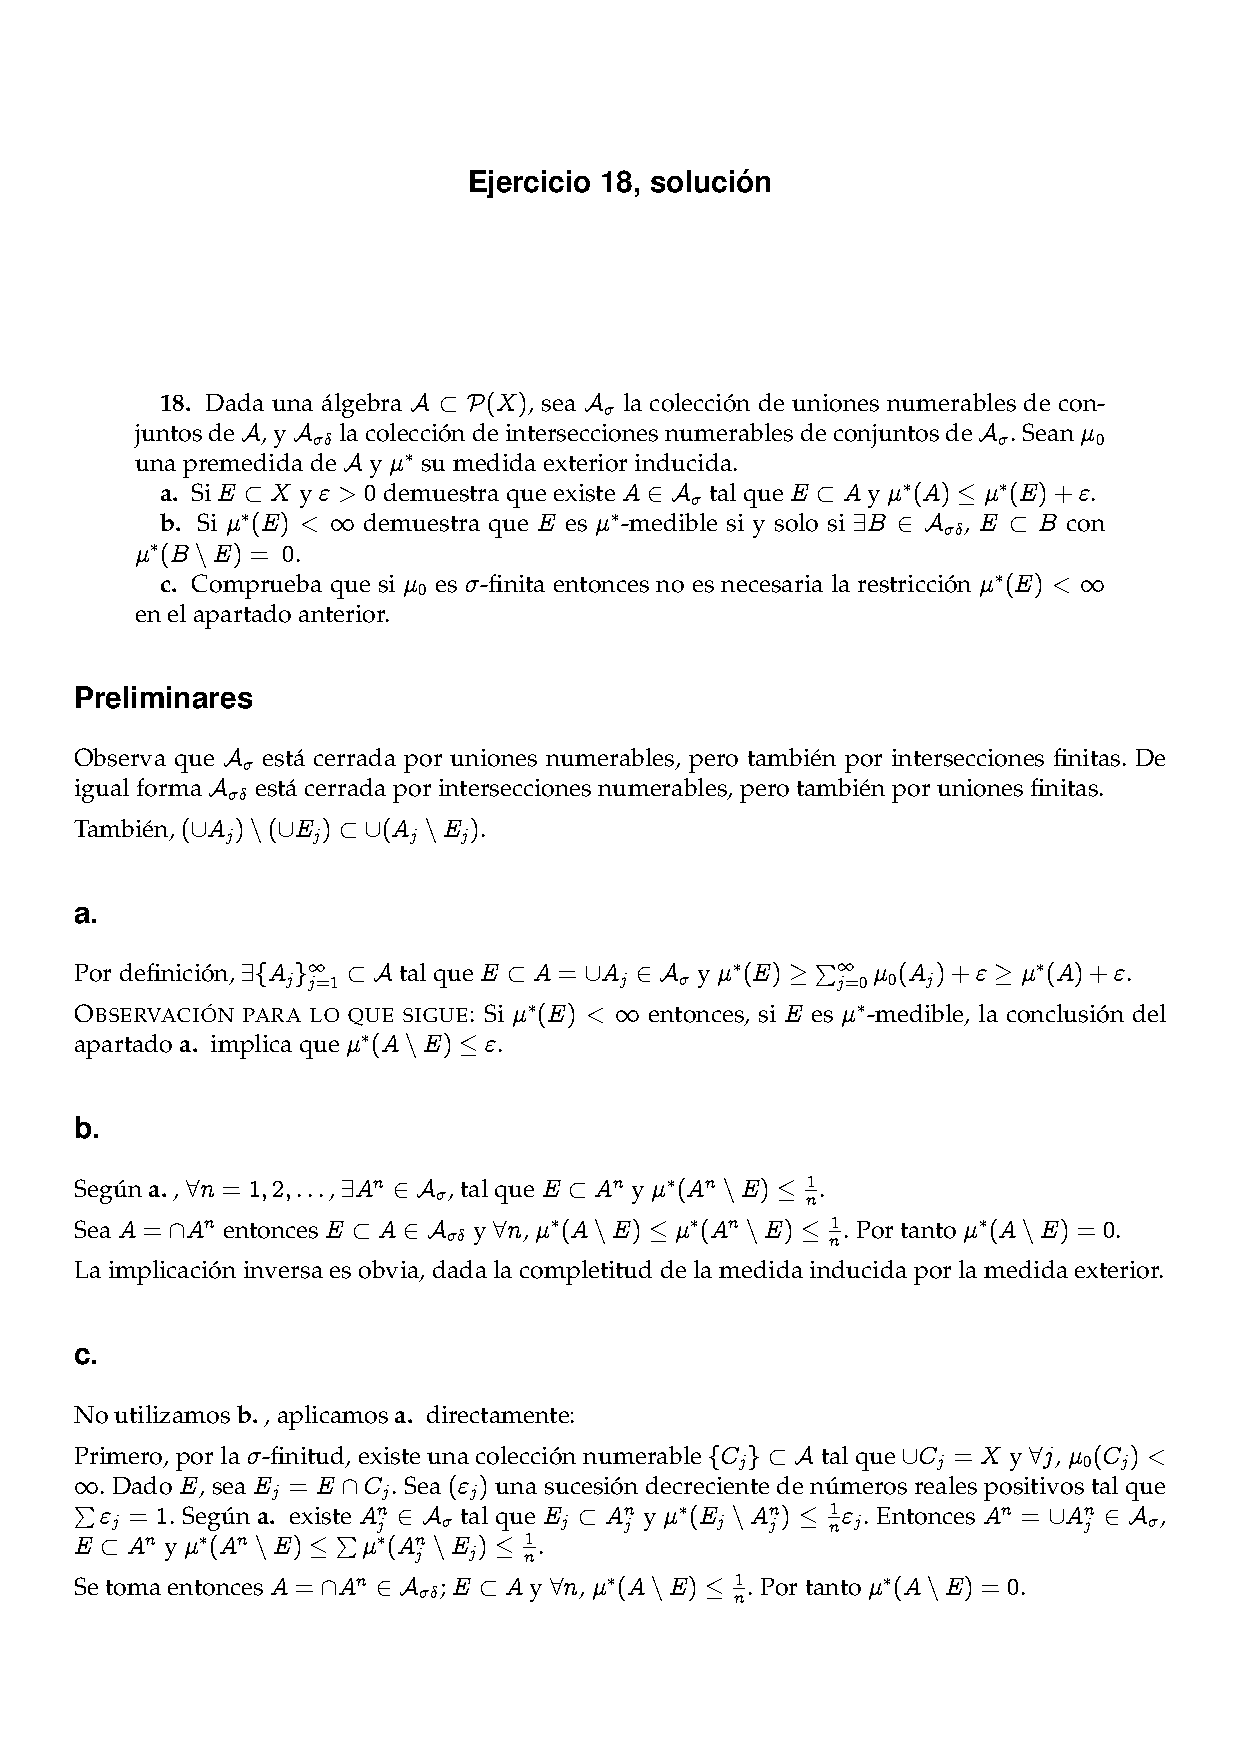
\includepdf[scale=0.9]{pdf/2014-03-18.pdf}
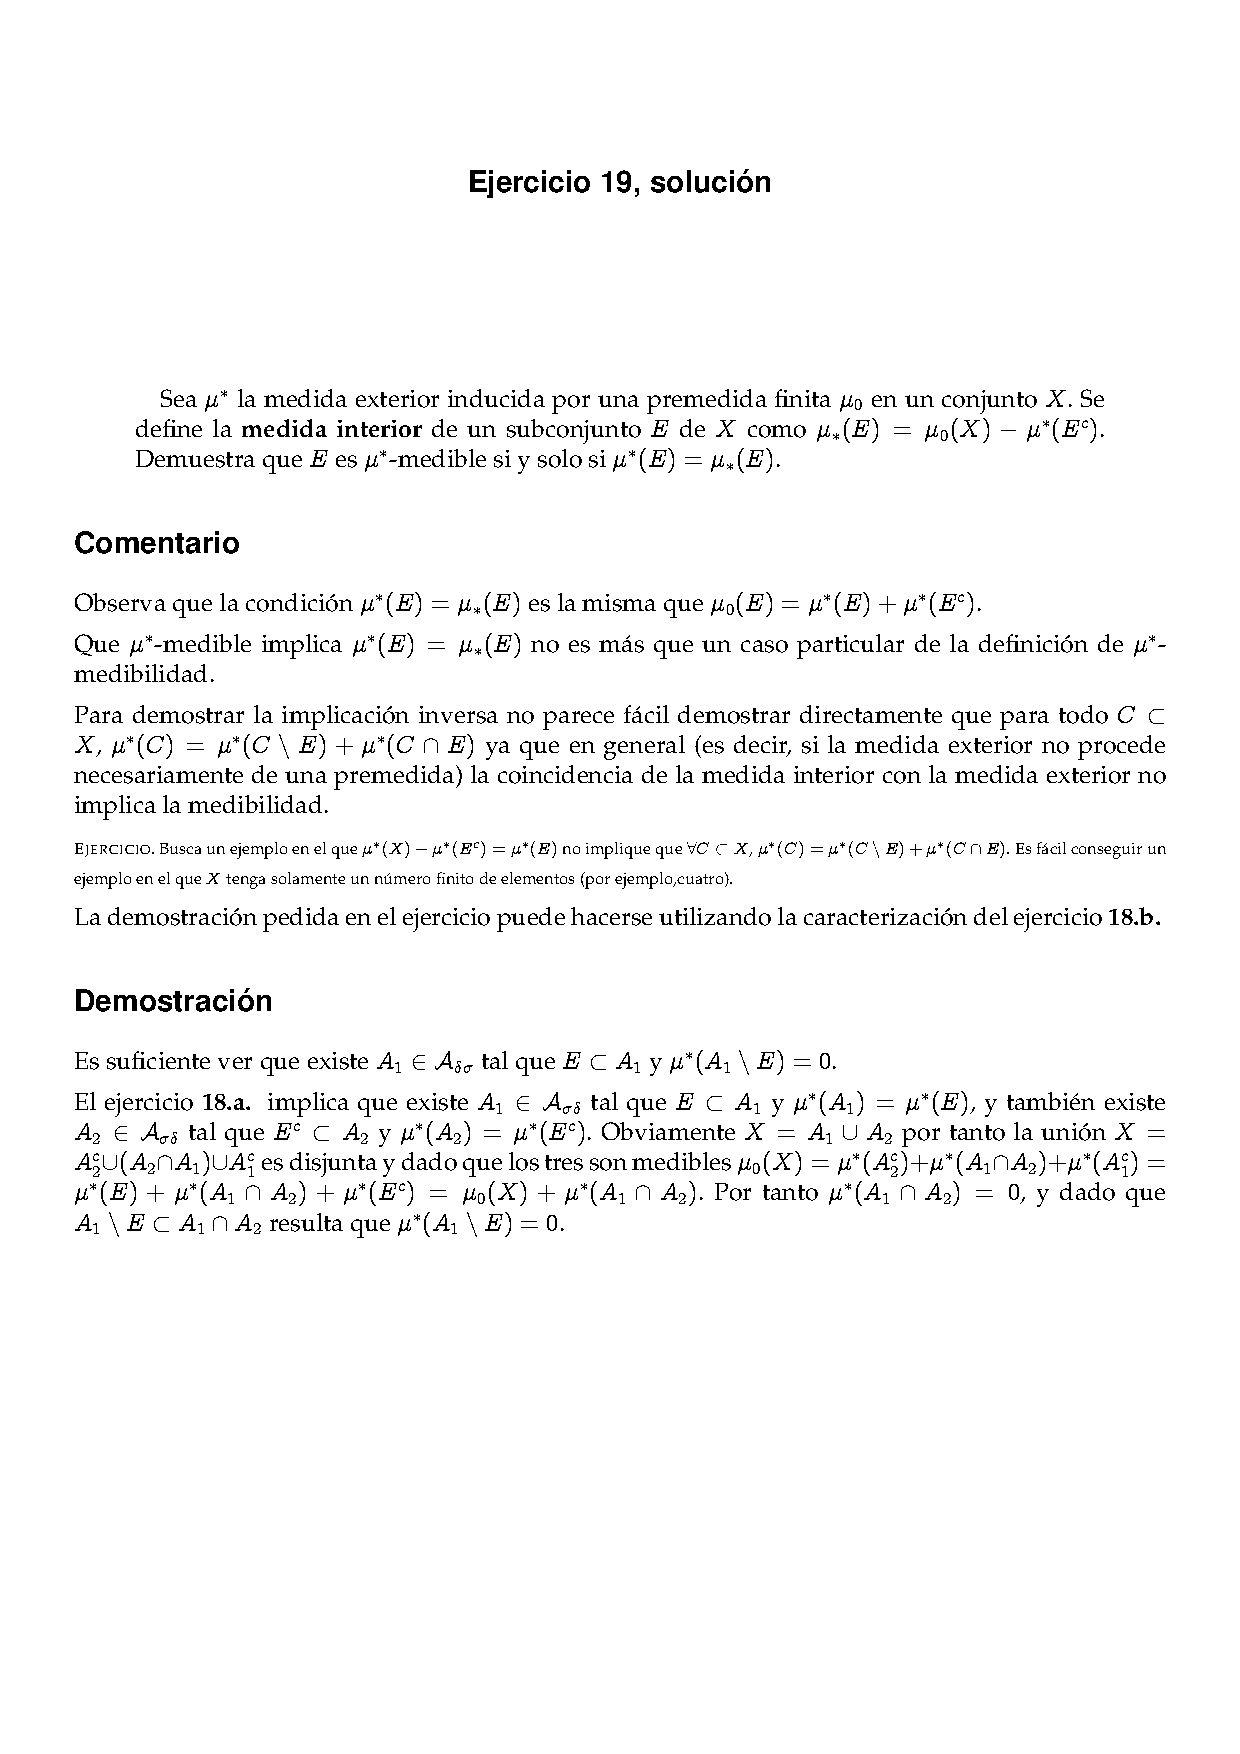
\includepdf[scale=0.9]{pdf/2014-03-19.pdf}
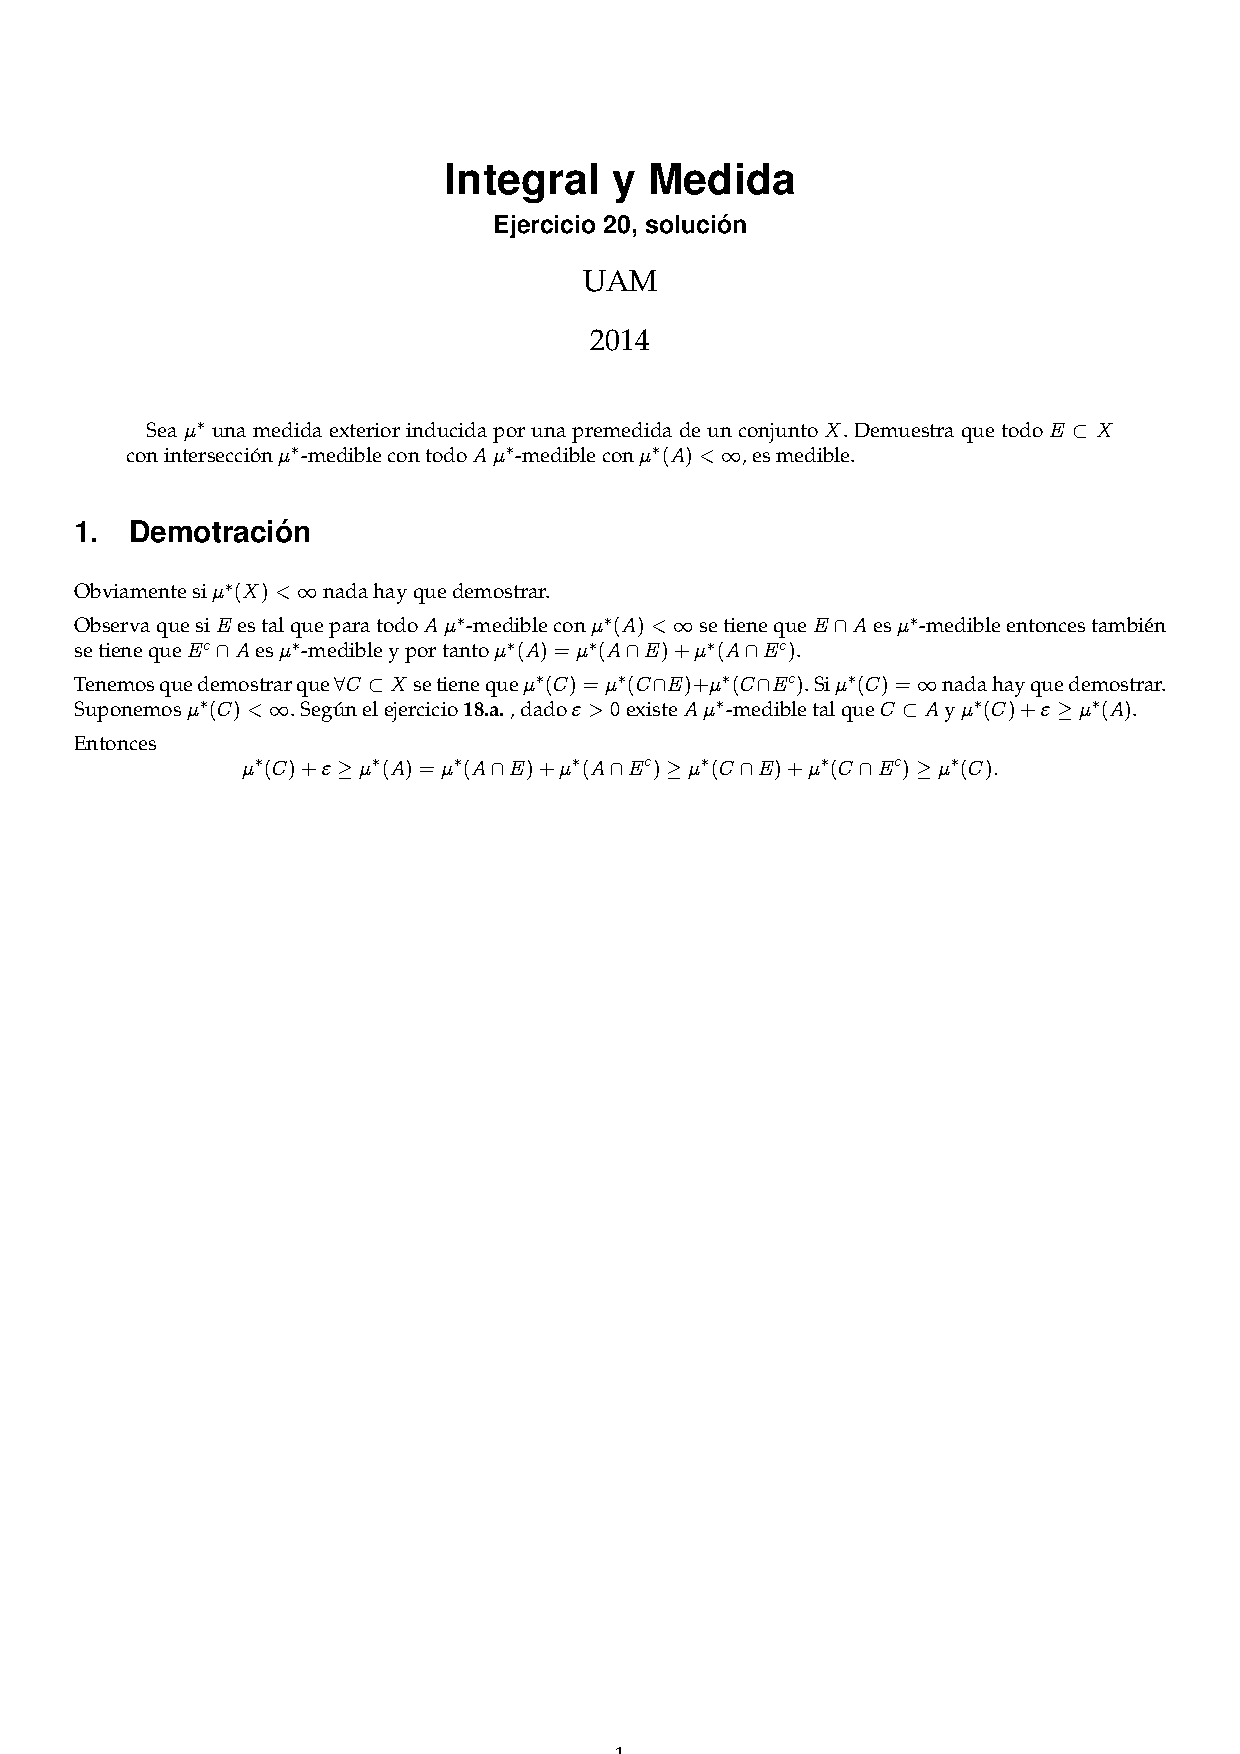
\includepdf[scale=0.9]{pdf/2014-03-20.pdf}

\subsection{Hoja 4}

\begin{problem}
Sea µ la medida de Lebesgue-Stieltjes asociada a la función:
\[F(x)=\left\{ \begin{array}{lcc}
             0 &   \text{si}  & x < 1 \\
             \\ x & \text{si} & 1 \leq x < 3 \\
             \\ 4 &  \text{si}  & 3 \leq x
             \end{array}
   \right.\]

Calcula las siguientes medidas:
\solution
\begin{itemize}
\item $µ(\{1\}) = F(1)-\displaystyle\lim_{x \to 1^-} F(x)$ = 1
\item $µ(\{2\}) = 0$
\item $µ((1, 3]) = F(3)-F(1) = 4 - 1 = 3$
\item $µ((1, 3)) = µ((1, 3]) - µ(\{3\}) = 3 - 1 = 2$
\item $µ([1, 3)) = µ((1, 3)) + µ(\{1\}) = 2 + 1 = 3$
\item $µ([1, 3])) = µ((1, 3]) + µ (\{1\}) = 3 + 1 = 4$
\end{itemize}
\end{problem}

\begin{problem}
Halla funciones de distribución $F$, $F_1$, $F_2$ de forma que, en cada caso, existan $a$ y $b$ tales que:
\begin{enumerate}
\item $µ((a,b)) < F(b)-F(a) < µ([a,b])$, donde $µ=µ_F$
\item $µ_1((a,b)) < µ_1((a,b]) < µ_1([a,b)) < µ_1([a,b])$ y

$µ_2((a,b)) < µ_2([a,b)) < µ_2((a,b]) < µ_2([a,b])$ donde $µ_i = µ_F, \ i=1,2$
\end{enumerate}
\solution
\begin{enumerate}
\item Vale con la función del ejercicio anterior
\item
\textbf{Con i = 1}
\[F_1(x)=\left\{ \begin{array}{lcc}
             0 &   si  & x < 1 \\
             \\ x & si & 1 \leq x < 3 \\
             \\ 3.5 &  si  & 3 \leq x
             \end{array}
   \right.\]

\textbf{Con i = 2}
\[F_2(x)=\left\{ \begin{array}{lcc}
             0 &   si  & x < 1 \\
             \\ x & si & 1 \leq x < 3 \\
             \\ 5 &  si  & 3 \leq x
             \end{array}
   \right.\]
\end{enumerate}

La construcción de estas funciones se ha realizado por la cuenta de la vieja. Si repetimos los cálculos del ejercicio anterior con estas funciones podemos ver que se cumplen las condiciones pedidas (Incluso puede que entendamos de qué va esto)
\end{problem}

\begin{problem}
Sea µ la medida de contar en $(\real, \algbP(\real))$. Para un conjunto finito A $\subset \real$ se define $µ_A(B) = µ(B \cap A)$ para todo $B \subset \real$

\ppart Sea $A=\{1,2,...,n,...\}$ ¿Es $µ_A$ una medida de Lebesgue-Stieltjes?. En caso afirmativo halla $F$ tal que $µ_A=µ_F$
\ppart Sea $A=\{\frac{1}{1},\frac{1}{2},...,\frac{1}{n},...\}$ ¿Es $µ_A$ una medida de Lebesgue-Stieltjes?. En caso afirmativo halla $F$ tal que $µ_A=µ_F$
\solution


\spart Esta medida simplemente cuenta el número de enteros positivos que hay en un conjunto $B$.

Por tanto, simplemente tenemos que buscar una función que realice esa misma función, por ejemplo:
\[F(x)=\left\{ \begin{array}{lcc}
             0 &   si  & 0 \leq x < 1 \\
             \\ n &  si  & n \leq x < n+1
             \end{array}
   \right.\]

Imitando las cuentas realizadas en el ejercicio 1 podemos que ver:
\begin{itemize}
\item $µ((1,3])) = F(3) - F(1) = 2$
\item $µ((1,3)) = µ((1,3])) - µ(\{3\}) = 2 - 1 = 1$
\end{itemize}
observamos que, efectivamente, obtenemos el número de enteros de cada intervalo.

\spart Esta medida cuenta el número de racionales de la forma $\frac{1}{n}$ que hay en un conjunto.

Esta medida no es de Lebesgue-Stieltjes. Una medida de Lebesgue-Stieltjes tiene que tener asociada una función $F$ como en el apartado anterior, es decir, tal que $μ((a,b]) = F(b) - F(a)$, y esta no puede tenerla.

Veamos por qué: tomemos el intervalo $B = (0,ε)$. Su medida según $μ_A$ es infinita, ya que para todo $n$ mayor que $\frac{1}{ε}$, $\frac{1}{n} ∈ A$, y entonces $B∩A$ es infinito. Luego tenemos que encontrar un $F$ tal que $F(ε) - F(0) = ∞$, y la única forma de que eso tenga sentido es que $F(ε) = ∞\; ∀ε$, lo cual es absurdo.

\end{problem}

\begin{problem}
Sea $F$ la función de distribución
\[F(x)=\left\{ \begin{array}{lcc}
             0 &   si  & x \in (-\infty, -1) \\
             \\ 1+x & si & x \in [-1, 0) \\
             \\ 2+x^2 & si & x \in [0, 2) \\
             \\ 9 &  si  & x \in [2, \infty)
             \end{array}
   \right.\]

Siendo $µ=µ_F$, hallar las siguientes medidas.
\solution
\begin{itemize}
\item $µ(\{2\}) = 3 $
\item $µ([-\frac{1}{2}, 3)) = 9 - \frac{1}{2}$
\item $µ((-1,0]\cup (1,2)) = 1 + µ((1,2]) - µ(\{2\}) = 1 + 9 -3 - 3 = 4$
\item $µ([0, \frac{1}{2}) \cup (1, 2]) = \frac{1}{4} + 6$
\item $µ(\{x \in \real \tq |x|+2x^2 > 1\})$=$µ((-\infty, -\frac{1}{2})) + µ((\frac{1}{2}, \infty)) = 0 + 9 - 2 - \frac{1}{4} = 7 - \frac{1}{4}$
\end{itemize}
\end{problem}

\begin{problem}
Sea $\appl{f}{\real}{\real}$ no negativa, integrable Riemann sobre cada intervalo finito y tal que $\int_{-\infty}^{\infty}f(x)=1$.

Prueba que $F(x)=\int_{-\infty}^x f(y) \dif y$ es una función de distribución de probabilidad y que, además, $F$ es continua ($f$ es la función de densidad de $F$).

Si $f(x)=\ind_{[0,1]}$ hallar $F$

\solution
Simplemente tenemos que ver que $F$ es no decreciente, continua por la derecha y que se cumple:
\[\lim_{n \to - \infty}F(x)=0 \ \ \lim_{n \to \infty}F(x)=1\]

Observando que $F$ es una integral y que integrar una función equivale a calcular el área encerrada bajo ella, vemos que a medida que avanzamos la $x$, cada vez estamos calculando un área mayor, luego los dos límites anteriores se cumplen.

Para ver que es continua por la derecha observamos que:
\[ \lim_{h \to 0^+}F(x+h) = \lim_{h \to 0^+} \int_{-\infty}^{x+h}f(y)\dif y = \int_{-\infty}^xf(y)\dif y = F(x)\]

Y es que por ser $F$ una integral, es obvio que es continua.

Suponemos ahora $f(x)=\ind_{[0,1]}$, para responder a la segunda pregunta del enunciado. Entonces
\[F(x)= \int_{-\infty}^{x} \ind_{[0,1]} = \left\{ \begin{array}{lcc}
             0 &   si  & x < 0 \\
             \\ x & si &  0 \leq x \leq 1 \\
             \\ 1 &  si  & 1 \leq x
             \end{array}
   \right.\]
\end{problem}

\begin{problem}
Halla el valor de $k$ para que $f= kx(1-x)\ind_{[0, 1)}$ sea la función de densidad de una medida de probabilidad. Calcula su función de distribución.

\solution
Para que sea función de densidad necesitamos que:
\[\int_{-\infty}^{\infty}f(x) dx = 1\]

Vamos a ver cuánto vale esa integral.
\begin{gather*}
\int_{-\infty}^{\infty}f(x) \dif x = \int_{-\infty}^{\infty}kx(1-x)\ind_{[0, 1)} \dif x  = \\
 = \int_{-\infty}^{0} kx(1-x)\cdot 0 \dif x + \int_{0}^{1}kx(1-x)\dif x + \int_{1}^{\infty}kx(1-x)\cdot 0 \dif x = \\
= k\left(\frac{1}{2}-\frac{1}{3}\right)
\end{gather*}


De donde obtenemos fácilmente que $k = \frac{1}{\frac{1}{2}-\frac{1}{3}} = 6$

La función de distribución sería:
\[\F(x)= \int_{-\infty}^{x} \ind_{[0,1]} = \left\{ \begin{array}{lcc}
             0 &   si  & x < 0 \\
             \\ \int_{0}^{x}kt(1-t)\dif t = (3x^2-2)x^3)& si &  0 \leq x \leq 1 \\
             \\ 1 &  si  & 1 \leq x
             \end{array}
   \right.\]
\end{problem}

\newpage
\begin{problem}
Dado $k$ > 0, sea $f(x)=αe^{-kx}\ind_{[0, \infty)}(x)$
\begin{enumerate}
\item Halla α para que $f$ sea una función de densidad de probabilidad
\item Sea $X$ una variable aleatoria con función de densidad f, si $k=\frac{1}{2}$, calcula la probabilidad de que $X \geq 3$
\item Si $k=\frac{1}{2}$ calcula la probabilidad de que $3 \leq X \leq 6$
\end{enumerate}
\solution
\begin{enumerate}
\item Repitiendo el proceso del ejercicio anterior, debemos hacer que $\int_{0}^{\infty}f(x)dx =1$.

En este caso obtenemos que α=k, es decir, nos encontramos ante una exponencial.

\item
\[\mathbb{P}(X \geq 3) = \int_{³}^{\infty}e^{-kx}dx=e^{\frac{3}{2}}\]

\item Puesto que la función de distribución es continua, la probabilidad de que $X=3$ ó $X=6$ es 0, de modo que podemos calcular la probabilidad pedida como:
\[\mathbb{P}(3 \leq X \leq 6) = \int_{3}^{6}e^{-kx}dx\]
\end{enumerate}
\end{problem}

\begin{problem}
Sea µ la medida de probabilidad definida por la función de distribución:

\[F(x)= \int_{-\infty}^{x} \ind_{[0,1]} = \left\{ \begin{array}{lcc}
             0 &   si  & x \in (- \infty, -1) \\
             \\ \frac{1}{3} & si &  x \in [-1, \sqrt{2}) \\
             \\ \frac{1}{2} + \frac{x-\sqrt{2}}{10} & si &  x \in [\sqrt{2}, 5) \\
             \\ 1 &  si  & x \in [5, \infty)
             \end{array}
   \right.\]

Calcular las siguientes medidas:
\solution

Antes de nada deberíamos comprobar que la función $F(x)$ dada es, efectivamente, una función de distribución. Para ello debemos comprobar que siempre es positiva y que se trata de una función creciente.

En este caso nos fiamos y se deja como ejercicio para el lector desconfiado (Edu) la comprobación de estas propiedades.
\newpage
\begin{enumerate}
\item \[µ((\real \setminus \rac)\cap[\sqrt{2}, 5]) = µ([\sqrt{2}, 5)) = µ((\sqrt{2}, 5]) + µ (\{\sqrt{2}\}) - µ (\{\sqrt{5}\}) =\]
\[ = F(5) - F(\sqrt{2}) +(\frac{1}{2}-\frac{1}{3}) -(1-(1-\frac{\sqrt{2}}{10}))=1-\frac{1}{2}+\frac{1}{6}-\frac{\sqrt{2}}{10}\]

\item \[µ((\real \setminus \rac)\cap [-2, \sqrt{2}]) = µ(\{\sqrt{2}\}) = \frac{1}{2}-\frac{1}{3} = \frac{1}{6}\]

\item \[µ(\rac \cap [1,6]) = µ(\{5\}) = \frac{\sqrt{2}}{10}\]
\end{enumerate}

Vamos ahora a por la parte complicada del ejercicio.

\[A_{3n-2} = \left(\frac{2n}{4n+3}, \frac{4n+5}{3n}\right)\]
\[A_{3n} = \left(\frac{4}{5n+2}, \frac{6n+1}{2n}\right)\]
\[A_{3n-1} = \left(-2, \frac{6n-1}{5n+2}\right)\]

Vemos que:
\begin{enumerate}
	\item $\lim A_{3n-2}= [\frac{1}{2}, \frac{4}{3}]$
	\item $\lim A_n{3n-1} = (-2, \frac{6}{5})$
	\item $\lim A_{3n} = (0^+, 3^+)$
\end{enumerate}

Recordemos que el límite superior de $A_n$ es el conjunto de puntos que están en infinitos conjuntos de la sucesión. Por tanto, todos los puntos contenidos en estos límites se contienen en el límite superior de la sucesión.
\[\limsup A_n = [\frac{1}{2}, \frac{4}{3}] \bigcup  (-2, \frac{6}{5}) \bigcup (0^+, 3^+)\]

Por otro lado, el límite inferior es el conjunto de puntos que se encuentran en todos los elementos de la sucesión a partir de uno dado. Así, el límite inferior será la intersección de los límites calculados anteriormente.
\[\liminf A_n = [\frac{1}{2}, \frac{4}{3}] \bigcap  (-2, \frac{6}{5}) \bigcap (0^+, 3^+)\]

\textcolor{blue}{Completado por mi. No fiarse al 100\%}
\[µ(\limsup A_n) = µ([\frac{1}{2}, \frac{4}{3}]) +  µ((-2, \frac{6}{5})) +µ((0^+, 3^+)) = \frac{1}{3}  + \frac{1}{3} + \frac{1}{3} = 1\]
\[µ(\liminf A_n) = µ([\frac{1}{2}, \frac{6}{5})) = 0\]

\end{problem}

\begin{problem}
Sea $\appl{F}{\real}{\real}$ una función de distribución
\begin{enumerate}
\item Prueba que el conjunto de puntos de discontinuidad de $F$ es numerable
\item Prueba que el conjunto de puntos de continuidad de $F$ es denso en $\real$
\end{enumerate}
\obs $F$ es monótona luego no tiene más discontinuidades que saltos
\solution

\begin{enumerate}
\item Vamos a probar que el número de puntos de discontinuidad en (n, n+1] es numerable.

Para ello tomamos la medida de este intervalo:
\[M = F(n+1)-F(n)\]

La pregunta que nos hacemos ahora es, ¿cuántos puntos $x \in (n, n+1]$ pueden tener $µ_F(\{x\}) \frac{M}{k}$?

La respuesta es sencilla (la supo hasta Elena en clase). $\forall k \in \nat$ No podemos tener más de k puntos con esta condición.

Por tanto no puede haber una cantidad no numerable de puntos de (n, n+1] con $µ_F(\{x\})>0$
%\item Si tuviésemos una cantidad no numerable de discontinuidades tendríamos un intervalo cerrado que contiene una cantidad no numerable de discontinuidades. Puesto que cada una de esas discontinuidades tenemos un salto, resulta que tendríamos un número no numerable de saltos en un intervalo cerrado.

%Así, tendríamos que la medida del intervalo cerrado sería la suma infinita y no numerable de valores positivos, lo que nos daría un resultado finito.

%Leyendo de un artículo de wikipedia:
%\begin{verbatim}
%La suma de los saltos no puede ser mayor que la diferencia de los
%valores de la función en los extremos del intervalo, de modo que
%el conjunto de discontinuidades con salto mayor que 1/n es finito
%y, por tanto, el conjunto de discontinuidades es a lo más numerable
%\end{verbatim}

\item \textcolor{blue}{Hecho por mi. No fiarse al 100\%}

Recordando lo dado en topología, sabemos que un conjunto es denso si la adherencia del conjunto coincide con el total.

Recordamos también que la adeherencia son aquellos puntos tales que todo abierto que lo contenta corta al conjunto dado.

Puesto que las únicas discontinuidades que puede presentar una función de distribución son discontinuidades de salto y es obvio que para cualquier punto en que la función sea continua todo entorno del punto contiene otros puntos de discontinuidad.
\end{enumerate}
\end{problem}

\begin{problem}
Variando si es necesario en cada caso el tamaño de los intervalos, construir un conjunto de tipo Cantor cuya medida de Lebesgue sea mayor que 1-ε
\solution
La construcción del conjunto de Cantor consiste en tomar el intervalo [0,1] y los siguientes conjuntos:
\begin{enumerate}
\item Construimos un intervalo $A_1$ de longitud $\frac{ε}{2}$ centrado en el intervalo [0,1].
\item Construimos $A_2 = \bigcup (a_i, b_i)$ tales que cada elemento de la unión tiene longitud igual a $\frac{1}{2}\frac{ε}{4}$.
\item etc
\end{enumerate}
Así, en el paso n-ésimo tenemos:
\[A_n = (a_1^n,b_1^n) \cup (a_2^n,b_2^n) \cup ... \cup (a_n^n,b_n^n)\]
donde cada intervalo de la unión tiene longitud $\frac{1}{2^{n-1}}\frac{ε}{2}$.

El conjunto de Cantor se obtiene restando del intervalo incial todos los intervalos $A_n$ que hemos ido construyendo. Es decir:
\[C = I -\bigcup A_n\]
\[m(C)=m(I)-\sum m(A_n) = 1 - ε\]
\end{problem}

\begin{problem}
Sea $µ_F$ la medida de Lebesgue-Stieltjes correspondiente a una función creciente y continua $\appl{F}{\real}{\real}$
\begin{enumerate}
\item Prueba que si A es numerable entonces $µ_F(A)$=0
\item Prueba que existen conjuntos A tales que $µ_F(A)> 0$ y A no contiene ningún intervalo abierto.
\item Si $µ(A)\geq 0$ y $µ(\real \setminus A) = 0$, ¿tiene que ser A denso en $\real$
\end{enumerate}
\obs Se recomienda construir una función $F(x)$ que sea constante en un intervalo
\solution

\begin{enumerate}
\item \textcolor{blue}{Hecho por mi. No fiarse al 100\%}

Si $A$ es numerable podemos escribirlo de la forma:
\[A = \bigcup_{i=1}^{\infty}\{a_i\} \tq a_i \neq a_j \forall i, j \ i \neq j\]
por tanto,
\[µ(A) = \sum_{i=1}^{\infty} µ(\{a_i\}) \]
pero, puesto que la función del enunciado es continua, la medida de un único punto siempre es 0 y por lo que
\[µ(A) = \sum_{i=1}^{\infty} µ(\{a_i\}) = \sum_{i=1}^{\infty}  0 = 0\]

\item Podemos tomar el conjunto $(a, b]$ que tendrá
\[µ((a,b]) = F(b)-F(a) \geq 0\]
ya que $F$ es creciente.

Ahora debemos cuida que no contenta abiertos. Para ello basta con tomar la intersección de este intervalo con los racionales.

Con ello eliminamos la posibilidad de que haya abiertos contenidos en el conjunto y mantenemos la medida del conjunto puesto que la medida de los racionales (que son los que estamos extrayendo) es 0.

\item No tiene por qué ser A denso. Pongamos un contraejemplo para probarlo.

Si tomo una función que crece entre el 0 y el 1 y luego se queda constante y tomo $A=(0,1)$ tenemos que se cumplen las condiciones del enunciado pero obviamente el intervalo $(0,1)$ en $\real$ no es denso.
\end{enumerate}
\end{problem}

\begin{problem}
Sea $F(x)=log(1 + |x|)\cdot \ind_{[0, \infty)}(x)$
\begin{enumerate}
\item Comprueba que $\appl{F}{\real}{\real}$ es creciente y continua por la derecha.
\item Calcula $µ_F(\{Cantor\})$
\end{enumerate}
\obs El conjunto de Cantor está contenido en $2^n$ intervalos de longitud $\frac{1}{3^n}$
\solution

\begin{enumerate}
\item \textcolor{blue}{Hecho por mi. No fiarse al 100\%}

Tenemos que ver que $a<b \implies F(a) < F(b)$ lo cual es obvio ya que el logaritmo es creciente y la función indicatriz simplemente vale 0 cuando $x4 < 0$ y 1 en el resto de casos.

Para ver que es contínua por la derecha necesitamos probar que:
\[\lim_{x \to a^+}F(x) = F(a) \ \forall a \in X\]
El único punto donde podemos dudar es en $a=0$ pero en ese caso está claro que:
\[\lim_{x \to 0^+}F(x) = \log(1) = 0 = F(0)\]

\item
\begin{defn}[Conjunto de Cantor]
Es el conjunto de todos los puntos del intervalo real [0,1] que admiten una expresión en base 3 que no utilice el dígito 1
\end{defn}

\[µ_F(\{Cantor\}) = 1 - \frac{1}{3}+2\frac{1}{9}+4\frac{1}{27}+... = \frac{1}{3} \sum_{n=1}^{\infty}\left(\frac{2}{3}\right)^{n-1} = \frac{1}{3} \frac{1}{1-\frac{2}{3}} = 1-1 = 0\]

\end{enumerate}
\end{problem}

\begin{problem}
Sea µ una medida de Borel en $\real$, finita sobre compactos, con $µ((0, 1])=1$
\begin{enumerate}
\item Prueba que si $\forall s \in \real, µ(s + E)=µ(E)$, entonces µ es la medida de Lebesgue.
\item Prueba que si $\forall s \in \real, µ(rE)=|r|µ(E)$, entonces µ es la medida de Lebesgue
\end{enumerate}
\solution
\begin{enumerate}
\item
Para ver que es la medida de Lebesgue necesitamos ver que
\[\forall a,b \ a<b \ µ((a,b]) = b-a\]
Por continuidad podemos restringirnos a trabajar con a,b racionales.

Por la invarianza por traslaciones es suficiente ver:
\[\forall b \in \rac \ µ((0,b])=b\]

Vamos a ello pues
\[µ((0, \frac{p}{q}]) = \sum_{i=1}^{\infty} µ((\frac{1-i}{q}, \frac{i}{q}]) = p\cdot µ((0, \frac{1}{q}])\]

Ahora sólo nos queda ver que $µ((0, \frac{1}{q}]) = \frac{1}{q}$, pero para ello basta con fijarnos en que:
\[µ((0, 1]) = \sum_{i=1}^{\infty} µ((\frac{i-1}{q}, \frac{i}{q}]) = q \cdot µ((0, \frac{1}{q}])\]

\item Se hace prácticamente igual que el apartado anterior. Se deja como ejercicio para casa.


\end{enumerate}
\end{problem}

\begin{problem}
Sea µ la medida de Lebesgue de $\real$ y $E \subset \real$ medible Lebesgue tal que 0 < µ(E) < $\infty$. Demuestra que para todo α, 0<α<1, existe un intervalo abierto I tal que µ($I \cap E$) > α m(I)
\solution
Sabemos que la medida de Lebesgue se puede aproximar bien por abiertos que contengan al conjunto $E$, es decir:
\[\forall ε > 0 \ \exists A \text{ abierto con } E \subset A \tq µ(E) > µ(A)-ε \]

Tomamos $A= \bigcup_{k=1}^{\infty} I_k$ con los $I_k$ disjuntos.

Suponemos ahora que $\exists α \in (0,1) \tq \forall I \text{ intervalo abierto } µ(E \cap I)\leq αµ(I)$
Entonces
\[µ(E) = \sum_{k=1}^{\infty}µ(E \cap I_k) \leq \sum_{k=1}^{\infty} α µ(I_k) = α µ(A)\]

Si la suposición fuese cierta tendríamos ahora
\[µ(A)-µ(E) \geq µ(A) - α µ(A) (1-α)µ(A) \geq (1-α)µ(E) > ε\]
y llegamos a contradicción.
\end{problem}


\newpage
\printindex
\end{document}
